%%% Define the actual document parameters:
% as of Dec 2022, formatting guide requires margins be "consistent on all sides"
% i.e., use oneside
\documentclass[oneside,11pt,letterpaper,openany]{report}


%%%  Include packages used throughout the dissertation:
\usepackage[export]{adjustbox}
\usepackage{afterpage}
\usepackage{algorithmic}
% \usepackage{algpseudocode}
\usepackage{amssymb}
\usepackage{amsmath,amssymb,amsfonts}
\usepackage{array}
\usepackage[base]{babel}
\usepackage{booktabs}
\usepackage{calc}
\usepackage{caption}
\usepackage{cite}
\usepackage[usenames,dvipsnames]{color}
\usepackage[usenames,dvipsnames]{colortbl}
\usepackage{comment}
\usepackage{csquotes}
\usepackage{csvsimple}
\usepackage{epsfig}
\usepackage{etoolbox}
\usepackage{fancyhdr}
% \usepackage{filecontents}
\usepackage{floatpag}
\floatpagestyle{plain}
\usepackage[T1]{fontenc} % adapted from https://tex.stackexchange.com/a/388208
\usepackage[hmarginratio=1:1,margin=1in]{geometry}
\usepackage{graphicx}
\usepackage{graphics}
\usepackage{grffile} % https://tex.stackexchange.com/a/110518
\usepackage{hyperref,cleveref}
\usepackage{ifthen}
\usepackage{import}
\usepackage{layout}
\usepackage{listings}
\usepackage{longtable}
\setlength{\LTleft}{0pt} % adapted from https://tex.stackexchange.com/a/48558
\usepackage{lscape}
\usepackage{makecell}
\usepackage[footnotes,definitionLists,hashEnumerators,smartEllipses,hybrid]{markdown}
\usepackage{makecmds}
\usepackage[framemethod=tikz]{mdframed}
\usepackage{morewrites}
\usepackage[resetlabels]{multibib}
% for compatibility with subrepos
% \citepinappendix not invoked in dissertation
\newcites{inappendix}{Supplementary References}
\usepackage{multirow}
\usepackage{moreverb}
\usepackage{natbib}
\usepackage{numprint}
\npthousandsep{\,}
\usepackage{pdflscape}
\usepackage[section]{placeins}
\usepackage{pythonhighlight}
\usepackage{rotating}
\usepackage{sectsty}
\usepackage{setspace}
\usepackage{siunitx}
\usepackage{stringstrings}
\usepackage{subcaption}
\usepackage{tabulary}
\usepackage{tabularx}
\usepackage{tabu}
\usepackage{titlesec}
\usepackage{textcomp}
% \usepackage[euler]{textgreek}
\usepackage[absolute]{textpos}
\setlength{\TPHorizModule}{8.5in}
\setlength{\TPVertModule}{11in}
\usepackage[flushleft]{threeparttable}
\usepackage{tocloft}
\usepackage{url}
\urlstyle{same}
\usepackage{vcell}
% \usepackage[table,xcdraw]{xcolor}
\usepackage{xfp}
\usepackage{xparse}
\usepackage{xstring}
% tikz must load after xcolor, https://tex.stackexchange.com/a/51490
\usepackage{tikz}
% \usepackage [latin1]{inputenc}

\usetikzlibrary{calc}

% pragma once, adapted from https://tex.stackexchange.com/a/195173
\makeatletter
\let\pragma@iinput=\@iinput
\def\@iinput#1{\xdef\@pragmafile{#1}\pragma@iinput{#1}}
\def\@pragmafile{default}
\def\pragmaonce{%
   \csname pragma@\@pragmafile\endcsname
   \global\expandafter\let \csname pragma@\@pragmafile\endcsname = \endinput
}
\makeatother


%%% Load all the setup code, which was originally in this file
\let\tiny\relax
\let\scriptsize\relax
\let\footnotesize\relax
\let\small\relax

% allow for large numbers of floats without
% https://tex.stackexchange.com/a/241006
\extrafloats{1024}

%%% Colors for tracking changes. %%%
%%% Use: \cut{<Text you want to cut.>} -> Makes the text red.
%%% Great for tracking changes that you send to advisor/committee.
\newcommand*\cut{\textcolor{red}}
\newcommand*\add{\textcolor{ForestGreen}}
\newcommand*\alter{\textcolor{blue}}

% ensure no headers have font size greater than 14
\sectionfont{\fontsize{14}{15}\selectfont}
\subsectionfont{\fontsize{12}{15}\selectfont}

% graduate school requires chapter headings be formatted like sections
% with no larger than 14pt font for chapter headings
% adapted from https://tex.stackexchange.com/a/10332
\titleformat{\chapter}[block]
  {\normalfont\fontsize{14}{15}\selectfont\bfseries\centering}
  {\chaptername{} \thechapter\\}
  {0em}
  {}

% part headings also can't be bigger than 14pt
\partfont{\fontsize{14}{15}\selectfont}

% adapted from https://tex.stackexchange.com/a/53340
\titlespacing{\section}{0pt}{6pt}{0pt}
\titlespacing{\subsection}{0pt}{6pt}{0pt}
\titlespacing{\subsubsection}{0pt}{6pt}{0pt}
\titlespacing{\chapter}{0pt}{-7pt}{0pt}



% documentation for the spacing, title format, section format: https://ctex.org/documents/packages/layout/titlesec.pdf

%%%%%%%%%%%%%%%%%%%%%%%%%%%%%%%%%%%%%%%%%%%%%%%%%%%%%%%%%%%%%%%%%%%%%%%%%%%%%%

%%% Use the following to format your titles for the Table of Contents, List of Figures, List of Tables.
%\renewcommand{\cfttoctitlefont}{\normalfont\Large\bfseries\MakeUppercase}
% ---- 2021-05-06 - pre-msu-revision ----
% \setlength{\cftbeforetoctitleskip}{-0.2in}
% \setlength{\cftaftertoctitleskip}{0.1875in}
% ------
\setlength{\cftaftertoctitleskip}{0in}
\setlength{\cftbeforetoctitleskip}{-0.5em}
\renewcommand{\cfttoctitlefont}{\hfill\bfseries}
\renewcommand{\cftaftertoctitle}{\hfill}
\renewcommand{\contentsname}{\centerline{TABLE OF CONTENTS}}

% adapted from http://tug.ctan.org/tex-archive/macros/latex/contrib/tocloft/tocloft.dtx
% adapted from https://tex.stackexchange.com/a/498313
\makeatletter
  \renewcommand{\@tocrmarg}{2.55em plus 1fil}
\makeatother

% ensure that parts are labeled as such in toc
% ... have to hack Part into font because
% \renewcommand{\cftpartpresnum}{Part }
% has no effect
% see https://tex.stackexchange.com/questions/419428/
\renewcommand\cftpartfont{\bfseries Part~}
\renewcommand\cftchapfont{}
\renewcommand\cftsecfont{}

\renewcommand\cftpartpagefont{\bfseries}
\renewcommand\cftchappagefont{}
\renewcommand\cftsecpagefont{}

\setlength{\cftbeforepartskip}{1pc}
\setlength{\cftbeforechapskip}{1pc}
\setlength{\cftbeforesecskip}{0pc}

% MSU now only requires (and prefers) chapters to be listed
\setcounter{tocdepth}{0}
% Add dot leaders to the chapter entries in the TOC
\renewcommand{\cftpartleader}{\bfseries\cftdotfill{\cftdotsep}}
\renewcommand{\cftchapleader}{\cftdotfill{\cftdotsep}}

% \setlength{\cftbeforeloftitleskip}{-0.17in}
% \setlength{\cftafterloftitleskip}{0.1875in}
% \renewcommand{\cftloftitlefont}{\hfill\Large\bfseries}
% \renewcommand{\cftafterloftitle}{\hfill}
% \renewcommand{\listfigurename}{\large\centering{LIST OF FIGURES}}

% \setlength{\cftbeforelottitleskip}{-0.33in}
% \setlength{\cftafterlottitleskip}{0.3875in}
% \renewcommand{\cftlottitlefont}{\hfill\Large\bfseries}
% \renewcommand{\cftafterlottitle}{\hfill}
% \renewcommand{\listtablename}{\large\centering{LIST OF TABLES}}

%%% Bibliography setup for TOC and The Final Page %%%%
\renewcommand{\bibname}{\vspace*{-0.95in} \large\centering{BIBLIOGRAPHY}}

%%% Put colon after figure number in the list of figures %%%
% \renewcommand{\cftfigpresnum}{Figure\ }
% \renewcommand{\cftfigaftersnum}{:\ }

%%% Put Table before and colon after table number in the list of tables %%%
% \renewcommand{\cfttabpresnum}{Table\ }
% \renewcommand{\cfttabaftersnum}{:\ }

% Put spacing after the Table #: and Figure #: in the LOF and LOT
\newlength{\mylenf}
\settowidth{\mylenf}{\cftfigpresnum}
\setlength{\cftfignumwidth}{\dimexpr\mylenf+0.35in}
\setlength{\cfttabnumwidth}{\dimexpr\mylenf+0.35in}

% Use this in conjunction with making the LOT singlespace so that long table entries are
% single space within entries and double space between entries
\renewcommand\cfttabafterpnum{\vskip\baselineskip}

%%% Put Chapter before number in the TOC %%%
\renewcommand\chaptername{Chapter}
\renewcommand\cftchappresnum{\chaptername\space}
\setlength{\cftchapnumwidth}{\widthof{\textbf{Chapter~999~}}}


%%%%%%%%%%%%%%%%%%%%%%%%%%%%%%%%%%%%%%%%%%%%%%%%%%%%%%%%%%%%%%%%%%%%%%%%%%%%%%

\fancypagestyle{mylandscape}{%
  \fancyhf{}% Clear header/footer
  \fancyfoot{% Footer
  % adapted from https://tex.stackexchange.com/a/9086
  \tikz[remember picture,overlay]
        \node[outer sep=0.5in,above,rotate=90] at (current page.east) {\thepage};}  \renewcommand{\headrulewidth}{0pt}% No header rule
  \renewcommand{\footrulewidth}{0pt}% No footer rule
}

% adapted from https://tex.stackexchange.com/a/472608
\usepackage{eso-pic,zref-user}
\newcounter{cntsideways}
\makeatletter
\AddToShipoutPictureBG{%
  \PLS@RemoveRotate
}
\AddToShipoutPictureBG{%
 \ifnum\zref@extractdefault{rotate\number\value{page}}{page}{0}=0
  \PLS@RemoveRotate
 \else
  \PLS@AddRotate{90}%
 \fi}

\newcommand\rotatesidewayslabel{\stepcounter{cntsideways}%
 \zlabel{tmp\thecntsideways}\zlabel{rotate\zref@extractdefault{tmp\thecntsideways}{page}{0}}}

\let\originalsidewaysfigure\sidewaysfigure
\let\endoriginalsidewaysfigure\endsidewaysfigure
\renewenvironment{sidewaysfigure}{%
  \begin{originalsidewaysfigure}%
  \thisfloatpagestyle{mylandscape}%
  \rotatesidewayslabel%
}{%
  \end{originalsidewaysfigure}%
}
\renewenvironment{sidewaysfigure*}{%
  \begin{originalsidewaysfigure}%
  \thisfloatpagestyle{mylandscape}%
  \rotatesidewayslabel%
}{%
  \end{originalsidewaysfigure}%
}

\let\originalsidewaystable\sidewaystable
\let\endoriginalsidewaystable\endsidewaystable
\renewenvironment{sidewaystable}{%
  \begin{originalsidewaystable}%
  \thisfloatpagestyle{mylandscape}%
  \rotatesidewayslabel%
}{%
  \end{originalsidewaystable}%
}
\renewenvironment{sidewaystable*}{%
  \begin{originalsidewaystable}%
  \thisfloatpagestyle{mylandscape}%
  \rotatesidewayslabel%
}{%
  \end{originalsidewaystable}%
}

\let\originallandscape\landscape
\let\endoriginallandscape\endlandscape
\renewenvironment{landscape}{%
  \begin{originallandscape}%
  \thispagestyle{mylandscape}%
  \rotatesidewayslabel%
}{%
  \end{originallandscape}%
}

\makeatother

%%% Renew command for full page figures:
\renewcommand{\topfraction}{1.0}

% Blank page (if needed)
\newcommand\blankpage{%
    \null
    \thispagestyle{empty}%
    \addtocounter{page}{-1}%
    \newpage}

%%%  Set the margins as required by the MSU graduate school.
%%%  Specifically, set the margins 1 inch top bottom and right,
%%%  1.5 inch on left.  Now, Latex has margin origins at 1 in on the top
%%%  and left so for 1.5 in the margin is set at 1.5 - 1 = .5 inch
%\setlength{\oddsidemargin}{.5in}   % This is the left margin for both
%\setlength{\evensidemargin}{1.5in} % even and odd pages (in case you use the book format)
\setlength{\topmargin}{0in} % Top margin (remember latex starts from 1 in)

% Pagewidth(8.5in) - textwidth(6in) - leftmargins(1.5in) = 1 inch for right margin
\setlength{\textwidth}{6.5in}

% Page height (11in) - Topmargin (1in) - Textheight (1in) = 1 in for
%                                                      bottom margin
\setlength{\textheight}{9in} %
\setlength{\footskip}{.5in}
%%% Headings are not required, thus suppress:
\setlength{\headheight}{0in}
\setlength{\headsep}{0in}

\newsavebox{\savefig}


%%%%%%%%%%%%%%%%%%%%%%%%%%%%%%%%%%%%%%%%%%%%%%%%%%%%%%%%%%%%%%%%%%%%%%%%%%%%%%

% ensure all code listings have continuation labels
% adapted from https://tex.stackexchange.com/a/117839
\surroundwithmdframed[
  hidealllines=true,
  middleextra={
    \node[anchor=west] at (O|-P)
    {\lstlistingname{} \thelstlisting{}  (cont'd)};
  },
  secondextra={
    \node[anchor=west] at (O|-P)
    {\lstlistingname{} \thelstlisting{}  (cont'd)};
  },
  splittopskip=\baselineskip
]{lstlisting}

% % need to wrap lstimportlisting in dummy lstinputlistinghandle env
% in order for mdframed to attach
% BUT this approach appears to be to intensive on compiler memory use
% so, instead, wrap everything in mdframed directly
\newenvironment{lstinputlistinghandle}{}{}
\surroundwithmdframed[
  hidealllines=true,
  middleextra={
    \node[anchor=center] at ($(P)!0.5!(O|-P)$)
    {\lstlistingname{} \thelstlisting{}  (cont'd)};
  },
  secondextra={
    \node[anchor=center] at ($(P)!0.5!(O|-P)$)
    {\lstlistingname{} \thelstlisting{}  (cont'd)};
  },
  splittopskip=\baselineskip
]{lstinputlistinghandle}

\topskip=0pt

%%%  Include any definitions you wish to use throughout the dissertation
%%%  If you want to add helper functions, I recommend you do it here -- @AJF
%\newcommand{\thesisTitle}{Selection Pressures in the Evolutionary Transition from Reactive Phenotypic Plasticity to Early Learning}

%\newcommand{\thesisTitle}{Separating Historical Flukes from Evolutionary Inevitabilities: \\ An Empirical Analysis of Historical Contingencies}
\newcommand{\thesisTitle}{An Empirical Analysis of Historical Contingency in Evolution}

%\newcommand{\thesisTitle}{Evolutionary Fluke or Historical Inevitability? \\ Replaying the Origins of Early Cognitive Behaviors}
%\newcommand{\thesisTitle}{The Role of History in the Evolution of Early Cognitive Behaviors}

\newcommand{\authorName}{Austin James Ferguson}
\newcommand{\graduationYear}{2024}

\newcommand{\code}{\texttt}

\newcommand*{\theadalt}[1]{\multicolumn{1}{c}{\bfseries #1}}

% Add an easy-to-use tilda for approximations
\newcommand{\localapprox}{\raisebox{0.5ex}{\texttildelow}}

%%%%%%%%%%%%%%%%%%%%%%%%%%%%%%%%%%%%%%%%%%%%%%%%%%%%%%%%%%%%%%%%%%%%%%%%%%%%%%

%%%  Begin the actual dissertation:
\begin{document}
\raggedbottom
\sloppy
\pagenumbering{roman}
\pagestyle{empty}
\setlength{\parindent}{2 em}

%\layout

%%%%%%%%%%%%%%%%%%%%%%%%%%%%%%%%%%%%%%%%%%%%%%%%%%%%%%%%%
% == Title page ==
% This should be self contained unless you need to edit the degree
% Name and title are defined in x0_supporting_files/definitions.tex
% adapted from https://tex.stackexchange.com/a/601029
\begin{center}
  % title 2 inches from top of page
  \begin{textblock}{
     \fpeval{(8.5 - 2.0) / 8.5} % width
    }(
      \fpeval{1.0 / 8.5}, % xpos
      \fpeval{2.0 / 11.0} % ypos
    )
    \centering
    \MakeUppercase{\thesisTitle}
   \end{textblock}

   % By 3.5 inches from top of page
   \begin{textblock}{
      \fpeval{(8.5 - 2.0) / 8.5} % width
     }(
       \fpeval{1.0 / 8.5}, % xpos
       \fpeval{3.5 / 11.0} % ypos
     )
     \centering
     By
    \end{textblock}

    % author name 4 inches from top of page
    \begin{textblock}{
       \fpeval{(8.5 - 2.0) / 8.5} % width
      }(
        \fpeval{1.0 / 8.5}, % xpos
        \fpeval{4.0 / 11.0} % ypos
      )
      \centering
      \authorName
     \end{textblock}

    % document name 7 inches from top of page
    \begin{textblock}{
      \fpeval{(8.5 - 2.0) / 8.5} % width
     }(
       \fpeval{1.0 / 8.5}, % xpos
       \fpeval{7.0 / 11.0} % ypos
     )
     \centering
      A DISSERTATION % Check regulations for Masters
    \end{textblock}

    % submitted to 7.5 inches from top of page
    \begin{textblock}{
      \fpeval{(8.5 - 2.0) / 8.5} % width
     }(
       \fpeval{1.0 / 8.5}, % xpos
       \fpeval{7.5 / 11.0} % ypos
     )
     \centering
     Submitted to\\
     Michigan State University\\
     in partial fulfillment of the requirements\\
     for the degree of\\
    \end{textblock}

    % degree(s) 8.5 inches from top of page
    \begin{textblock}{
      \fpeval{(8.5 - 2.0) / 8.5} % width
     }(
       \fpeval{1.0 / 8.5}, % xpos
       \fpeval{8.5 / 11.0} % ypos
     )
     \centering
     Computer Science - Doctor of Philosophy\\
     Ecology, Evolution, and Behavior - Dual Major
    \end{textblock}

    % year 9 inches from top of page
    \begin{textblock}{
      \fpeval{(8.5 - 2.0) / 8.5} % width
     }(
       \fpeval{1.0 / 8.5}, % xpos
       \fpeval{9 / 11.0} % ypos
     )
     \centering
     \graduationYear
    \end{textblock}

\end{center}
\null\newpage

%%%%%%%%%%%%%%%%%%%%%%%%%%%%%%%%%%%%%%%%%%%%%%%%%%%%%%%%%
% == Abstract ==
% Loads from text from 00_prelim/abstract.tex
\begin{doublespace}
\centerline{\textbf{ABSTRACT}}

While evolution has created a stunning diversity of complex traits in nature, isolating the details for \textit{how} a particular trait evolved remains challenging.
Specifically, what were the critical events in evolutionary history that made that trait more or less likely to arise? %, or are most traits just flukes? 
We must consider historical contingency, where even small changes, such as an apparently neutral mutation, can have substantial influence on long-term evolutionary outcomes. 
Evolutionary biologists have long been interested in the role that historical contingency plays in evolution, but testing hypotheses of its effects has traditionally been difficult and time consuming, if it is even possible at all. 

Here I leverage the speed and power of digital evolution to experimentally test the role of historical contingency in evolution. 
I start by observing how the evolution of phenotypic plasticity stabilizes future evolutionary dynamics. 
Next, I employ analytic replay experiments to empirically test which mutations in a population's history increased the likelihood that associative learning evolves, first as case studies and then using more statistically powerful experimental approaches. 
I demonstrate that single mutations can drastically increase the odds of learning appearing, shifting it from a rare possibility to a near inevitability, and I find that these ``potentiating'' mutations exist in all studied lineages. 
%Finally, I demonstrate that potentiating mutations identified via replay experiments can highlight the importance of population disequilibrium in the adaptive momentum effect. 
Finally, I use potentiating mutations to develop an intuitive view into how adaptive momentum increases evolutionary exploration in populations experiencing disequilibrium. 

We are only beginning to scratch the surface of how historical contingency influences evolution, but digital evolution systems can expedite this process by testing these hypotheses and further refining these techniques for use in natural organisms. 
This work, and those like it, are pivotal in understanding how populations previously evolved, how their accumulated history currently affects them, and how they might evolve far into the future.
%Continuing to increase our understanding of historical contingency will not only help us understand how life evolved to its current state, but it will also help us predict how populations will continue to evolve. 
%A better understanding of history's role in evolution will help us understand how the organisms around us came to be, and also where they might be going in the future. 


% We can look at any organism around us, including ourselves, and ask how any particular trait of that organism came to be. 
% Indeed, this question can be asked at multiple levels. 
% Perhaps we are interested in the biochemical processes that give rise to neuron activation, or the prior evolutionary stepping stones that have led to echolocation in certain mammals. 
% I focus on one particular question: what were the critical events in the evolution of that trait? 
% We can point to possible candidates, 

% How do traits evolve? 

%%%%%%%%%%%% COMPS ABSTRACT BELOW VVVVVVVV


% % Set the stage that evolution is complicated but it becomes a tiny bit easier if we break it into component parts that we can quantify
% While evolution has created a stunning diversity of complex traits in nature, understanding \textit{how} a particular trait evolved remains a major challenge in evolutionary biology.
% Many dynamics can be at play during evolution, but are often summarized into three factors: adaptation (selective pressures), chance (stochastic events), and history (the genetic starting point for continued evolution).
% %Many dynamics can be at play during evolution, but researchers often boil these down into three key factors: adaptation, chance, and history. 
% %To aid in this endeavour, many researchers adopt the view that evolution is a composite of three factors: adaptation, chance, and history.
% The interplay among these factors can be complex and difficult to disentangle.
% %None of these factors operate in a vacuum; it is the interplay between them that creates the various evolutionary dynamics. 
% By conducting replay experiments on actively evolving populations, however, we can measure the role that each factor played in the evolution of a particular trait.
% Furthermore, these techniques allow us to study genotypes along the history of a linage in order to identify changes not only in phenotypic function, but in evolutionary potential.
% %Further, these studies can not only identify the role that each factor played, they can also identify \textit{when} key aspects of this evolution occurred. 

% % What are we doing, broadly?
% Here I propose to leverage and expand upon these experimental techniques in digital systems.
% I plan to investigate the role that history plays in the evolution of early cognitive behaviors such as associative learning and memory usage in navigation.
% Are there common building blocks whose evolution facilitates more complex behaviors?
% Does the likelihood of a trait evolving increase gradually or in bursts?
% What other elements should we consider that might influence the evolution of a trait?
% To get at these questions, I experimentally measure ``trait potentiation'' as the probability of a trait arising for a given starting population and evolutionary conditions.
% %I focus on how potentiation -- the likelihood a target trait evolves from a given genotype -- changes over the course evolved lineages.

% My use of digital systems allows me to conduct analytic replay experiments on a massive scale.
% Specifically, I can target individual points in evolutionary history and conduct replay experiments to measure their potentiation.
% By comparing potentiation before an after a given mutation, I am able to pinpoint specific mutations that affect potentiation.
% Points that increase potentiation inherently shift the evolution of a trait from requiring chance events to being able to rely on adaptive pressures.
% I will study lineages that ultimately lead to a trait of interest to determine if potentiation increases gradually or if the trait's appearance flips suddenly from fluke to inevitability.

% %switch the evolution of a focal trait from a fluke to an inevitability -- from chance to adaptation.  
% I have two main aims in this dissertation proposal: 
% 1) I want to understand the evolution of potentiation, and more broadly, how history interacts with adaptation and chance to produce complex traits and behaviors, and 
% 2) I want to explore how cognitive behaviors evolve, and more specifically, why these behaviors so rarely arise in digital evolution systems. 
% While these techniques have been refined over the last few decades, here I propose to conduct them on scales only feasible in digital systems.
% As described below, I will fully explore whole lineages, and even full fitness landscapes, while disentangling the effects of different traits, environments, and representations.
% My goal is to develop a more holistic understanding of how potentiation changes during evolution.


% % I will fully explore many successful (and some unsuccessful) lineages, isolating the effects of each mutation and, in case studies, disentangling their interactions with the background genomes.
% % Furthermore, I will conduct potentiation measures for each possible starting point in simple digital systems, to fully understand the potentiation landscape and how evolutionary dynamics interact with it.
% % to allow for the first cross-environment and cross-representation comparisons of how potentiation changes along lineages. 


% % What are we doing, per chapter?
% I start this proposal (Chapter \ref{chap:intro}) with a review of the relevant background in adaptation, chance, and history, as well as my own perspective on how I view these topics.  
% I also provide an overview of prior work on the evolution of cognitive behaviors in digital systems. 
% Next (in Chapter \ref{chap:learning_case_studies}) I demonstrate that single mutations can drastically increase the potentiation of associative learning, and follow that up with a proposal (Chapter \ref{chap:learning_distributions}) to expand the scale of this work to allow for deeper analyses and more powerful statistical comparisons. 
% In Chapter \ref{chap:adaptive_momentum}, I take a step back and examine potentiation in a simplified bitstring model, which I propose as a mechanism to better understand the basics of potentiation and how it relates to epistatic interactions. 
% Thinking about the role of history in evolution more broadly, in Chapter \ref{chap:consequences_of_plasticity} I discuss published investigations into how the evolution of phenotypic plasticity, a common stepping stone for cognitive behaviors, shapes future evolutionary dynamics.
% In order to assess the robustness of earlier results, in Chapter \ref{chap:adaptive_momentum} I propose to compare the associative learning potentiation work to new studies that I will conduct using my phenotypic plasticity environment as well as a new navigational behavior environment.
% Finally, in Chapter \ref{chap:conclusion}, I provide a timeline for this work and identify some additional assessments that should be performed in the future (or, perhaps, as alternatives to the chapters above).  For example, the underlying representations of the digital organisms could be varied to investigate the generalizability of patterns across organism types. 

% Overall, I believe that these studies will help us gain a deep understanding about the evolution of potentiation, with strong implications for the evolution of evolvability and ideally the prediction of evolutionary outcomes.

\end{doublespace}
\newpage

%%%%%%%%%%%%%%%%%%%%%%%%%%%%%%%%%%%%%%%%%%%%%%%%%%%%%%%%%
% == Copyright page ==
% Should be self contained in 00_prelim/02_copyright_page 
\vspace*{\fill}
{\raggedright
Copyright by\\
\MakeUppercase{\authorName}\\
\graduationYear
}
\vspace*{\fill}
\newpage

%%% Set the page numbering scheme:
% as of Dec 2022, roman page numbering must begin on the dedication page
\pagestyle{plain}

%%%%%%%%%%%%%%%%%%%%%%%%%%%%%%%%%%%%%%%%%%%%%%%%%%%%%%%%%
% == Dedication ==
% Edit via 00_prelim/03_dedication.tex
\vspace*{\fill}
\begin{hyphenrules}{nohyphenation}
\begin{center}
In memory of my grandmother, Mammaw Debbie. 

Oh, how I wish you were here to celebrate. 
\end{center}
\end{hyphenrules}
\vspace*{\fill}
\newpage

%%%%%%%%%%%%%%%%%%%%%%%%%%%%%%%%%%%%%%%%%%%%%%%%%%%%%%%%%
% == Ackowledgments ==
% Edit via 00_prelim/04_acknowledgemnts.tex
\begin{doublespace}
\centerline{
\textbf{ACKNOWLEDGEMENTS}
}
When writing a dissertation about historical contingency, it is impossible to avoid thinking about the events in my own life, both big and small, that have brought me to this point. 
Among all of the decisions, failures, and chance events that potentiated this path, the most important factors are the plethora of amazing people whose paths have crossed my own.
Here I wish to thank them.
Fully encapsulating my gratitude within this text is impossible, but I will try my best. 

To those who seemingly never tire: Barbara Bloemers, Vinny Mattison, Dr. Elise Zipkin, Dr. Sandeep Kulkarni, and Dr. Eric Torng, you each deserve sainthood for your demonstrations of patience and tenacity in pushing for us graduate students. 

To those most likely to read this dissertation: Dr. Chris Adami, Dr. Wolfgang Banzhaf, and Dr. Rob Pennock, your patience and guidance have helped shape me into a scientist. 

To those who led the way: Dr. Emily Dolson, Dr. Josh Nahum, Dr. Alex Lalejini, Alexa Lalejini, Dr. Matthew Moreno, Dr. Jose Hernandez, Dr. Anselmo Pontes, Dr. Anya Vostinar, Dr. Mike Wiser, Dr. Vinny Ragusa, Dr. Jory Schossau, Santiago Rodriguez Papa, Keron Greene, and Dr. Nkrumah Grant, you  welcomed me with open arms and offered friendship, guidance, and much needed reassurance every step of the way. 

To those who kept me sane: Dr. Acacia Ackles and Kate Skocelas, without the two of you I would not have made it through the isolation of a global pandemic. 

To those who carried me through the finish: Sydney Leither, Max Foreback, Shakiba Shahbandegan, and Karen Suzue, the countless nights of laughter have made these last couple years some of my best. 
Your unwavering support and wisdom beyond your years keep me in grateful awe. 

To the one who is uncategorizable: Cliff Bohm, who always has an idea to debate, a paper to collaborate on, and a warm dinner for good company. 

To that good company: Chris Reeves, Kira Chan, Lucky Voutour, Ariel Cooper, and the rest of the crew, your comradery was always a highlight of my week. 

To those who made Monday mornings tolerable: the EEB coworking crew, there is no one I would rather work in silence around. You are truly the most supportive group of people I have ever met. 

To those who let me learn how to teach: my undergraduate mentees Daniel Junghans, Nick Lloyd, Caroline Gormerly, Dylan Rainbow, Lanea Rohan, Aria Killebrew-Bruehl, Valdine Pegy Tchinda, and dozen of students across classes and workshops, thank you for your patience and in teaching me more than I taught you. 

To those who are always there: Dr. Ronnie Emmons, Logan Boggs, Dariel Marine, Dr. Gabe Howard, and Jason Montavon, your companionship and endless laughs are truly appreciated. 

To the one who pushed me: Andrew Polanco, you single-handedly convinced me to aim for what I really wanted and refused to let me falter. 

To those who demonstrated the role: my instructors and colleagues at Shawnee, it was your passion for educating and your kind hearts that led me to believe I could maybe pull this off. 

To the friends who have truly become family: Alex Bellomy, who continuously raises the bar for what it means to be someone's best friend; and Ashlyn Bellomy, who has demonstrated that true friends do not require a lifetime of history.

To the one who took a chance on me: Dr. Charles Ofria, my advisor who foolishly accepted a clueless new graduate student six years ago.
Through a wild journey, you have shaped me into a scientist and educator, never showing the slightest hesitation to help me or just anyone around you.
While I am sad to see this journey end, I am so happy to call you a friend at the end of it.

To those that gave me unwavering support: Martha, Jim, and Marty Ferguson and Jeff Adkins, you have never forgotten to say ``I'm proud of you'' when I needed it most. 

To the one taken too soon: Debbie Adkins, you taught me the most important lessons: not to take life too seriously and to always love with all your heart. 

To the one who changed my life: Ethan Ferguson, your big heart and determination continuously fill me with pride.
You may be the younger brother, but I am the one learning from you. 

To the ones who made it possible: Donnie and Alisha Ferguson, you have always pushed to give me the opportunities you did not have. 
You taught me the true value in ``we are here to support you''. 
You also taught me how to work hard, laugh harder, and make the most of life. 
Everything I have done and will do in this life are thanks to the sacrifices you have made.

To those mentioned and those not: from the bottom of my heart, thank you.
\end{doublespace}
\newpage


%%%%%%%%%%%%%%%%%%%%%%%%%%%%%%%%%%%%%%%%%%%%%%%%%%%%%%%%%
% == Table of contents ==
% As of 2023, only the chapter titles are required
% And MSU "strongly recommends" to keep the TOC as simple as possible
% I find this boring :( - @AJF
\begin{hyphenrules}{nohyphenation}
\setcounter{tocdepth}{0}
\tableofcontents %
\end{hyphenrules}

\newpage

%%%  List of tables as of 2022 this is no longer required or encouraged by the graduate school
%%%  List of figures as of 2022 this is no longer required or encouraged by the graduate school


%%%  This concludes the mandatory formatting for a dissertation.
%%%  Now, reset the page counter, and use arabic numerals for the remainder:
\setcounter{page}{1}\pagenumbering{arabic}
%%%  Last few formatting commands:
\begin{doublespace}
%% Change this for spacing:
%\onehalfspacing
\linespread{1.2}

%%%%%%%%%%%%%%%%%%%%%%%%%%%%%%%%%%%%%%%%%%%%%%%%%%%%%%%%%
% == Research chapters ==
%%% Use format: \include{<file here>(No Extension)}

\chapter{Introduction}
\label{chap:intro}

% General intro - Evolution is amazing but hard to study/understand
I feel obliged to start this dissertation with the standard observation:  there is seemingly limitless diversity to the organisms that have evolved in nature. 
From microbes to megafauna, evolutionary processes have created a stunning array of traits and behaviors in organisms. 
%But how did these features come to exist?
%Were each of these features fated to come to exist, or were their eventual evolution inevitable?
Were each of these features mere evolutionary flukes, or was their eventual evolution inevitable?
%And what
Are there at least general evolutionary trends that we can abstract from these examples? 
Questions like these, of course, are grand challenges of evolutionary biology. 
Here, I focus on one such question: how do the events of the past influence future evolution?


% Plant the seeds of historical contingency
When looking at evolution in nature, we often encounter beneficial traits that were uniquely evolved in one type of organism, while organisms in the broader taxonomic unit found different survival strategies.
For example, most birds and many insects exhibit self-powered flight, but only one branch of mammals does: bats \citep{gunnellFossilEvidenceOrigin2005}. 
Similarly, while many snakes have both venom and the means to deliver it via a bite, venomous bites are only found in one clade of lizards \citep{fryEarlyEvolutionVenom2006}.
%Why was this behavior so rare, and what conditions led to the evolution of flight in only this one specific branch of mammals? 
Why are these adaptations so rare, and what conditions led to their evolution in only a single clade each?
%We can also ask converse questions, such as why a given clade may have lost a seemingly beneficial trait? 
In nature, there is only so much we can do; unfortunately we cannot travel back in time and ``replay the tape of life'' (as evoked by \citet{gouldWonderfulLifeBurgess1990}) to observe if flight consistently evolved in bats thanks to that mammalian clade's history, or if it was an uncommon stroke of luck.

% Dive into historical contingency and overview what I did
While replaying the tape of life \textit{as we know it} is impossible, experimental evolution studies allow us to ask similar questions. 
As I describe below, evolutionary biologists have successfully employed experimental approaches to better understand the role that accumulated history has played in the evolution of microbial traits. 
In this work I continue this endeavor; I use \textit{in silico} evolution experiments to study the role of history in evolving traits, both simple and complex, in digital organisms. 
I first ask how the evolution of one trait, a phenotypically plastic response to the environment, affects downstream evolutionary dynamics. 
I then pivot, switching from observations of how a known trait altered evolution, to retroactively identifying mutations that drastically shifted the long-term fate of the population. 
Finally, I demonstrate how we can leverage these techniques to better understand fundamental evolutionary dynamics. 
Though still in their infancy, these techniques and ideas show amazing potential for understanding the nuanced role that history plays in evolution.
\section{Analyzing evolution: selection, chance, and history}

% Introduce adaptation, chance, and history
In thinking about the evolution of a particular trait, I adopt a mindset modified from \citet{travisanoExperimentalTestsRoles1995} and consider the contributions of three different factors: selection, chance, and history.
New or modified traits that provide a net benefit to the survival and reproduction of an organism (i.e., adaptations) are more likely to increase in frequency, thus illustrating the role that \textit{selection} plays in shaping evolutionary outcomes. 
Here I split from \citet{travisanoExperimentalTestsRoles1995}, focusing on selection as a process, which results in these adaptations becoming more prevalent in the population.
Of course, selection can only act upon genetic sequences that are available in the population.
The stochastic nature of random mutations means that some genetic sequences will arise, while others will never even appear for selection to consider in the first place.
The random appearance of sequences -- or disappearance as misfortune can remove otherwise fit genotypes (i.e., genetic drift) -- highlights some of the roles of \textit{chance} in evolution.
The influence of chance is constrained, though, by the starting genotypes that mutations act upon; traits can appear or be modified only if such changes are available in the local genetic neighborhood.
This distribution of genetic sequences in the population at the point under investigation in an evolutionary study can be described as the product of its \textit{history}.
It is the interplay of these three aspects that produce the complex dynamics that we observe in evolving populations.

% Dive deeper into history
Of course, what we call history is just a matter of temporal perspective.
From the vantage point of a population in a given state, all of the dynamics, including selection and chance, that brought the population to that state are now consolidated under the label of history.
Looking forward, however, both selection and chance will be at play, with different mutations or combinations of mutations occurring at different probabilities, and the resulting combinations having differing survival potential.
As time advances, these changes are again relegated to history, while new outlooks now exist for the population based on its new composition.
As such, for any study where we examine the balance among these three factors, we need to be clear about the starting point from which our perspective will be based.

% Discuss how the three factors interact
%In this work, I focus on the balance between chance and adaptation and how that balance changes over the course of history.
In this work I focus on the role of history in evolution, which is to say that I investigate how the balance of chance and selection shifts over the course of the population's history. 
Since evolution is a stochastic process, we must always discuss possible evolutionary outcomes in terms of probabilities. 
From one point along a lineage, the evolution of a given trait may be incredibly unlikely, dependent on a rare double mutation or a deleterious mutation that is not immediately purified.
From a later point along that lineage, however, that same trait's evolution may shift to being a near certainty, with strong selective pressure for that trait, or its preceding parts, more in control of the population's fate.
Is there some way for us to predict these shifts in influence between selection and chance?
Can we distinguish between a population that is being driven to a specific outcome from one that is simply adrift?
And how do these shifts occur?
Does chance give way to selection in small increments, or can an individual mutation dramatically alter the balance?
\section{The role of history and historical contingency in evolution}

% Background - history vs chance vs selection
While the ideas of evolution and natural selection have been around for well over one hundred and fifty years \citep{darwin1859}, evolutionary biologists continue to argue about, test, and expand upon the different factors that contribute to evolution. 
%Here I focus on the role of history in evolution, one of the three aspects succinctly identified by \citet{travisanoExperimentalTestsRoles1995}. 
While selection was the initial frontrunner, researchers argued for the importance of chance \citep{kimuraEvolutionaryRateMolecular1968, king1969non, mayrHowCarryOut1983} and later history \citep{gouldSpandrelsSanMarco1979, gouldWonderfulLifeBurgess1990} in evolution. 
% More recent examples? What does the field think now?

% What do we mean by the role of history in evolution? 
It may appear obvious that history plays an important role in evolution, as the set of genetic sequences that could feasibly appear in the population relies on what sequences currently exist.
Here, however, I mainly focus on the idea of ``historical contingency'' -- the idea that small, often initially inconsequential changes can have a drastic effect on what ultimately evolves. 
As an idealized example, consider a set of three mutations, A, B, and C, that together give rise to a highly beneficial trait. 
All three mutations are equally beneficial in isolation, while AB is slightly more beneficial but AC and BC are both detrimental to fitness. 
In this scenario, populations that have fixed either A or B in isolation have a beneficial pathway to the combined trait, ABC. 
If instead a population has fixed C by itself, the ABC trait becomes much harder to evolve, as both intermediate steps are deleterious; a double mutation is then needed to reach the trait without losing fitness. 
Even in this simple example, the initial fixing of C has no penalty when it occurs, but it shifts the possibilities of what is likely to evolve in the future. 
For a thorough review of the ideas and complications of historical contingency, as well as empirical investigations into its role in evolution, see \citep{blountContingencyDeterminismEvolution2018}.

% Experimental results - experimental microbial evolution
While work has been done to study the role of historical contingency in the evolution of natural populations (e.g., \citep{lososContingencyDeterminismReplicated1998, kellerHistoryChanceAdaptation2008, okeIndependentLineagesCommon2019}), here I base my work on empirical studies of historical contingency in experimental evolution.
Early work in \textit{Escherichia coli} produced two drastically different results. 
Researchers found no influence of the initial value of fitness reflected in the populations' final evolved fitness, but in the same experiment, they found that the final evolved cell size of a population was highly contingent in the initial cell size of that replicate \citep{travisanoExperimentalTestsRoles1995}. 
Building off this framework, \citet{flores-moyaEffectsAdaptationChance2012} found evidence that history plays a key role in the evolution of growth rate and toxin cell quota in algae. 
\citet{santos-lopezRolesHistoryChance2021} found that even shallow differences in history can influence the evolution of antimicrobial resistance. 
Recently, \citet{smithFitnessEvolvingBacterial2022} have shown that, while history does play a role in the evolution of \textit{E. coli}, the interactions between selection, chance, and history can heavily depend on traits under investigation and the environment being studied. 
By leveraging clever experimental evolution studies, these researchers have shown that it is possible to disentangle the influence of selection, chance, and history on evolution in a particular system. 
% What about work that looks at historical contingnecy but without the explicit selection, chance, and history split? 
%\citep{card}

Further work has investigated historical contingency in evolution without explicitly quantifying the contributions of these three basal factors.
Many studies can be categorized under this label, but here I highlight a few representatives. 
Multiple teams have investigated how historical contingency often creates genotypic variance while selection is able to derive similar phenotypic outcomes \citep{simoesPredictablePhenotypicNot2017,bedhommeGenotypicNotPhenotypic2013}.
In antibiotic resistance, historical contingency can alter both evolvability and the particular genetic pathways evolution takes \citep{cardGenomicEvolutionAntibiotic2021, cardHistoricalContingencyEvolution2019}.
While historical contingency can be caused by any genetic change, recent work has highlighted contingency caused by cryptic genetic variation \citep{zheng_cryptic_2019} and synonymous mutations \citep{mcgrathFitnessBenefitsSynonymous2024}.


% Experimental results - digital evolution
%Digital systems have also been used to study historical contingency's role in evolution.
There is also a long and rich history of using digital systems for studying historical contingency's role in evolution \citep{taylorReplayingTapeInvestigation1998}.
We can even consider studies that were not initially thought of as investigations of historical contingency, such as how to choose the starting population in evolutionary computation \citep{burkeInitializationStrategiesDiversity1998, schmidtIncorporatingExpertKnowledge2009}.
Specifically analyzing contingency, the seminal work of \citet{travisanoExperimentalTestsRoles1995} on the roles of selection, chance, and history over time was also replicated and expanded in the digital evolution system Avida, with far more statistical power thanks to the perfect record keeping of digital systems \citep{wagenaarInfluenceChanceHistory2004}.
\citet{braughtEffectsLearningRoles2007} again expanded this work by using neural networks and demonstrated an interaction between selection, chance, history, and the Baldwin effect; they found that learning can influence the impact of the three factors.
By comparing normal evolutionary replicates to those where deleterious mutations were automatically reverted, \citet{covertiiiExperimentsRoleDeleterious2013} found that initially-deleterious mutations can increase the probability of complex traits evolving.
\citet{yedidHistoricalContingentFactors2008} used a controlled extinction event and found that the pre-extinction presence of a complex trait factored into the re-evolution of the trait after the extinction event. 
More recently, \citet{bundyHowFootprintHistory2021} leveraged the speed of digital evolution to test how the depth of history affects future evolution, dealing with generation counts well beyond what is currently feasible in microbial systems. 
These studies show that not only are these techniques viable in digital systems, but that digital systems can \textit{expand upon them} to conduct research that would otherwise be impossible.
%\section{Historical contingency}

% Brought up into the previous section
\section{Genetic potentiation}

% Define genetic potentiation
While this dissertation investigates the role of history in evolution, most chapters narrow that focus to the ``potentiation'' of a focal trait. 
The term ``potentiation'' has been used in many different ways, but here I define potentiation as the likelihood that the focal trait evolves from a given initial genotype or population (adapted from \citet{blountHistoricalContingencyEvolution2008}).
If a change (e.g., a mutation or an environmental shift) increases the likelihood that the focal trait evolves, that is a \textit{potentiating} change, as indicated by the increase in the trait's potentiation value. 
Here my emphasis is on genetic potentiation, where changes in potentiation are due solely to accumulated genetic changes in the organisms, as opposed to environmental or anatomical potentiation \citep{heydukGeneticsConvergentEvolution2019}.
Critically, the idea of potentiation is to separate the \textit{actualizing} mutations that confer the focal trait from the \textit{potentiating} mutations that made the evolution of that trait more likely.
Indeed, a potentiating mutation may have no (or even negative) consequences on fitness in the short term, until additional mutations build upon it.

% Standard, non-replay potentiation
Early studies of potentiation often follow a variation of the question: If mutation X arises, how does that affect the evolution of trait Y? 
As an example, we can consider the work by \citet{giffordIdentifyingExploitingGenes2018}. 
The authors identify mutations in the transcription factor \textit{ampR} as present among strains of \textit{Pseudomonas} capable of quickly evolving resistance to the antibiotic ceftazidime. 
Importantly, the authors show that mutations to \textit{ampR} alone do not constitute antibiotic resistance; they only prime the evolution of antibiotic resistance. 
That is, the mutations in \textit{ampR} \textit{potentiated} the evolution of antibiotic resistance. 

% Overview the literature of this type
While it is easy to conflate the notion of potentiating mutations with positive (or synergistic) epistatic interactions, it should be noted that the two are technically distinct ideas.
Here we consider epistasis as originally outlined by \citet{fisherCorrelationRelativesSupposition1919}, where epistatic interactions occur when the appearance of two genes create a trait value that differs from the predicted combination of their effects in isolation (typically with an additive or multiplicative expectation).
%Indeed, many examples highlight potentiating mutations that epistatically interact with mutations conferring the focal trait, including the 
Epistatic interactions can be potentiating, and in fact, many examples of potentiating mutations in the literature demonstrate epistasis between the potentiating mutation and the focal trait \citep{douglasIdentificationPotentiatingMutations2017,giffordIdentifyingExploitingGenes2018}. 
This relationship, however, does not need to be direct; we can imagine scenarios where the potentiating mutation is a ``gateway'' to the desired region of the fitness landscape, or where the potentiating mutation epistatically interacts with a third mutation that then increases the fitness of the actualizing step. 
To consider a mutation potentiating, it only needs to improve the likelihood that the focal trait evolves. 

% Give the history - citrate metabolism replays
How do we find these potentiating mutations? 
A common approach is to isolate lineages that have evolved the focal trait from an outgroup that have not (either via experimental evolution or collection from the wild) and then analyze genomes from both groups. 
Mutations commonly found in the actualized group but rarely in the outgroup are likely to be vital to the evolution of the focal trait, either potentiating or actualizing mutations, and further experiments can disentangle the relationship of the mutations \citep{giffordIdentifyingExploitingGenes2018,cumminsRolePotentiatingMutations2021}.

Here, however, I employ \textit{replay experiments}, an empirical technique to retroactively identify potentiating mutations within a given evolved lineage. 
In the pioneering work on replay experiments, \citet{blountHistoricalContingencyEvolution2008} empirically tested whether the novel citrate metabolism in one of Richard Lenski's Long-Term Evolution Experiment (LTEE) populations \citep{lenskiLongtermExperimentalEvolution1991} was due to a fluke mutation or the accumulation of a potentiated genetic background. 
To do so, they revived frozen samples from the LTEE to found multiple ``replay'' populations from various points along the lineage that originally evolved to metabolize citrate. 
Conceptually, if the fraction of replay populations that evolved citrate metabolism increased between generation $N$ and generation $N + K$, we know that one or more potentiating mutations occurred in those $K$ generations. 
Indeed, this result is what they found; the metabolization of citrate was more likely to evolve from samples further along the lineage, providing support that genetic potentiation was a key factor. 

% Situate potentiation in the selection, chance, and history framework
Essentially, this framework is applying the analysis of \citet{travisanoExperimentalTestsRoles1995} along steps of a lineage.
By starting evolutionary replicates from various points in the population's history, we are experimentally manipulating the shared history among replicates.
Differences in what evolves in these replicates can then identify changes that occurred in the population's history that shifted the contributions of selection and chance in the evolution of the focal trait.
Increases in potentiation indicate an increased contribution of selection, as the trait is now more likely to evolve. 
Such an increase could happen if the population has moved to a position in genetic space where a more adaptive (or less maladaptive) pathway to the focal trait now exists. 
Decreases in potentiation, on the other hand, indicate a stronger reliance on chance and could, for example, be the result of convergence to a local optimum in the fitness landscape.
The selective pressure of this optimum could leave the population reliant on fluke mutations or genetic drift to escape and potentially find the focal trait.
Ultimately, a difference in potentiation between two points on a lineage indicates that the genetic changes between them, which are considered history in the context of the later point, are important in whether the focal trait ultimately evolves.
Identifying a substantial change in potentiation from one time point to another opens the possibility of examining what mutations fall in this window, their immediate effect on the organism, and if their appearance in the lineage was due to selection or chance.
Additionally, the size of the replay window is arbitrary; we can skip thousands of generations between checks for potentiating events or, in the extreme case, test every single generation. 

% Lit review
Since the initial study \citep{blountHistoricalContingencyEvolution2008}, researchers have conducted similar experiments (now called analytic replay experiments, \citep{blountContingencyDeterminismEvolution2018}) in multiple systems and looking at various traits. 
These include clade extinction and evolvability in \textit{E. coli} \citep{woodsSecondorderSelectionEvolvability2011, turnerReplayingEvolutionTest2015}, novel receptor usage in Phage $\lambda$ \citep{meyerRepeatabilityContingencyEvolution2012, guptaHostparasiteCoevolutionPromotes2022}, colistin resistance in \textit{Pseudomonas aeruginosa} \citep{jochumsenEvolutionAntimicrobialPeptide2016a}, and, recently, the epistatic interactions in yeast \citep{vignognaExploringLocalGenetic2021}.
Across these systems, the researchers showed that the accumulated genetic background is profoundly important in the eventual evolution of the focal trait. 
While these techniques are relatively new, they offer valuable insight into how the interplay of selection, chance, and history can influence subsequent evolution. 
These studies look backward, empirically testing what changes led to the final evolved behaviors, but the resulting potentiation dynamics are deeply intertwined with concepts such as predictability in evolution. 
As such, I expect research in the near future to begin weaving these findings into the broader tapestry of evolutionary dynamics.
\section{Why digital evolution?}

% Traditional methods are limited - Introduce mindset + topic
Researchers addressing these questions about the role of history in evolution initially started where many evolutionary biology questions started: in the fossil record. 
Indeed, some of the most influential thoughts on the role of history come from fossils in the Burgess Shale \citep{gouldWonderfulLifeBurgess1990}.
More recent techniques allow researchers to supplement these ideas with genomic analysis and phylogenetic reconstruction, powerful tools for determining the history of life on earth. 
Looking to history, however, has many limitations: we are provided with only a single instance of evolution, the data we do have is incomplete, and we are not able to go back in time to conduct controlled experiments.
In recent decades there has been a surge in experimental approaches to studying evolution \citep{kaweckiExperimentalEvolution2012}.
If we evolve populations in controlled laboratory conditions, we are able to evolve many populations in parallel, observe almost everything that occurs, and build a range of experimental conditions -- thus addressing each of the problems above.
Evolutionary biologists have leveraged experimental evolution to empirically test a multitude of hypotheses, such as possible selection pressures for the transition to multicellularity \citep{ratcliffExperimentalEvolutionMulticellularity2012} and the feedback cycle between phage- and antibiotic- resistance and its clinical implications \citep{kortrightPhageTherapyRenewed2019, chanPhageSelectionRestores2016}.
I adopt this experimental mindset throughout this dissertation in an attempt to understand the role of historical contingency in evolution. 
I will use the possibilities revealed from counterfactual experiments to understand ``life as it could have been'' in our study systems.
These techniques will help me separate the flukes from the inevitabilties in the dynamics that shaped the course of evolution as it was originally realized in these studies.

However, even the control and speed of \textit{in vitro} experimental evolution is sometimes not enough. 
%The challenge with addressing these problems using standard experimental evolution techniques is that they require us to have speed, control, and data collection capabilities beyond what is currently possible.
Specifically, we must be able to isolate all of the individual mutations along a lineage and replay evolution using each step as a new starting point.
Furthermore, for each of these starting points, we need to be able to conduct enough replays to generate statistically powerful conclusions about evolutionary outcomes.
While experimental evolution techniques are powerful (and getting more powerful with time), performing experiments at this scale would still take decades of dedicated work in the laboratory. 

To overcome these hurdles, I leverage the power of computational evolution systems.
These systems maintain populations of self-replicating computer programs that mutate and evolve in the same way as natural organisms.
In fact, compelling arguments have been made that digital evolution is not a simulation of evolution, but rather an instantiation of it \citep{pennockModelsSimulationsInstantiations2007}.
These digital evolution systems are not a departure from experimental evolution, but rather a choice of experimental system. 
These computational systems give many benefits over \textit{in vitro} approaches, including greater speed, automatic high resolution data collection, and the ability to start an experiment with the exact conditions of our choosing.
Of course, digital evolution also has its drawbacks. 
For example, there is a much lower limit to the complexity of the organisms and what we have been able to evolve \textit{in silico}, and open-ended evolution remains elusive \citep{taylorOpenEndedEvolutionPerspectives2016}.
Further, due to technological constraints, digital evolution is typically limited to scales of at most tens of thousands of organisms, while natural populations can be vastly larger \citep{morenoTrackableAgentbasedEvolution2024}.
%As such, evolving meaningfully complex traits from scratch in open-ended systems requires a better understanding of the underlying dynamics to be able to maximize evolvability. 

As a digital evolution researcher, I am often asked how my computational models tell us anything about how life evolved in the natural world. 
%This notion is a misconception.
While other computational researchers may ask such questions, I do not claim to \textit{directly} explain life \textit{as it was or will be}.
Instead, my questions are theoretical; studying evolution as a process using \textit{life as it could be}.
My goal is to conduct experiments that are infeasible or impossible to conduct in laboratory studies of evolution to further refine our understanding of basic evolutionary dynamics.
%Instead, my questions are grounded in \textit{life as it could be}. 
%However, while not directly studying life as it evolved on earth, we are still able to make claims about how evolution works in the real world. 
For example, we can show evidence of the minimal set of requirements for the evolution of a particular trait or behavior \citep{pontesEvolutionaryOriginAssociative2020, lalejini_evolutionary_2016}. 
We can also boil questions down to their most basic scenarios, removing all possible confounding factors in a way that is not possible in natural organisms and allowing for strong claims about the impacts of the remaining dynamics \citep{wilke_evolution_2001, Bohm2024.04.08.588357}. 
Finally, in the case of history in evolution, we can show examples of how these dynamics unfold, though we cannot claim that is how these dynamics will \textit{always} unfold.
By improving our theoretical understanding and fine-tuning experimental methodologies, we enable wet-lab or natural-system evolutionary biologists to better understand their study system, and, more generally, the evolution of life on earth. 
%Other researchers can then apply our theoretical understanding and methodological improvements to their study systems, 
%Overall, in digital evolution we must walk a fine line in what we claim our research says, and I aim to clarify exactly what the digital studies tell us throughout this dissertation. 

% While there are many complex traits that could be studied, here I focus on the evolution of early cognitive behaviors. 
% This topic is of great interest to evolutionary biologists in understanding the origins of intelligent behaviors.
% The lack of obvious physical characteristics of intelligence makes it challenging to study the evolution of these traits by looking at the fossil record, and their complexity makes them difficult to re-evolve under laboratory conditions.
% Of course, this domain has also proven challenging for evolving digital systems, which is of little surprise as artificial intelligence as a field has encountered many hurdles in its quest to produce intelligent agents. 
% Investigations into the origins of simple stepping stones to intelligence, however, have been much more fruitful. 
% By looking at the role of history in the evolution of early cognitive behaviors, I aim to shed some light on how these behaviors arise, why they are so difficult to evolve, and how we might increase the complexity of intelligent behaviors that digital evolution systems can produce.
\section{Thesis Statement}
% Evolution is deeply history-driven, but we lack understanding in what role history plays in an evolving population.
% %Evolution is deeply history-driven, and thus improving our understanding of the role of historical contingency in evolution can transform our evolutionary thinking, particularly in the case of long-term outcomes. 
% While recent work has begun the journey of better understanding the role of history in evolution, here I demonstrate that digital evolution is poised to not just illuminate the intricacies of historical contingency and potentiation dynamics, but to refine our tools for conducting these studies in natural systems. 

% Whether we want to predict future evolution or analyze the past, we must first improve our understanding of the role that history plays in producing evolutionary outcomes.
% For us to understand the dynamics of evolution, whether retrospective or predictive, we must...

% The role that history plays in evolutionary dynamics must be considered if we wish to understand life both \textit{as it is} and \textit{how it may be}.

% We must better understand the historically contingent nature of evolution if we...
% Historical contingency 

% Our lack of understanding in the actual role that history plays in an evolving population significantly hinders both our ability to understand the dynamics of what has previously evolved and to predict future evolution. 
% For us to understand the dynamics of evolution, both past and future, we must first improve our understanding of the role that history plays in producing evolutionary outcomes.

% For us to discern the progression of life on Earth and predict its future, we must first improve our understanding of evolutionary dynamics and, by necessity, the role that history plays in producing evolutionary outcomes.

% Evolutionary theory helps us reconstruct the natural history of living systems, as well as predict their future.  
% Advancement of this theory, however, requires us to understand how past events result in particular evolutionary outcomes.
%By leveraging experimental evolution, and digital evolution in particular, we can begin asking these important questions and disentangling exactly what role history played in the evolution of a particular population. 
%By conducting computational studies we can illuminate the role that history plays in evolving populations, while refining the techniques to be used on natural organisms.
%Computational systems allow us to %scale up investigations into evolutionary dynamics, allowing us to 
%easily replay the evolution of populations many times to illuminate the range of expected outcomes and how this distribution changes over time thus the role that history played in these populations.
%Such rapid prototyping allows us to evaluate research strategies and simplify them for application back to living organisms.
The core thesis of this dissertation is two-part: 
1) advancement of evolutionary theory requires us to understand how past events result in particular evolutionary outcomes, and
2) computational systems make large-scale replay experiments feasible and allow us to empirically test the role that history played in evolved populations. 
This rapid experimentation in computational systems allows us to both improve our theoretical understanding of the role of historical contingency in evolution and to refine the methodologies of these experiments, which can then be leveraged in future wet-lab studies. 
%replay the evolution of populations many times from various points in the population's history. 
%These replays illuminate how the distribution of expected outcomes shifts over time and thus the role that history played in these evolving populations. 
%Such rapid prototyping allows us to evaluate research strategies and simplify them for application back to living organisms.

% Things to get at: 
    % 1. Prediction vs understanding the past
    % 2. We can run MANY replays in silico
    % 3. The ideas/techniques can be translated back to wetlab studies
    % 4. History in evolution is... important!
\section{Contributions}

Overall, this dissertation advances our knowledge of the role that history plays in evolution. 
This is not done by inventing new methodologies nor discovering new phenomena. 
Instead, the main contributions of this work lie in the intersections; by applying existing techniques to new areas. 
By leveraging the power of digital evolution, I am able to experimentally test ideas of historical contingency at scales that were previously impossible. 

Moving to specifics, in \textbf{Chapter \ref{chap:consequences_of_plasticity}} I ask a simple question: What happens \textit{after} phenotypic plasticity evolves? 
Here, phenotypic plasticity, where different phenotypes can arise from a single genotype due to environmental variation, is studied because it is a precursor to learning (a theme in later chapters, and what initially brought me to study digital evolution).
However, this question is often difficult; while we can readily find species capable of phenotypic plasticity, what would we compare them to? 
I thus use digital tools to evolve both plastic and non-plastic populations, and then test how their evolutionary dynamics change as a consequence. 
Across all experiments, I find that the evolution of phenotypic plasticity stabilizes future evolution in a cyclic environment that consistently alternates between two states. 
Plastic populations experience less evolutionary change, maintain more novel beneficial traits, and accumulate fewer deleterious traits than their non-plastic counterparts. 
Indeed, evidence suggests that the evolutionary dynamics of plastic populations more closely align to those of populations evolving in a static environment than non-plastic populations in the same environment.  


For the rest of this dissertation, my focus shifts from effect to cause; from identifying the consequences that result from a known change in history to retroactively identifying the changes that shifted the overall evolutionary fate. 
This starts with \textbf{Chapter \ref{chap:learning_case_studies}}, where I conduct case studies to find and characterize ``potentiating mutations'' in the evolution of associative learning. 
By conducting analytic replay experiments \citep{blountContingencyDeterminismEvolution2018}, I identify a single parent-to-offspring reproduction event that substantially increased the likelihood that learning ultimately evolved in each of four case study lineages.
This initial foray demonstrates that even single mutations can drastically alter the fate of an evolving population.

While the results of Chapter \ref{chap:learning_case_studies} enhance our understanding of potentiation and potentiating mutations, the low count of case studies prevents us from being able to make any statistical claims.
Thus we are left with the question: do \textit{most} of the populations that evolve learning in Avida do so via large potentiating mutations, or were those four replicates unlikely? 
To answer this question, I replay 50 additional learning replicates in \textbf{Chapter \ref{chap:learning_distributions}}. 
I find that the four original lineages were not flukes. 
All 50 lineages not only see a significant increase in potentiation across 50 lineages steps, they all see a significant increase in a \textit{single} step. 
Additionally, we see that most of these potentiating lineage steps either occur with a single mutation, or only one mutation had a significant effect on potentiation. 
This work is by far the largest study of potentiation to date, and it allows for comparison against both previous studies and those in the future. 

Finally, \textbf{Chapter \ref{chap:adaptive_momentum}} takes a different approach. 
I leverage analytic replay experiments again, but instead of studying potentiation, I use it as a tool for viewing a newly identified evolutionary dynamic: adaptive momentum \citep{Bohm2024.04.08.588357}, which broadly states that populations in disequilibrium see more evolutionary exploration. 
While adaptive momentum has been shown in the aggregate, here I demonstrate the effect within the history of an evolving population by analyzing the potentiation of crossing a fitness valley.  
I show that when a spatial population is experiencing a selective sweep (an example of disequilibrium), mutations near the leading edge of the sweep have a drastic effect on the overall evolution of the population. 
This contrasts with populations in equilibrium, which effectively rely on pure chance to cross the fitness valley.
Further, I demonstrate an example where the structure of the population matters, as the potentiation of the population diminishes if we shuffle the order of the organisms. 

%The questions about historical contingency that I ask in this dissertation are not new, they have been around for years but were nigh impossible to conduct in either \textit{in vivo} or \textit{in vitro} evolution studies. 
%Instead, the main contributions of this work are
%All together, this work asks questions about historical contingency in evolution that have been around for a while but were either impossible in populations of natural organisms or would require years to conduct \textit{in vitro}.
%I set up a foundation, both of questions and of data, for future studies to build off of and compare against. 
%More than anything, I show that these studies can drastically improve our understanding of what is truly going on as a population evolves, and that this area warrants considerable effort in the future.

%\input{01_introduction/sections/lit_review_cognition.tex}
%\input{01_introduction/sections/thesis_work.tex}
% The chapter title was too long for the table of contents
% It fit just perfectly on one line, but the editing office requires at least three leading dots
% Thus, add a linebreak only in the TOC (https://tex.stackexchange.com/a/328623)
\chapter[Adaptive phenotypic plasticity stabilizes evolution in fluctuating \linebreak environments]{Adaptive phenotypic plasticity stabilizes evolution in fluctuating environments}
\label{chap:consequences_of_plasticity}
%\markboth{left page}{right page}

\noindent
Authors: Alexander Lalejini, Austin J. Ferguson, Nkrumah A. Grant, and Charles Ofria 

\noindent This chapter is adapted from \citep{lalejiniAdaptivePhenotypicPlasticity2021}, which was peer-reviewed and published in Frontiers in Ecology and Evolution. 

%This work was my initiation into thinking about the role historical contingency plays in evolution.
%Researchers agree that phenotypic plasticity \textit{will} change future evolutionary dynamics, but they disagree as to \textit{how} it will do so.
In this work we use digital evolution to empirically test how the evolution of phenotypic plasticity alters future evolutionary dynamics.
In all three three cases we tested, we find that phenotypic plasticity stabilizes these dynamics. 
Specifically, compared to non-plastic populations, plasticity 1) slows evolutionary change, 2) maintains the rate of discovering novel beneficial traits while decreasing the probability they are lost, and 3) reduces the accumulation of deleterious traits.
In the language of the later chapters, we can say that phenotypic plasticity in this system \textit{potentiates} the evolution of the novel beneficial traits and decreases the probability of accumulating deleterious traits. 


% \noindent
% Note: This chapter is adapted from \citep{lalejiniAdaptivePhenotypicPlasticity2021}. 
% The only change is the lead-in paragraph at the beginning. 


%%%%%%%%%%%%%%%%%%%%%%%%%%%%%%%%%%%%
% Utility commands
%%%%%%%%%%%%%%%%%%%%%%%%%%%%%%%%%%%%
%\newcommand{\code}{\texttt}

%%%%%%%%%%%%%%%%%%%%%%%%%%%%%%
% Evolutionary change rate experiment
%%%%%%%%%%%%%%%%%%%%%%%%%%%%%%
% data from experiment - 2021-02-08
\newcommand{\evolutionaryChangeRateReplicates}{100}
\newcommand{\evolutionaryChangeRatePlasticReps}{42}

%%%%%%%%%%%%%%%%%%%%%%%%%%%%%%
% Novel traits experiment
%%%%%%%%%%%%%%%%%%%%%%%%%%%%%%
\newcommand{\novelTraitsReplicates}{100}
\newcommand{\novelTraitsReward}{10\%}
\newcommand{\novelTraitsPlasticReps}{42}

%%%%%%%%%%%%%%%%%%%%%%%%%%%%%%
% Deleterious hitchhiking experiment
%%%%%%%%%%%%%%%%%%%%%%%%%%%%%%
% - 2021-02-05 -
\newcommand{\deleteriousHitchhikingReplicates}{100}
\newcommand{\deleteriousHitchhikingPlasticReps}{43}
\newcommand{\instPoisonMagnitude}{10\%}

%%%%%%%%%%%%%%%%%%%%%%%%%%%%%%
% Metric definitions
%%%%%%%%%%%%%%%%%%%%%%%%%%%%%%
\newcommand{\SweepsMetricName}{
Coalescence event count
}
\newcommand{\SweepsMetricDesc}{
Number of coalescence events that have occurred, which indicates the frequency of selective sweeps in the population.
}

\newcommand{\MutationCountMetricName}{
Mutation count
}
\newcommand{\MutationCountMetricDesc}{
Sum of all mutations that have occurred along a lineage.
}

\newcommand{\PhenotypicVolatilityMetricName}{
Phenotypic volatility
}
\newcommand{\PhenotypicVolatilityMetricDesc}{
Number of instances where parent and offspring phenotypic profiles do not match along a lineage.
}

\newcommand{\MutationalStabilityMetricName}{
Mutational robustness
}
\newcommand{\MutationalStabilityMetricDesc}{
Proportion of mutations (from the set of all possible one-step mutations) that do not change the phenotypic profile of a focal genotype. We also measured \textit{realized mutational robustness}, which is the proportion of mutated offspring along a lineage whose phenotypic profile matches that of their parent.
}

\newcommand{\TaskPerformanceMetricName}{
Final novel function count
}
\newcommand{\TaskPerformanceMetricDesc}{
Count of unique novel functions performed by the representative organism in a final population from experiment \hyperref[sec:methods:exp:novel-task-evolution]{phase 2B}.
This metric can range from 0 to 71 and measures how well the fitness landscape was exploited  at a given point in time.
}

\newcommand{\TaskDiscoveryMetricName}{
Novel function discovery
}
\newcommand{\TaskDiscoveryMetricDesc}{
Number of unique novel functions ever performed along a given lineage in experimental \hyperref[sec:methods:exp:novel-task-evolution]{phase 2B}, even if a function is later lost.
This metric can range from 0 to 71 and measures a given lineage's level of exploration of the fitness landscape.
}

\newcommand{\TaskLossMetricName}{
Novel function loss
}
\newcommand{\TaskLossMetricDesc}{
Number of instances along a given lineage from experimental \hyperref[sec:methods:exp:novel-task-evolution]{phase 2B} where a novel function is performed by a parent but not its offspring.
This metric measures how often a given lineage fails to retain evolved traits over time.
}

\newcommand{\FinalPoisonMetricName}{
Final deleterious function count
}
\newcommand{\FinalPoisonMetricDesc}{
Number of times the deleterious function is performed by the representative organism from a final population from experiment \hyperref[sec:methods:exp:deleterious-instruction-accumulation]{phase 2C}.
}

\newcommand{\LineagePoisonMetricName}{
Deleterious function acquisition count
}
\newcommand{\LineagePoisonMetricDesc}{
Number of instances along a given lineage where a mutation causes an offspring to perform the deleterious function more times than its parent.
}


\begin{raggedbottom} 

%%%%%%%%%%%%%%%%%%%%%%%%%%%%%%%%%%%%%%%%%%%%%%%%%%%%%%%%%%%%%%%%%%%%%%%%%%%%%%%%%%%%%%%%%%
% INTRODUCTION
% The introduction should be succinct, with no subheadings.
%%%%%%%%%%%%%%%%%%%%%%%%%%%%%%%%%%%%%%%%%%%%%%%%%%%%%%%%%%%%%%%%%%%%%%%%%%%%%%%%%%%%%%%%%%

\section{Introduction}

%%%%%%%%%%%%%%%%%%%%%%
% DISSERTATION-SPECIFIC LEAD IN
% Why does this fit in my dissertation? 
% This study examines how evolving phenotypic plasticity changes future evolutionary dynamics in a cyclically changing environment. 
% When we consider this in a history-based mindset, we are asking how future evolutionary dynamics in this enviornment are contingent on the evolution of phenotypic plasticity. 
%%%%%%%%%%%%%%%%%%%%%%

% When considering the role of history in evolution, we must consider what effects ``stepping stone'' behaviors may have on future evolutionary dynamics. 
% %In cognitive behaviors, these earlier milestones may take the form of reactive strategies that respond to environmental stimuli but do not store or integrate information. 
% These stepping stone behaviors may facilitate the evolution of more complex behaviors in a number of ways. 
% The stepping stone behavior may be a modular component of the more complex behavior, it may be co-opted into the more complex behavior, or it may shift the evolutionary dynamics to make the evolution of the complex behavior more likely. 
% It is this last possibility that we investigate in this chapter. 
% We leverage digital evolution to ask how a stepping stone behavior, in this case adaptively plastic metabolism regulation in response to a cyclic environment, can change future evolutionary dynamics. 
%Here we investigate the evolution of one such reactive behavior: adaptively plastic metabolism regulation in a cyclic environment. 
%In replicates that evolve the desired behavior, we use them to seed new replicates in a different environment, analyzing how the plastic behavior affects attributes such as novel function gain and the accumulation of deleterious traits. 
%This work examines how the evolution of particular behavior can influence future dynamics, which could sway what other behaviors can later evolve. 

%%%%%%%%%%%%%%%%%%%%%%
% -- Different mechanisms evolve to cope with fluctuating environments, and those mechanisms
%    affect evolution. --
%%%%%%%%%%%%%%%%%%%%%%
Natural organisms employ a wide range of evolved strategies for coping with environmental change, such as
periodic migration \citep{winger_long_2019},
bet-hedging \citep{beaumont_experimental_2009},
adaptive tracking \citep{barrett_adaptation_2008},
and phenotypic plasticity \citep{ghalambor_adaptive_2007}.
The particular mechanisms that evolve in response to fluctuating environments will also shift the course of subsequent evolution \citep{wennersten_population-level_2012,schaum_plasticity_2014}.
As such, if we are to understand or predict evolutionary outcomes, we must be able to identify which mechanisms are most likely to evolve and what constraints and opportunities they impart on subsequent evolution.

%%%%%%%%%%%%%%%%%%%%%%
% -- We focus on how plasticity affects subsequent evolution. --
%%%%%%%%%%%%%%%%%%%%%%
In this work, we focus on phenotypic plasticity, which can be defined as the capacity for a single genotype to alter phenotypic expression in response to a change in its environment \citep{west-eberhard_developmental_2003}.
Phenotypic plasticity is controlled by genes whose expression is coupled to one or more environmental signals, which may be either biotic or abiotic.
For example, the sex ratio of the crustacean \textit{Gammarus duebeni} is modulated by changes in photoperiod and temperature \citep{dunn_two_2005}, and the reproductive output of some invertebrate species is heightened when infected with parasites to compensate for offspring loss \citep{chadwick_parasite-mediated_2005}.
% -- @AML: move next two lines to later as suggested by editor --
% In this study, we conducted digital evolution experiments to investigate how the evolution of adaptive phenotypic plasticity shifts the course of evolution in a cyclically changing environment.
% Specifically, we examined the effects of adaptive plasticity on subsequent genomic and phenotypic change, the capacity to evolve and then maintain novel traits, and the accumulation of deleterious alleles.


%%%%%%%%%%%%%%
% Effects of phenotypic plasticity on subsequent evolution disputed.
%   - baseline expections on rate of evolutionary response given adaptive vs. non-adaptive plasticity
%%%%%%%%%%%%%%
Evolutionary biologists have long been interested in how evolutionary change is influenced by phenotypic plasticity because of its role in generating phenotypic variance \citep{gibert_phenotypic_2019}.
The effects of phenotypic plasticity on adaptive evolution have been disputed, as few studies have been able to observe both the initial patterns of plasticity and the subsequent divergence of traits in natural populations \citep{ghalambor_adaptive_2007,wund_assessing_2012,forsman_rethinking_2015,ghalambor_non-adaptive_2015,hendry_key_2016}.
In changing environments, adaptive phenotypic plasticity provides a mechanism for organisms to regulate trait expression within their lifetime, which can stabilize populations through those changes \citep{gibert_phenotypic_2019}.
In this context, the stabilizing effect of adaptive plasticity has been hypothesized to constrain the rate of adaptive evolution \citep{gupta_study_1982,ancel_undermining_2000,huey_behavioral_2003,price_role_2003,paenke_influence_2007}.
That is, directional selection may be weak if environmentally-induced phenotypes are close to the optimum; as such, adaptively plastic populations may evolve slowly (relative to non-plastic populations) unless there is a substantial fitness cost to plasticity.

\begin{figure}[ht!]
\centering
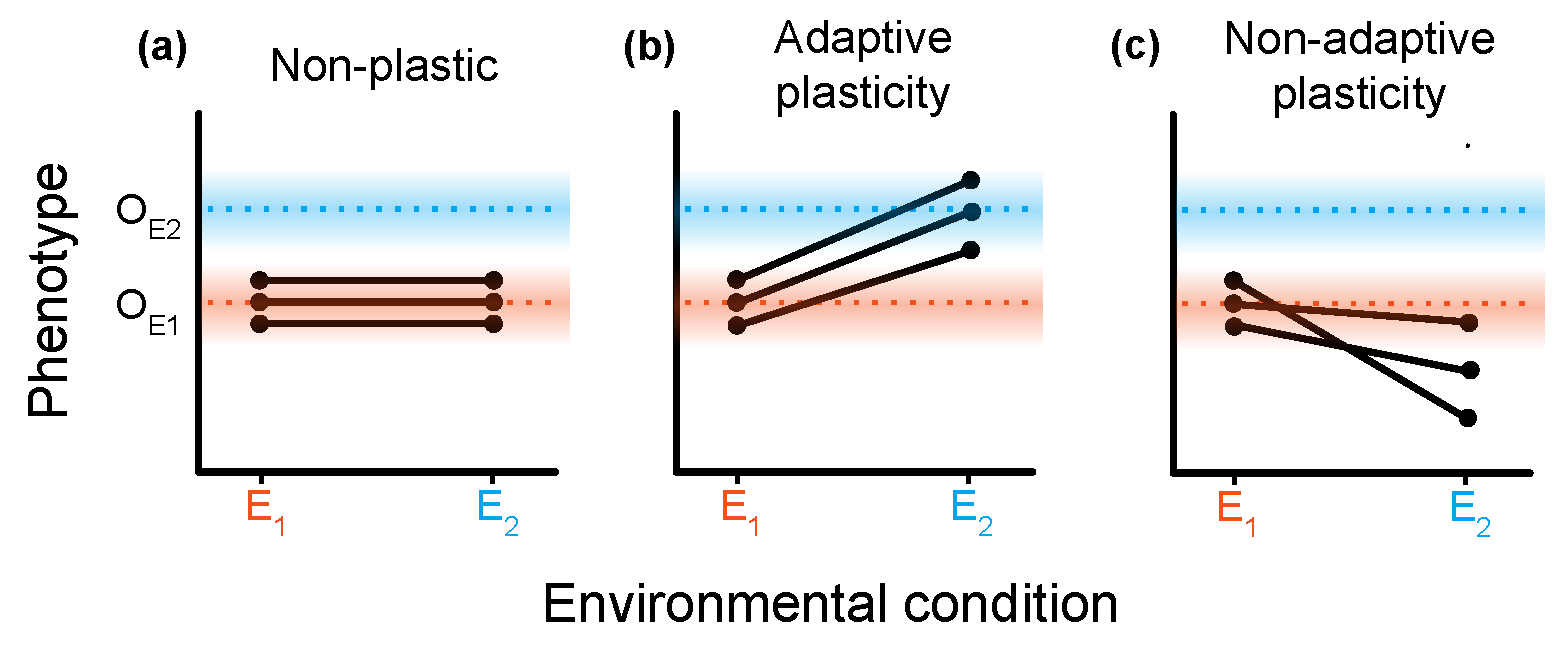
\includegraphics[width=0.85\textwidth]{02_consequences_of_plasticity/media/media-reaction-norms.pdf}
\caption{\small
Hypothetical reaction norms for populations comprising genotypes placed in different environments.
A reaction norm describes phenotypic change (or lack thereof) induced by environmental variation~\citep{west-eberhard_phenotypic_2008}. 
In all panels, two environmental conditions (denoted E$_1$ and E$_2$) are shown on the x-axis.
The y-axis indicates the phenotype expressed in each environment with O$_{\text{E}1}$ and O$_{\text{E}2}$ designating the optimal phenotype for E$_1$ and E$_2$, respectively.
Each pair of points connected by a solid black line denotes a genotype, with the points themselves representing its hypothetical phenotypes in each environment.
We present three scenarios for how populations could respond to a change from E$_1$ to E$_2$.
(a) A non-plastic population where phenotypes do not change with environmental shifts.  
% In such cases, we would expect strong directional selection toward O$_{\text{E}2}$ after the environment changes.
(b) An adaptively plastic population where phenotypes dynamically adjust to the new optimum. 
% As such, we would expect this population to remain relatively stable after the environment changes.
% (c) A population exhibiting non-adaptive plasticity with substantial variation in how individuals respond to the environmental change. In this case, we expect the change in environment to result in a rapid evolutionary sweep by genotypes closest to the new optimal phenotype.
% (d) A population exhibiting maladaptive plasticity. 
(c) A population exhibiting non-adaptive plasticity where environmental change induces phenotypes further away from the optimum. 
% relative to the given environmental change. 
% When the environment changes, there is little variation for selection to act on, and without beneficial mutations, this population could be at risk of extinction.
}
\label{fig:reaction-norms}
\end{figure}

% -- Plasticity as a source of cryptic variation --
Phenotypic plasticity allows for the accumulation of genetic variation in genomic regions that are unexpressed under current environmental conditions.
Such cryptic (``hidden'') genetic variation can serve as a source of diversity in the population, upon which selection can act when the environment changes \citep{schlichting_hidden_2008,levis_evaluating_2016}.
It remains unclear to what extent and under what circumstances this cryptic variation caches adaptive potential or merely accumulates deleterious alleles \citep{gibson_uncovering_2004,paaby_cryptic_2014,zheng_cryptic_2019}.

% -- Genes as followers --
The ``genes as followers'' hypothesis (also known as the ``plasticity first'' hypothesis) predicts that phenotypic plasticity may facilitate adaptive evolutionary change by producing variants with enhanced fitness under stressful or novel conditions \citep{west-eberhard_developmental_2003,schwander_genes_2011,levis_evaluating_2016}.
Environmentally-induced trait changes can be refined through selection over time (\textit{i.e.}, genetic accommodation).
Further, selection may drive plastic phenotypes to lose their environmental dependence over time in a process known as genetic assimilation \citep{west-eberhard_developmental_2005,pigliucci_phenotypic_2006,crispo_baldwin_2007,schlichting_phenotypic_2014,levis_evaluating_2016}.
In this way, environmentally-induced phenotypic changes can precede an evolutionary response.

% -- Plastic rescue + wrap up on plasticity background? --
Phenotypic plasticity may also ``rescue'' populations from extinction under changing environmental conditions by buffering populations against novel stressors.
This buffer promotes stability and persistence and grants populations time to further adapt to rapidly changing environmental conditions \citep{west-eberhard_developmental_2003,chevin_when_2010}.

Disparate predictions about how phenotypic plasticity may shift the course of subsequent evolution are not necessarily mutually exclusive.
Genetic and environmental contexts determine if, and to what extent, phenotypic plasticity promotes or constrains subsequent evolution.
Figure~\ref{fig:reaction-norms} overviews how we might expect different forms of phenotypic plasticity to result in different evolutionary responses after an environmental change.
In Figure~\ref{fig:reaction-norms}a, we would expect non-plastic populations to experience strong directional selection toward the new optimum (O$_{\text{E}2}$) after the environment changes.
We would expect an adaptively plastic population (Figure~\ref{fig:reaction-norms}b) to remain relatively stable after the environment changes, as plasticity shifts organisms' phenotypes to the new optimum.
In Figure~\ref{fig:reaction-norms}c, we would expect the non-adaptively plastic population to experience strong directional selection on their response to the new environmental conditions; indeed, such maladaptive plasticity may even put the population at risk of extinction in the absence of beneficial mutations.

%%%%%%%%%%%%%%%%%%%%%%
% -- Digital evolution --
%%%%%%%%%%%%%%%%%%%%%%
Experimental studies investigating the relationship between phenotypic plasticity and evolutionary outcomes can be challenging to conduct in natural systems.
Such experiments would require the ability to irreversibly toggle plasticity followed by long periods of evolution during which detailed phenotypic data would need to be collected.
Digital evolution experiments have emerged as a powerful research framework from which evolution can be studied.
In digital evolution, self-replicating computer programs (digital organisms) compete for resources, mutate, and evolve following Darwinian dynamics  \citep{wilke_biology_2002}.
Digital evolution studies balance the speed and transparency of mathematical and computational simulations with the open-ended realism of laboratory experiments.
Modern computers allow us to observe many generations of digital evolution at tractable time scales; thousands of generations can take mere minutes as opposed to months, years, or millennia.
Digital evolution systems also allow for perfect, non-invasive data tracking.
Such transparency permits the tracking of complete evolutionary histories within an experiment, which circumvents the historical problem of drawing evolutionary inferences using incomplete records (from frozen samples or fossils) and extant genetic sequences.
Additionally, digital evolution systems allow for experimental manipulations and analyses that go beyond what is possible in wet-lab experiments.
Such analyses have included exhaustive knockouts of every site in a genome to identify the functionality of each \citep{lenski_evolutionary_2003},
comprehensive characterization of local mutational landscapes \citep{lenski_genome_1999,canino-koning_fluctuating_2019},
and the real-time reversion of all deleterious mutations as they occur to isolate their long-term effects on evolutionary outcomes \citep{covertiiiExperimentsRoleDeleterious2013}.
Furthermore, digital evolution studies allow us to directly toggle the possibility for adaptive plastic responses to evolve, which enables us to empirically test hypotheses that were previously relegated to theoretical analyses.

%%%%%%%%%%%%%%%%%%%%%%
% -- Overview of what we're testing / doing --
%%%%%%%%%%%%%%%%%%%%%%

In this study, we conduct digital evolution experiments to investigate how the evolution of adaptive phenotypic plasticity shifts the course of evolution in a cyclically changing environment.
We use the Avida Digital Evolution Platform \citep{ofria_avida:_2009}.
Avida is an open-source system that has been used to conduct a wide range of well-regarded studies on evolutionary dynamics, including
the origins of complex features \citep{lenski_evolutionary_2003},
the survival of the flattest effect \citep{wilke_evolution_2001},
and the origins of reproductive division of labor \citep{goldsby_evolutionary_2014}.
Our experiments build directly on previous studies in Avida that characterized the \textit{de novo} evolution of adaptive phenotypic plasticity \citep{clune_investigating_2007,lalejini_evolutionary_2016} as well as previous work investigating the evolutionary consequences of fluctuating environments for populations of non-plastic digital organisms \citep{li_digital_2004,canino-koning_fluctuating_2019}.
Of particular relevance, \cite{clune_investigating_2007} and \cite{lalejini_evolutionary_2016} experimentally demonstrated that adaptive phenotypic plasticity can evolve given the following four conditions (as described by \citealt{ghalambor_behavior_2010}):
(1) populations experience temporal environmental variation,
(2) these environments are differentiable by reliable cues,
(3) each environment favors different phenotypic traits,
and (4) no single phenotype exhibits high fitness across all environments.
We build on this previous work, but we shift our focus from the evolutionary causes of adaptive phenotypic plasticity to investigate its evolutionary consequences in a fluctuating environment.
Specifically, we examine the effects of adaptive plasticity on subsequent genomic and phenotypic change, the capacity to evolve and then maintain novel traits, and the accumulation of deleterious alleles.

% - what we did -
Each of our experiments are divided into two phases: in phase one, we precondition sets of founder organisms with differing plastic or non-plastic adaptations;
in phase two, we examine the subsequent evolution of populations founded with organisms from phase one under specific environmental conditions (Figure \ref{fig:experimental-design}).
First, we examine the evolutionary histories of phase two populations to test whether adaptive plasticity constrained subsequent genomic and phenotypic changes.
Next, we evaluate how adaptive plasticity influences how well populations produced by each type of founder can evolve and retain novel adaptive traits.
Finally, we examine lineages to determine whether adaptive plasticity facilitated the accumulation of cryptic genetic variation that would prove deleterious when the environment changed.

%%%%%%%%%%%%%%%%%%%%%%
% - Overview of findings -
%%%%%%%%%%%%%%%%%%%%%%
We found that the evolution of adaptive plasticity reduced subsequent rates of evolutionary change in a cyclic environment.
The non-plastic populations underwent more frequent selective sweeps and accumulated many more genetic changes over time, as non-plastic populations relied on genetic variation from \textit{de novo} mutations to continuously readapt to environmental changes.
The evolution of adaptive phenotypic plasticity buffered populations against environmental fluctuations, whereas repeated selective sweeps in non-plastic populations drove the accumulation of deleterious mutations and the loss of secondary beneficial traits. % via deleterious hitchhiking.
As such, adaptively plastic populations were better able to retain novel traits than their non-plastic counterparts.
In general, the evolution of adaptive phenotypic plasticity shifted evolutionary dynamics to be more similar to that of populations evolving in a static environment than to non-plastic populations evolving in an identical fluctuating environment.

\section{Materials and Methods}
\label{sec:methods}

\subsection{The Avida Digital Evolution Platform}
\label{sec:methods:avida}

% -- Define digital organisms --
Avida is a study system wherein self-replicating computer programs (digital organisms) compete for space on a finite toroidal grid \citep{ofria_avida:_2009}.
Each digital organism is defined by a linear sequence of program instructions (its genome) and a set of virtual hardware components used to interpret and express those instructions.
Genomes are expressed sequentially except when the execution of one instruction (\textit{e.g.}, a ``jump'' instruction) deterministically changes which instruction should be executed next.
Genomes are built using an instruction set that is both robust (\textit{i.e.}, any ordering of instructions is syntactically valid, though not necessarily meaningful) and Turing Complete (\textit{i.e.}, able to represent any computable function, though not necessarily in an efficient manner).
The instruction set includes operations for basic computations, flow control (\textit{e.g.}, conditional logic and looping), input, output, and self-replication.
% The virtual hardware set includes components such as a central processing unit (CPU) for executing instructions, registers to store values, buffers for inputs and outputs, and memory stacks \citep{ofria_avida:_2009}.

% -- Define reproduction & mutation --
Organisms in Avida reproduce asexually by copying their genome instruction-by-instruction and then dividing.
However, copy operations are imperfect and can result in single-instruction substitution mutations in an offspring's genome.
For this work, we configured copy operations to err at a rate of one expected mutation for every 400 instructions copied (\textit{i.e.}, a per-instruction error rate of 0.0025).
We held individual genomes at a fixed length of 100 instructions (the default genome size in Avida); that is, we did not include insertion and deletion mutations.
We used fixed-length genomes to control for treatment-specific conditions resulting in the evolution of substantially different genome sizes \citep{supplemental_material}\footnote{
We repeated our experiments without genome size restrictions and observed qualitatively similar results (see supplemental material, \citealt{supplemental_material}).
}, which could, on its own, drive differences in evolutionary outcomes among experimental treatments.
When an organism divides in Avida, its offspring is placed in a random location on the toroidal grid, replacing any previous occupant.
For this work, we used the default 60 by 60 grid size, which limits the maximum population size to 3600 organisms.
As such, improvements to the speed of self-replication are advantageous in the competition for space.

% -- Define fitness/metabolic rate/improving replication speed --
During evolution, organism replication rates improve in two ways: by improving genome efficiency (\textit{e.g.}, using a more compact encoding) or by accelerating the rate at which the genome is expressed (their ``metabolic rate'').
An organism's metabolic rate determines the speed at which it executes instructions in its genome.
Initially, an organism's metabolic rate is proportional to the length of its genome, but that rate is adjusted as it completes designated functions, such as performing Boolean logic functions \citep{ofria_avida:_2009}.
In this way, we can reward or punish particular phenotypic traits (\textit{i.e.}, Boolean logic functions).

\subsubsection{Phenotypic plasticity in Avida}
\label{sec:methods:avida:plasticity}

% -- Phenotypes & Phenotypic plasticity --
%   - What is a phenotype in Avida?
In this work, we measure a digital organism's phenotype as the set of Boolean logic functions that it performs (\textit{i.e.} expresses) in a given environment.
Sensory instructions in the Avida instruction set allow organisms to detect how performing a particular function would affect their metabolic rate (see supplemental material for more details, \citealt{supplemental_material}).
We define a phenotypically plastic organism as one that uses sensory information to alter which functions it performs based on the environment.

% -- Adaptive plasticity & non-adaptive plasticity --
Phenotypic plasticity in Avida can be adaptive or non-adaptive for a given set of environments.
Adaptive plasticity shifts net function expression closer to the optimum for the given environments.
Non-adaptive plasticity changes function expression in either a neutral or deleterious way.
In this work, optimal plasticity toggles functions to always perfectly match the set of rewarded functions for the given set of environments.

\subsection{Experimental design}
\label{sec:methods:experiment}

\begin{figure}[h!]
  \centering
  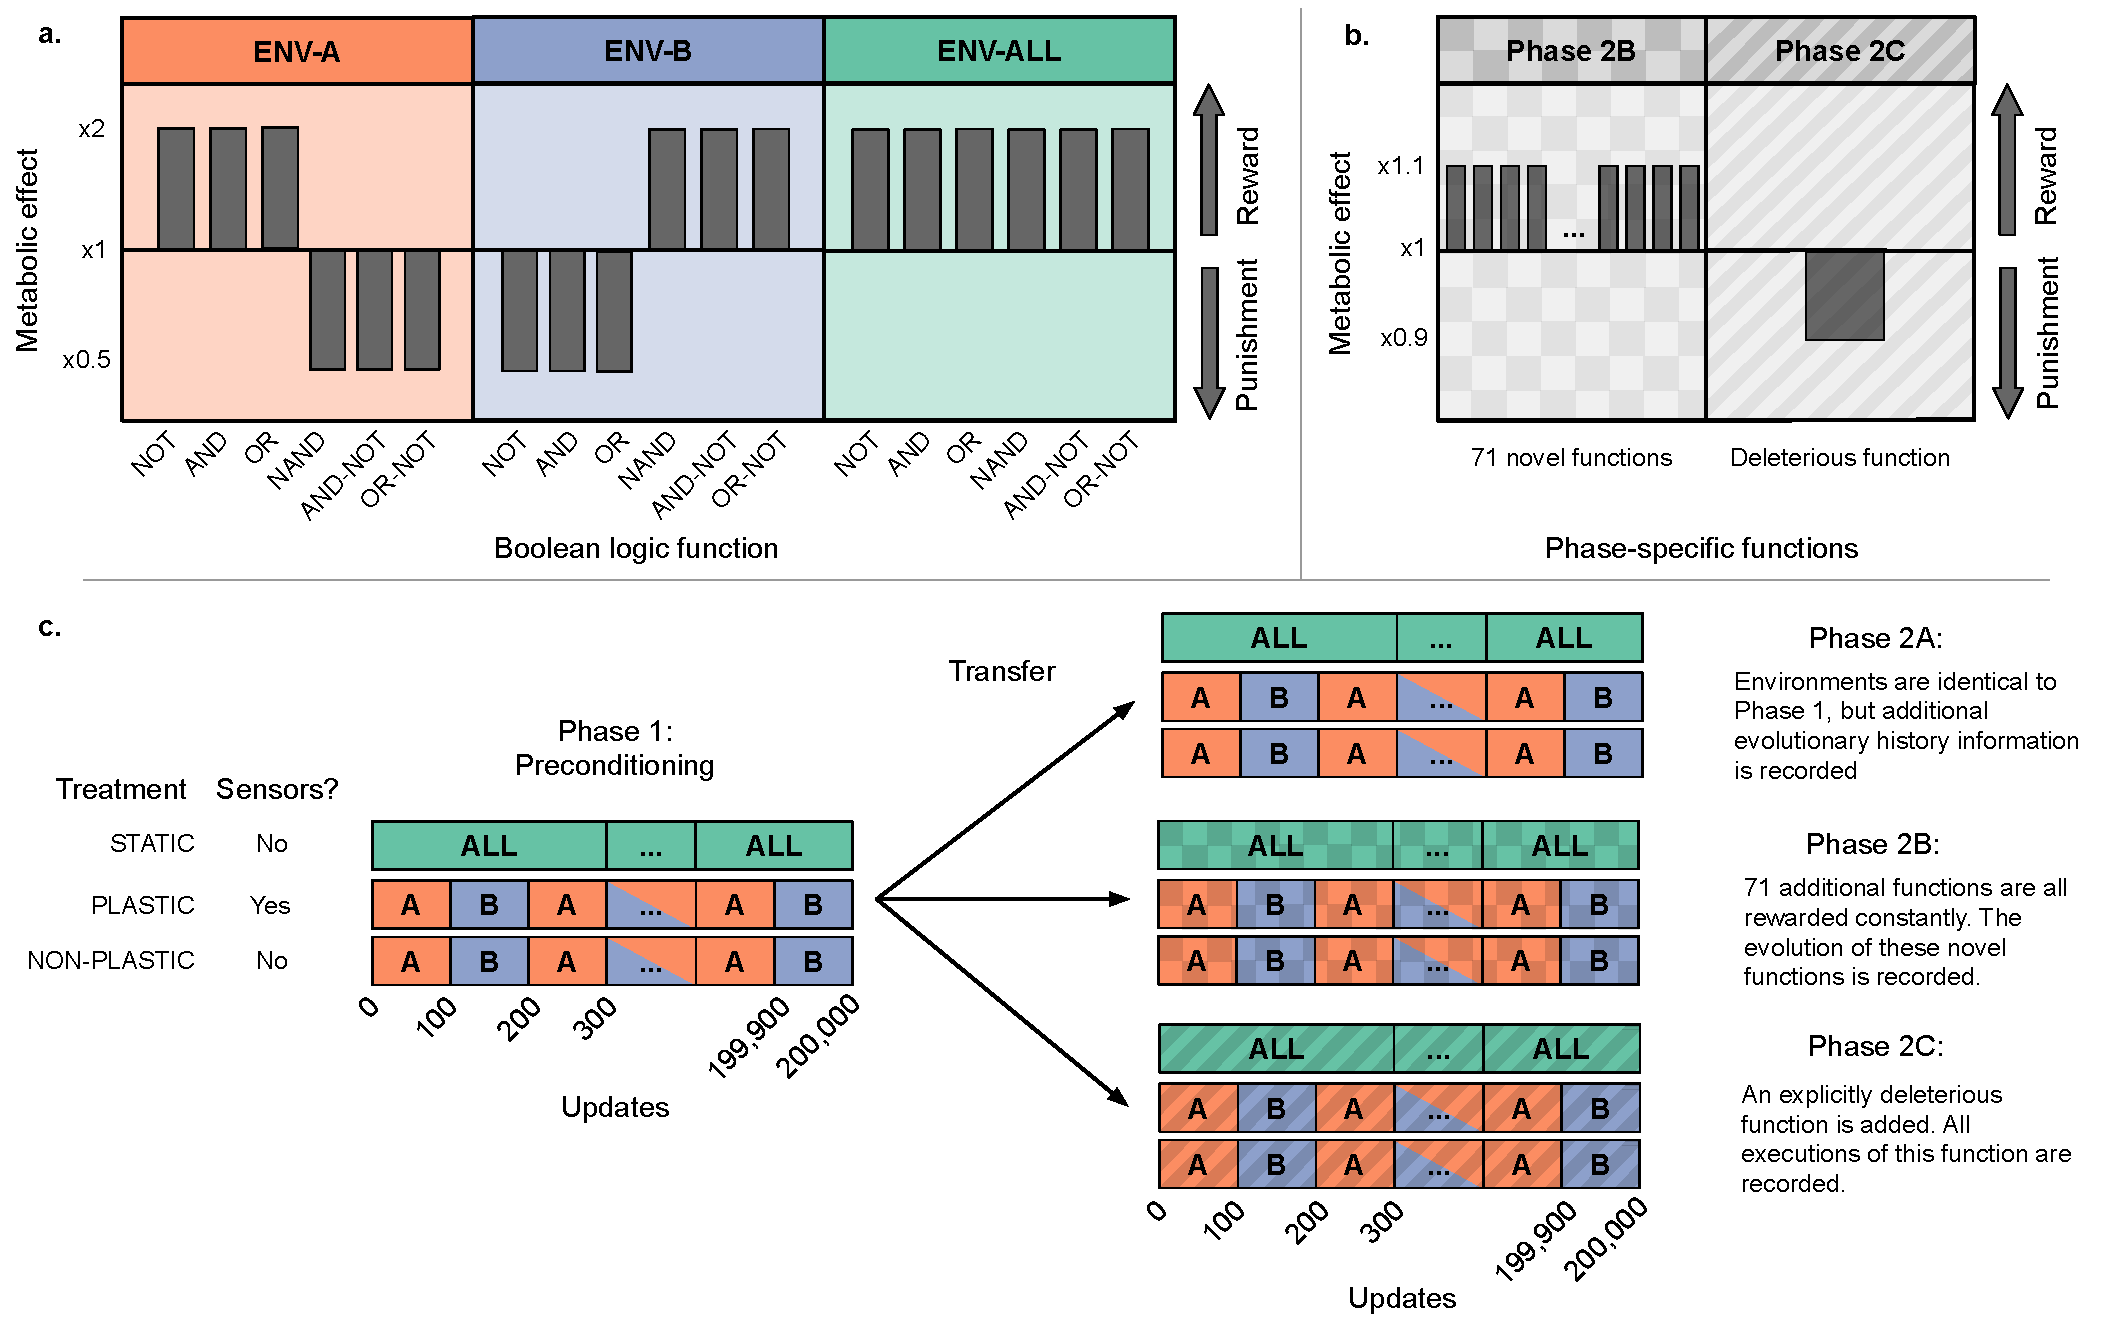
\includegraphics[width=1\textwidth]{02_consequences_of_plasticity/media/media-experimental-design.pdf}
  \caption{\small
  The three plots in panel (a) show the environmental conditions used in every experiment and whether they reward or punish each base function.
  The two plots in (b) show the additional functions added in phases 2B and 2C. %Optional: phase 2A is not shown as it adds no additional functions
  %All novel tasks in phase 2B confer a 10\% metabolic reward, while executing the poisonous task in phase 2C causes a 10\% metabolic punishment (bars not drawn to scale).
  Panel (c) shows treatment differences and experimental phases.
  Treatments are listed on the left, with each treatment specifying its environmental configuration and whether sensors are functional.
  We conducted three independent two-phase experiments, each described on the right.
  Phases 2B and 2C are textured to match their function definitions in panel (b).
  Phase one is repeated for \textit{each} experiment with 100 replicate populations per treatment per experiment.
  For each replicate at the end of phase one, we used an organism of the most abundant genotype to found the second phase population.
  All STATIC and NON-PLASTIC populations move on to phase two, but PLASTIC populations only continue to the second phase if their most abundant genotype exhibits optimal plasticity.
  Metrics are recorded only in phase two.
  }
  \label{fig:experimental-design}
\end{figure}

%%%%%%%%%%%%%%%%%%%%%%%%%%%%%%%%%%%%%%%%%%%%%%%%%
% OUTLINE
%%%%%%%%%%%%%%%%%%%%%%%%%%%%%%%%%%%%%%%%%%%%%%%%%
% Overview of experimental design - with diagram (not a subsubsection?)
% - Focused around diagram
% Environment implementations
% Specifications for Phase 1
% specifications for Phase 2A
% specifications for Phase 2B
% specifications for Phase 2C
%%%%%%%%%%%%%%%%%%%%%%%%%%%%%%%%%%%%%%%%%%%%%%%%%

% -- Treatments --
We conducted three independent experiments using Avida to investigate how the evolution of adaptive plasticity influences evolutionary outcomes in fluctuating environments.
For each experiment, we compared the evolutionary outcomes of populations evolved under three treatments (Figure \ref{fig:experimental-design}):
(1) a \textbf{PLASTIC} treatment where the environment fluctuates, and digital organisms can use sensory instructions to differentiate between environmental states;
(2) a \textbf{NON-PLASTIC} treatment with identical environment fluctuations, but where sensory instructions are disabled;
and (3) a \textbf{STATIC} control where organisms evolve in a constant environment.

% -- Experiment phases --
Each experiment was divided into two phases that each lasted for 200,000 updates\footnote{
    One update in Avida is the amount of time required for the average organism to execute 30 instructions.
    See \citep{ofria_avida:_2009} for more details.
} of evolution (Figure~\ref{fig:experimental-design}), which is equivalent to approximately 30,000 to 40,000 generations.
% Phase one of each experiment was an acclimation phase.
In phase one of each experiment, we evolved plastic, non-plastic, and control organisms for use in phase two.
In phase two, we founded new populations with these evolved organisms and examined their subsequent evolution under given combinations of treatment and experimental conditions.
During phase two, we tracked and saved each population's evolutionary history as well as saving the full final population.
Phase one was for preconditioning only; all comparisons between treatments were performed on phase two data.

\subsubsection{Environments}
\label{sec:methods:experiment:environments}

% ----- ENVIRONMENTS -----
% traits_set_a <- c("not", "and", "or")
% traits_set_b <- c("nand", "ornot", "andnot")

% -- Environment definitions --
% In all of our experiments, populations evolve in either static or fluctuating environments.

We constructed three experimental environmental conditions, abbreviated hereafter as ``ENV-A'', ``ENV-B'', and ``ENV-ALL''.
In ENV-A, organisms are rewarded for expressing the NOT, AND, and OR Boolean logic functions, and organisms are punished for expressing the NAND, AND-NOT, and OR-NOT functions. 
ENV-B is the reverse of ENV-A; that is, in ENV-B, organisms are rewarded for expressing the NAND, AND-NOT, and OR-NOT functions and are punished for expressing the NOT, AND, and OR functions.
In ENV-ALL, organisms are rewarded for expressing each of the NOT, AND, OR, NAND, AND-NOT, and OR-NOT functions.
In all environmental conditions (ENV-A, ENV-B, and ENV-ALL), a rewarded function expressed by an organism doubles their metabolic rate, allowing them to execute twice as many instructions in the same amount of time.
A punished function halves an organism's metabolic rate.
Each Boolean logic function is a non-trivial trait to evolve, as they each require the coordination of multiple genetic instructions to express~\citep{lenski_evolutionary_2003}.

% Figure \ref{fig:experimental-design} describes these environments based on whether each of six Boolean logic tasks (NOT, NAND, AND, OR-NOT, OR, and AND-NOT) is rewarded or punished.

% -- Treatment-specific environment details --
In both the PLASTIC and NON-PLASTIC treatments, the environment cycles between equal-length periods of ENV-A and ENV-B.
Each of these periods persist for 100 updates (approximately 15 to 20 generations).
Thus, populations experience a total of 1,000 full periods of ENV-A interlaced with 1,000 full periods of ENV-B during each experimental phase.
Previous work has shown that this rate of change reliably allows for the evolution of adaptive phenotypic plasticity in Avida~\citep{clune_investigating_2007,lalejini_evolutionary_2016}.

% -- Sensory instructions + control flow and controlling the capacity for plasticity --
Organisms in the PLASTIC treatments differentiate between ENV-A and ENV-B by executing one of six sensory instructions, each associated with a particular Boolean logic function; these sensory instructions detect whether their associated function is currently rewarded or punished.
By using sensory information in combination with execution flow-control instructions, organisms can conditionally perform different functions depending on the current environmental conditions.

\subsubsection{Experiment Phase 1 -- Environment preconditioning}
\label{sec:methods:experiment:phase-one}

For each treatment, we founded 100 independent populations from a common ancestral strain capable only of self-replication.
At the end of phase one, we identified the most abundant (\textit{i.e.}, dominant) genotype and sampled an organism with that genotype from each replicate population to found a new population for phase two.

For the PLASTIC treatment, we needed to ensure that our observations during the second phase of each experiment reflected the evolutionary consequences of adaptive plasticity. 
To do so, measured the plasticity of each PLASTIC-treatment population's dominant genotype by independently testing that genotype in each of ENV-A and ENV-B and recording the phenotype expressed in each environment.
We discarded PLASTIC-treatment phase one populations if the dominant genotype did not exhibit optimal plasticity (as defined in Section~\ref{sec:methods:avida:plasticity}), which ensured that PLASTIC-treatment phase two populations were founded with an optimally plastic organism.

% For the PLASTIC treatment, we measure the plasticity of each population's dominant genotype by independently testing the given genotype in each of ENV-A and ENV-B and recording the phenotype expressed in each environment.
% We discard PLASTIC-treatment phase one populations if the dominant genotype does not exhibit optimal plasticity (as defined in Section \ref{sec:methods:avida:plasticity}).
% This approach ensures that measurements taken on PLASTIC-treatment populations during the second phase of each experiment reflect the evolutionary consequences of adaptive plasticity.

\subsubsection{Experiment Phase 2A -- Evolutionary change rate}
\label{sec:methods:exp:evolutionary-change-rate}

We conducted experiment phase 2A to test for differences in evolutionary change---the accumulation of genetic and phenotypic changes---among populations evolving under each of our three treatment conditions (PLASTIC, NON-PLASTIC, and STATIC). 
Phase 2A continued exactly as phase one, except we tracked the rates of evolutionary change in each of the PLASTIC-, NON-PLASTIC-, and STATIC-treatment populations.
Specifically, we quantified evolutionary change using four metrics (each described in Table~\ref{tab:metrics-definitions}):
(1) coalescence event count,
(2) mutation count,
(3) phenotypic volatility,
and (4) mutational robustness.

While environmental conditions during phases one and 2A are identical, these phases are distinct in how populations are founded: each phase one population is founded with a common ancestor capable only of self-replication, whereas each phase two population is founded with an organism that was evolved in its treatment-specific conditions.
Thus, during phase two, phylogenies are rooted with an ancestor that is well-adapted to its treatment conditions, which, in turn, ensures that our observations can exclude dynamics associated with initial adaptation.

\subsubsection{Experiment Phase 2B -- Novel function evolution}
\label{sec:methods:exp:novel-task-evolution}

We conducted experiment phase 2B to quantify the extent to which organisms evolved under PLASTIC-, NON-PLASTIC-, and STATIC-treatment conditions were able to acquire and retain novel functions. 
Phase 2B extended the conditions of phase one by adding 71 novel Boolean logic functions~\citep{ofria_avida:_2009}, which were always rewarded in all treatments.
The original six phase one functions (NOT, NAND, AND, OR-NOT, OR, and AND-NOT; hereafter called ``base'' functions) continued to be rewarded or punished according to the particular treatment conditions.
% @CAO: line below can be restored (and reworded) if readers need help with the intuition.
%As such, in fluctuating environments, the six base tasks continued to fluctuate, but the additional 71 tasks were always rewarded; in static environments, performing any of the 77 logic tasks was always beneficial.
An organism's metabolic rate was increased by \novelTraitsReward\ for each novel function that it expressed (limited to one reward per function).
This reward provided a selective pressure to evolve these functions, but their benefits did not overwhelm the 100\% metabolic rate increase conferred by rewarded base functions.
As such, populations in the PLASTIC and NON-PLASTIC treatments could not easily escape environmental fluctuations by abandoning the fluctuating base functions.

During this experiment, we used three metrics to quantify novel function acquisition and retention in evolving populations (each described in Table~\ref{tab:metrics-definitions}):
% During this experiment, we tracked the extent to which populations evolving under each treatment were capable of acquiring and retaining novel tasks.
% Specifically, we used three metrics (each described in Table~\ref{tab:metrics-definitions}):
(1) final novel function count,
(2) novel function discovery,
and (3) novel function loss.

\subsubsection{Experiment Phase 2C -- Deleterious instruction accumulation}
\label{sec:methods:exp:deleterious-instruction-accumulation}

We conducted experiment phase 2C to quantify the extent to which organisms evolved under PLASTIC-, NON-PLASTIC-, and STATIC-treatment conditions acquired deleterious instructions via mutation.
Phase 2C extended the instruction set of phase one with a \code{deleterious} instruction.
When an organism executes a \code{deleterious} instruction, it performs a ``deleterious'' function, which reduces the organism's metabolic rate (and thus reproductive success) but does not otherwise alter the organism's behavior.
We imposed a 10\% penalty each time an organism performed the deleterious function, making the \code{deleterious} instruction explicitly harmful to execute.
We did not limit the number of times that an organism could perform the deleterious function, and as such, organisms could perform the deleterious function as many times as they executed the \code{deleterious} instruction.

We tracked the number of times each organism along the dominant lineage performed the deleterious function.
Specifically, we used two metrics (each described in Table~\ref{tab:metrics-definitions}):
(1) final deleterious function count and (2) deleterious function acquisition count.

\subsection{Experimental analyses}

%\newcommand*{\theadalt}[1]{\multicolumn{1}{c}{\bfseries #1}}

\setlength{\tabcolsep}{16pt}
\renewcommand{\arraystretch}{1.5}
\begin{table}[ht]
    \centering

    %\rowcolors{2}{gray!25}{white}
    \begin{tabularx}{\linewidth}{lX} % p{10cm}
        \rowcolor{gray!50}
        \hline
        \theadalt{Metric} & \theadalt{Description}   \\
        \hline
        \rowcolor{gray!25}
        \SweepsMetricName & \SweepsMetricDesc \\
        \rowcolor{white}
        \MutationCountMetricName & \MutationCountMetricDesc \\
        \rowcolor{gray!25}
        \PhenotypicVolatilityMetricName & \PhenotypicVolatilityMetricDesc \\
        \rowcolor{white}
        \MutationalStabilityMetricName & \MutationalStabilityMetricDesc \\
        \rowcolor{gray!25}
        \TaskPerformanceMetricName & \TaskPerformanceMetricDesc \\
        \rowcolor{white}
        \TaskDiscoveryMetricName & \TaskDiscoveryMetricDesc \\
        \rowcolor{gray!25}
        \TaskLossMetricName & \TaskLossMetricDesc \\
        \rowcolor{white}
        \FinalPoisonMetricName & \FinalPoisonMetricDesc \\
        \rowcolor{gray!25}
        \LineagePoisonMetricName & \LineagePoisonMetricDesc \\
        \hline
    \end{tabularx}

    \caption{Metric descriptions.}
    \label{tab:metrics-definitions}
\end{table}


% naive environment = what organism experiencing
% alternative environment = what organism is not currently experiencing

% - How we extracted representative lineages -
For each of our experiments, we tracked and analyzed the phylogenetic histories of evolving populations during phase two and generated a set of summary statistics (Table~\ref{tab:metrics-definitions}).
For each phylogenetic history, we counted the number of times that the most recent common ancestor for the population shifted and used this value as the number of coalescence events.
Next, at the final time point, we identified the most abundant genotype in the evolved population, and chose a \textit{representative organism} from that genotype for further analysis.
% We then isolated the lineage from the founding organism to the representative organism, which we used as the representative lineage for further analysis.
% We used the lineage from the founding organism to the representative organism as the \textit{representative lineage} for further analysis.
We used the lineage from the founding organism to the representative organism to summarize the evolutionary pathway of a population. 
This lineage represents the majority of the evolutionary history from the given population as long as the entire population traces back to the lineage in recent history.
We manually inspected evolved phylogenies and found no evidence that any of our experimental treatments supported long-term coexistence.
As such, analyses of the representative lineages reflect the majority of evolutionary history for a given population.

% To be confident that each representative lineage reflected the majority of the evolutionary history from a given populuation at the end of the ex
% [These lineages represent the majority of the evolutionary history from a given population only if there aren't members of the population that haven't diverged too far in the past / only if single the entire population traces back to that lineage in recent history (i.e., no long-term coexistence)].
% We manually inspected evolved phylogenies and found no evidence that any of our experimental treatments supported long-term coexistence.
% As such, each of the representative lineages reflect the majority of evolutionary history from a given population at the end of our experiment.

% -- PHENOTYPIC PROFILE --
% DEFINE PHENOTYPIC PROFILE - metric definitions will use this.
Some of our metrics (Table \ref{tab:metrics-definitions}) required us to measure genotype-by-environment interactions.
Importantly, in the fluctuating environments, we needed to differentiate phenotypic changes that were caused by mutations from those that were caused by environmental changes.
To accomplish this, we produced organisms with the given focal genotype, measured their phenotype in each environmental condition, and aggregated the resulting phenotypes to create a \textit{phenotypic profile}.
Although organisms with different genotypes may express the same set of functions across environmental conditions, their phenotypic profiles may not necessarily be the same.
For example, an organism that expresses NOT in ENV-A and NAND in ENV-B has a distinct phenotypic profile from one that expresses NAND in ENV-A and NOT in ENV-B.
Because phenotypic profiles encapsulate function expression across all relevant environmental conditions (ENV-A and ENV-B), a change in phenotypic profile from parent to offspring indicates a mutationally-induced phenotypic change.  

% -- GENETIC MANIPULATION / MUTATIONAL NEIGHBORHOOD --
% How do we produce mutants for analyses?
While most analyses employed here are retrospective metrics applied to lineages, digital evolution allows precise manipulations on individual organisms and genomes.
Mutational robustness uses this technique when looking at the possible mutations on a representative genotype.
Genomes in Avida are linear sequences of instructions, and as such, possible mutations can be simulated by substituting other instructions at the desired site.
Indeed, the mutational robustness of a genotype examines all one-step mutations (\textit{i.e.}, each mutation where exactly one instruction is substituted).
This allows us to disentangle whether the frequency of mutationally-induced phenotypic changes observed along a lineage is a consequence of evolved genetic architectures versus the result of population dynamics that actively skewed the distribution of organisms along the lineage; that is, are genomes organized such that mutations are more likely to induce phenotypic changes, or are organisms with phenotypes different from their parents more likely to be successful and thus appear along the representative lineage?

% the results of the lineage metrics are a consequence of evolved genetic architectures versus ongoing population dynamics that are actively skewing the distribution of organisms along each lineage. %or the results of selection.
%otherwise.
%purely the results of selection.


\subsection{Statistical analyses}

Across all of our experiments, we differentiated between sample distributions using non-parametric statistical tests.
For each major analysis, we first performed a Kruskal-Wallis test \citep{kruskal_use_1952} to
determine if there were significant differences in results from the PLASTIC, NON-PLASTIC, and STATIC treatments (significance level $\alpha=0.05$).
If so, we applied a Wilcoxon rank-sum test \citep{kotz_individual_1992} to distinguish between pairs of treatments.
We applied Bonferroni corrections for multiple comparisons \citep{rice_analyzing_1989} where appropriate.

\subsection{Software availability}

We conducted our experiments using a modified version of the Avida software, which is open source and freely available on \href{https://github.com/amlalejini/evolutionary-consequences-of-plasticity}{GitHub}~\citep{supplemental_material}.
Modifications to Avida included an improved phylogeny tracking system that enabled us to track coalescence events and the addition of custom sensory instructions specific to our experiments.
We used Python for data processing, and we conducted all statistical analyses using R version 4~\citep{r_core_team_r_v4}.
We used the tidyverse collection of R packages~\citep{r_tidyverse_2019} to wrangle data, and we used the following R packages for analysis, graphing, and visualization:
ggplot2~\citep{R-ggplot2},
cowplot~\citep{R-cowplot},
Color Brewer~\citep{harrower_colorbrewerorg_2003,R-Brewer_2014},
rstatix~\citep{R-rstatix},
ggsignif~\citep{R-ggsignif},
scales~\citep{R-scales},
Hmisc~\citep{harrelljrHmiscHarrellMiscellaneous2020},
fmsb~\citep{R-fmsb},
and boot~\citep{R-boot}.
We used R markdown~\citep{rmarkdown} and bookdown~\citep{R-bookdown} to generate web-enabled supplemental material.
All of the source code for our experiments and analyses, including configuration files and guides for replication, can be found in our supplemental material, which is hosted on \href{https://github.com/amlalejini/evolutionary-consequences-of-plasticity}{GitHub}~\citep{supplemental_material}.
Additionally, our experimental data is available on the Open Science Framework at \url{https://osf.io/sav2c/} \citep{osf_data}.

%%%%%%%%%%%%%%%%%%%%%%%%%%%%%%%%%%%%%%%%%%%%%%%%%%%%%%%%%%%%
% INSTRUCTIONS:
% This section may be divided by subheadings. Footnotes should not be used and must be transferred to the main text.
%%%%%%%%%%%%%%%%%%%%%%%%%%%%%%%%%%%%%%%%%%%%%%%%%%%%%%%%%%%%

\section{Results}

\subsection{Adaptive phenotypic plasticity slows evolutionary change in fluctuating environments}

\begin{figure}[h!]
  \centering
  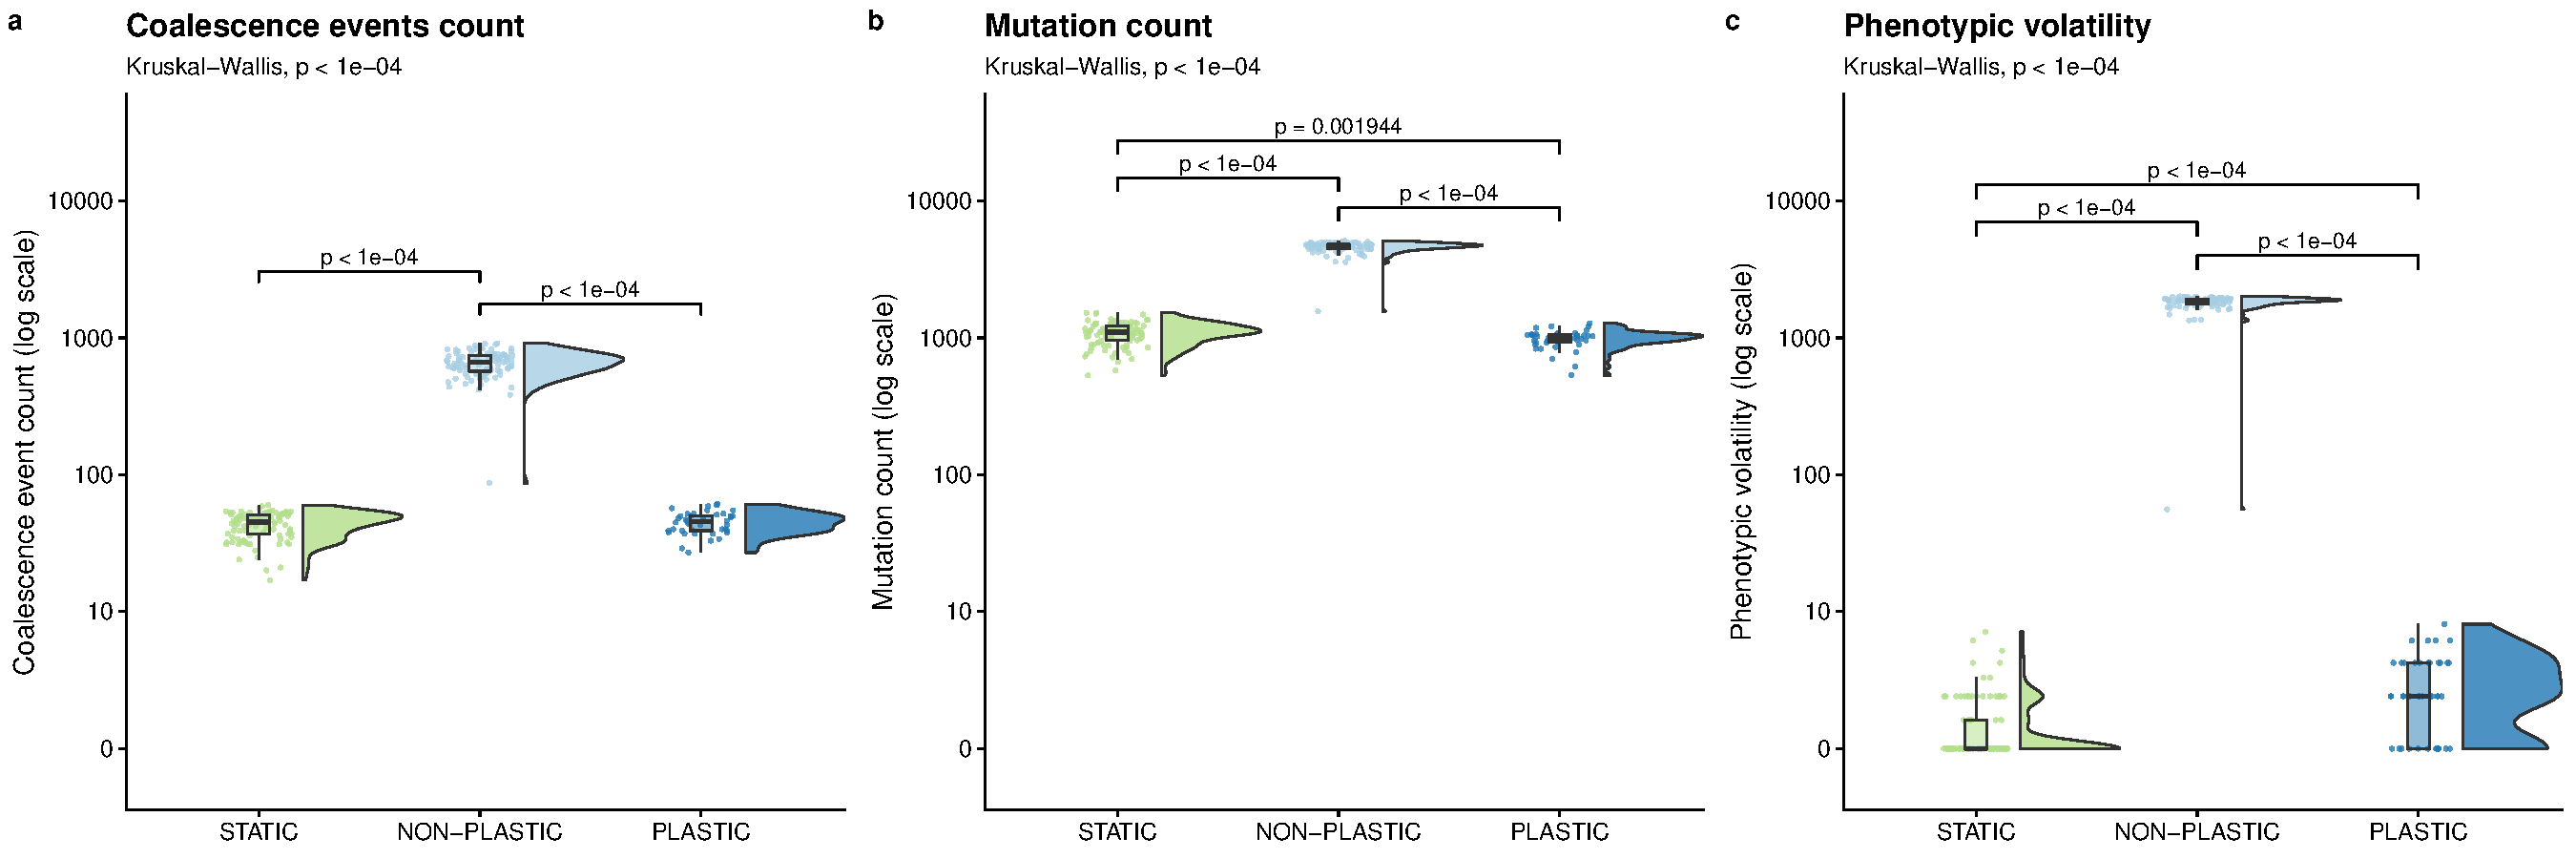
\includegraphics[width=1\textwidth]{02_consequences_of_plasticity/media/media-evolutionary-change-magnitude-panel.pdf}
  \caption{\small
  Raincloud plots~\citep{allen_raincloud_2019} of
  (a) coalescence event count,
  (b) mutation count,
  and (c) phenotypic volatility.
  See Table~\ref{tab:metrics-definitions} for descriptions of each metric.
  Each plot is annotated with statistically significant comparisons (Bonferroni-corrected pairwise Wilcoxon rank-sum tests).
  Note that adaptive phenotypic plasticity evolved in \evolutionaryChangeRatePlasticReps\ of \evolutionaryChangeRateReplicates\ replicates from the PLASTIC treatment during phase one of this experiment; we used this more limited group to found \evolutionaryChangeRatePlasticReps\ phase-two PLASTIC replicates from which we report these PLASTIC data.
  }
  \label{fig:evolutionary-dynamics-magnitude}
\end{figure}


%%%%%%%%%%%%%%%%%%%%%%%%%%%%%%%%%
% Results to report (2021-02-08 experiment)
% ----- GENERATIONS -----
% - average generations elapsed (of a population)
%   - NON-PLASTIC (median: 41768.65) > PLASTIC (median: 31697.65) > STATIC (median: 30839.75)
%   condition     mean    sd
%   <chr>        <dbl> <dbl>
% 1 NON-PLASTIC 41090. 2702.
% 2 PLASTIC     31016. 2615.
% 3 STATIC      30002. 3011.

%
% ----- SWEEPS -----
% - coalescence events (total)
%   - NON-PLASTIC (median: 663.5) > ( PLASTIC (median: 45.5) ~~ STATIC (median: 45) )
% - Average number of generations between coalescence events (gens / sweeps)
%   - ( PLASTIC (median: 685.001780758557) ~~ STATIC (median: 693.676265008576) ) > NON-PLASTIC (median: 62.0184902295191)
%
% ----- PHENOTYPIC VOLATILITY -----
% - phenotypic volatility (total)
%   - i.e., total number of times phenotypes change along lineages
%   - NON-PLASTIC (median: 1868) > PLASTIC (median: 2) > STATIC (median: 0)
% - phenotypic volatility / lineage length
%   - i.e., how often do genomic changes reflect changes in phenotype?
%   - NON-PLASTIC (median: 0.437) > PLASTIC (median: 0.0022) > STATIC (median: 0)
% - phenotypic volatility / generations
%   - i.e., per-offspring rate of phenotypic changes
%   - NON-PLASTIC (median: 0.0447) > PLASTIC (median: 6.33e-05) > STATIC (median: 0)
%
% ----- MUTATION ACCUMULATION -----
% - mutation accumulation (total)
%   - NON-PLASTIC (median: 4657.5) > STATIC (median: 1100) > PLASTIC (median: 998.5)
% - mutation accumulation / lineage length
%   - NON-PLASTIC (median: 1.10048311715591) > STATIC (median: 1.03794597464116) > PLASTIC (median: 1.0328599144651)
% - mutation accumulation / generation
%   - NON-PLASTIC (median: 0.11) > STATIC (median: 0.0368) > PLASTIC (median: 0.0319)
%
% ----- MUTATIONAL EFFECTS -----
% - fraction of mutational steps that alter (aggregate) phenotype
%   - NON-PLASTIC (mean: 0.434007, CI [0.4242,  0.4406]) > PLASTIC (mean: 0.002717008, 0.0020,  0.0035) > STATIC (mean: 0.0006788834, CI [0.0004,  0.0009])
% - fraction of phenotype-altering mutation steps that alter unexpressed phenotype (PLASTIC condition only)
%   - mean: 0.8247126 CI [0.7443,  0.8994]
% - fraction of mutations that affect unexpressed phenotype that are deleterious (PLASTIC only)
%   - mean: 0.5172414 CI [0.4402,  0.5977]
% - fraction of mutations that affect unexpressed phenotype that are beneficial (PLASTIC only)
%   - mean: 0.4827586 CI [0.4046,  0.5598]
%%%%%%%%%%%%%%%%%%%%%%%%%%%%%%%%%

% -- Magnitude of evolutionary change --
%  - Selective sweeps
%  - Mutation accumulation
%  - Phenotypic volatility
In experimental phase 2A,
we tested whether adaptive phenotypic plasticity constrained or promoted subsequent evolutionary change in a fluctuating environment.
First, we compared the total amount of evolutionary change in populations evolved under the PLASTIC, NON-PLASTIC, and STATIC treatments as measured by coalescence event count, mutation count, and phenotypic volatility (Figure~\ref{fig:evolutionary-dynamics-magnitude}).
According to each of these metrics, NON-PLASTIC populations experienced a larger magnitude of evolutionary change than either PLASTIC or STATIC populations.
We observed significantly higher coalescence event counts in NON-PLASTIC populations than in PLASTIC or STATIC populations (Figure~\ref{fig:evolutionary-dynamics-magnitude}\hyperref[fig:evolutionary-dynamics-magnitude]{a}).
NON-PLASTIC lineages had significantly higher mutation counts (Figure~\ref{fig:evolutionary-dynamics-magnitude}b) and phenotypic volatility than PLASTIC or STATIC lineages (Figure~\ref{fig:evolutionary-dynamics-magnitude}c).

% -- Elapsed generations --
Changing environments have been shown to increase generational turnover (\textit{i.e.}, how rapidly generations elapse) in Avida populations~\citep{canino-koning_evolution_2016}, which could explain why we observe a larger magnitude of evolutionary change at the end of 200,000 updates of evolution in NON-PLASTIC populations.
Indeed, we found that significantly more generations of evolution elapsed in NON-PLASTIC populations (mean of $41090\pm2702$ std. dev.) than in PLASTIC (mean of $31016\pm2615$ std. dev.) or STATIC (mean of $30002\pm3011$ std. dev.) populations during phase 2A (corrected Wilcoxon rank-sum tests, p $<10^{-4}$).

% -- Rate of evolutionary change => intuition --
To evaluate whether increased generational turnover explains the greater magnitude of evolutionary change in NON-PLASTIC populations, we examined the average number of generations between coalescence events and the realized mutational robustness of lineages (Table \ref{tab:metrics-definitions}).
A coalescence event indicates a selective sweep, which is a hallmark of adaptive evolutionary change.
Realized mutational robustness measures the frequency that mutations cause phenotypic changes along a lineage.
We expect that static conditions should favor fit lineages with high realized mutational robustness that no longer undergo rapid adaptive change and hence do not trigger frequent coalescence events.
Under fluctuating conditions, however, lineages must be composed of plastic organisms if they are to maintain both high fitness and realized mutational robustness.
Without plasticity, we expect fluctuating conditions to produce lineages with low realized mutational robustness and frequent coalescence events as populations must continually acquire and fix mutations to readapt to the environment.

\begin{figure}[h!]
  \centering
  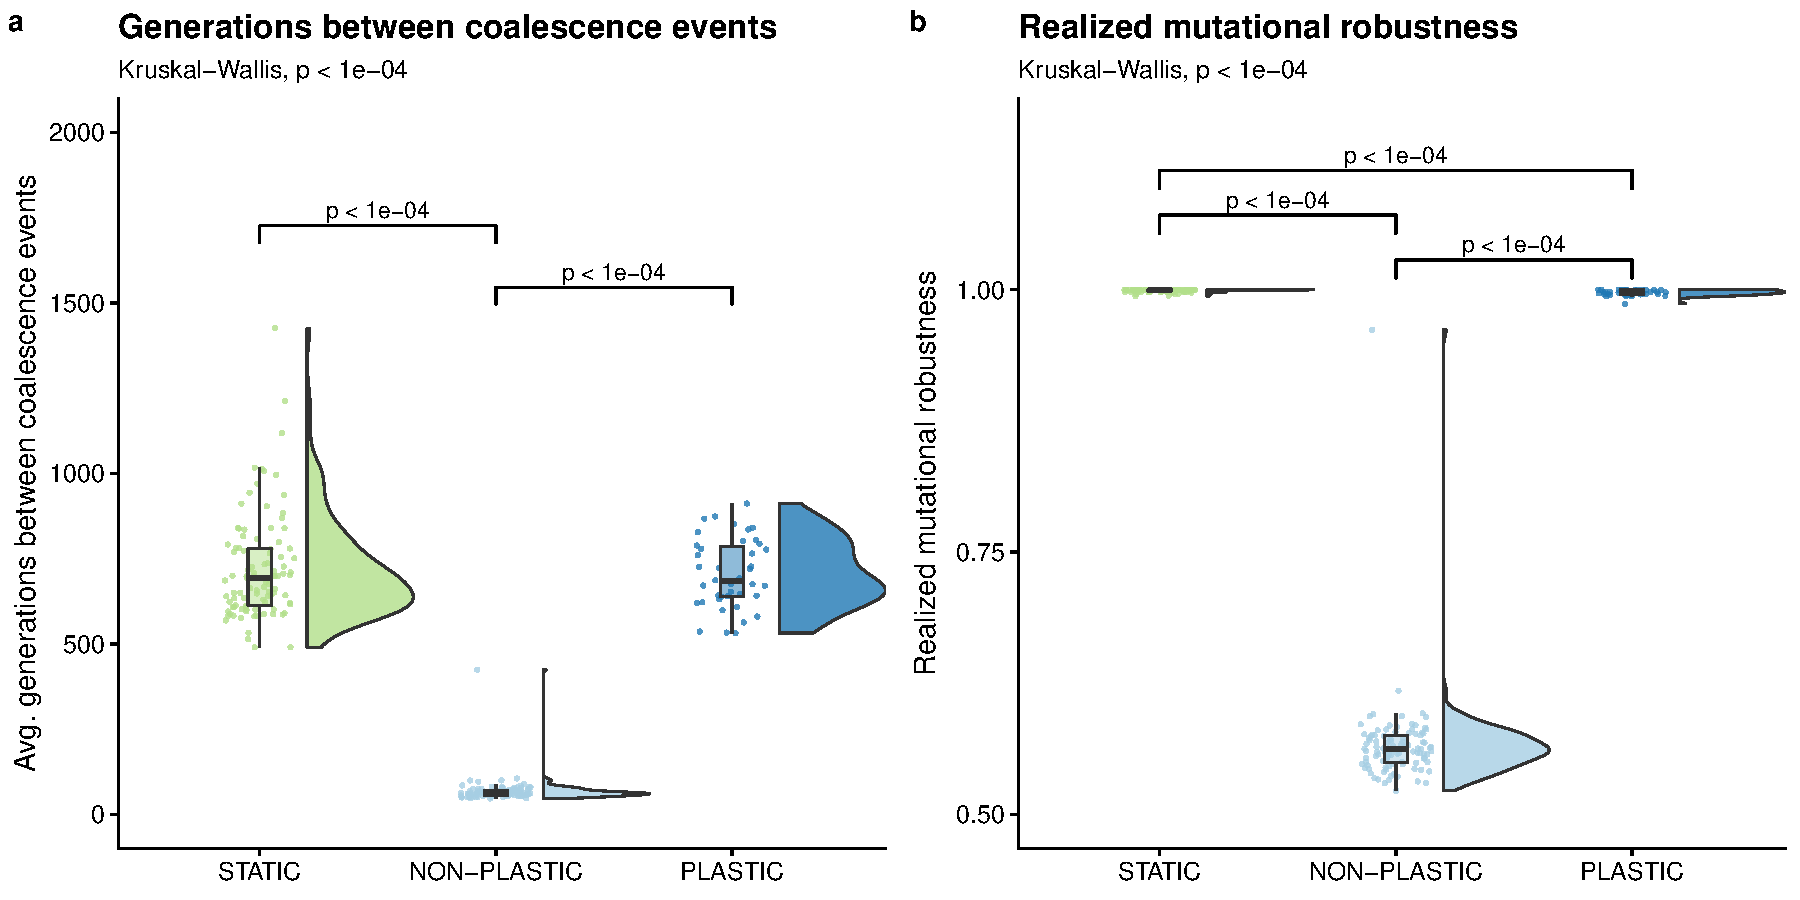
\includegraphics[width=0.66\textwidth]{02_consequences_of_plasticity/media/media-evolutionary-change-pace-panel.pdf}
  \caption{\small
  Raincloud plots of
  (a) average number of generations between coalescence events,
  and (b) realized mutational robustness (Table \ref{tab:metrics-definitions}).
  Each plot is annotated with statistically significant comparisons (Bonferroni-corrected pairwise Wilcoxon rank-sum tests).
  }
  \label{fig:evolutionary-dynamics-rate}
\end{figure}

% -- Rate of evolutionary change => findings --
On average, significantly fewer generations elapsed between coalescence events in NON-PLASTIC populations than in either PLASTIC or STATIC populations (Figure \ref{fig:evolutionary-dynamics-rate}a).
We also found that both STATIC and PLASTIC lineages exhibited higher realized mutational robustness relative to that of NON-PLASTIC lineages (Figure \ref{fig:evolutionary-dynamics-rate}b); that is, mutations observed along NON-PLASTIC lineages more often caused phenotypic changes in offspring.
Overall, our results indicate that NON-PLASTIC populations underwent more rapid (and thus a greater amount of) evolutionary change than either PLASTIC or STATIC populations.

% -- Mutational stability in static and plastic lineages --
While both STATIC and PLASTIC lineages exhibited high realized mutational robustness, we found that STATIC lineages exhibited higher realized robustness than PLASTIC lineages (Figure \ref{fig:evolutionary-dynamics-rate}b).
Overall, there were rare instances of mutations that caused a change in phenotypic profile across all PLASTIC lineages.
Of these mutations, we found that over 80\% (83 out of 102) of changes to phenotypic profiles were cryptic.
That is, the mutations affected traits that would not have been expressed in the environment that the organism was born into but would have been expressed had the environment changed.

\begin{figure}[ht!]
  \centering
  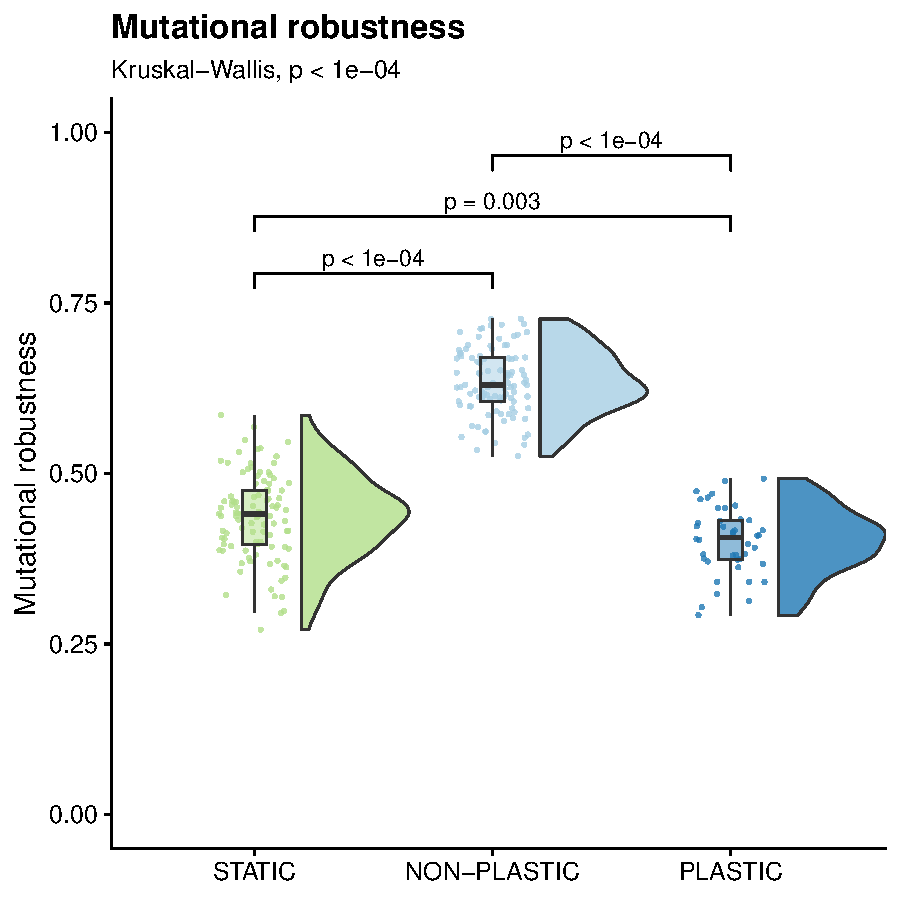
\includegraphics[width=0.33\textwidth]{02_consequences_of_plasticity/media/media-mutational-robustness.pdf}
  \caption{\small
      Raincloud plot of mutational robustness of each representative genotype (Table \ref{tab:metrics-definitions}).
      The plot is annotated with statistically significant comparisons (Bonferroni-corrected pairwise Wilcoxon rank-sum tests).
  }
  \label{fig:mutational-robustness}
\end{figure}

% -- mutational landscaping --
% Thus far, our analyses have focused on dominant lineage.
% What about mutations off the line of descent?
% Mutational stability result is NOT due to random mutations being more likely to induce phenotypic change.
% KEY: Motivation for looking at mutational neighborhoods needs to made very clear here
%   - Why not look at mutational neighborhoods for the other experiments?
Given that NON-PLASTIC lineages exhibited the lowest realized mutational robustness of our three experimental treatments, we sought to determine if this effect was driven by differences in evolved genetic architectures.
Specifically, did the NON-PLASTIC genetic architectures evolve such that mutations were more likely to result in phenotypic change?
Such a mutational bias would trade off descendant fitness in the same environment in exchange for a chance of increasing descendant fitness in alternate environments.
This strategy would be an example of diversifying bet-hedging (\textit{i.e.}, reducing expected mean fitness to lower variance in fitness) \citep{childs2010evolutionary}.
Alternatively, the lower realized mutational robustness in NON-PLASTIC lineages could be due to survivorship bias, as we measured realized mutational robustness as the fraction of mutations observed along \textit{successful} lineages that caused a phenotypic change.
That is, our measure of realized mutational robustness concentrates only on mutations that appear in the representative lineage (\textit{i.e.}, ``survivors'' of selection), ignoring mutations that did not. 
Thus, lower realized mutational robustness in NON-PLASTIC lineages could simply be due to phenotype-altering mutations being more frequently favored by selection.
%(\textit{i.e.}, the lineages of extant organisms)


We analyzed the mutational robustness of representative genotypes by calculating the fraction of single-instruction mutations that change the phenotypic profile.
We found that mutations to representative genotypes on NON-PLASTIC lineages are \textit{less} likely to result in a phenotypic change than mutations to comparable genotypes on either STATIC or PLASTIC lineages (Figure \ref{fig:mutational-robustness}).
These data provide evidence against NON-PLASTIC lineages engaging in a mutation-driven bet-hedging strategy, and instead, are consistent with the hypothesis that lower realized mutational robustness in the NON-PLASTIC treatment was due to survivorship bias.
% @AML: Maybe one more sentence elaborating on implication of survivorship bias?

% -- in general, PLASTIC and STATIC more similar than NON-PLASTIC --
In general, adaptive plasticity stabilized PLASTIC-treatment populations against environmental fluctuations, and their evolutionary dynamics more closely resembled those of populations evolving in a static environment.
We observed no significant difference in the number and frequency of coalescence events in PLASTIC and STATIC populations.
We did, however, observe small, but statistically significant, differences in each of the following metrics: elapsed generations,  mutation counts, phenotypic volatility, realized mutational robustness, and mutational robustness between PLASTIC and STATIC populations.  
We expect that these differences are a result of plastic organisms needing to simultaneously maintain both function and function-regulation machinery, resulting in more genetic components that can be broken by mutations; moreover, many of these components are under relaxed selection in periods between environmental changes.
Overall, these differences were not substantial enough to play an obvious role in any of the dynamics we analyzed, but could be examined further in the future.

\subsection{Adaptively plastic populations retain more novel functions than non-plastic populations in fluctuating environments}

%%%%%%%%%%%%%%%%%%%%%%%%%%%%%%%%%
% Results to report (2021-01-31)
% - Number of plastic replicates
% - Final dominant genotype # novel traits
%   - non-plastic < (plastic == static)
% - Final population (1% threshold):
%   - non-plastic < plastic < static
% - Final population (1% threshold) discovered:
%   - non-plastic > (plastic ~~ static)
% - Lineage functions discovered
%   - non-plastic > static ~>(nosig) plastic
% - Lineage functions discovered / step
%   - (static ~~ plastic) > non-plastic
% - Lineage functions lost
%   - non-plastic > static > plastic
% - Lineage functions lost / step
%   - non-plastic > static > plastic

% - functions discovered per generation(?)
%   - NON-PLASTIC [0.00014358046266055] ~~ STATIC [0.00015363220504867] > PLASTIC [0.000117695011124939]
% - functions lost per generation(?)
%   - NON-PLASTIC [0.0022026054610079] > STATIC [0.000161396283669756] > PLASTIC [6.25141973661864e-05]
%%%%%%%%%%%%%%%%%%%%%%%%%%%%%%%%%

\begin{figure}[h!]
  \centering
  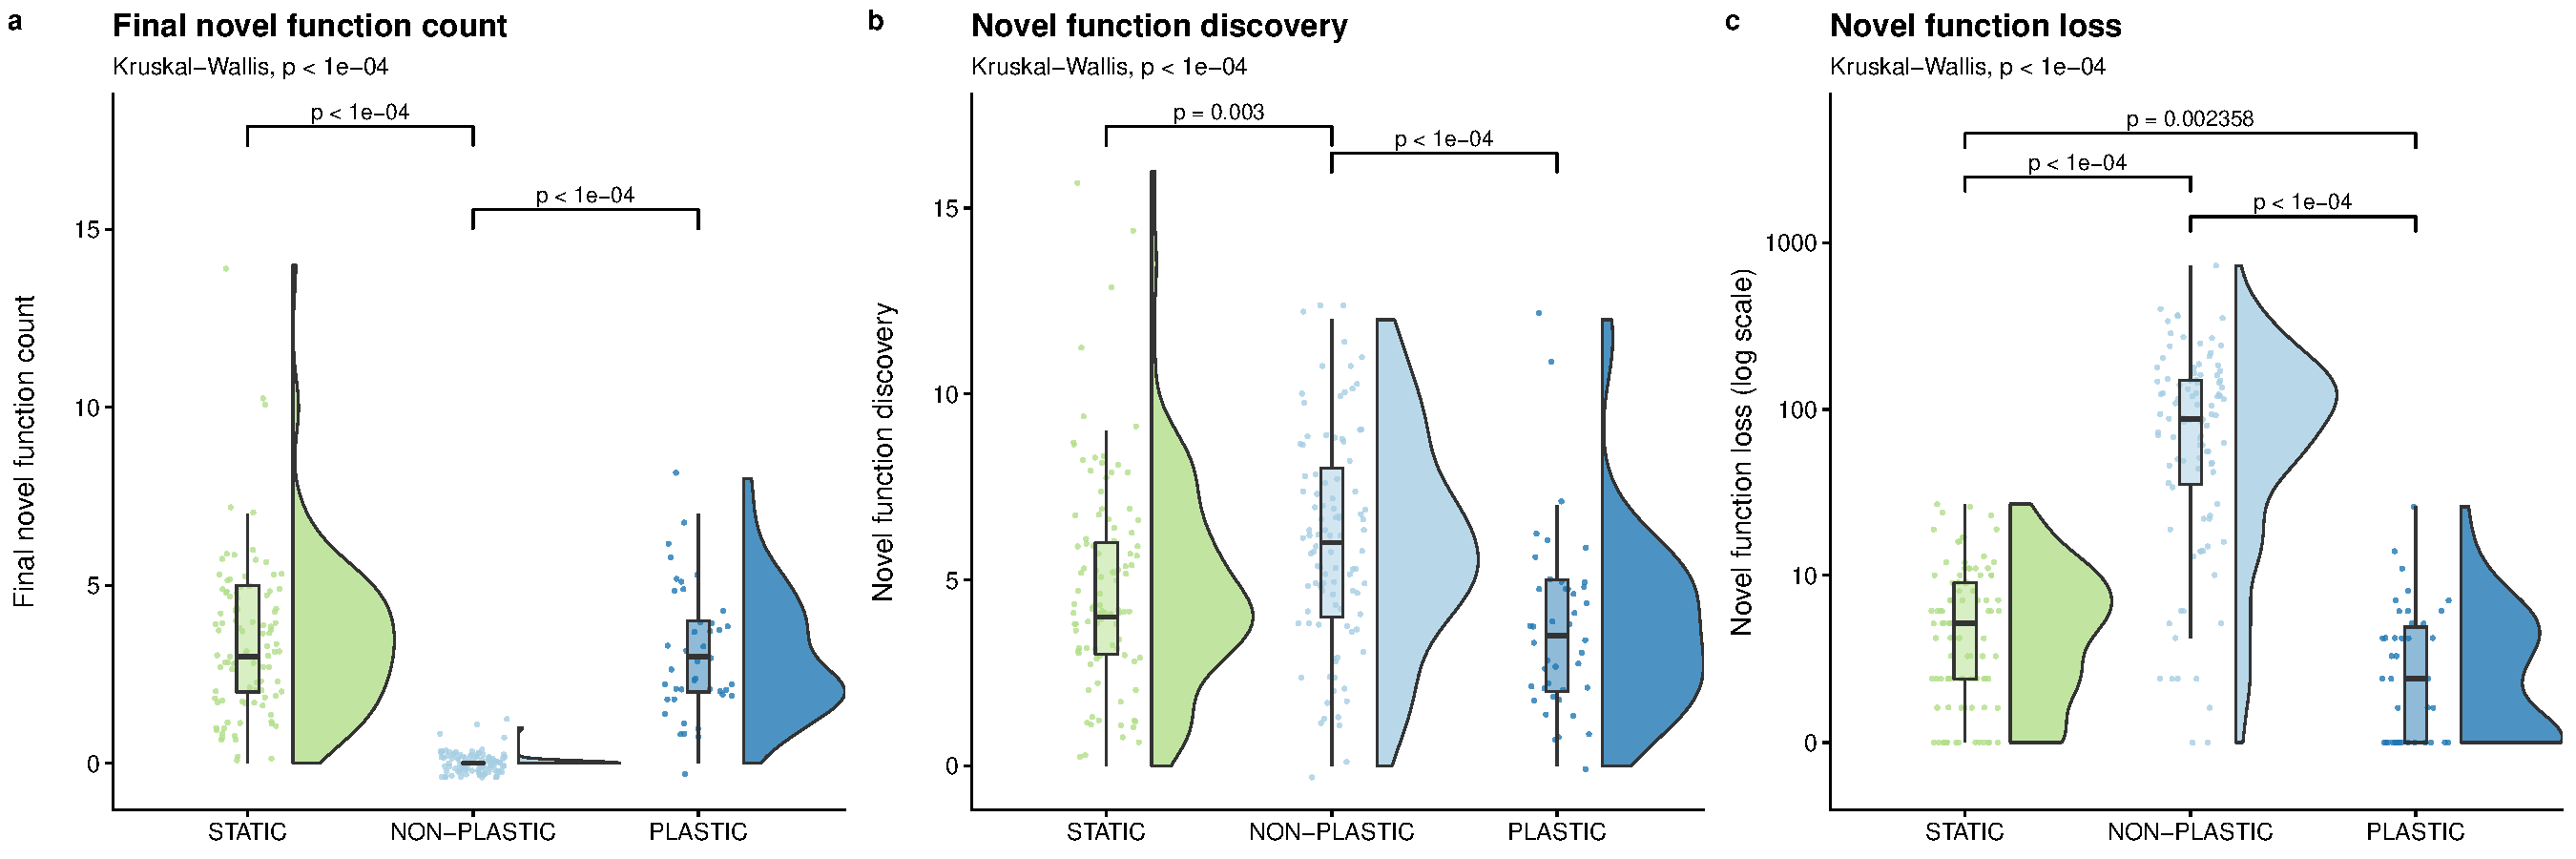
\includegraphics[width=0.9\textwidth]{02_consequences_of_plasticity/media/media-complex-traits-magnitude-panel.pdf}
  \caption{\small
  Raincloud plots of
  (a) final novel function count,
  (b) novel function discovery,
  and (c) novel function loss.
  See Table \ref{tab:metrics-definitions} for descriptions of each metric.
  Each plot is annotated with statistically significant comparisons (Bonferroni-corrected pairwise Wilcoxon rank-sum tests).
  Note that adaptive phenotypic plasticity evolved in \novelTraitsPlasticReps\ of \novelTraitsReplicates\ replicates from the PLASTIC treatment during phase one of this experiment; we used this more limited group to seed the resulting \novelTraitsPlasticReps\ phase-two PLASTIC replicates.
  }
  \label{fig:complex-traits-magnitude}
\end{figure}

% -- What did we test? --
We have so far shown that adaptive plasticity constrains the rate of evolutionary change in fluctuating environments.
However, it is unclear how this dynamic influences the evolution of novel functions.
Based on their relative rates of evolutionary change, we might expect NON-PLASTIC-treatment populations to evolve more novel functions than PLASTIC-treatment populations.
But, how much of the evolutionary change in NON-PLASTIC populations is useful for exploring novel regions of the fitness landscape versus continually rediscovering the same regions?

% - Magnitude of exploration/exploitation -
To answer this question, we quantified the number of novel functions performed by a representative organism in the final population of each replicate.
We found that both PLASTIC and STATIC populations had significantly higher final function counts than NON-PLASTIC populations at the end of the experiment (Figure~\ref{fig:complex-traits-magnitude}a).
The final novel function count in PLASTIC and STATIC lineages could be higher than that of the NON-PLASTIC lineages for several non-mutually exclusive reasons.
One possibility is that PLASTIC and STATIC lineages could be exploring a larger area of the fitness landscape when compared to NON-PLASTIC lineages.
Another possibility is that the propensity of the NON-PLASTIC lineages to maintain novel traits could be significantly lower than PLASTIC or STATIC lineages.
When we looked at the total sum of novel functions discovered by each of the PLASTIC, STATIC, and NON-PLASTIC lineages, we found that NON-PLASTIC lineages generally explored a larger area of the fitness landscape (Figure~\ref{fig:complex-traits-magnitude}b).
Although the NON-PLASTIC lineages discovered more novel functions, those lineages also exhibited significantly higher novel function loss when compared to PLASTIC and STATIC lineages (Figure~\ref{fig:complex-traits-magnitude}c).

\begin{figure}[h!]
  \centering
  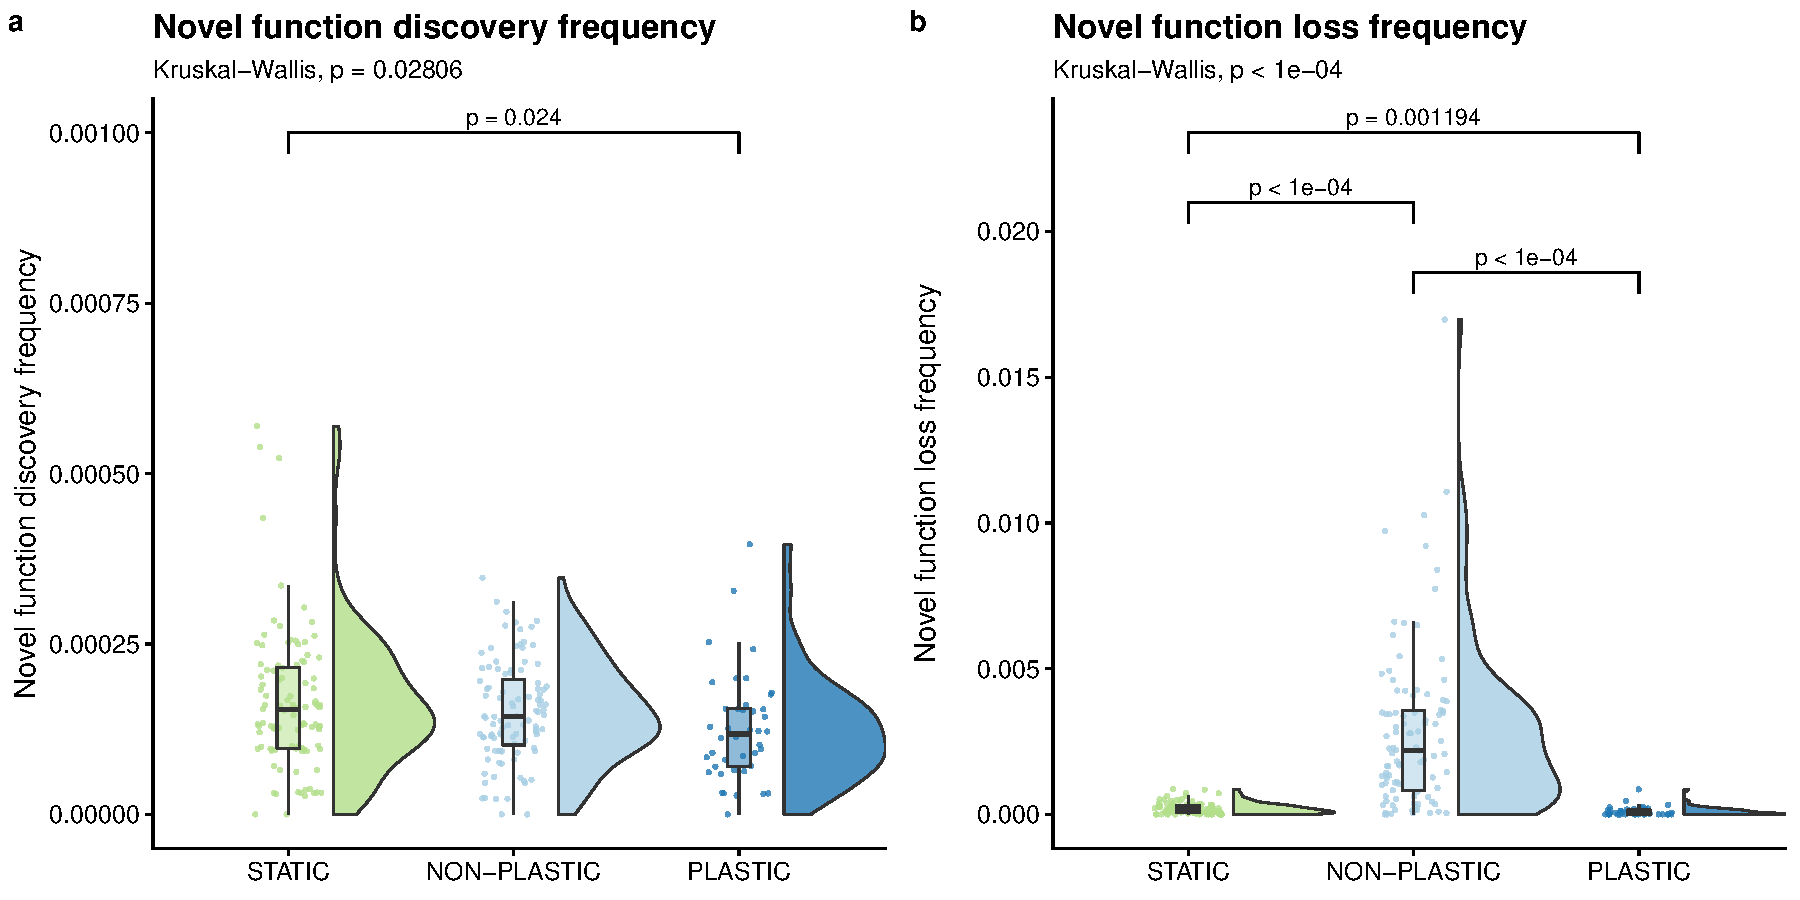
\includegraphics[width=0.66\textwidth]{02_consequences_of_plasticity/media/media-complex-traits-pace-panel.pdf}
  \caption{\small
  Raincloud plots of
  (a) novel function discovery frequency
  and (b) novel function loss frequency.
  Each plot is annotated with statistically significant comparisons (Bonferroni-corrected pairwise Wilcoxon rank-sum tests).
  }
  \label{fig:complex-traits-rate}
\end{figure}

% - Rates of exploration/exploitation -
A larger number of generations elapsed in NON-PLASTIC populations than in PLASTIC or STATIC populations during our experiment \citep{supplemental_material}.
Are NON-PLASTIC lineages discovering and losing novel functions more frequently than PLASTIC or STATIC lineages, or are our observations a result of differences in generational turnover?
To answer this question, we converted the metrics of novel function discovery and novel function loss to rates by dividing each metric by the number of elapsed generations along the associated representative lineages.
We found no significant difference in the frequency of novel function discovery between NON-PLASTIC and STATIC lineages, and we found that PLASTIC lineages had a lower frequency of novel function discovery than STATIC lineages (Figure~\ref{fig:complex-traits-rate}a).
Therefore, we cannot reject the possibility that the larger magnitude of function discovery in NON-PLASTIC lineages was driven by a larger number of elapsed generations.
NON-PLASTIC lineages had a higher frequency of function loss than either PLASTIC or STATIC lineages, and PLASTIC lineages tended to have a lower frequency of novel function loss than STATIC lineages (Figure~\ref{fig:complex-traits-rate}b).


% - Characterizing trait loss -
Next, we examined the frequency at which novel function loss along lineages co-occurred with the loss or gain of any of the six base functions.
Across all NON-PLASTIC representative lineages, over 97\% (10998 out of 11229) of instances of novel function loss co-occurred with a simultaneous change in base function profile.
In contrast, across all PLASTIC and STATIC dominant lineages, we observed that approximately 20\% (29 out of 142) and 2\% (13 out of 631), respectively, of instances of novel function loss co-occurred with a simultaneous change in base function profile.
As such, the losses of novel functions in NON-PLASTIC lineages appear to be primarily due to hitchhiking or epistatic effects where a mutation that knocks out a maladaptive base function (after the environment changes) also knocks out a beneficial novel function.

\subsection{Lineages without plasticity that evolve in fluctuating environments express more deleterious functions}

%%%%%%
% 2021-02-05 - Results
% - Number of offspring on lineage where hitchhiker instruction execution increases (i.e., instances of hitchhiking)
%   - PLASTIC ~~ STATIC < NON-PLASTIC
% - Hitchhiker instruction increases / offspring on lineage
%   - PLASTIC ~~ STATIC < NON-PLASTIC
% - What fraction of mutations that increase hitchhiker instruction execution co-occur with base trait changes?
%   - NON-PLASTIC > PLASTIC ~~ STATIC
% - What about unexpressed vs expressed trait changes in plastic populations? (plastic only)
%   - Not much hitchhiking. Did not find evidence that hitchiking occurring as cryptic variation in unexpressed phenotype.
%%%%%%

Phenotypic plasticity allows for genetic variation to accumulate in genomic regions that are unexpressed, which could lead to the fixation of deleterious instructions in PLASTIC populations.
However, in NON-PLASTIC lineages, we observe a higher rate of novel function loss, indicating that they may be more susceptible to deleterious mutations (Figure \ref{fig:complex-traits-rate}b).

Therefore, in experiment phase 2C, we tested whether adaptive phenotypic plasticity can increase the incidence of deleterious function performance.
Specifically, we added an instruction that triggered an explicitly deleterious  function and measured the number of times it was executed.
Each execution of the \code{deleterious} instruction reduces an organism's fitness by 10\%.
At the beginning of phase 2C, the \code{deleterious} instruction is not present in the population, as it was not part of the instruction set during phase one of evolution.
Accordingly, if a \code{deleterious} instruction fixes in a population, it must be the result of evolutionary dynamics during phase 2C, including cryptic variation, hitchhiking, or as a result of sign epistasis where a \code{deleterious} instruction knocks out an even more maladaptive trait.
% sign epistasis; two things that are deleterious that are less deleterious in combination than you would expect form individual effects
% sign epistasis 

\begin{figure}[ht!]
  \centering
  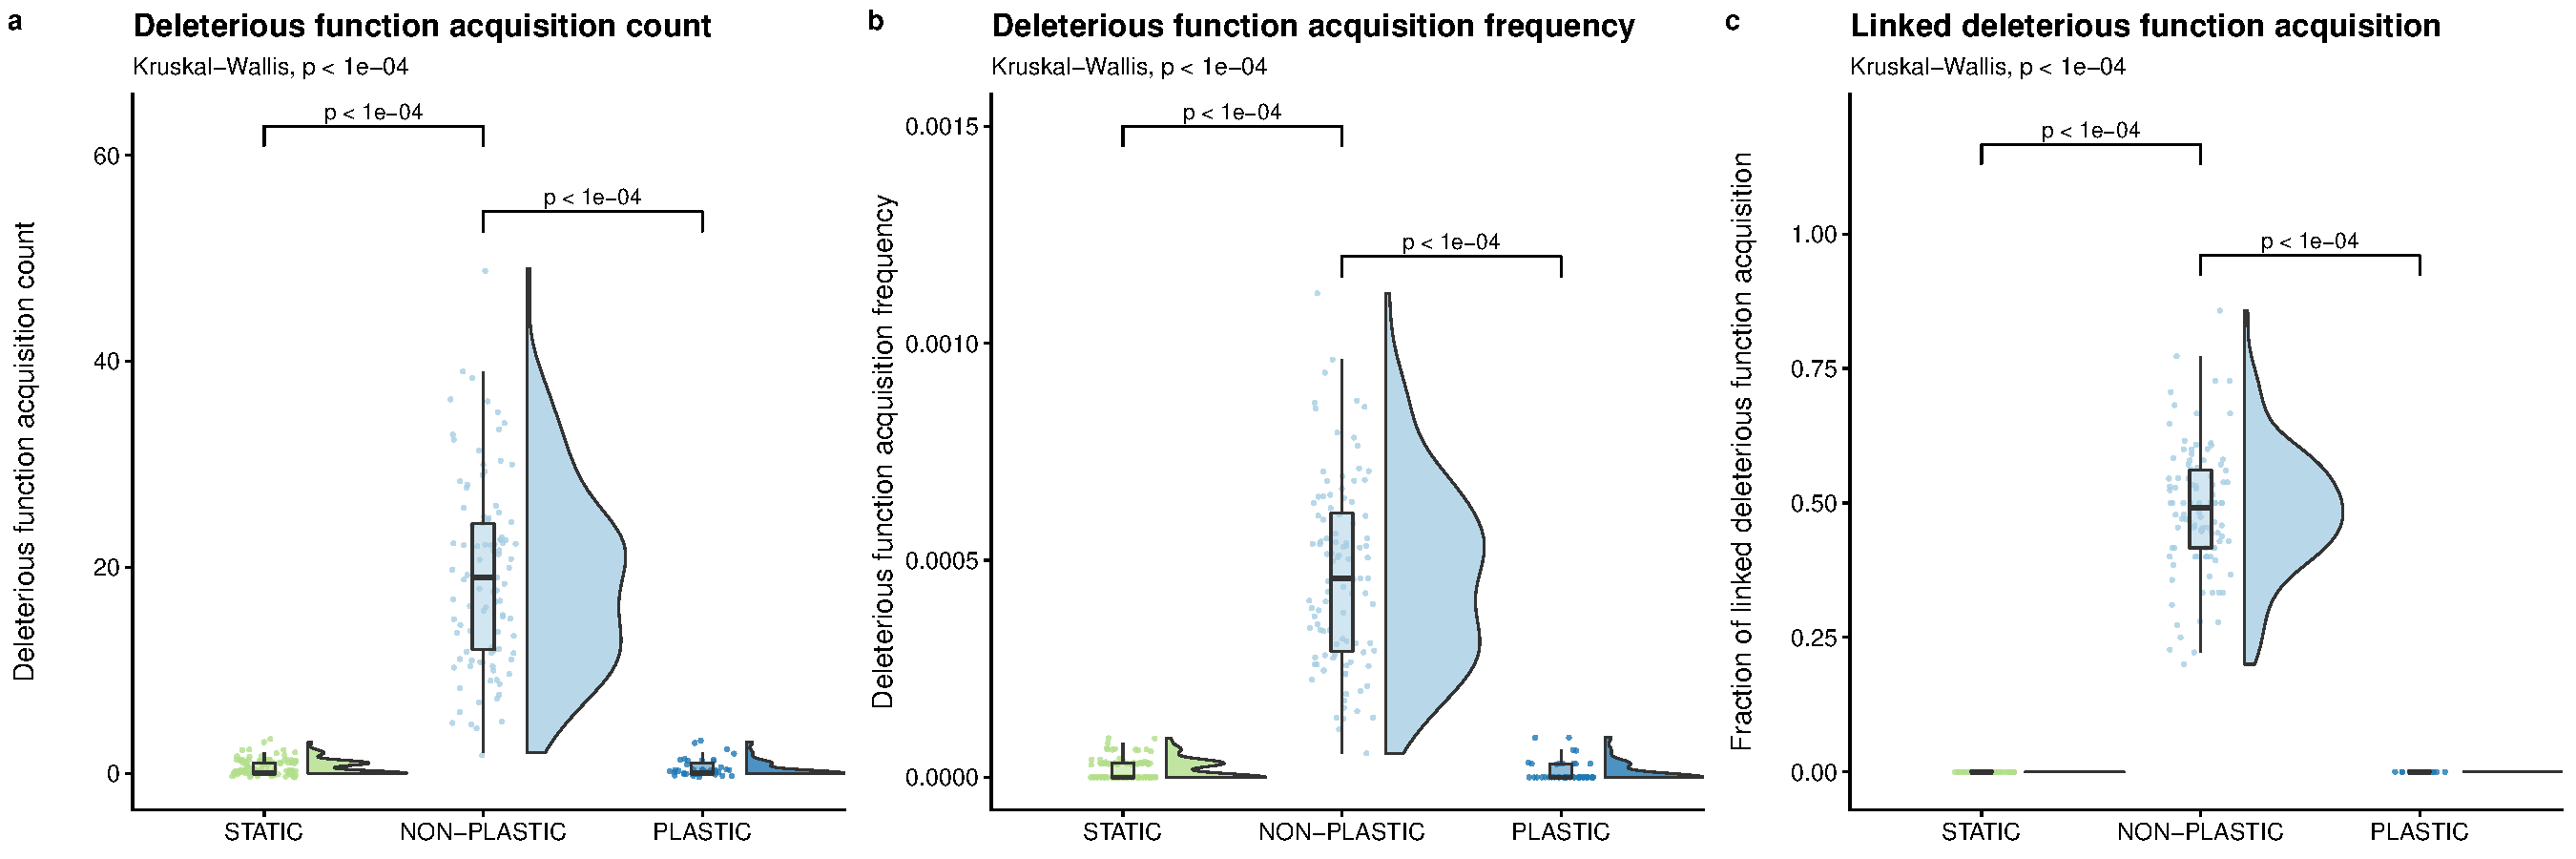
\includegraphics[width=1.0\textwidth]{02_consequences_of_plasticity/media/media-poison-accumulation-panel.pdf}
  \caption{\small
  Raincloud plots of
  (a) deleterious function acquisition,
  (b) deleterious function acquisition frequency,
  and (c) the proportion of mutations that increase deleterious function expression along a lineage that co-occur with a change in phenotypic profile.
  Each plot is annotated with statistically significant comparisons (Bonferroni-corrected pairwise Wilcoxon rank-sum tests).
  Note that adaptive phenotypic plasticity evolved in \deleteriousHitchhikingPlasticReps\ of \deleteriousHitchhikingReplicates\ replicates from the PLASTIC treatment during phase one of this experiment; we used this more limited group to seed the \deleteriousHitchhikingPlasticReps\ phase-two PLASTIC replicates.
  }
  \label{fig:deleterious-hitchhiking}
\end{figure}

% -- Instruction execution by final dominant & along lineage --
At the end of our experiment, no representative organisms from the PLASTIC or STATIC treatments performed the deleterious function under any environmental condition; however, representative organisms in 14\% of replicates of the NON-PLASTIC treatment performed the deleterious function at least once.
NON-PLASTIC lineages contained significantly more mutations that conferred the deleterious function as compared to PLASTIC or STATIC lineages (Figure \ref{fig:deleterious-hitchhiking}a), and these mutations occurred at a significantly higher frequency in NON-PLASTIC lineages (Figure \ref{fig:deleterious-hitchhiking}b).
% Additionally, we did not observe
% This result does not change when we normalize [what?] by the number of generations represented in the given lineage (Figure \ref{fig:deleterious-hitchhiking}b).

% -- When/where does hitchhiking take place? --
Next, we measured how often mutations that increased deleterious function performance co-occurred with changes to the base function profile within representative lineages.
A \code{deleterious} instruction can fix in a population by having a beneficial effect that outweighs its inherent cost (\textit{e.g.}, knocking out a punished function) or through linkage with a secondary beneficial mutation at another site within the genome.
Across all NON-PLASTIC representative lineages, we found that approximately 49\% (956 out of 1916) of mutations that increased deleterious function expression co-occurred with a change in the base function profile (Figure \ref{fig:deleterious-hitchhiking}c).
In all representative lineages from the PLASTIC treatment, only 18 mutations increased deleterious function expression, and none co-occurred with a change in base function profile (Figure \ref{fig:deleterious-hitchhiking}c).
Likewise, only 58 mutations increased deleterious function performance in all representative lineages from the STATIC treatment, and none co-occurred with a change in base function profile (Figure \ref{fig:deleterious-hitchhiking}c).
We did not find compelling evidence that the few mutations that increased deleterious function expression occurred as cryptic variation in PLASTIC lineages.

We repeated this experiment with 3\% and 30\% metabolic rate penalties associated with the deleterious function, which produced results that were consistent with those reported here \citep{supplemental_material}.


% GUIDELINES:
% This section may be divided by subheadings. Discussions should cover the key findings of the study: discuss any prior research related to the subject to place the novelty of the discovery in the appropriate context, discuss the potential shortcomings and limitations on their interpretations, discuss their integration into the current understanding of the problem and how this advances the current views, speculate on the future direction of the research, and freely postulate theories that could be tested in the future.

\section{Discussion}

In this work, we used evolving populations of digital organisms to determine how adaptive phenotypic plasticity alters subsequent evolutionary dynamics and influences evolutionary outcomes in fluctuating environments.
Specifically, we compared lineages of adaptively plastic organisms in fluctuating environments to both non-plastic organisms in those same environments and other non-plastic organisms in static environments.

\subsection{Evolutionary change}

% -- Adaptively plastic populations underwent less evolutionary change than non-plastic populations --
We found strong evidence that adaptive plasticity slows evolutionary change in fluctuating environments.
Adaptively plastic populations experienced fewer coalescence events and fewer total genetic changes relative to non-plastic populations evolving under identical environmental conditions (Figure \ref{fig:evolutionary-dynamics-magnitude}).
Whereas non-plastic populations relied on \textit{de novo} mutations to adapt to each environmental fluctuation, plastic populations leveraged sensory instructions to regulate function performance.
Indeed, in fluctuating environments, selection pressures toggle after each environmental change.
We hypothesize that in non-plastic populations such toggling would repeatedly drive the fixation of mutations that align an organism's phenotypic profile to the new conditions.
This hypothesis is supported by the increased frequency of coalescence events in these populations (Figure \ref{fig:evolutionary-dynamics-rate}a) as well as increased rates of genetic and phenotypic changes observed along the lineages of non-plastic organisms.

% - Mutational neighborhood results
Representative lineages in the non-plastic treatment experienced lower realized mutational robustness than plastic and static lineages (Figure~\ref{fig:evolutionary-dynamics-rate}b).
We reasoned that this lower realized mutational robustness was due to non-plastic populations evolving a bet-hedging strategy where mutations are more likely to modify the phenotypic profile.
However, when we switched from measuring the realized mutational robustness of representative lineages to measuring the mutational robustness of representative genotypes (\textit{i.e.}, what fraction of one-step mutants change the phenotypic profile), we observed that non-plastic genotypes exhibited the highest mutational robustness of all three treatments (Figure~\ref{fig:mutational-robustness}).
This result runs contrary to both our expectations and the results of other fluctuating environment studies in Avida~\citep{canino-koning_fluctuating_2019}.
\cite{canino-koning_fluctuating_2019} found that mutational robustness is negatively correlated with the number of function-encoding sites in the genome.
In our work, most plastic and static genotypes encode all six base functions, while most non-plastic genotypes only encode functions from one environment; this results in fewer function-encoding sites, which may increase mutational robustness in non-plastic genotypes (relative to plastic and static genotypes). %relative to genotypes from other treatments.
Regardless of the cause, this higher mutational robustness in non-plastic organisms indicates that bet-hedging is not driving the low realized mutational robustness observed in non-plastic lineages.
Thus, we expect the lower realized mutational robustness in non-plastic lineages to be driven by survivorship bias.
Because non-plastic lineages must rely on mutations to adapt to environmental changes, phenotype-altering mutations are often highly advantageous, and their selection decreases the realized mutational robustness of successful lineages.


% -- in context of previous digital evolution work --
To our knowledge, this study is the first in-depth empirical investigation into how the \textit{de novo} evolution of adaptive plasticity shifts the course of subsequent evolution in a cyclic environment.
The relative rates of evolutionary change that we observed in non-plastic populations, however, are consistent with results from previous digital evolution studies.
For example, \cite{dolson_interpreting_2020} showed that non-plastic populations that were evolved in cyclically changing environments exhibited higher phenotypic volatility and accumulated more mutations than that of populations evolved under static conditions.
Furthermore, \cite{lalejini_evolutionary_2016} visually inspected the evolutionary histories of non-plastic organisms evolved in fluctuating environments, observing that mutations along successful lineages readily switched the set of traits expressed by offspring.
%\cite{canino-koning_evolution_2016} also observed that genomes evolved in harsh cyclic environments often contained vestigial fragments of genetic material adapted to prior environments.


% -- In context of conventional evolutionary theory: evo response => f(selection, variation) --
Our results are also consistent with conventional evolutionary theory.
A trait's evolutionary response to selection depends on the strength of directional selection and on the amount of genetic variation for selection to act upon \citep{lande_measurement_1983,zimmer_evolution_2013}.
In our experiments, non-plastic populations repeatedly experienced strong directional selection to toggle which functions were expressed after each environmental change.
As such, retrospective analyses of successful lineages revealed rapid evolutionary responses (that is, high rates of genetic and phenotypic changes).
Evolved adaptive plasticity shielded populations from strong directional selection when the environment changed by eliminating the need for a rapid evolutionary response to toggle function expression.
Indeed, both theoretical and empirical studies have shown that adaptive plasticity can constrain evolutionary change by weakening directional selection on evolving populations \citep{price_role_2003,paenke_influence_2007,ghalambor_non-adaptive_2015}.

% TODO, consider: Expectations that could arise if we took into consideration lineages off the line of descent.

\subsection{The evolution and maintenance of novel functions}

% -- Exploration + Exploitation --
In fluctuating environments, non-plastic populations explored a larger area of the fitness landscape than adaptively plastic populations (Figure \ref{fig:complex-traits-magnitude}b).
However, adaptively plastic populations better exploited the fitness landscape, retaining a greater number of novel functions than non-plastic populations evolving under identical environmental conditions (Figure \ref{fig:complex-traits-magnitude}a).
In our experiment, novel functions were less important to survival than the fluctuating base functions.
In non-plastic populations, when a mutation changes a base function to better align with current environmental conditions, its benefit will often outweigh the cost of losing one or more novel functions.
Indeed, we found that along non-plastic representative lineages, 97\% of the mutations associated with novel function loss co-occurred with phenotypic changes that helped offspring adapt to current environmental conditions.

% -- Changing environments promote evolutionary change --
Previous studies have shown that transitory environmental changes can improve overall fitness landscape exploration in evolving populations of non-plastic digital organisms \citep{nahum_improved_2017}.
Similarly, changing environments have been shown to increase the rate of evolutionary adaptation in simulated network models \citep{kashtan2007varying}.
In our system, however, we found that \textit{repeated} fluctuations reduced the ability of non-plastic populations to maintain and exploit functions; that said, we did find that repeated fluctuations may improve overall function discovery by increasing generational turnover.
Consistent with our findings, \cite{canino-koning_fluctuating_2019} found that non-plastic populations of digital organisms evolving in a cyclic environment maintained fewer novel traits than populations evolving in static environments.

% -- Plastic rescue, stabilizing effect of plasticity --
Our results suggest that adaptive phenotypic plasticity can improve the potential for populations to exploit novel resources by stabilizing them against stressful environmental changes.
The stability that we observe may also lend some support to the hypothesis that phenotypic plasticity can rescue populations from extinction under changing environmental conditions \citep{chevin_adaptation_2010}.

% -- relevance to genes as followers hypothesis --.
Our data do not necessarily provide evidence for or against the genes as followers hypothesis.
The genes as followers hypothesis focuses on contexts where plastic populations experience novel or abnormally stressful environmental change.
However, in our system, environmental changes were cyclic (not novel), and no single environmental change was \textit{abnormally} stressful.
Further, the introduction of novel functions during the second phase of the experiment merely added static opportunities for fitness improvement.
This addition did not change the meaning of existing environmental cues, nor did it require those cues to be used in new ways.

\subsection{The accumulation of deleterious alleles}

% -- Overview of results --
%   - More accumulation in non-plastic
%   - no evidence for cryptic variation housing poison
%   - plastic ~~ static
We found that non-plastic lineages that evolved in a fluctuating environment exhibited both greater totals and higher rates of deleterious function acquisition than that of adaptively plastic lineages (Figure \ref{fig:deleterious-hitchhiking}).
There are several, non-mutually exclusive possibilities that could explain the fixation of explicitly deleterious instructions: random genetic drift, deleterious hitchhiking, epistatic effects, and cryptic variation (in plastic organisms).
We find it unlikely that random genetic drift explains our observations.
Each time an organism expresses a \code{deleterious} instruction, the organism incurs a 10\% penalty to their replication rate, which results in strong purifying selection against mutations that cause offspring to execute \code{deleterious} instructions.

In asexual populations without horizontal gene transfer, all co-occurring mutations are linked.
As such, deleterious mutations linked with a stronger beneficial mutation (\textit{i.e.}, a driver) can sometimes ``hitchhike'' to fixation \citep{smith_hitch-hiking_1974,van_den_bergh_experimental_2018,buskirk_hitchhiking_2017}.
Natural selection normally prevents deleterious mutations from reaching high frequencies, as such mutants are outcompeted.
However, when a beneficial mutation sweeps to fixation in a clonal population, it carries along any linked genetic material, including other beneficial, neutral, or deleterious mutations \citep{barton_genetic_2000, smith_hitch-hiking_1974}.
Therefore, deleterious genetic hitchhiking could have contributed to \code{deleterious} instruction accumulation along non-plastic lineages in changing environments.

% Antagonistic pleiotropy occurs when a mutation has beneficial effects for one trait but also causes deleterious effects on other traits~\citep{zimmer_evolution_2013}. 
Epistatic effects (\textit{i.e.}, interactions between genes) could have also contributed to \code{deleterious} instruction accumulation along non-plastic lineages. 
On their own, mutations that increase \code{deleterious} instruction execution are maladaptive; however, if such a mutation were to also knock out an even more harmful function, that mutation may have a net beneficial effect.
As such, mutations that confer increased \code{deleterious} instruction execution could directly drive a selective sweep. 

% Across our experiments, the frequency of selective sweeps in non-plastic populations provided additional opportunities for genetic hitchhiking and antagonistic pleiotropy with each environmental change.
% Indeed, 
Representative lineages from non-plastic populations in the cyclic environment exhibited higher mutation accumulation (Figure~\ref{fig:evolutionary-dynamics-magnitude}b), novel function loss (Figure~\ref{fig:complex-traits-magnitude}c), and deleterious function acquisition (Figure~\ref{fig:deleterious-hitchhiking}a) than their plastic counterparts.
In aggregate, we found that many ($\sim$49\%; 956 / 1916) mutations that increased \code{deleterious} instruction execution in offspring co-occurred with mutations that provided an even stronger benefit by adapting the offspring to an environmental change.
We expect that an even larger fraction of these deleterious mutations were linked to beneficial mutations, but our analysis only counted mutations that co-occurred in the same generation.
Our analyses did not distinguish between epistatic effects and deleterious hitchhiking; however, more fine-grained analyses of secondary effects of mutations that conferred \code{deleterious} instruction execution could be performed in future work to disentangle these two mechanisms.


% -- Elaboration on plastic result --
Theory predicts that under relaxed selection deleterious mutations should accumulate as cryptic variation in unexpressed traits \citep{lahti_relaxed_2009}.
Contrary to this expectation, we did not find evidence of \code{deleterious} instructions accumulating as cryptic variation in adaptively plastic lineages.
One possible explanation is that the period of time between environmental changes was too brief for variants carrying unexpressed \code{deleterious} instructions to drift to high frequencies before the environment changed, after which purifying selection would have removed such variants.
Indeed, we would not expect drift to fix an unexpressed trait since we tuned the frequency of environmental fluctuations to prevent valuable traits from being randomly eliminated during the off environment.
Additionally, plastic organisms in Avida usually adjust their phenotype by toggling the expression of a minimal number of key instructions, leaving little genomic space for cryptic variation to accumulate.

\subsection{Limitations and future directions}

% ------------
% Possible additional future directions:
% - Need to look at mutations off the line of descent
% - Variable length genomes
% - Relaxed selection, mutational decay
% ------------

% -- Adaptive vs non-adaptive plasticity --
Our work lays the groundwork for using digital evolution experiments to investigate the evolutionary consequences of phenotypic plasticity in a range of contexts.
However, the data presented here are limited to the evolution of \textit{adaptively} plastic populations.
Future work might explore the evolutionary consequences of maladaptive and non-adaptive phenotypic plasticity (\textit{e.g.}, \citealt{leroi_temperature_1994}), which are known to bias evolutionary outcomes~\citep{ghalambor_non-adaptive_2015}.

% -- Environmental change --
Additionally in our experiments, sensory instructions perfectly differentiated between ENV-A and ENV-B, and environmental fluctuations never exposed populations to entirely new conditions.
These parameters have been shown to influence evolutionary outcomes~\citep{li_digital_2004,boyer_adaptation_2021}, which if relaxed in the context of further digital evolution experiments, may yield additional insights.
Our experiments also focused on asexually reproducing digital organisms. 
Sexual reproduction has been shown to be advantageous in rapidly changing environments, such as the cyclic environments used in our study~\citep{misevic_experiments_2010}. 
Future work could investigate how sexual reproduction affects the evolutionary consequences of adaptive plasticity. 

% - limitation: focus on lineages -
%   - extend to complete evolutionary histories
We focused our analyses on the lineages of organisms with the most abundant genotype in the final population.
These successful lineages represented the majority of the evolutionary histories of populations at the end of our experiment, as populations did not exhibit long-term coexistence of different clades.
Our analyses, therefore, gave us an accurate picture of what fixed in the population.
We did not, however, examine the lineages of extinct clades.
Future work will extend our analyses to include extinct lineages, giving us a more complete view of evolutionary history, which may allow us to better distinguish adaptively plastic populations from populations evolving in a static environment.

% - Machinery -
As with any wet-lab experiment, our results are in the context of a particular model organism: ``Avidian'' self-replicating computer programs.
Digital organisms in Avida regulate responses to environmental cues using a combination of sensory instructions and conditional logic instructions (\code{if} statements).
The \code{if} instructions conditionally execute a single instruction depending on previous computations and the state of memory.
As such, plastic organisms in Avida typically regulate phenotypes by toggling the expression of a small number of key instructions as opposed to regulating cohorts of instructions under the control of a single regulatory sequence \citep{supplemental_material}.
This bias may limit the accumulation of hidden genetic variation in Avida genomes.
However, as there are many model biological organisms, there are many model digital organisms that have different regulatory mechanisms (\textit{e.g.}, \citealt{lalejini_evolving_2018}) that should be used to test the generality of our results.

% -- Reviewer 1 comment --
% With a population size of 3600 individuals and a genomic mutation rate of 0.25 mutations/genome/generation, potential beneficial mutations are generated quickly and selective sweeps occur quickly
% "One can imagine that a larger population with a decreased mutation rate would not see the observed phenomenon due to differences in the dynamics of selective sweeps."
% "Altering the time spent in each environment may alter this trend of selective sweeps driving deleterious mutation accumulation. "
As with most digital evolution experiments, our mutation rates were high and population sizes were small (3600 individuals) relative to experiments with microbes or conditions common in nature.
As such, beneficial mutations can be generated rapidly and selective sweeps can occur quickly.
Moreover, our analyses were limited to a single rate of environmental change and simple function reward structures, which likely influenced the rates of selective sweeps observed in our experiments. 
Future studies could address these limitations by increasing population sizes, decreasing mutation rates, investigating different function rewards and punishments, and altering the time spent in each environment. %, painting a more complete picture of the range of scenarios where our results apply.


\end{raggedbottom}

\section*{Supplemental Material}

The supplemental material for this article is hosted on GitHub and can be found online at \url{https://github.com/amlalejini/evolutionary-consequences-of-plasticity} \citep{supplemental_material}.

\section*{Data Availability Statement}

The datasets generated and analyzed for this study can be found on the Open Science Framework at \url{https://osf.io/sav2c/} \citep{osf_data}.
% \documentclass[letterpaper]{article}

% \usepackage{natbib,alifeconf,amsmath,multirow,makecell,hyperref}  %% The order is important
% \usepackage[table]{xcolor}


% *****************
%  Requirements:
% *****************
%
% - All pages sized consistently at 8.5 x 11 inches (US letter size).
% - PDF length <= 8 pages for full papers, <=2 pages for extended
%    abstracts (not including citations).
% - Abstract length <= 250 words.
% - No visible crop marks.
% - Images at no greater than 300 dpi, scaled at 100%.
% - Embedded open type fonts only.
% - All layers flattened.
% - No attachments.
% - All desired links active in the files.

% Note that the PDF file must not exceed 5 MB if it is to be indexed
% by Google Scholar. Additional information about Google Scholar
% can be found here:
% http://www.google.com/intl/en/scholar/inclusion.html.


% If your system does not generate letter format documents by default,
% you can use the following workflow:
% latex example
% bibtex example
% latex example ; latex example
% dvips -o example.ps -t letterSize example.dvi
% ps2pdf example.ps example.pdf


% For pdflatex users:
% The alifeconf style file loads the "graphicx" package, and
% this may lead some users of pdflatex to experience problems.
% These can be fixed by editing the alifeconf.sty file to specify:
% \usepackage[pdftex]{graphicx}
%   instead of
% \usepackage{graphicx}.
% The PDF output generated by pdflatex should match the required
% specifications and obviously the dvips and ps2pdf steps become
% unnecessary.


% Note:  Some laser printers have a serious problem printing TeX
% output. The use of ps type I fonts should avoid this problem.


%\title{Investigating the Evolution of Associative Learning with Analytical Replay Experiments}
%\title{Quantifying potentiation changes in the evolution of associative learning}
%\title{Historical contingency plays a substantial role in the evolution of associative learning}
% The evolution of associative learning is driven by historically contingent potentiating mutations
% The evolution of associative learning in digital organisms is driven by historically contingent potentiating mutations
%\title{Potentiating mutations facilitate the evolution of associative learning in digital organisms}
%\title{Intelligence and Historical Contingency: Potentiating mutations facilitate the evolution of associative learning in digital organisms}
%\title{Historical contingency in the evolution of intelligence: Potentiating mutations facilitate the evolution of associative learning in digital organisms}
\chapter{Potentiating mutations facilitate the evolution of associative learning in digital organisms}
%\chapter{Historical contingency in the evolution of intelligence: Potentiating mutations facilitate the evolution of associative learning in digital organisms}
\label{chap:learning_case_studies}

\noindent
Authors: Austin J. Ferguson and Charles Ofria 

\noindent This chapter is adapted from \citep{fergusonPotentiatingMutationsFacilitate2023}, which was peer-reviewed and published in the proceedings of the 2023 Conference on Artificial Life. 

In this work we use analytic replay experiments to quantify how the probability of evolving associative learning (i.e., its potentiation) changes over the course of evolved digital lineages. 
Specifically, we replay four case study lineages that successfully evolved learning. 
We find that potentiation can increase suddenly and identify ``potentiating mutations'' in each lineage that substantially increase potentiation in a single generation. 
We then dive into the mechanics of these mutations and how they interact with later mutations to confer associative learning. 

% KEY TERMS: Historical contingency, associative learning, replay experiments, potentiation, potentiating mutation
%\title{Locking in Evolution: Case Studies of Potentiating Mutations in/for Associative Learning}
%\title{Locking in Learning: Case Studies of Potentiating Mutations in the Evolution of Associative Learning}
% \author{Austin J. Ferguson$^{1,2,3,*}$, Charles Ofria$^{1,2,3}$  \\
% \mbox{}\\
%  $^1$Department of Computer Science and Engineering
%  $^2$Program in Ecology, Evolution, and Biology\\
%  $^3$BEACON Center for the Study of Evolution in Action \\
%  Michigan State University, East Lansing, MI 48824 \\
% $^*$fergu358@msu.edu} % email of corresponding author


% For several authors from the same institution use the same number to
% refer to one address.
%
% If the names do not fit well on one line use
%         Author 1, Author 2 ... \\ {\Large\bf Author n} ...\\ ...
%
% If the title and author information do not fit in the area
% allocated, place \setlength\titlebox{<new height>} after the
% \documentclass line where <new height> is 2.25in



% \begin{document}
% \maketitle

% \begin{abstract}
% % Abstract length should not exceed 250 words
% % 210/250 words used
% (250 words max, shorter preferred).
When a new evolutionary dynamic is identified, researchers often struggle to understand its long-term effects on evolutionary outcomes.
Evolutionary prediction is always challenging, as subtle nuances of dynamics can interact in unpredictable ways.
Digital evolution systems, however, provide an empirical alternative to prediction: automated replay experiments can be conducted in large numbers to measure a real distribution of outcomes from a given starting point.
Changes in distributions over time can help us understand the long-term implications of seemingly minor events during evolution.
We apply this technique to ``adaptive momentum'', a new framework that explains how phenomena like selective sweeps can temporarily weaken selection and enhance the likelihood of crossing deleterious fitness valleys.
We show that deleterious mutations along the leading edge of a selective sweep can have an outsized influence on the evolutionary fate of a population.
Indeed, we see that evolutionary potential to cross new deleterious valleys drastically increases during selective sweeps.
Moreover, each valley crossing initiates a new sweep, increasing the potential for further discoveries; this increased potential subsides only once all sweeps have concluded.
While we still have much to learn about both adaptive momentum and the role of history in evolution, this work identifies important evolutionary dynamics at play and hones our tools for further studies.

% \end{abstract}

\section{Introduction}

 % Lead in, get the reader thinking about analyzing evolutionary probabilities retrospectively
How likely is the evolution of a particular trait?
Researchers have long been interested in predicting evolutionary outcomes, but the inherent stochasticity in the process makes this goal exceptionally challenging.
In order to make more accurate predictions, we would need to better understand how and why the underlying probabilities of potential outcomes change over time.
%What if we instead turn the concept on its head? 
Looking purely retrospectively at evolution in nature, this type of analysis is not possible (at least not without a time machine).
%If we look at lineages that successfully evolved that particular trait, can we start to analyze how the likelihood of evolving the trait changed over time? 
%How did the history of that lineage factor into these likelihoods?
%Experimental evolution allows us to test hypotheses that are extremely difficult, if not impossible, to test in the natural world.
Leveraging the flexibility and controls available in experimental evolution, however, allows us to empirically test questions that were previously only hypothetical \citep{kaweckiExperimentalEvolution2012}. 
Here, we focus on Stephen Jay Gould's idea of ``replaying the tape of life'' \citep{gouldWonderfulLifeBurgess1990}.
The idea is simple: If we were to start life over again from the same initial conditions, would evolution follow the same pathway?
Alas, Gould remarked that this experiment is unfortunately impossible. 

% Introduce analytical replay experiments (and likely the rest of Zach's 2018 paper)
While it may be impossible to replay the \textit{entire} tape of life, practitioners of experimental evolution have conducted this experiment on a smaller scale. 
\cite{travisanoExperimentalTestsRoles1995}, \cite{wagenaarInfluenceChanceHistory2004}, and \citet{blountHistoricalContingencyEvolution2008} introduced and refined methods of investigating the role of historical contingency in evolving populations: parallel and analytic replay experiments.
By evolving multiple populations from the same starting organisms, researchers can identify the range and distribution of outcomes.
These populations can be evolved simultaneously from a given starting point (parallel replays), however many microbial and digital populations allow us to preserve a ``fossil record'', opening up another possibility.
Analytic replay experiments systematically revive historical populations to re-evolve them from multiple time points, allowing researchers to identify alternative possibilities after the fact \citep{blountContingencyDeterminismEvolution2018}.
For a more thorough review of the story behind analytic replay experiments and an overview of several papers that have used them, see Chapter \ref{chap:intro}.
%When one strain of \textit{E. coli} in Dr. Richard Lenski's long-term evolution experiment \citep{lenskiLongtermExperimentalEvolution1991} unexpectedly evolved the ability to digest citrate,  
%\citet{blountHistoricalContingencyEvolution2008} used analytic replay techniques on previously frozen samples (spaced across the lineage) to identify the potentiation of this unlikely evolutionary outcome.
%By routinely storing organisms throughout an experiment, researchers can create a ``fossil record'' of the population leading up to the evolution of a focal trait or behavior. 
%Unlike normal fossils, these historical populations (likely either microbiological or digital) can be revived.
%Because of this, researchers can seed new populations using the various time points before the focal behavior evolved and let these new populations evolve independently of the original lineage. 
%Observing whether the same behavior evolves in these new ``replay'' populations will then shed light on what led up to the original change in behavior -- whether the genetic background ``potentiated'' the change or if it was due to happenstance.
%In their replay experiments, restarts from earlier time points never re-evovled citrate utilization, but the probability (potentiation) to evolve this trait jumped substantially shortly before the actual evolution occurred. 
%They were able to identify that early replays never re-evovled citrate utilization, but an increase in potentiation resulted in replicates 
%In their replay experiments, restarts from earlier time points never re-evolved citrate utilization, but successful re-evolution of the behavior in restarts from later time points indicated that the population had become potentiated. %experienced potentiating mutations the probability (potentiation) to evolve this trait jumped substantially shortly before the actual evolution occurred. 
%In later work, \citet{blountGenomicAnalysisKey2012} used genetic sequencing and manipulation to identify the specific potentiating mutations associated with this increased probability.

%Analytic replay experiments provide a powerful new tool for understanding the role of history in evolution. 
%In addition to studying the evolution of \textit{E. coli} citrate metabolization, analytic replay experiments have also been used to study the evolution of novel receptor usage of Phage $\lambda$ into \textit{E. coli} \citep{meyerRepeatabilityContingencyEvolution2012}, and colistin resistance in \textit{Pseudomonas aeruginosa} \citep{jochumsenEvolutionAntimicrobialPeptide2016a}.
%For a review of these experiments and other uses of analytic replay experiments, see \citep{blountContingencyDeterminismEvolution2018}.

In this work we use digital evolution, specifically the evolution of self-replicating computer programs in the Avida Digital Evolution Platform \citep{ofriaAvidaSoftwarePlatform2004a}, which has previously been used to conduct replay experiments.
%Replay experiments have also been used in digital systems. 
\citet{yedidHistoricalContingentFactors2008} employed this technique to investigate the re-evolution of traits following an extinction episode, while  
\citet{covertiiiExperimentsRoleDeleterious2013} used analytic replay experiments to study the importance of individual deleterious mutations in the evolution of complex traits.
% Potentially cite Dave Bryson's dissertation: https://d.lib.msu.edu/etd/693/datastream/OBJ/View/

% Using associative learning as our example complex behavior
% Why choose associative learning
We selected associative learning as a complex behavior to study potentiation.
Associative learning is a non-trivial capability exhibited by most complex organisms.
In digital evolution systems like Avida, it serves as a rare yet evolvable trait \citep{pontesEvolutionaryOriginAssociative2020}.
For an Avida organism to exhibit associative learning, it must be capable of sensing its environment, taking action, and storing information in memory. 
% What has been done to study the evolution of associative learning before?
The evolution of associative learning has been studied via experimental evolution in both digital \citep{pontesEvolutionaryOriginAssociative2020, mcgregorEvolutionAssociativeLearning2012} and natural systems \citep{dunlapExperimentalEvolutionPrepared2014a, meryExperimentalEvolutionLearning2002}, yet many questions remain about how it evolves.
% List some ways its been studied
% However, there are still countless questions left unanswered...
While more complex forms of learning are found in nature, associative learning remains an important building block for most others and insights about how it arises may be informative for understanding the broader evolution of intelligence, especially within digital contexts.

% What we did
In this work, we begin to analyze how the likelihood of evolving a complex trait changes along a successful lineage.
Using analytic replay experiments, we identified individual mutations that cause drastic increases in the potentiation of associative learning. 
We then analyzed those mutations and their mutational neighborhoods to begin characterizing how a mutation is potentiating.  
%It is through this lens of replay experiments that we investigated the evolution of associative learning. 
%We extracted lineages that successfully evolved associative learning and then founded replay populations from various points along those lineages. 
%Initially, only a small fraction of replicates evolved associative learning when starting from the ancestral organism.
%As we founded replays along successful lineages, we could observe the changes in the fraction of successful replicates, providing evidence as to which steps in the lineages were the most beneficial for evolving associative learning. 
While these replay experiments are informative and useful for exploring counterfactual evolutionary possibilities, they are also computationally intensive.  
As such, %this work is an initial exploration of the power of this technique where 
we start by focusing on a set of case-study lineages to develop an initial framework for understanding how potentiation can occur.

% What we found
Analyzing four successful lineages, we find that potentiation can increase suddenly, even due to a single mutation.
Since these lineages were selected because they successfully evolved associative learning, potentiation generally increases in each, though some decreases do occur.
Potentiating mutations vary in initial effect, making them challenging to detect.
Retrospective analysis allows us to identify them, however, and begin hypothesizing about the dynamics that allow these mutations to potentiate associative learning.
This work demonstrates using analytic replay experiments for quantifying potentiation along a lineage and establishes baselines and techniques for future studies. 


\section{Methods}
Here we describe the digital evolution system and experiment setup used to conduct this work.

% Evolution platform: Avida in MABE2
\subsection{The Avida Digital Evolution Platform}
\label{sub-evo-software}

%%%% Shorten this paragraph -- Avida was covered in the previous chapter
This work uses the Avida Digital Evolution Platform \citep{ofriaAvidaSoftwarePlatform2004a}, which was described in Chapter \ref{chap:consequences_of_plasticity}.
Here we use an early build of version 5.0 of Avida, currently under development as part of the Modular Agent Based Evolver 2 (MABE2) framework (\href{https://github.com/mercere99/MABE2}{https://github.com/mercere99/MABE2}).
%In Avida, populations of self-replicating computer programs perform tasks to compete for CPU cycles, creating an evolution testbed that can support a wide array of experimental controls. 
Avida has previously been used to study both associative learning \citep{pontesEvolutionaryOriginAssociative2020, grabowskiEarlyEvolutionMemory2010a} and historical contingency via replay experiments \citep{yedidHistoricalContingentFactors2008, covertiiiExperimentsRoleDeleterious2013}.
Fundamentally, Avida is designed to have tools necessary to conduct work at the scale required for analytic replay experiments. 
%provides the tools necessary for conducting analytic replay experiments, while its digital nature makes the scale of this work feasible. %while its digital nature keeps experiment times manageable.
%While Avida is more complex, and thus slower, than other digital evolution models, we argue that this is appropriate for initial measurements of potentiation dynamics.
%Future work can isolate which of these dynamics are explained with simpler systems and which require more complicated interactions.

% % General intro to what we used -> Avida overview and why we used it
% This work uses an early build of version 5.0 of the Avida Digital Evolution Platform \citep{ofriaAvidaSoftwarePlatform2004a}, currently under development as part of the Modular Agent Based Evolver 2 (MABE2) framework (\href{https://github.com/mercere99/MABE2}{https://github.com/mercere99/MABE2}).
% In Avida, populations of self-replicating computer programs perform tasks to compete for CPU cycles, creating an evolution testbed that can support a wide array of experimental controls. 
% Avida has been used for numerous studies on the evolution of complexity \citep{lenski_evolutionary_2003, zamanCoevolutionDrivesEmergence2014}, associative learning \citep{pontesEvolutionaryOriginAssociative2020, grabowskiEarlyEvolutionMemory2010a}, and historical contingency via replay experiments \citep{yedidHistoricalContingentFactors2008, covertiiiExperimentsRoleDeleterious2013}.
% Fundamentally, Avida is designed to have tools necessary to conduct work at the scale required for replay experiments. %provides the tools necessary for conducting analytic replay experiments, while its digital nature makes the scale of this work feasible. %while its digital nature keeps experiment times manageable.
% While Avida is more complex, and thus slower, than other digital evolution models, we argue that this is appropriate for initial measurements of potentiation dynamics.
% Future work can isolate which of these dynamics are explained with simpler systems and which require more complicated interactions.



% What is Avida? (currently more "what are organisms in Avida?")
Avida genomes consist of assembly-like instructions that transfer data between registers, make basic comparisons, perform mathematical operations, \textit{etc}.
We use an extended instruction set that includes extra flow control and environment-specific instructions \citep{fergusonFergusonAJReplayingEvolution2023}.
%The full set of 45 instructions is available in the supplement [CITE].

% Basic process of Avida
We used Avida populations on a 60x60 toroidal grid, resulting in a population cap of 3,600 organisms.
%When reproducing, an offspring is created (possibly with mutations) and 
Offspring are placed in a grid cell next to their parent, overwriting any existing organism in that cell; the parent organism is also reset. % (but not mutated). 
During reproduction, point mutations occur in offspring at a rate of 0.0075 per instruction, while single-instruction insertion and deletion mutations occur at a rate of 0.05 per reproduction.
%We do not directly decide which organisms reproduce; 
Organisms reproduce by %executing a certain number of instructions and then 
executing the \texttt{Repro} instruction.
To prevent organisms from immediately replicating, % instead of attempting the associative learning task, 
organisms must execute 1,500 instructions before the \texttt{Repro} instruction can be activated.  
%Our influence on selection takes the form of rewards and punishments in the environment.
%Organisms that maintain a positive reward/punishment balance are able to execute more instructions, on average, and thus are more likely to successfully reproduce.


% MABE info?

\subsubsection{Associative learning}
\label{subsub-environment}
% Brief overview of the environment
%Since selection pressures in Avida come from the rewards and punishments in the environment, we must decide how that environment functions, which behaviors are rewarded, and which behaviors are punished.%, and how large these rewards and punishments are.
%For this work, 
%We created an Avida environment to test the evolution of associative learning, heavily inspired by the Avida path following environment % used in previous Avida experiments 
%\citep{pontesEvolutionaryOriginAssociative2020}. %, grabowskiEarlyEvolutionMemory2010a}.
To test the evolution of associative learning, we created a simplified version of the Avida path following environment \citep{pontesEvolutionaryOriginAssociative2020}. %, further discretizing the movements along the path.
%As in the path following environment, organisms are tasked with choosing the right action given a particular nutrient cue.
%The difference is that organism evaluation no longer occurs on a two-dimensional grid. 
%At any point, 
Instead of navigating 2D space, an organism exists in one of four states: \textit{forward}, \textit{left}, \textit{right}, or the error state, \textit{backward}.
%At any point, an organism is guaranteed to be in one of of four states: \textit{forward}, \textit{left}, \textit{right}, or \textit{backward}. 
%Each state is named for the action an organism must take to obtain an associated nutrient. % and requires the organism to execute a different instruction (with the same name as the state).%, and a nutrient cue is associated with each state. 
%By removing the dependence on a two-dimensional grid, this new environment is faster to execute and allows for randomly-generated states with no fear of paths crossing over themselves. 
%
% Details as to how the organism receives information and what it is expected to do with it
Organisms are given a \texttt{Sense} instruction, which will give them the nutrient cue of their current state. 
Using this nutrient cue, organisms need to execute the appropriate instruction (one per state) to progress along the path.
The \textit{forward} and \textit{backward} states have fixed cues (0 and -1, respectively), while, at birth, each organism is assigned random cue values for \textit{left} and \textit{right} in the range of [1, $10^{6}$]. %that persist for the organism's lifetime.
Organisms can genetically encode \textit{forward} and \textit{backward}, but must learn \textit{left} or \textit{right} in their lifetime to perfectly solve the task.
Each path begins with one of four preset starting state sequences, chosen randomly for each organism at birth, followed by additional random states. % if the organism navigated through the entire preset path. 
The four preset paths are the ``one-fixed turn'' paths from \citep{pontesEvolutionaryOriginAssociative2020}, where organisms are guaranteed to encounter a \textit{left} state before a \textit{right}.

If the organism is not in an error state and executes the appropriate instruction, they are rewarded and move to the next state. 
If an organism executes the wrong instruction (e.g., the \texttt{Left} instruction in the \textit{right} state), it is penalized and placed in the error state. 
%While in the error state, the organism will be penalized for executing the other three state-associated instructions, but upon executing the \texttt{Backward} instruction it will be placed in the previous state and allowed to try again. 
While in the error state, the organism must execute the \texttt{Backward} instruction to return to the previous state and be allowed to try again; it will be penalized for any other action. 
%This means that ``resetting'' after a bad movement is much easier than in the original path following environment. 
A cooldown is applied, however, such that executing the \texttt{Backward} instruction causes the organism to wait for the equivalent of 10 additional instruction executions.
%This cooldown allows for a much simpler mechanism of self-resetting while not significantly altering the dynamics of different strategies.
Organisms are scored based on the number of valid states they successfully traversed minus the number of incorrect moves made, with a maximum score of 300. 
Fitness is calculated as $1.25^{score}$, so each additional correct movement grants a 25\% boost in fitness regardless of the total number of correct movements.


% % Why is this associative learning
% Of the four states, \textit{forward} and \textit{backward} have set nutrient cues. 
% For every organism, \textit{forward} has a cue of 0 and \textit{backward} has a cue of -1. 
% The other two states have random cues. 
% When an organism is born, its \textit{left} and \textit{right} cues are randomized to integers in $[1,10^{6}]$.
% These cues are set for the organism's lifetime.
% Therefore, while \textit{forward} and \textit{backward} decisions can be genetically encoded, \textit{left} and \textit{right} require memory to associate the random cues to their appropriate instructions. 

% What behaviors can crop up, and how do we identify them?
In this environment, optimal behavior requires associative learning in the form of imprinting. 
Since the paths are guaranteed to have a \textit{left} state before a \textit{right} state, the optimal behavior is to find and store the first positive cue value as the \textit{left} cue.
Combined with genetically-encoded \textit{forward} and \textit{backward} logic, storing and using the \textit{left} cue is enough for organisms to identify the \textit{right} cue through a process of elimination. %indefinitely pass through states without making any errors. 
%This is easier than the trial and error approach that would be needed if there were no guarantees about the starting cue, but it still requires organisms to associate at least one random cue with a state.
Other possible behaviors involve error correction (assuming all turns are one direction, then correcting when wrong), bet-hedged learning (assuming more about the paths, e.g., that there are no instances of two lefts in a row), and various mixed strategies. 

% Classification of replicates
%We then classified the dominant genotype of each replicate. 
%To sample how the genotype handles variation in the environment, we ran each genotype in 100 trials. 
%This guarantees the genotype will be tested in each of the four path starts and with a variety of random cue values. 
To categorize the behavior of a genotype, we evaluate it in 100 trials to ensure we observe how it performs in all four environments with different random cues.
We then classify each of the 100 trials.
Trials are classified as learning if the organism correctly handles greater than 90\% of the states they were in, error correction if they always successfully navigated one turn state but not the other, and ``low activity'' if they failed to successfully navigate at least 25 states.
%Trials were classified as potentially learning if they correctly handled greater than 90\% of the states they were in.
%Trials that consistently made errors in either \textit{left} or \textit{right} yet never made errors in the opposite state were classified as error correction. 
%This typically takes the form of always executing one instruction (e.g., \texttt{Left}) when in an uncertain state, and then backing up and correcting if that was the wrong instruction. 
%Finally, trials with less than 25 correct states were classified as too small to identify.
%A full breakdown of trial classification is available in the supplement [CITE]. 
%We then used the trial classifications to classify the genotype. 
To be categorized as learning or error correction, \textit{all} 100 trials of that genotype must be of that class. 
If one or more trials were low activity, the genotype was categorized as ``bet-hedged learning'' or ``bet-hedged error correction''.
If a genotype displayed at least one learning trial and at least one error correction trial, they were classified as ``mixed bet hedging''.
Finally, all remaining genotypes were categorized as ``low activity''.
%If all trials were classified as learning, the genotype was classified as learning. 
%Similarly, error correction genotypes require that all trials are classified as error correction. 
%If some trials are classified as learning and the rest are classified as too small to identify, the genotype is classified as bet-hedged learning, and the same goes for error correction and bet-hedged error correction. 
%If some trials were classified as learning and others were classified as error-correction, we classify the genotype as mixed bet-hedging. 
%Finally, if none of the other categories fit the genotype, we classify the whole genotype as too small to classify. 
This categorization system was used across all three phases of this work.

% What did we actually do?
\subsection{Experiment framework}

\begin{figure}[h!]
\begin{center}
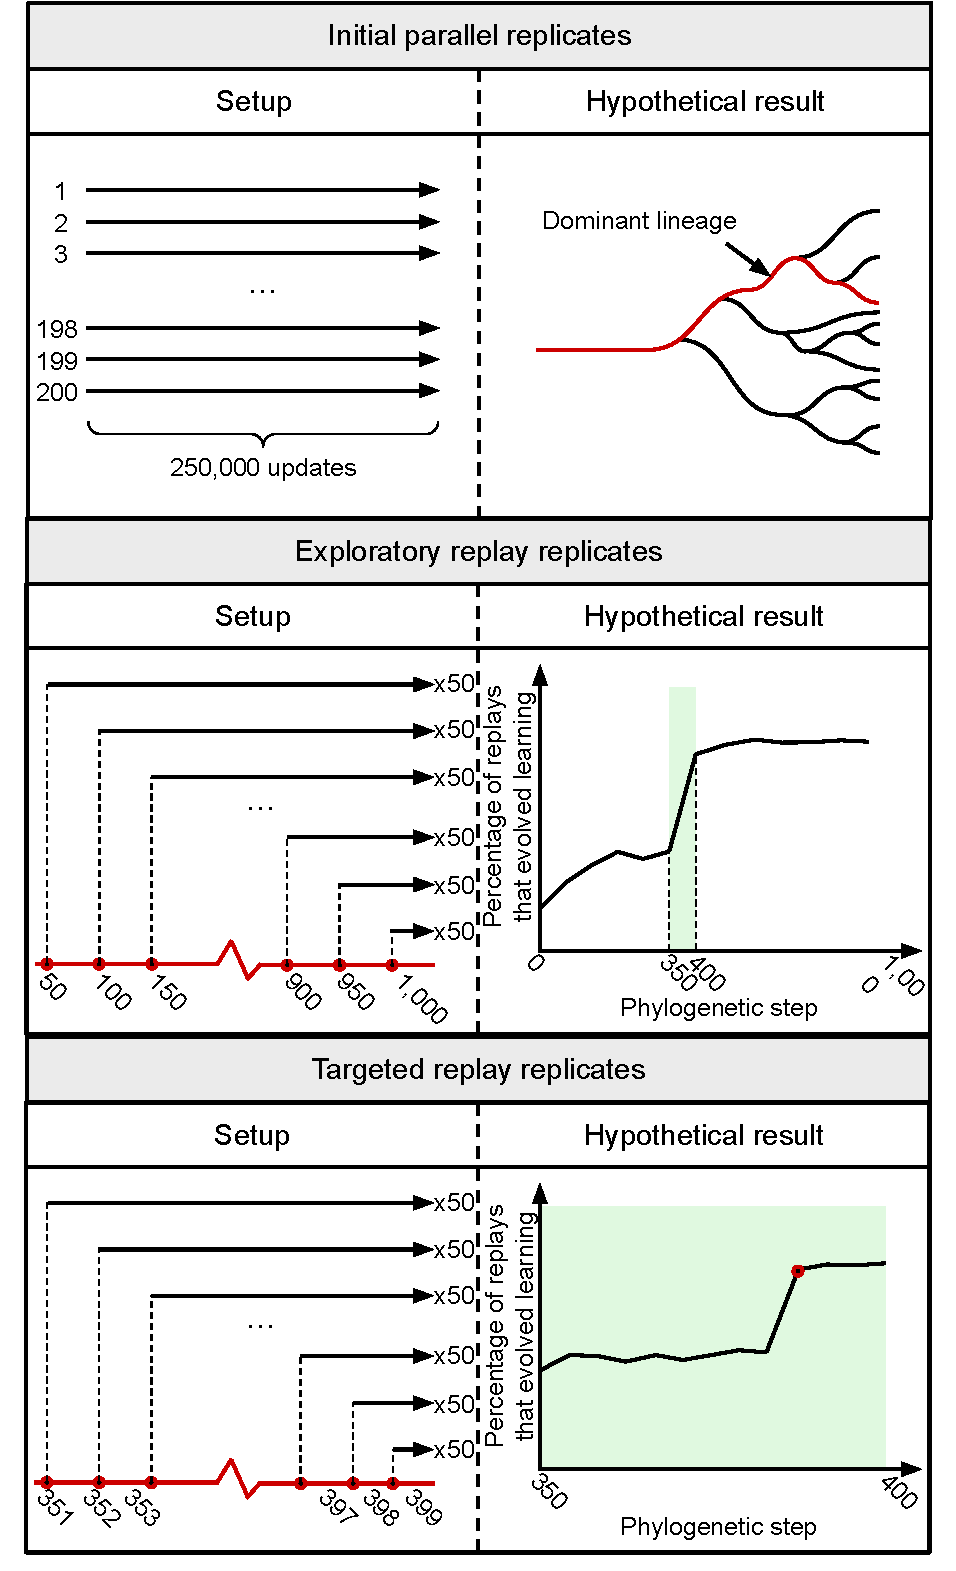
\includegraphics[width=0.65\textwidth]{03_learning_case_studies/media/conceptual_figure.pdf}
\caption{
    Illustration of the experimental design and hypothetical results.
    The top panes show the 200 initial parallel replicates seeded with the ancestral genotype and evolved for 250,000 updates.
    We extracted the lineage of the most abundant genotype in the evolved population (the dominant lineage), shown in red. 
    %When these replicates finish, we can classify each replicate and extract the dominant lineage (in red) from the phylogeny.
    Next, we conducted exploratory replays (middle panes) by launching replay replicates at regular intervals along focal lineages. 
    These exploratory replays give a coarse-grained view of how potentiation changed over a lineage. 
    We identified the window with the largest potentiation gain, shown as the shaded region.
    Finally, we ran targeted replay replicates for every step in this potentiation window. 
    %Phase 2 takes each dominant lineage from Phase 1 and launches replay experiments every 50 steps along the lineage. 
    %An example potentiation graph is shown, where a substantial increase in potentiation occurs between steps 350 and 400. 
    %We then seed \textit{additional} replay replicates for Phase 3, one for each step in the window identified in Phase 2.
    These fine-grained replay replicates show mutations that resulted in large potentiation increases (shown here with a red dot). 
}
\label{fig-conceptual}
\end{center}
\end{figure}

% Introduce three-phase design and give a brief overview of each part
To identify mutations that substantially increased the likelihood that learning evolved, we split the work into three phases (see Figure \ref{fig-conceptual} for an overview).
%
First, we seeded 200 initial parallel replicates in the associative learning environment with a default ancestor only capable of reproduction. 
Each replicate was given 250,000 updates, where one update is the time it takes for all organisms to execute 30 instructions, on average. 
% These replicates evolved for 250,000 updates, where one update is the
% and evolved them for 250,000 updates.
%For each of the 200 replicates, 
We identified the most abundant genotype in each final population to represent the replicate and classified its behavior. 
%By tracking the phylogeny in each replicate, 
We then extracted the ``dominant lineage'', stretching from the ancestor to the representative genotype. 
%(i.e., the \textit{dominant genotype} of that replicate), classified its behavior, and extracted its lineage from the ancestor. 
Each step in the lineage corresponds to a change in genotype between parent and offspring, with clonal offspring occupying the same step as their parent.
While a step is often a single mutation, it is possible that one step is composed of multiple co-occurring mutations.

To begin analyzing changes in potentiation, we ran exploratory replays replicates on four lineages capable of learning.
%Due to the computational cost of these replay experiments, we performed replays on only four learning replicates.
For each, we seeded independent replicates for every $50^{th}$ step in the lineage, up to step 1,000.
All replay replicates evolved in the same associative learning environment, and replays were given the same number of updates as had %equal to the number of updates that 
occurred after that genotype first appeared (e.g., replays for a genotype that appeared at update 150,000 would be evolved for the remaining 100,000 updates). 
Potentiation was measured as the portion of replay replicates that evolved learning. % divided by the number of replay replicates that finished. 
Because replays were seeded with a single organism, some replay populations went extinct before ever reproducing and thus were not factored in (the minimum number of finished replay replicates from a given lineage step was 38, while three case study lineages had a minimum of 48). 

While the exploratory replays provide an overview of how potentiation changed, we dug deeper by running targeted replays to further explore windows of increasing potentiation.
Specifically, we found the 50- or 100-step ``potentiation window'' that sees the largest increase in potentiation in the exploratory results, and seeded additional replays for every step in that range.
These targeted replays were conducted identically to the exploratory replays, only they did not skip steps.
Though computationally expensive, these replays illuminated the impact every genotypic change had on potentiation. 
Running 50 replay replicates per step still results in considerable noise, but we were able to identify mutations that clearly and substantially increased potentiation using these targeted replays.

We hand-analyzed algorithms in all potentiating mutations, here defined as single lineage steps that result in a potentiation increase of 25 percentage points or more.
%These potentiating mutations and other steps around them in the lineages were hand-analyzed to understand the underlying algorithm encoded in each genotype and how changes to that algorithm may have potentiated the lineage. 
Further, we assessed genotype fitness in context of their lineage to identify if potentiation mutations were beneficial, deleterious, or neutral. 
Finally, %mutation analyses were conducted to 
we characterized the local fitness landscape of each genotype (one and two mutations out), measuring the presence and fitness of nearby genotypes capable of learning. 
%All two-step mutations were analyzed for each potentiating step and the step before it, to investigate whether the potentiating step increased the presence of learning in the local landscape, increased the benefit of learning, etc. 

% We then took four lineages that exhibited learning and performed exploratory replays.
% These exploratory replays took the learning lineages and conducted a ``coarse-grained'' sampling of the lineage via analytical replay experiments. 
% We ran replay replicates for every 50 steps along the lineage, out to step 1,000. 
% This provided a window into how the likelihood of evolving learning changed over time.%, and importantly, identified any periods of substantial increases in that likelihood. 
% Finally, in we isolated these period(s) of drastic increases in likelihood and ran additional targeted replay replicates in that window (one for each step along the lineage). 
% This would then show us the impact of individual steps along the lineage, potentially highlighting single steps with massive changes in potentiation. 

% % What did our replay experiments look like?
% %\subsubsection{Analytical replay experiments}
% %After identifying the replicates that evolved learning, we can then begin to analyze their evolutionary history. 
% %We tracked phylogenetic data on all extant organisms and their ancestors, so we can trace a line of descent from the final dominant genotype to the original ancestor. 
% %After identifying the replicates that evolved learning, we then started analytical replay experiments.
% %For each learning replicate, we seeded \textit{additional} evolutionary runs along the dominant genotype's lineage. 
% %Lineages are based on genotypes, so each ``step'' corresponds to a reproduction event where one or more new mutations were introduced in the new offspring. 
% %Starting at step 50, we seeded 50 replay experiments at every $50^{\text{th}}$ step up through step 1,000. 

% %Replay replicates evolved to match the 250,000 updates of the initial replicates.
% %Replays starting from early points in the lineage thus saw more new updates than replays from points farther along the lineage. 
% %As an example, if a replay starts from step 200 and the genotype was first seen at update 100,000, we would run the replicates for step 200 for 150,000 updates. 
% %These evenly-spaced replay replicates were than manually inspected for any large jumps in potentiation. 
% %If evidence of large jumps was detected, we then seeded fine-grained replay replicates for every step between the two multiples of 50.

% % \subsubsection{Initial parallel replicates}

% % % General info, 200 reps for 250k updates starting with a default ancestor
% % We stared by founding 200 parallel replicates (see top panels of Figure \ref{fig-conceptual}). 
% % Each replicate started with one organism: the ancestor organism, which consists of 99 no-operation instructions and 1 \texttt{Repro} instruction. 
% % This organism only reproduces itself, it does not interact with the environment and thus cannot receive any rewards or punishment. 
% % Each replicate was given 250,000 updates, where one update is the time it takes for all organisms to execute 30 instructions, on average. 
% % All replicates ran in the same associative learning environment.

% % % Phylogeny tracking and isolating the final dominant genotype + lineage 
% % % CITE Emily? 
% % We tracked pruned genotypic phylogenies for these initial replicates. 
% % Digital evolution has the advantage of perfectly tracking all reproduction events and storing parent-child relationships. 
% % To reduce the storage overhead, we pruned the phylogenies to only track the extant population and any ancestors of those organisms. 
% % In the end, this gave us the lineage from the ancestral organism to any genotype in the extant population at the end of the 250,000 updates. 
% % As a representative of the final extant population, we extracted the most abundant extant genotype (i.e., the dominant genotype of that replicate) and isolated its lineage.



% \subsubsection{Exploratory replay replicates}

% After the initial parallel replicates concluded, we had a set of replicates that had evolved and maintained associative learning at the end of 250,000 updates. 
% Since we know learning evolved along each of these lineages, we are interested in how the \textit{potentiation} for learning changed along the lineages (i.e., at what points along the lineage was lineage more likely to appear than not, and where did the largest jumps in potentiation occur?).
% To investigate these changes in potentiation, we took a subset of these replicates and conducted a batch of coarse-grained replay experiments to look for large gains in potentiation while conserving computational resources.
% For a given lineage, we seeded 50 replay populations at every $50^{th}$ step along the lineage (see the middle panes of Figure \ref{fig-conceptual}.
% Regardless of the length of the lineage, we stopped at step 1,000, only continuing beyond that point if the potentiation had not approached 100\%.

% To measure potentiation at a point along the lineage, we ran the 50 replay replicates and then calculated the percentage of those replicates that evolved learning (e.g., if 30 replays out of 50 evolved learning, that point would have a potentiation of 60\%). 
% These exploratory replay replicates gave us a summary of how potentiation changed over the course of the lineage. 
% More specifically, we could look for windows containing large potentiation increases. 
% If single mutations conferred large jumps in potentiation, we would expect them to occur in windows of substantial potentiation gain.
% Since all lineages started from the same ancestor, the results from the initial parallel replicates were used for step 0 of every lineage to save computational power.

% \subsubsection{Targeted replay replicates}

% Once the exploratory replays were conducted, we had a summary of how the potentiation changed over the course of the lineage. 
% We used this exploratory replays to identify periods of drastic potentiation gain. 
% The exploratory replays occurred at every 50 steps along the lineage, so we identified the 50-step window that resulted in the greatest increase in potentiation (and for the first two lineages we took a 100-step window as to maximize our chances of finding mutations that confer large jumps in potentiation. 

% Once the target window was identified, we repeated the process of running replay experiments. 
% This time we seeded replays from every step along the lineage inside the target window. 
% While computationally expensive, this illuminates the impact every change in genotype had on potentiation. 
% While 50 replay replicates per lineage step still results in considerable variation, we were able to identify mutations that clearly and substantially increased potentiation using these targeted replays. 

% Once a potentiating step was identified, we analyzed various aspects of the genotype and the evolutionary characteristics surrounding it. 
% These potentiating steps and other steps around them in the lineages were hand-analyzed to understand the underlying algorithm encoded in each genotype and how changes to that algorithm may have potentiated the lineage. 
% Further, the genotypes were assessed in context of the lineage to identify if these potentiation events were beneficial, deleterious, or neutral in terms of fitness. 
% Finally, mutation analyses were conducted to characterize the local fitness landscape and its relationship to learning. 
% All two-step mutations were analyzed for each potentiating step and the step before it, to investigate whether the potentiating step increased the presence of learning in the local landscape, increased the benefit of learning, etc. 

% % How did we conduct our mutational analysis?
% %\subsubsection{Mutational landscape analysis}

% Not sure if we'll have real statistics, but we'll definitely have data to upload
\subsection{Data and software availability}

Both the data and the software used to conduct this work are available in the supplemental material \citep{fergusonFergusonAJReplayingEvolution2023}.
Analyses were conducted in the R statistical computing language \citep{r_core_team_r_v4} using the \textit{dplyr} package to summarize data \citep{wickhamDplyrGrammarData2022}.
Data was visualized using the \textit{ggplot2} and \textit{cowplot} packages \citep{R-ggplot2, R-cowplot}.

\section{Results}

Here we discuss the generation and analysis of the initial replicate runs, followed by the more detailed results from each of the four case study lineages.

\begin{figure}[!h]
\begin{center}
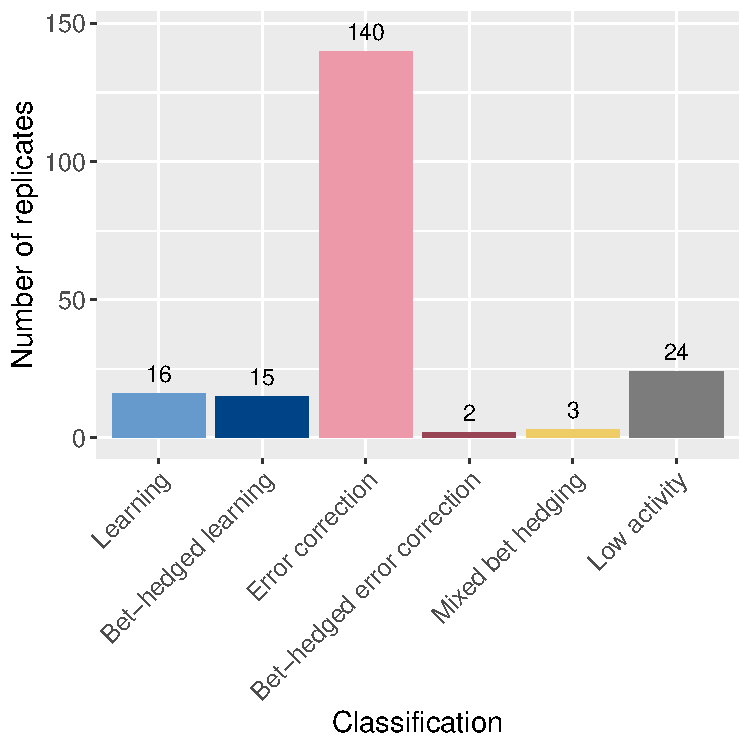
\includegraphics[width=0.65\textwidth]{03_learning_case_studies/media/final_dom_classification.pdf}
\caption{Behavior classification of the final dominant genotypes from the 200 initial parallel replicates.}
\label{fig-final-dom-classification}
\end{center}
\end{figure}

% \begin{figure}[t]
% \begin{center}
% 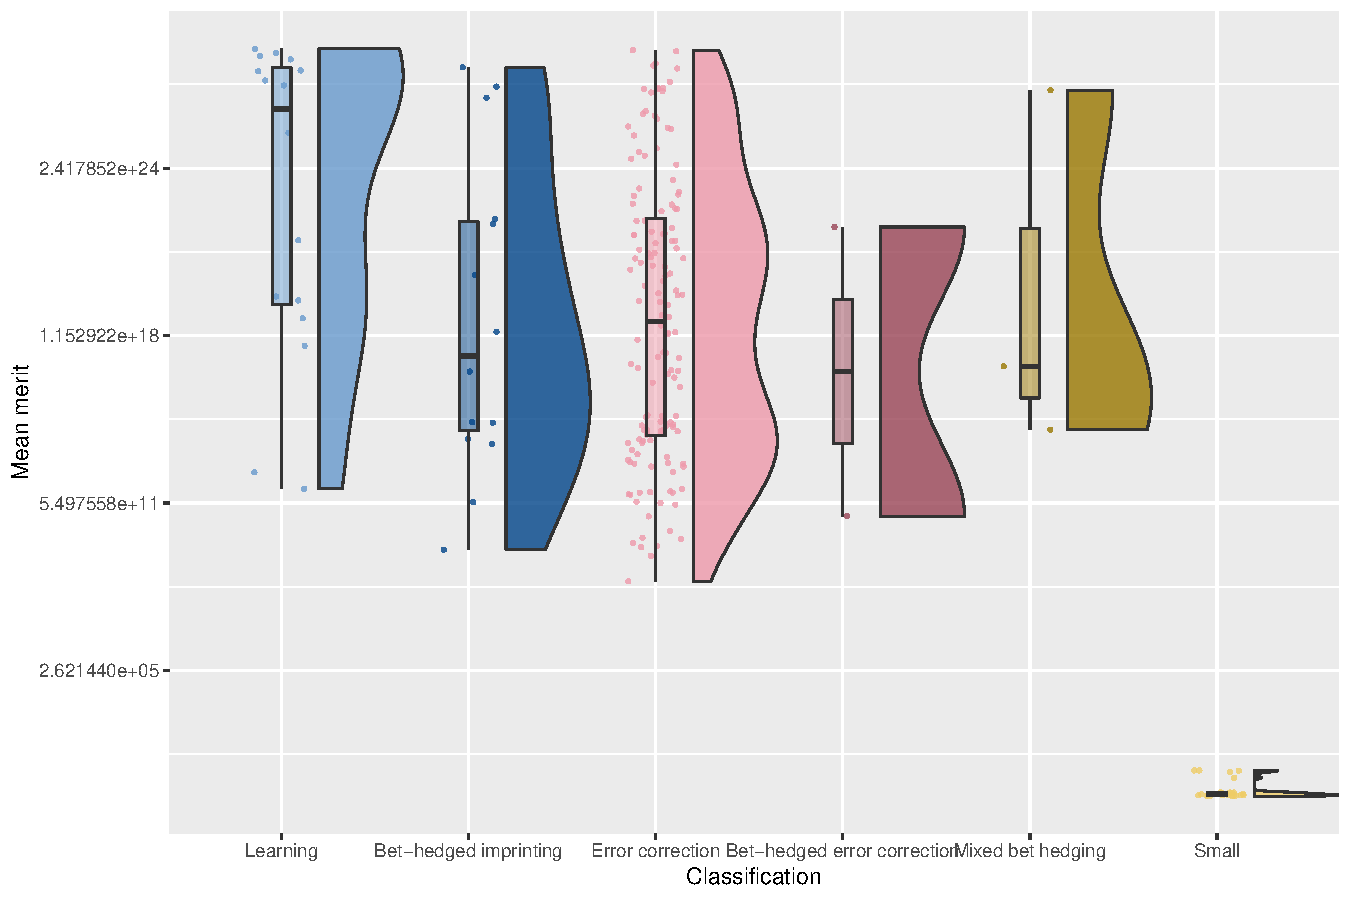
\includegraphics[width=0.45\textwidth]{media/raincloud_rep_merit.pdf}
% \caption{TODO}
% \label{fig-final-dom-rep-merit}
% \end{center}
% \end{figure}

\vspace*{-10mm}

\subsection{Evolution of learning in the initial replicates}
In the first phase of this study, we evolved 200 independent replicates for 250,000 updates (about 3600 generations) in the associative learning domain, each starting with a default ancestor. % capable only of self-replication.
%This setup allowed populations to experience approximately 3600 generations; 
The distribution of evolved behaviors is shown in Figure \ref{fig-final-dom-classification}.
Only 16 of 200 replicates exhibited associative learning.
An additional 15 replicates evolved forms of bet-hedged learning, with two of those replicates gaining and then losing associative learning along their lineage.
The majority of replicates relied on some form of error correction, either as a sole strategy (140), a bet-hedged variant (2), or as a fallback due to limited learning (3). 
%Both bet-hedged error correction replicates have a subset of environments that caused them to fall into cycles of repeatedly choosing the wrong action.%choosing the wrong action, backing up, and then choosing the same wrong action. 
%This prevented them from gaining any additional fitness. 
%Of the three mixed bet-hedging replicates, one exhibited learning in one environment and error correction in the other three
%The other two replicates exhibited the same behavior in all environments: a pseudo-learning strategy that failed on certain sequences of cues and fell back on error correction too often to hit the 90\% accuracy required to be classified as learning.
Finally, 24 replicates failed to navigate enough states to categorize them, leading us to label them as ``low activity''. 

We analyzed all 16 replicates that evolved and maintained learning, identifying the length of their lineages from onset of evolution until learning stabilized, no longer showing further improvement.
Given the substantial computational power required for each time point studied, we performed replay experiments only on the shortest three such lineages (lineages A-C), plus the shortest lineage that exhibited error correction at some point in its evolutionary history (lineage D).
%Of the 16 replicates that evolved and maintained learning, we performed replay experiments on four of them.
%The first three replicates were selected for having the shortest number of steps along a lineage before fitness stopped increasing. 
%The fourth was selected for the same reason, but was selected from among the four replicates that contained error correction in their lineages. 
%These replicates were selected to save computational resources.
%The number of updates experienced by a replay replicate was calculated as the number of updates between the genotype's first appearance in the population and the 250,000 update limit for the initial replicates. 
%Thus longer lineages A) have the potential to require more exploratory replays before saturating to $>90$\% potentiation and B) typically require more updates per replay for early steps in the lineage. 
Selecting these particular replicates to replay has the potential to bias the results, as discussed below.

% \begin{table}[!t]
% \centering
%     {\rowcolors{2}{white}{lightgray!20}
%     \begin{tabular}{ |c|c|c|c|c| }
%         \hline
% %        \makecell{Lineage} & \makecell{Initial \\ seed} & \makecell{Potentiating \\ mutation depth} & \makecell{Potentiation \\ increase} & \makecell{Fitness \\ effect} &  \makecell{Steps before \\ learning} & \makecell{Percentage of \\ updates persisted} \\
%         % \makecell{Lineage} & \makecell{Initial \\ seed} & \makecell{Potentiating \\ mutation depth} & \makecell{Potentiation \\ increase} & \makecell{Fitness \\ effect} &  \makecell{Steps before \\ learning} & \makecell{Potentiating \\ mutation persistence} \\
%         % \hline
%         % A & 86 & 484 & 58pp & Neutral & 53 & 89\% \\ 
%         % B & 4 & 104 & 36pp & Beneficial & 91 & 100\% \\ %1096 (all) \\ 
%         % C & 15 & 279 & 64pp & Deleterious & 26 & 100\% \\ %1978 (all) \\ 
%         % D & 6 & 548 & 50pp & Neutral & 8 & 100\% \\ %589 (all) \\ 
%         \makecell{Lineage} & \makecell{ mutation \\ depth} & \makecell{Potent. \\ increase} & \makecell{Fitness \\ effect} &  \makecell{Steps to \\ learning} \\
%         \hline
%         A & 484 & 58pp & Neutral & 53 \\ 
%         B & 104 & 36pp & $+$ & 91 \\ %1096 (all) \\ 
%         C & 279 & 64pp & $-$ & 26 \\ %1978 (all) \\ 
%         D & 548 & 50pp & Neutral & 8 \\ %589 (all) \\ 

%         \hline
%     \end{tabular}
%     \caption{
%     Summary of targeted replay traits.
%     }
%     \label{tab:replay-summary}
%     }
% \end{table}



\subsection{Case studies of individual lineages}

\begin{figure*}[!th]
    \begin{center}
    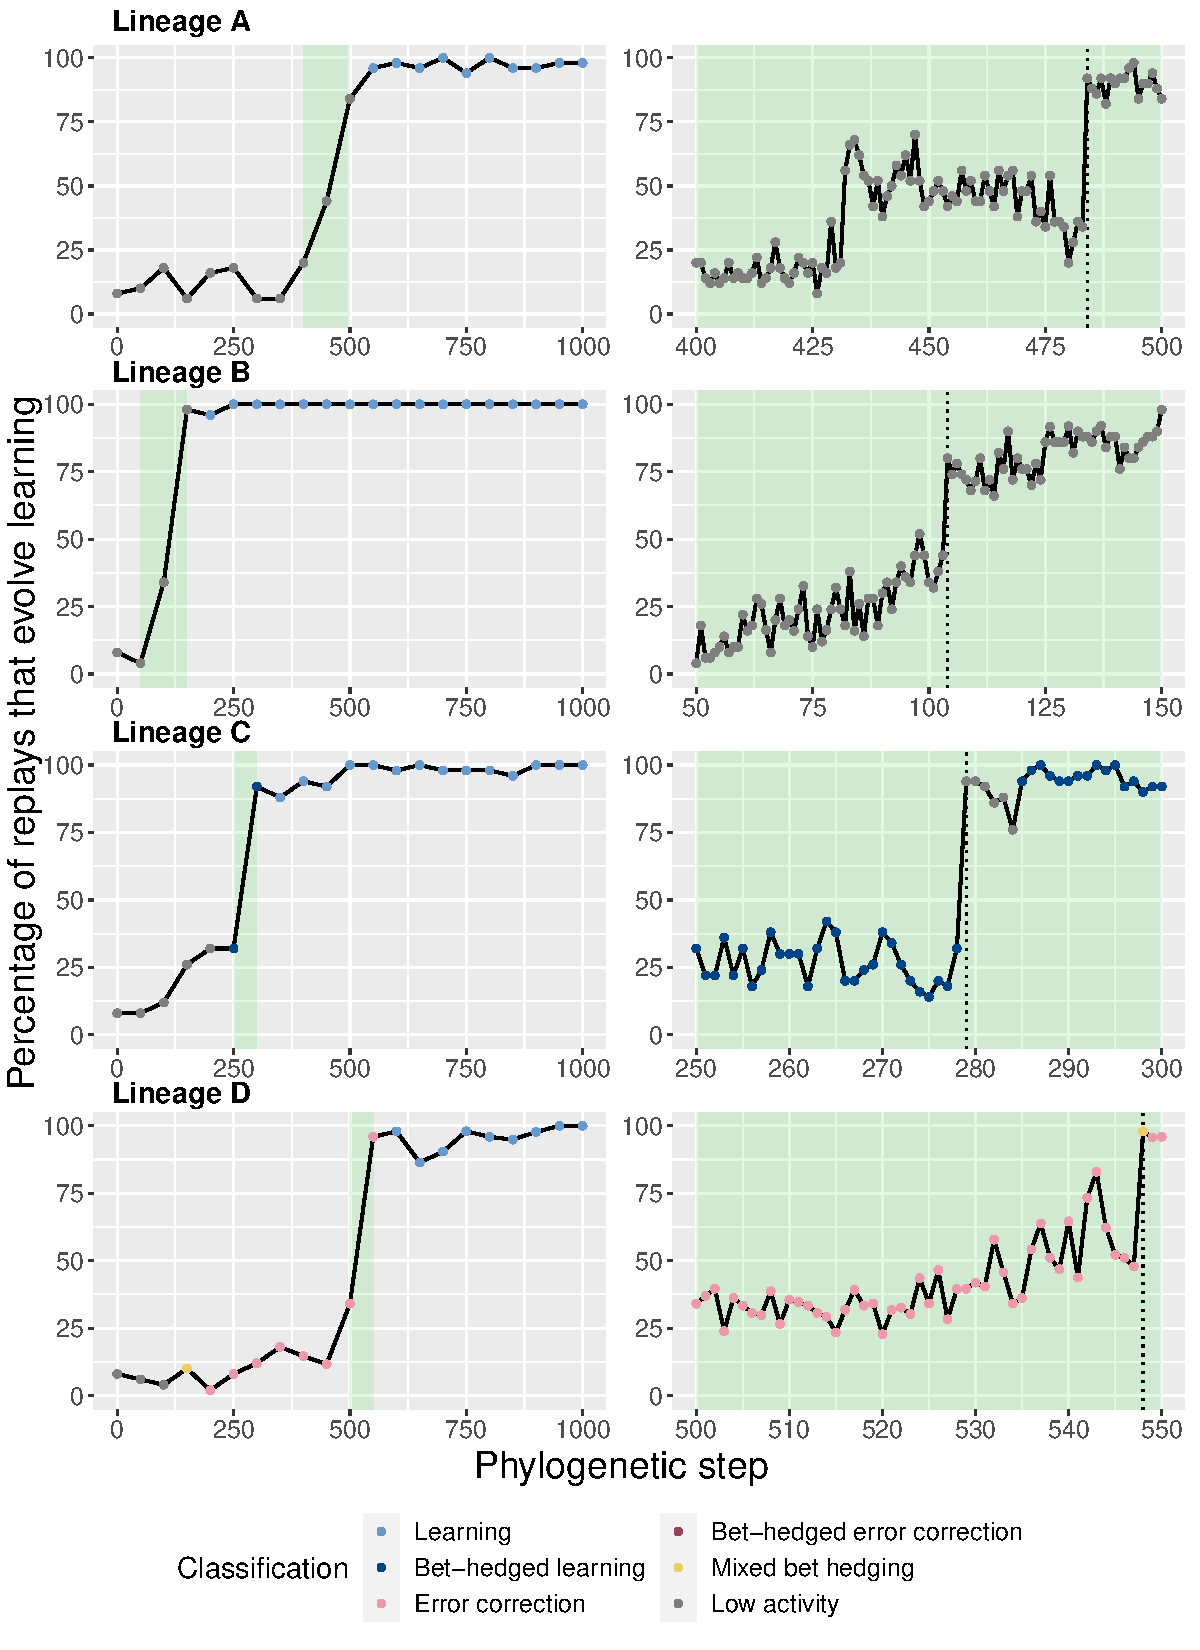
\includegraphics[width=0.8\textwidth]{03_learning_case_studies/media/combined_replays_R.pdf}
    \vspace*{-3mm}
    \caption{
        Potentiation of associative learning for all case studies, shown as the percentage of replicates that evolve associative learning when replayed from a given genotype. %evolution is replayed starting at that point. %, as it changes over the lineage for the four case studies. 
        For each case study, the left plot shows the results of the exploratory replays. 
        We identified a window of potentiation gain in each lineage, indicated by the shaded region. 
        Within that window, we conducted targeted replays for every step along the lineage, shown on the right. 
        %The results of those targeted replays are shown in the plots on the right.
        The color of the points corresponds to the behavior exhibited at that step of the lineage. 
        A dotted line in the targeted replays indicates the step that conferred the most potentiation.
    }
    \label{fig-potentiation-all-case-studies}
    \end{center}
\end{figure*}

Below we present the results of the replay experiments performed on the four focal lineages and provide a step-by-step analysis of how key mutations altered both immediate fitness and evolutionary potential (potentiation).
Where possible, we explained how these mutations altered the underlying algorithms.
For each lineage, potentiation across both exploratory and targeted replays can be found in Figure \ref{fig-potentiation-all-case-studies}.
%Additionally, details about the most-potentiating mutation from each lineage can be found in Table \ref{tab:replay-summary}.

\subsubsection{Lineage A}

% \begin{figure}[!h]
%     \begin{center}
%     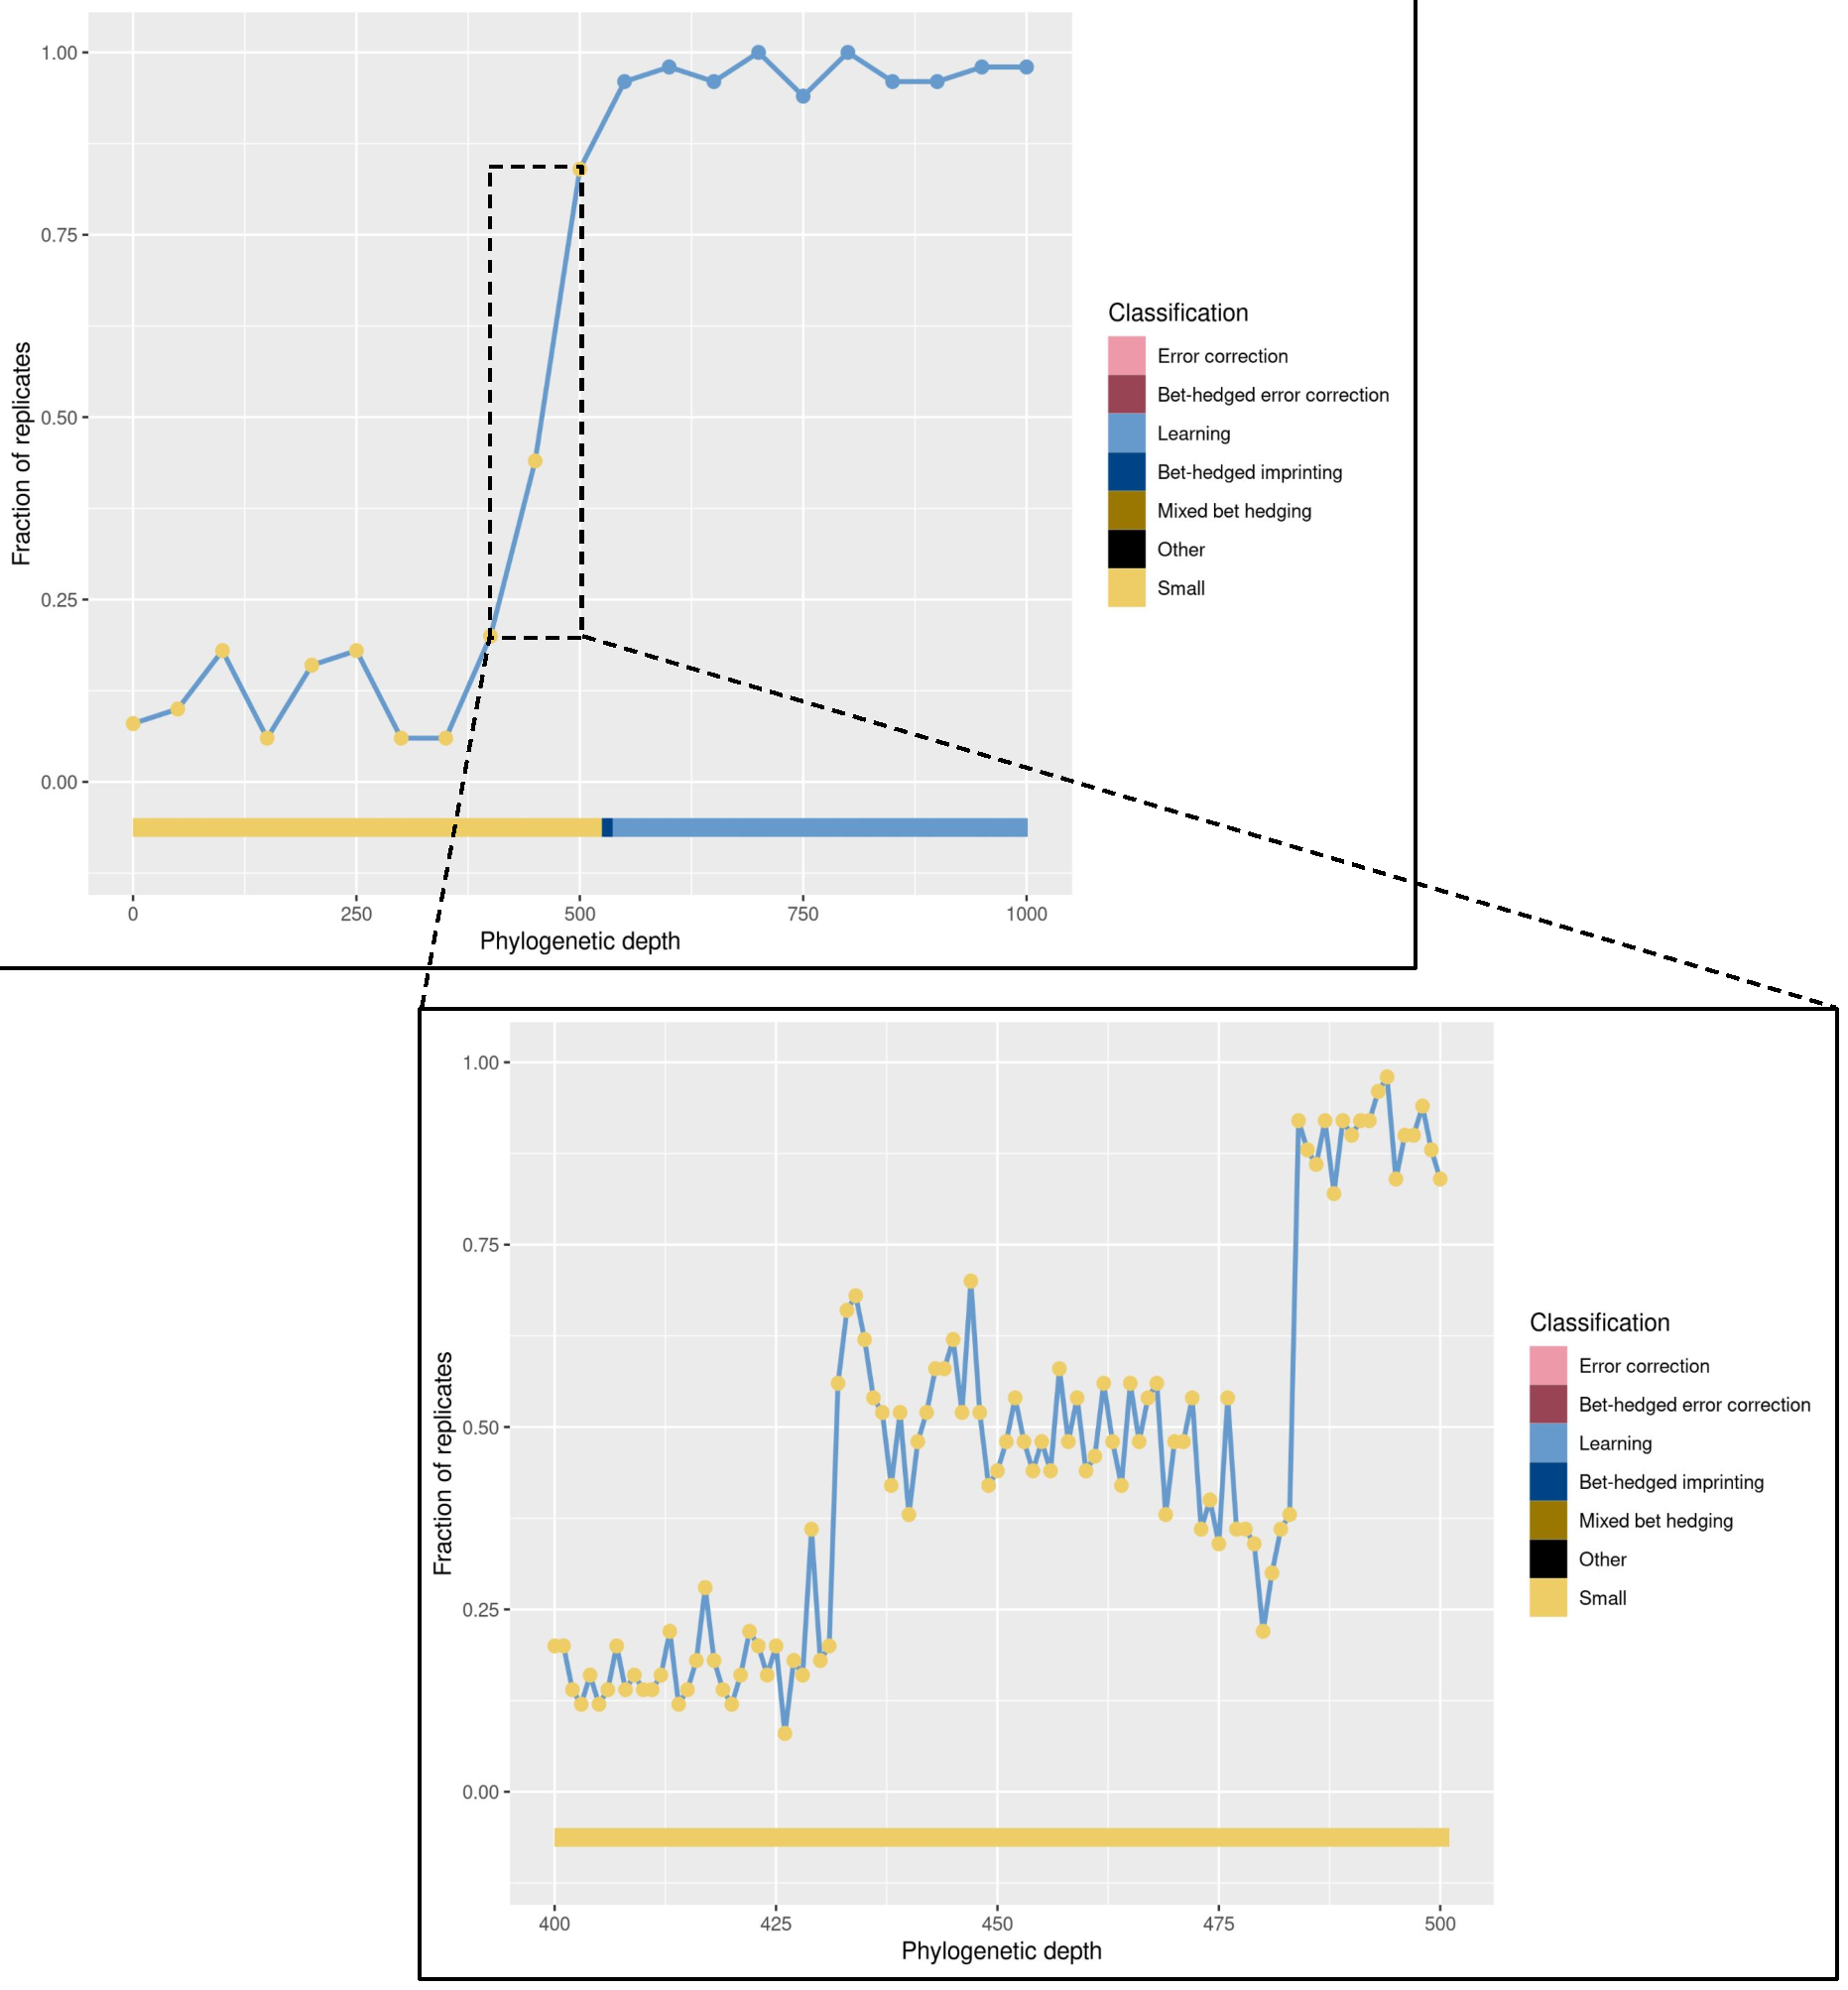
\includegraphics[width=0.45\textwidth]{media/test_pop_out_seed_86.pdf}
%     \caption{
%         \textbf{Case Study A}.
%         Potentiation of associative learning, shown as the fraction of replicates that evolve associative learning when replays are started at that point, as it changes over the lineage for Case Study A. 
%         The top figure plot shows the results of the exploratory replays. 
%         Two windows of increased potentiation were identified, indicated by the dashed rectangle. 
%         Results of the targeted replays are shown in the bottom, pop-out plot.
%         Both lines and points show potentiation at various steps along the lineage. 
%         The color of the points corresponds to the behavior exhibited at that step of the lineage.
%         The rectangle at the bottom of the plot also shows the behavior at the lineage, but with more detail than the evenly spaced points of the exploratory replay.
%     }
%     \label{fig-potentiation-case-study-a}
%     \end{center}
% \end{figure}

Our first case study is one of the shortest lineages and it contains a quick jump to learning (at step 537) from low activity, with only a brief time spent in bet-hedged learning. 
%The exploratory and targeted replays for Case Study A are both shown in Figure \ref{fig-potentiation-case-study-a}.
Exploratory replays for this lineage revealed a stark jump in potentiation between 400 and 500 steps from the ancestor, which we call the potentiation window.
From step 400 to step 450, potentiation increased from 20\% of replicates to 44\%, and increased again to 84\% of replicates by step 500. 
Before this window, potentiation fluctuated around the original 8\% found starting from the default ancestor.
%Before this jump, the potentiation fluctuates between 6\% of replicates and 20\% of replicates evolving learning. 
After the selected window, potentiation increased once more and then fluctuated between 94\% and 100\%. 

With this in mind, we seeded 50 replays for each genotype in the potentiation window. 
%Since we run 50 replicates at each step, there is considerable noise in the data. 
%Regardless, two mutations confer drastic increases in potentiation: steps 432 and 484. 
Even with the noise due to a small sample size, %that comes from having only 50 replays at each step,
we identified two mutations that conferred sizable increases in potentiation: steps 432 and 484.
The mutation at step 432 brought potentiation above 50\% for the first observed time in the lineage. 
Surprisingly, potentiation then decreased (on average) back to a local minimum of 20\% of replicates at step 480. 
Finally, the mutation at step 484 substantially increased potentiation to 92\%, where it stayed for all subsequent replays. 
%Looking at performance averaged over 100 trials, both mutations are neutral in fitness.

Even though the largest jump in potentiation occurred at step 484, learning did not appear in the lineage until step 537. 
That said, only steps 516 and 525 caused any change in behavior; all other interim mutations occurred in unexecuted regions of the genome. 
The potentiating mutation at step 484 made a key instruction in the main loop of the genome redundant.
It had no immediate effect on fitness, but later (in intermediate step 516) allowed the redundant instruction to be replaced by
%, mutating the redundant instruction into 
a right turn that granted a small fitness increase as organisms could now navigate until they reached the second left turn. 
Step 525 further improved navigation, but used a comparison that made an unfounded assumption on whether the left or right random cue is larger. 
When the assumption was correct organisms were capable of learning the cues, however the assumption is only correct 50\% of the time, so this genotype is categorized as bet-hedged learning. 
Finally, step 537 swapped that comparison with one that makes no assumptions about cue values, enabling the genotype to learn in all environments. %and now the genotype can always learn. 

Looking at the local mutational neighborhood, the potentiating mutation at step 484 increased the number of two-step mutations that conferred learning from 2 to 9 (of approximately 56 million). 
Additionally, the fitness of the learning mutations in the local neighborhood increased by three or four orders of magnitude.
%Specifically, the mutation at step 484 adds a \texttt{Decrement} instruction at the very first position in the genome. 
%This makes another \texttt{Decrement} instruction in the midst of the main section of the genome obsolete, as it was only called once and now is never called because of the new mutation. 
%With that locus now free to mutate, step 516 sees a mutation at that exact locus, swapping it to a \texttt{Right} movement instruction.
%This allows organisms to move right for the first time, which they do successfully a few times before being stumped by a \textit{left} immediately followed by a \textit{right}.
%Finally, the mutation to learning at step 537 adds more flow control before the new \texttt{Right} instruction, alleviating the issue and allowing organisms to cleanly handle any sequence of states. 
%These three mutations saw a shift from less than 7 correct states, on average, at step 484, to less than 10 at step 516, to over 115 at step 537, resulting in a drastic fitness increase.
%While was purely neutral in fitness when it occurred, the mutation at step 484 shifted the genetic material to allow changes to the vital machinery and paving the way for learning. 

What about the earlier potentiation that was gained and then lost?
The mutation that substantially increased potentiation at step 432  introduced a comparison that had no immediate fitness effect. 
This comparison remained unimportant until step 525 when it became integral in introducing bet-hedged learning. %interacted with that new comparison to improve the algorithm. 
%Looking at two-step mutations, neither step 432 nor the step before had any learning in their local landscapes. 
Neither step 432 nor its predecessor had access to learning within a two-step mutational range.
Thus, it is likely that the potentiation comes from that comparison given that we observed it being utilized for learning later on.

%The earlier potentiation at step 432 swapped a \texttt{Push} instruction for an \texttt{IfLess} instruction. 
%At the time, this did nothing. 
%In fact, this instruction only comes into play at step 537, where it becomes part of the logic of ``if B does not equal C AND C is greater than or equal to 3, then take a right turn''. 
%Thus, while it took a while to get there, the mutation was directly useful in the learning algorithm. 

%[MOVE TO DISCUSSION???]
Why then, did potentiation decrease between steps 432 and 484?
At step 432 (and indeed before it), the algorithm had a section where if register B was non-zero, then B stored the cue associated with a left turn. 
While this information was likely to make the evolution of learning easier, it was unused at that time. 
As such, the mutations between steps 432 and 484 dismantled that machinery, requiring a replacement to be built before learning could evolve.

%increasing the number of mutations needed for learning to evolve. 
%Indeed, this machinery was rebuilt before learning evolved, but in a different way. 

\subsubsection{Lineage B}

% \begin{figure}[!h]
% \begin{center}
% 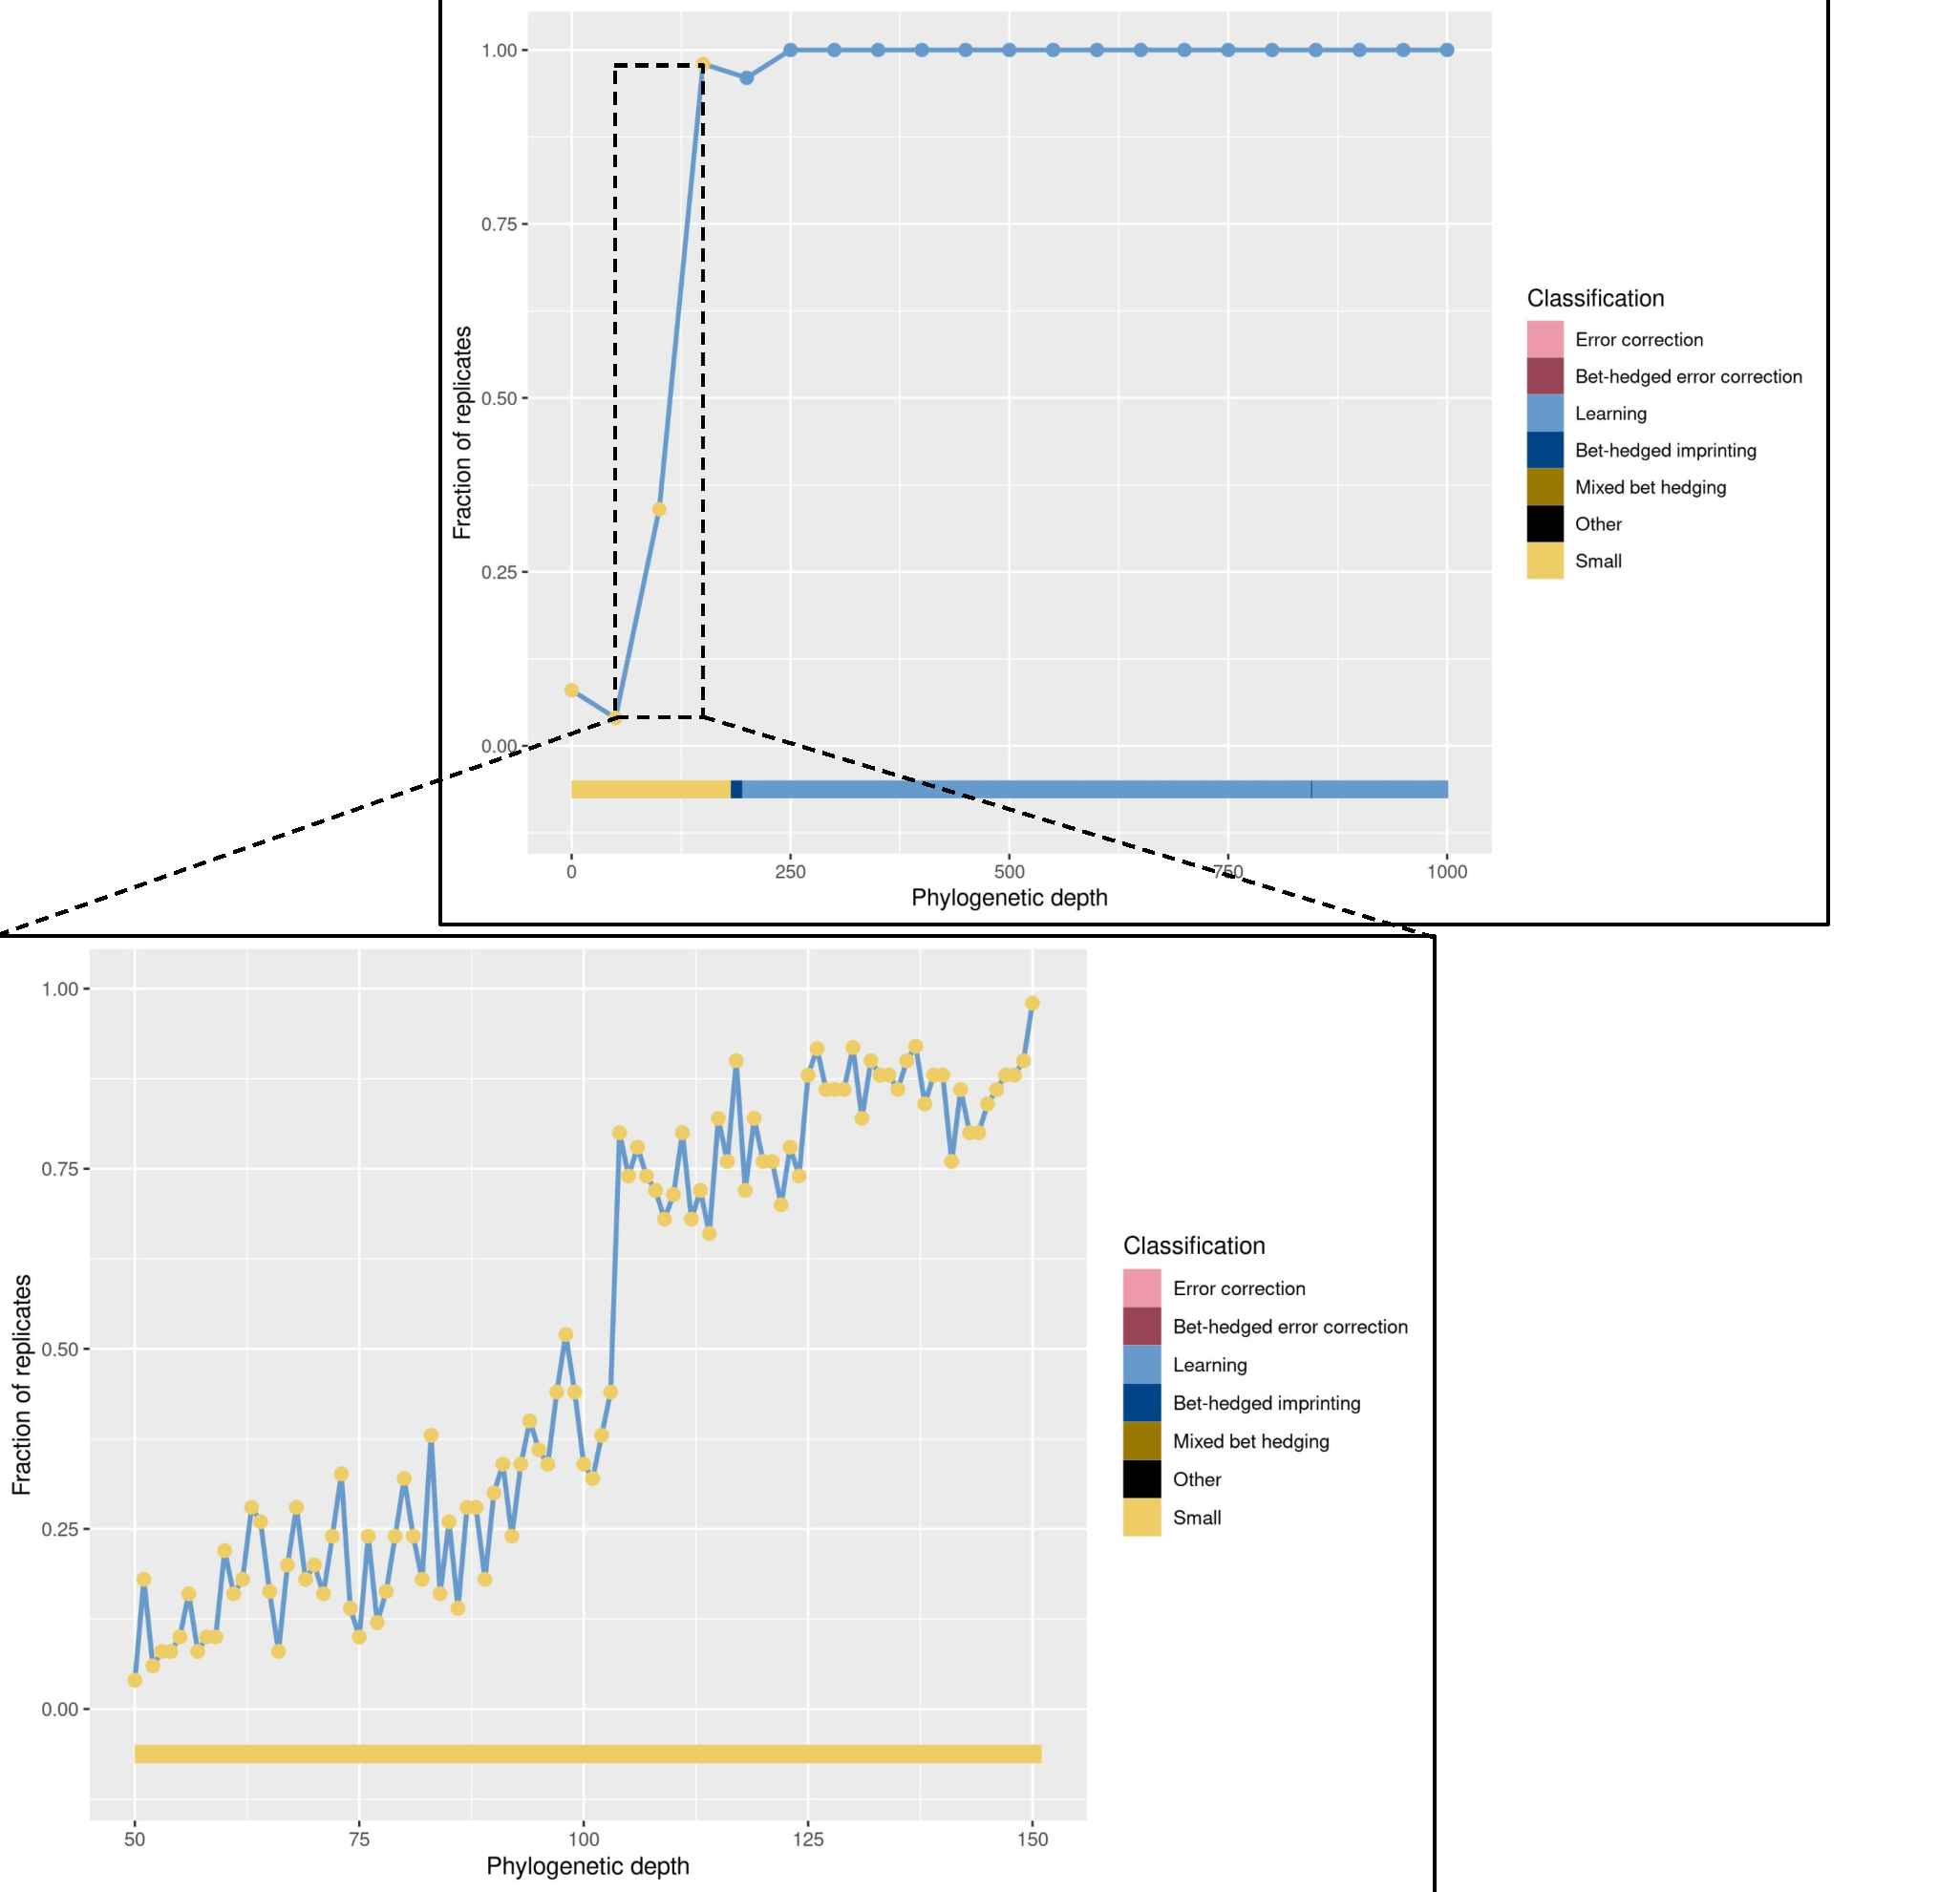
\includegraphics[width=0.45\textwidth]{media/test_pop_out_seed_4.pdf}
% \caption{
% \textbf{Case Study B}.
% Potentiation of associative learning as it changes over the lineage for Case Study B. 
% The top figure plot shows the results of the exploratory replays. 
% Two windows of increased potentiation were identified, indicated by the dashed rectangle. 
% Results of the targeted replays are shown in the bottom, pop-out plot.
% Both lines and points show potentiation at various steps along the lineage. 
% The color of the points corresponds to the behavior exhibited at that step of the lineage.
% The rectangle at the bottom of the plot also shows the behavior at the lineage, but with more detail than the evenly spaced points of the exploratory replay.}
% \label{fig-potentiation-case-study-b}
% \end{center}
% \end{figure}

Similar to Lineage A, this lineage transitioned from low activity to learning through a brief period of bet-hedged learning. 
Exploratory replays on this lineage reveal that learning was potentiated almost immediately; by step 150 potentiation had climbed above 95\%, where it stayed for the rest of the lineage. 
%From this exploration we identified 
As such, the potentiation window included steps 50 through 150. %, and therefore targeted that windows for additional replays. 

Unlike Lineage A, the targeted replays reveal a general trend of increasing potentiation, with step 104 as a notable outlier. 
%However, one mutation stands out as an outlier: step 104. 
Mutations from steps 50 through 103 slowly increased potentiation from 4\% to 44\%, but the mutation at step 104 jumped to 80\%. 
From there, another slow increase continued to raise potentiation to a peak of 98\% at step 150.

Learning did not appear until step 195, over 90 steps beyond the largest potentiating mutation. 
Given that 34 intermediate mutations altered the encoded algorithm, the mechanistic pathway to achieve learning is more complicated than can be broken down in this work.
%breaking down the exact details of the changes to reach learning is beyond the scope of this work. 
However, the potentiating mutation at step 104 modified the execution flow of the genome, which appears to have been essential for the later evolution of learning. % in the long term. 

While two mutations occurred at step 104, only one caused a functional change: an instruction to swap data between registers was mutated to a left turn. 
Prior to this mutation, the genome encoded a left turn later on, after which the execution became trapped in an endless loop. 
The potentiating mutation was immediately beneficial; it allowed organisms to take the left turn earlier, which, in turn, allowed them to avoid the loop. 
%As such, this mutation was immediately beneficial when it occurred.
As a side effect, a large portion of the genome that was previously executed was now skipped, and these instructions remained skipped when learning evolved 91 steps later.
%In avoiding the infinite loop, a large portion of the genome was now skipped and remained so when learning evolved 91 steps later. 
Looking at the local fitness landscape, learning was neither present in the potentiating step's landscape nor in the step before.
We hypothesize that the potentiation came from the change in execution flow, and that skipping over those instructions avoided a pitfall and freed up execution time that may have been useful in evolving learning.

%While two mutations occurred at step 104, only one provides a functional change. 
%That mutation is a point mutation swapping a \texttt{Swap} instruction for a \texttt{Left} movement instruction. 
%Another \texttt{Left} instruction already existed a little further along the genome, but removing the \texttt{Swap} instruction allowed execution to jump back to the main portion of the genome, while still executing the needed left turn before doing so. 
%This increased fitness immediately, as it prevented the organism from getting stuck in an infinite loop at toward the end of the genome, instead correctly handling a few more states. 
%Secondly, this caused a large portion of the genome to not be executed, most of which is still skipped when learning evolved at step 195. 
%The mutation at step 104 did prove important, as it persisted throughout evolution, being present in the final genome at step 1544.


\subsubsection{Lineage C}

Lineage C has the biggest single-mutation potentiation increase (64 percentage points), and that mutation was deleterious when it occurred at step 279 along the lineage.  
Learning later appeared at step 305. 

The potentiating step mutated a no-operation instruction into a conditional flow control instruction. 
%On the existing genetic background, this mutation was terrible for fitness.
At step 278 the genotype was capable of bet-hedged learning, but the mutation at 279 knocked out all instances of learning, reclassifying the behavior as ``low activity.'' %down below the classification threshold. 
The next step restored some fitness, and then step 285 interacted with the mutation at 279 to not only restore fitness, but to dramatically improve it. 
Ultimately, the potentiating mutation at step 279 allowed the algorithm to more precisely discriminate between the left and right cues. 
%Prior to the mutation, a less-than comparison was used, which only functioned correctly in instances where the \textit{left} cue was less than the \textit{right} cue; this assumption was only valid half the time, resulting in the bet-hedged learning seen before the potentiating mutation. %left the algorithm at the mercy of the random cue values. 
Prior to the mutation, a less-than comparison was used, which only functioned correctly in 50\% of instances, specifically those where the \textit{left} cue was less than the \textit{right} cue. 
%This assumption resulted in the bet-hedged learning seen before the potentiating mutation.
%The potentiating mutation switched it to an equality comparison, which alleviated the assumption and paved the way for learning in all instances. %that one cue will be larger than the other.
The potentiating mutation switched to an equality comparison, which alleviated the assumption and initiated the transition from bet-hedging to learning. %that one cue will b

Interestingly, the potentiating mutation lowered both the number and average fitness of learning mutations available in the local fitness landscape, % and decreased the average fitness of the learning mutants that do exist. 


% When learning appears at step 305, it comes in the form of a \texttt{Decrement} instruction being swapped for a \texttt{Subtract}.
% These genotypes cannot fix their mistakes, they rely on never making errors. 
% Steps 285 through 304 cannot handle two \textit{left} states in a row, but step 305 can. 
% By using subtraction instead of decrement, the algorithm is able to always zero out the register, which combines with the flow control and ensures the algorithm can handle multiple left turns in a row.



% \begin{figure}[!h]
% \begin{center}
% 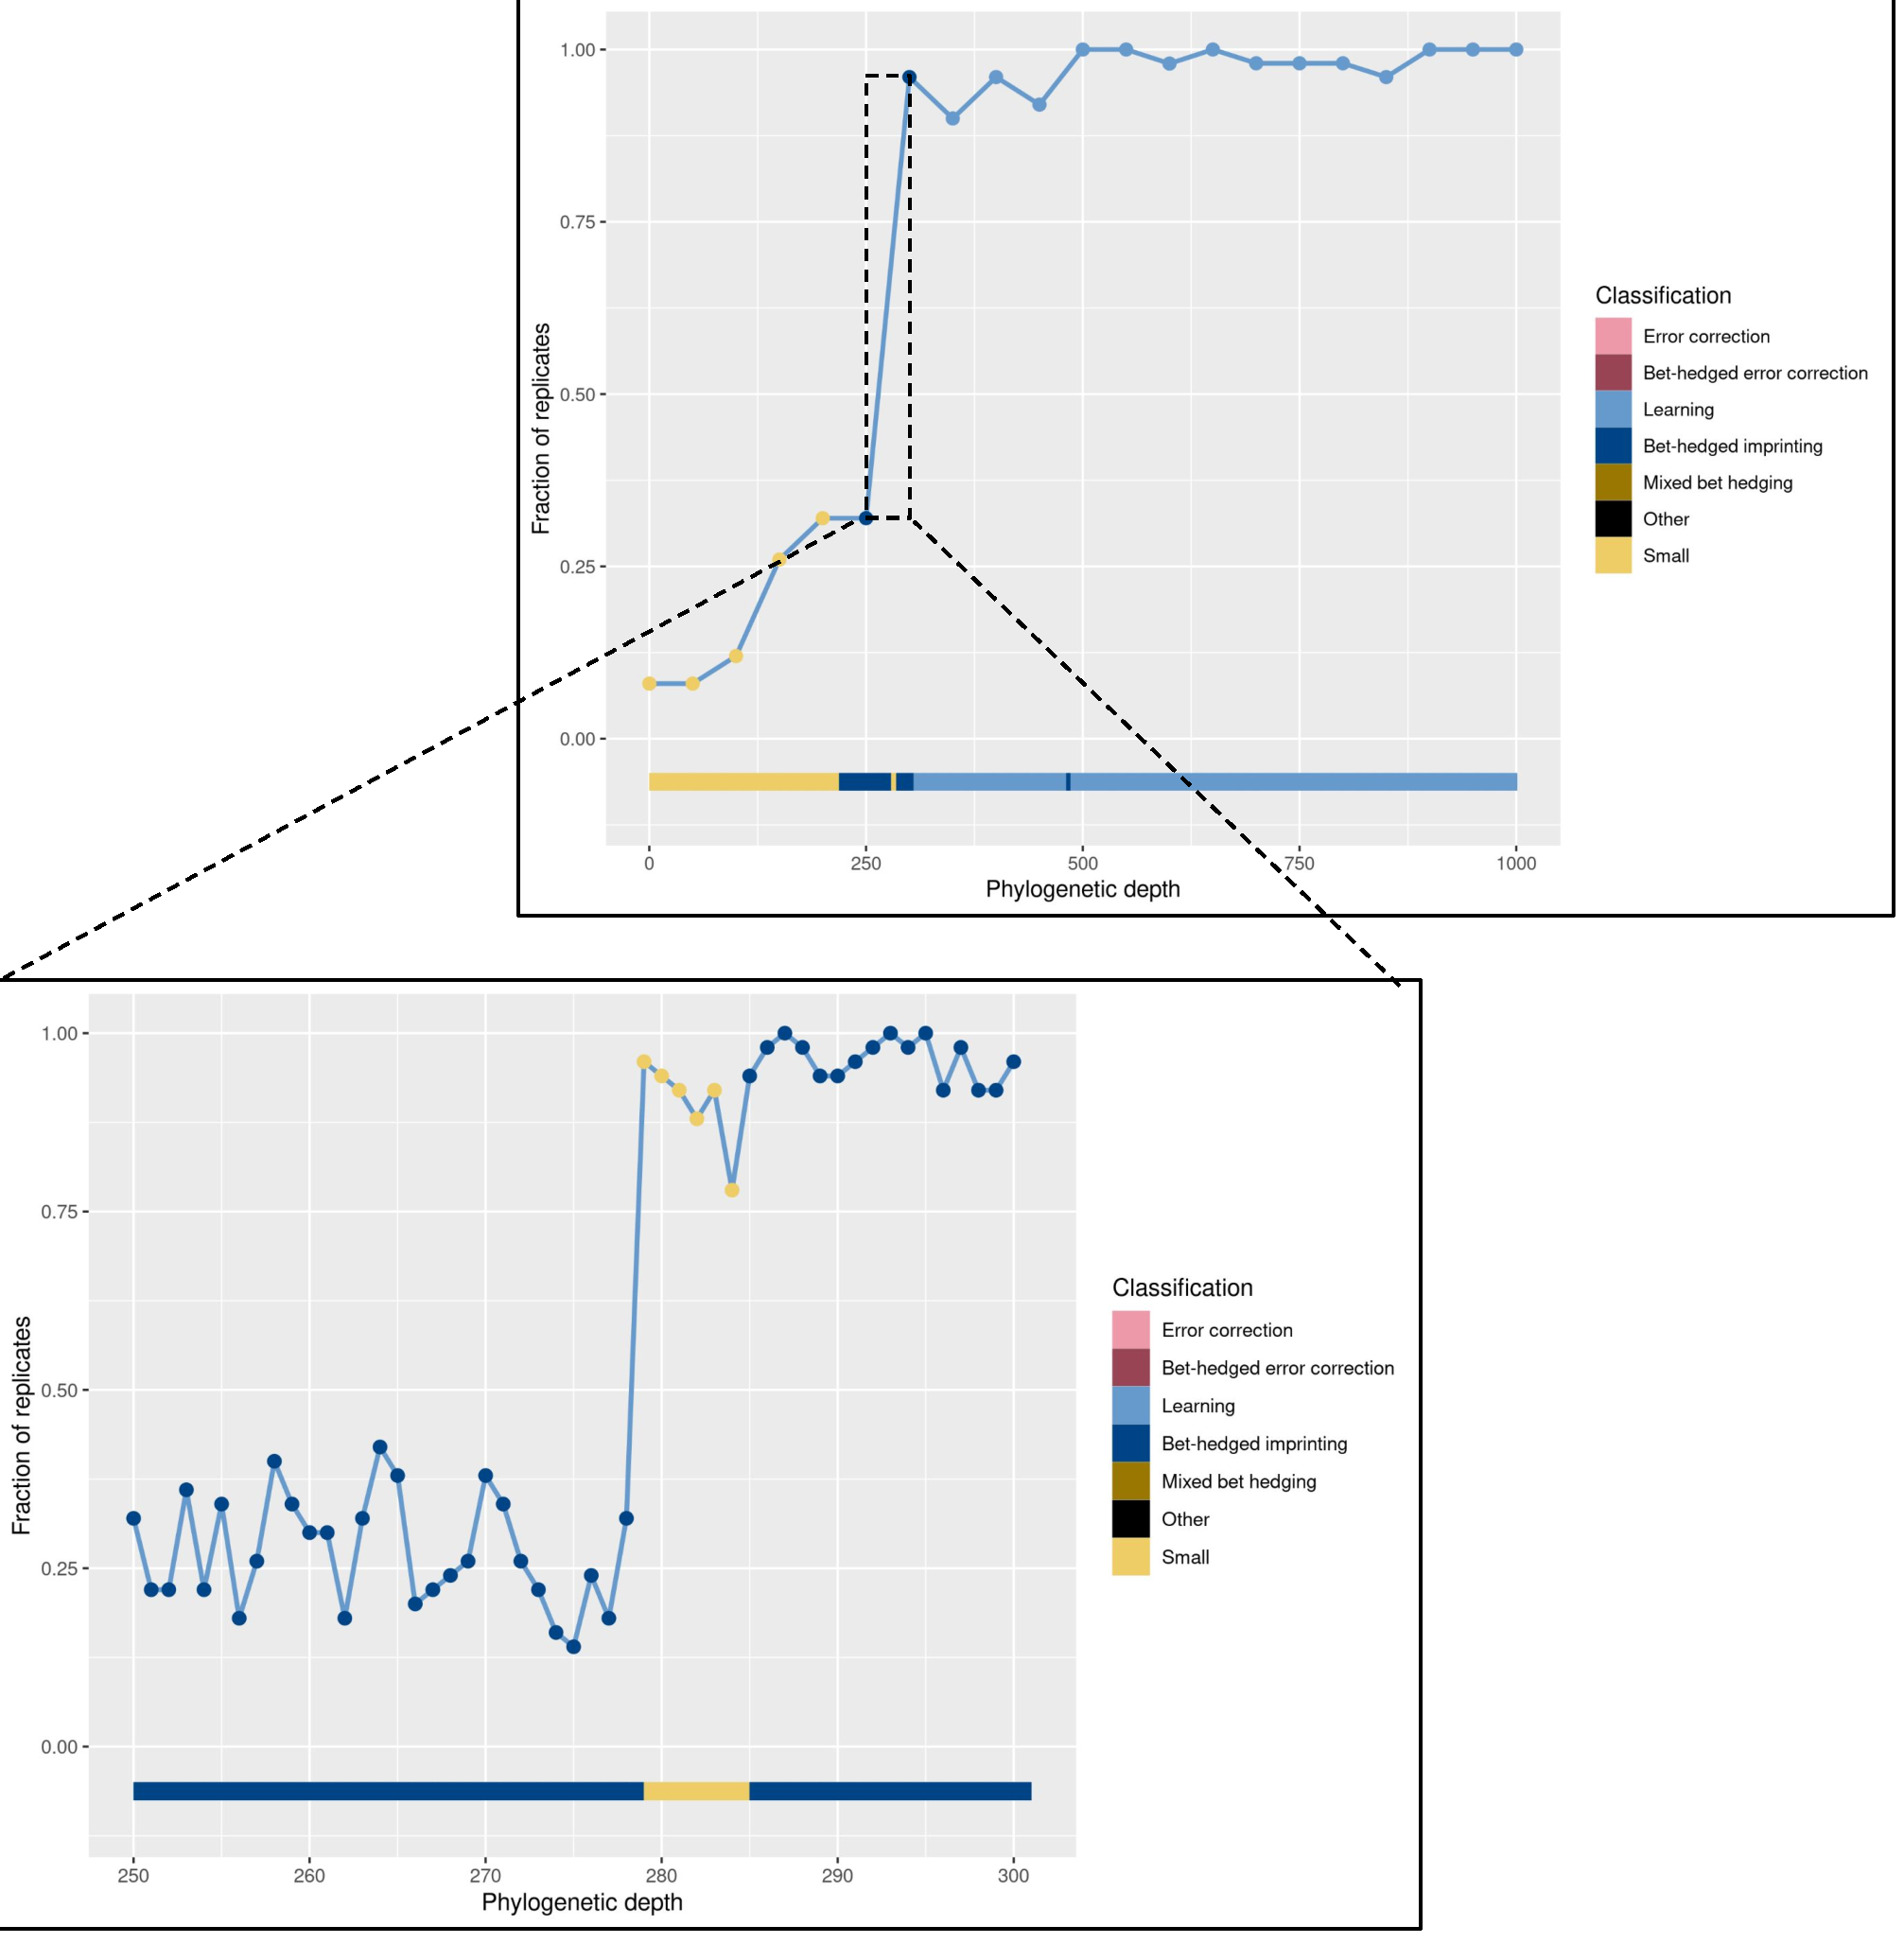
\includegraphics[width=0.45\textwidth]{media/test_pop_out_seed_15.pdf}
% \caption{
% \textbf{Case Study C}.
% Potentiation of associative learning as it changes over the lineage for Case Study C. 
% The top figure plot shows the results of the exploratory replays. 
% Two windows of increased potentiation were identified, indicated by the dashed rectangle. 
% Results of the targeted replays are shown in the bottom, pop-out plot.
% Both lines and points show potentiation at various steps along the lineage. 
% The color of the points corresponds to the behavior exhibited at that step of the lineage.
% The rectangle at the bottom of the plot also shows the behavior at the lineage, but with more detail than the evenly spaced points of the exploratory replay.}
% \label{fig-potentiation-case-study-d}
% \end{center}
% \end{figure}




\subsubsection{Lineage D}

% \begin{figure}[!h]
% \begin{center}
% 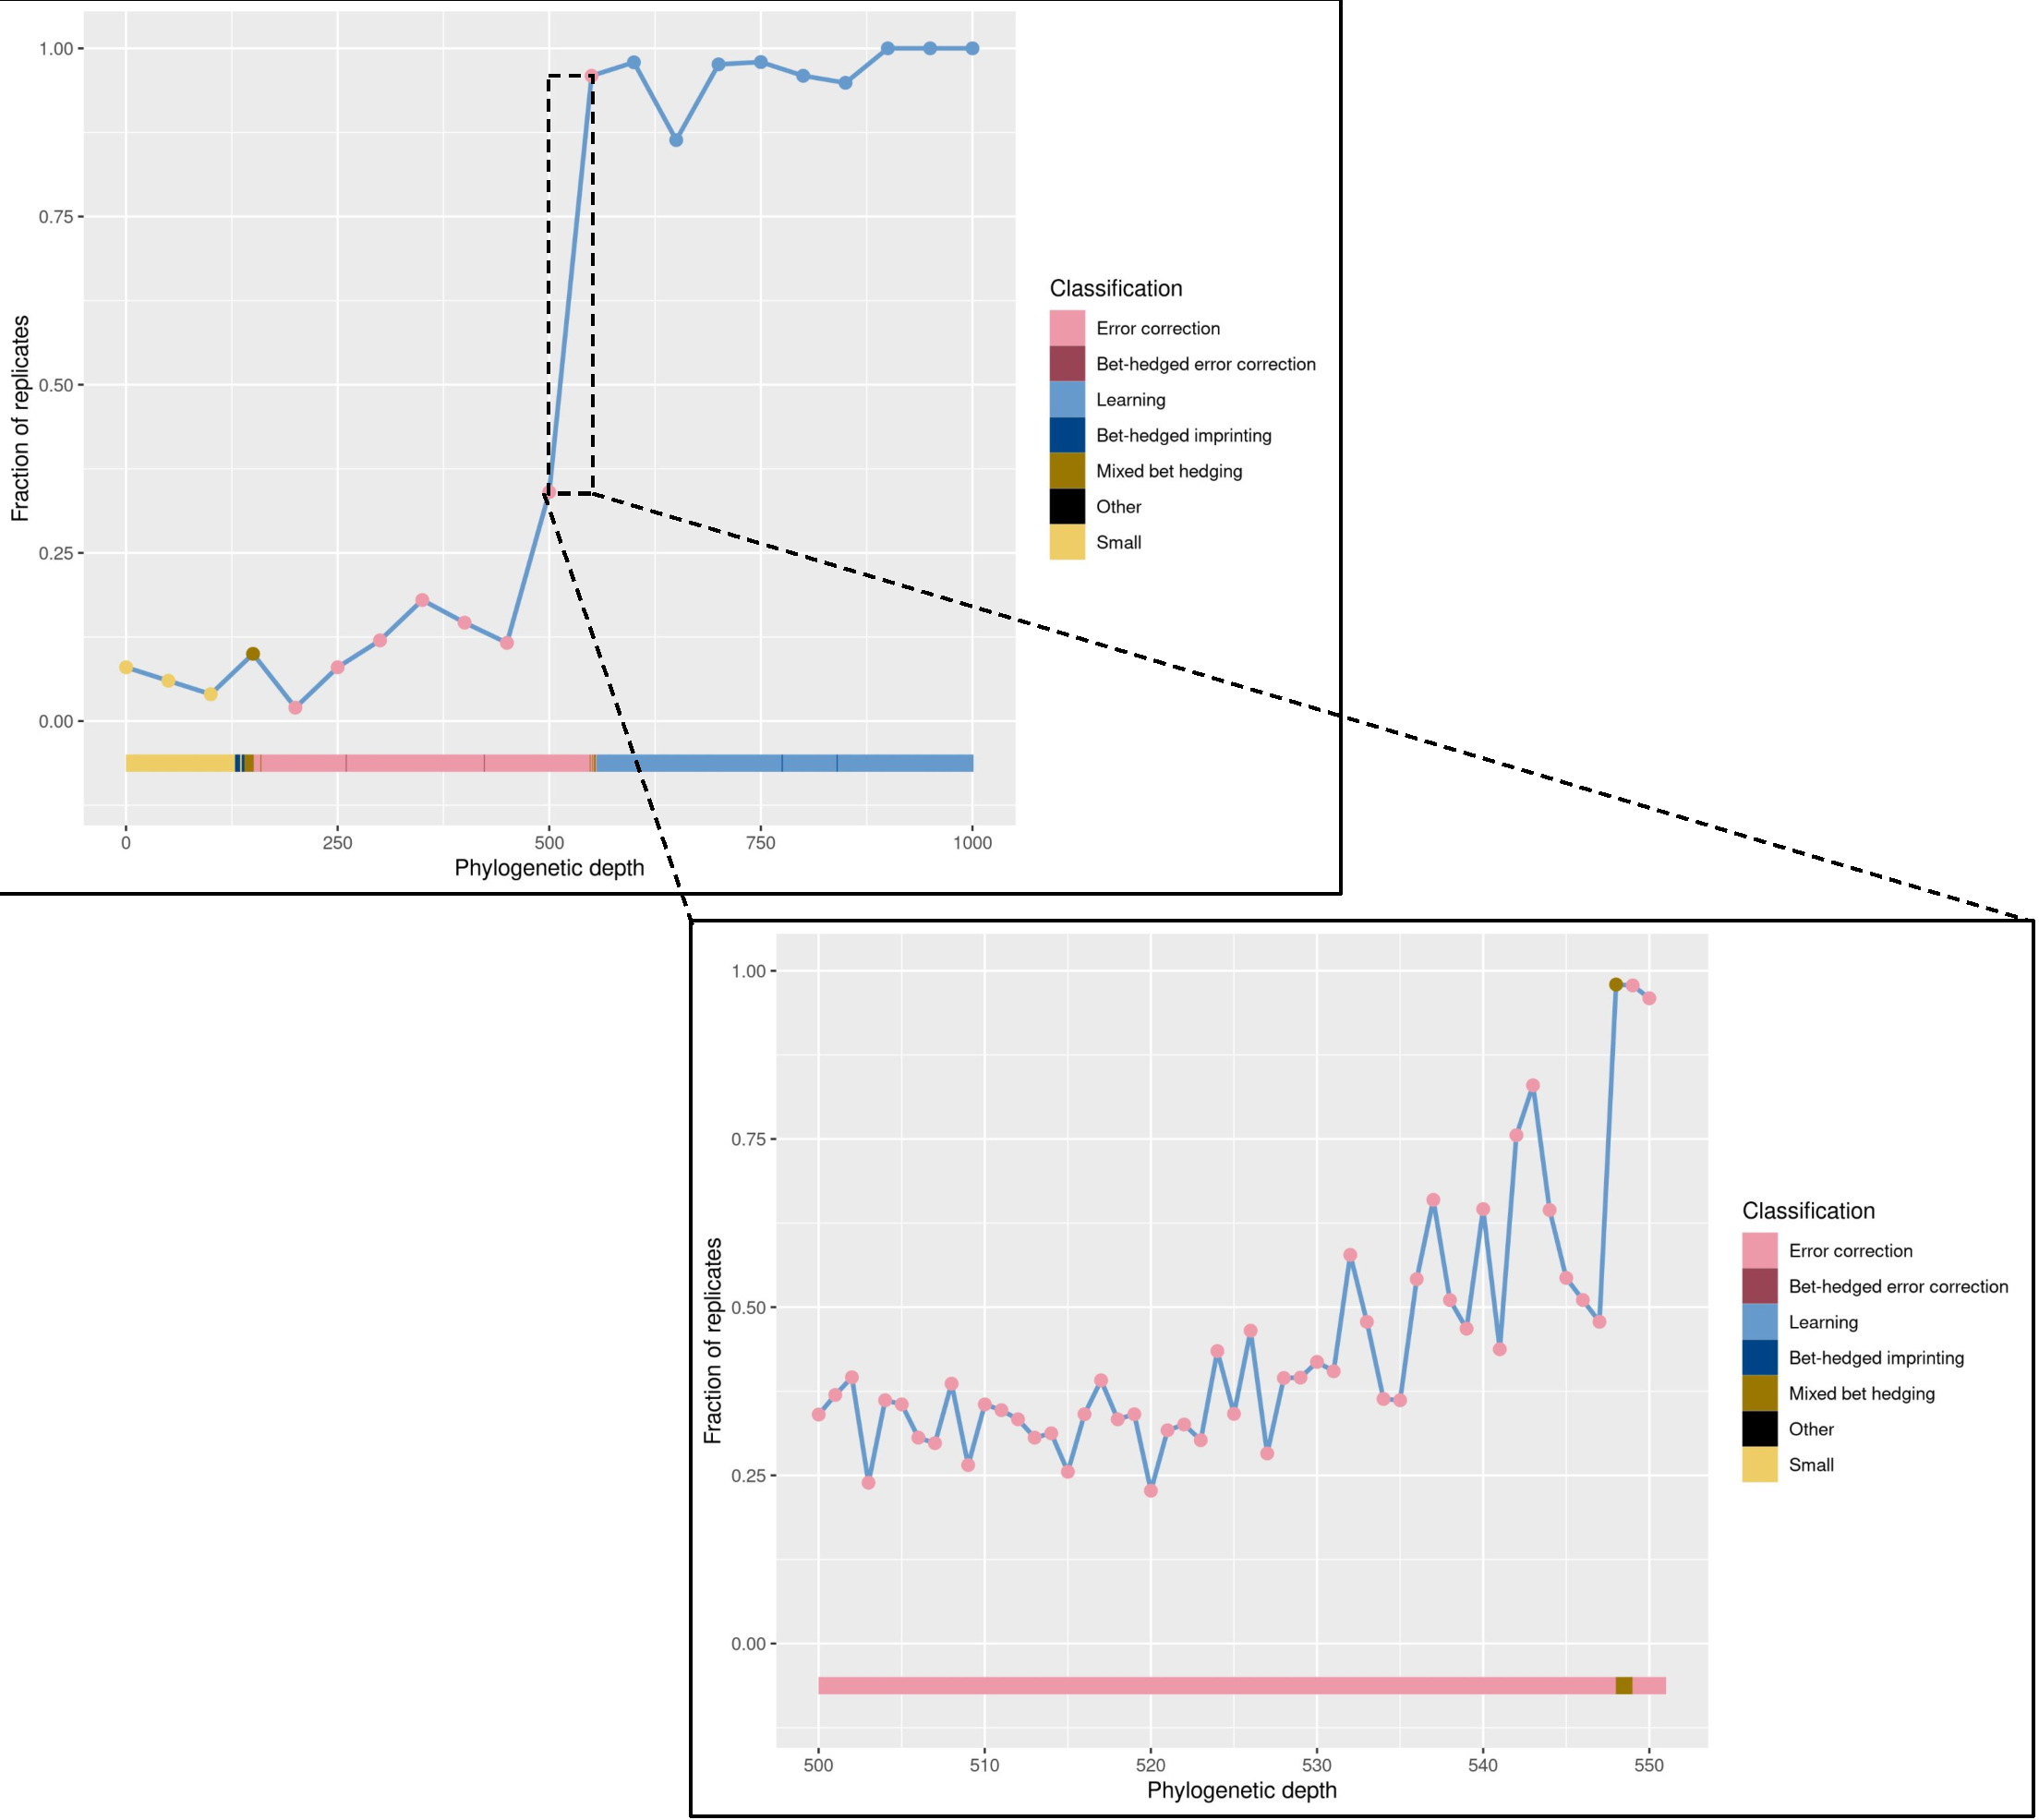
\includegraphics[width=0.45\textwidth]{media/test_pop_out_seed_6.pdf}
% \caption{
% \textbf{Case Study D}.
% Potentiation of associative learning as it changes over the lineage for Case Study D. 
% The top figure plot shows the results of the exploratory replays. 
% Two windows of increased potentiation were identified, indicated by the dashed rectangle. 
% Results of the targeted replays are shown in the bottom, pop-out plot.
% Both lines and points show potentiation at various steps along the lineage. 
% The color of the points corresponds to the behavior exhibited at that step of the lineage.
% The rectangle at the bottom of the plot also shows the behavior at the lineage, but with more detail than the evenly spaced points of the exploratory replay.}
% \label{fig-potentiation-case-study-d}
% \end{center}
% \end{figure}

Of the four replicates we analyzed, Lineage D is the only one that evolved error correction before learning.
Like the earlier lineages, the exploratory replays show that almost all potentiation comes from a single window. 
%Here, however, we only study the back half of the window, where 
In this case, potentiation grew from 34\% of replicates to 96\% between steps 500 and 550.
%Zooming in via targeted replays, potentiation in this window tells an interesting story. 
%It is hard to be certain given the noise of using 50 replay populations, but it appears that potentiation generally increases in the second half of the window. 
Targeted replays are especially noisy for this lineage, but generally show an increase in potentiation, especially in the latter half of the window.
%Of particular note are the last \~10 steps in this window. 
The largest jump in potentiation occurred at step 548, near the end of the window.
%Looking backward, however, other 
Several prior mutations also showed notable potentiation increases, but in each case later mutations appeared to counteract them. %lower potentiation again. % before later mutations lowered it again. 
Specifically, steps 542 and 543 appear to have higher potentiation than the points around them, but potentiation dipped back below 50\% before the largest jump at 548.

Out of all four lineages, D has the fewest steps between the largest potentiating step (548) and the first appearance of learning (556).
At the time, the potentiating mutations at 548 caused no discernible change in fitness even though they increased potentiation by 50 percentage points. 
Two mutations occurred at step 548: a point mutation swapped a flow control instruction for a math instruction and an insertion mutation added a comparative conditional instruction into the main execution loop. 
At step 548 the genotype encoded a naive error correction algorithm: after setup, organisms could always handle \textit{right} states, but always failed \textit{left} states, recovered, and then continued. 
%This changed when learning evolved 
%At step 556, the algorithm started sensing the environment, albeit \textit{too} often. 
A mutation at step 556 swapped a sensing instruction with a math instruction, and this combined with the prior comparison instruction from step 548 to allow the organism to move left when needed and shifted the behavior to learning.
%The organism still blundered when it encountered a state sequence of \textit{left}, \textit{forward}, \textit{left}, but it quickly recovered. 
%Since it can associate the cues with greater than 90\% accuracy, we classify it as learning. 
The local fitness landscape supports the idea that the comparison instruction was useful to the evolution of learning, as the potentiating mutation increased the number of learning genotypes in the two-step mutational neighborhood from under 800 to over 100,000.

% What's going on at 542/543?
Looking back at the apparent false start at steps 542 and 543, it is not clear what algorithmic changes these mutations conferred.
%, the potentiation mutations at steps 542 and 543 also altered 
These steps did, however, alter the set of learning behaviors that fell within the local mutational neighborhood. 
At step 541, there were only 324 two-step mutations that conferred learning, and only three of those resulted in a substantial fitness increase (a metabolic rate $> 10^{15}$). %; the merit of the best-performing mutant is ~$1.6e21$.
After steps 542 and 543, that number rose such that over 900 two-step mutations could confer learning, with over 500 resulting in a substantial fitness increase (including over 200 that reached a merit $> 10^{25}$).
We may be unsure of the exact effects of these mutations on the mechanics of the algorithm, but the changes in the local fitness landscape are profound. %to include learning algorithms with much higher fitness.


\section{Discussion and Conclusion}

%\subsection{Some mutations are potentiating.}
\subsection{Potentiation can rise suddenly}

% What evidence do we have?
We have documented several cases where single mutations dramatically increased the probability of associative learning later evolving. %arising in the longer term.
Of the four lineages analyzed, each had a single step in the lineage that resulted in a substantial increase in potentiation (ranging from 36 to 64 percentage points). 
Indeed, two of the lineages had an additional potentiating mutation that resulted in an increase of over 30 percentage points.
Looking only at exploratory replays, each lineage has a 50-step window that resulted in a potentiation increase of at least 40 percentage points.

% What does this mean?
% What does the literature say about potentiation?
While four lineages are insufficient to make any strong claims, these results demonstrate that it is \textit{possible} for single mutations to drastically increase potentiation, and provide compelling evidence that they may, in fact, be common. 
In Lineages B and D, however, we do also observe regions with smaller, incremental increases in potentiation.
Further studies are clearly necessary to more fully understand the general patterns and processes by which potentiation rises across different representations and environments.
%We do not claim that all potentiation comes from one or a few mutations, simply that future work cannot disregard the possibility that a large chunk of potentiation comes from a single mutation.


%\subsection{Some mutations are anti-potentiating.}
\subsection{Potentiation can decrease along a successful lineage}

In two of the lineages we analyzed (A and D), we see evidence of potentiation decreasing over spans of the lineage. 
%We also see mutations that decrease the probability of associative learning appearing.  
%Specifically, Lineages A and D both see jumps in potentiation that are then lost over the next section of the lineage. 
With only 50 replay populations per lineage step, our results are noisy and it is difficult to isolate what is occurring during these periods of potentiation decline.
While we were unable to identify any ``anti-potentiating'' mutations with effects as large as the positive potentiation mutations, it is possible for a single step in a lineage to greatly decrease potentiation. 

%Future work should investigate this concept of decreasing potentiation. 
Since we limited our analyses to runs where associative learning arose in the original replicate, we did not expect a preponderance of anti-potentiating mutations, but were intrigued to see evidence of them, even if at low effect.  
%However, these mutations could exist. 
These same analytic replay experiments could be applied to lineages that failed to evolve the focal behavior, to see if potentiation of that behavior experiences sudden drops. 
Similarly, our replays targeted windows with substantial increases in potentiation; other windows would be more likely to include decreases. 
Finally, failed replays from starting points with otherwise high potentiation must have failed for a reason; they too could be used as a likely source (albeit more artificial) of anti-potentiating mutations.
%Windows that see a large decrease in potentiation are more likely to contain anti-potentiating mutations, while windows of little or no potentiation change early in a lineage have the potential of an increase and subsequent decrease of potentiation within that window.
%One hypothesis is that potentiation-decreasing mutations are beneficial when they occur, and that the instant gain in fitness comes at the detriment of long-term success of evolving the complex behavior. 

%That said, in run BLAH we do see a period of steady decline in the probability of associate learning arising, though no individual mutations has a dramatic negative effect.  
%If we were to focus our replay experiments more broadly, we expect that many of the runs that never produce associative learning may exhibit more signs of anti-potentiating mutations and we plan to investigate this further in the future.

%\subsection{Potentiating mutations vary substantially from one evolutionary lineage to another}
%[Step through the different runs and talk about how different the patterns are.  Can even look at some of the runs that got associative learning, but we didn't zoom in on yet.]



\subsection{Potentiating mutations can appear innocuous when they first occur}

%[Step through these mutations and discuss how they have different immediate effects and nothing immediately identifies them as potentiating.  End with the question of "so, how are these mutations any different from other mutations?"  To have any chance of identifying potentiating mutations ahead of time, we must first further understand the underlying mechanisms that make them potentiating.]
We analyzed the mutational step in each of the four lineages that conferred the greatest increase in potentiation.
Of those four mutational events, two were neutral, one was deleterious, and one was beneficial. 
Even among these few replicates, there is no obvious pattern in the properties of potentiating mutations. 
Of the two neutral mutations, one made an instruction redundant while the other added a conditional instruction that had no effect when it was initially introduced. 
The deleterious and beneficial mutations both caused the execution flow to loop back earlier than it did before.
Additionally, the number of mutations between the potentiating mutation and the appearance of learning varied wildly between lineages, ranging from 8 steps up to 91.
The potentiating mutations in these four lineages are unique, and at the current time there is no pattern emerging among them.
So, how are these mutations any different from other mutations?
Untangling this mystery could be critical for predicting evolutionary outcomes or accelerating adaptive evolution.


% \subsection{What makes a mutation potentiating?}
\subsection{We can identify \textit{how} a mutation is potentiating}

There are many mechanisms by which a mutation could facilitate the evolution of associative learning.
For example, the mutation could provide a building block that is helpful to perform the task.  
But for a mutation to be potentiating it must notably increase the probability of associative learning appearing in the future.
Any change, no matter how helpful, that was already likely to occur would not be considered potentiating.
Indeed, it is the earlier mutations that made that change so likely that would be potentiating.
Of course, those mutations are also more challenging to identify.
%Here we define a potentiating mutation as one that increases the probability of associative learning eventually appearing by at least 0.25. (or 25 percentage points).

We have three different hypotheses for how a mutation could be potentiating:
% \begin{enumerate}
%     \item The mutation grants access to associative learning in the local fitness landscape (one or two mutations away)
%     \item Associative learning was available in the local landscape, but not beneficial; the mutation makes it valuable and drives evolution toward it.
%     \item The mutation is a ``gateway'' to another region of the fitness landscape.  It does not provide immediate access to associative learning, but it does grant access to a pathway to get there.
% \end{enumerate}
%(1) It moves through genetic space in a useful direction, providing access to associative learning in the local fitness landscape. % (one or two mutations away)
(1) It is the initial move into a genetic neighborhood with associative learning,
%(2) It improves the eventual value of associative learning, increasing the likelihood of the trait being selected if it does appear. % was available in the local landscape, but not beneficial; the mutation makes it valuable and drives evolution toward it.
%(2) It shifts toward the genetic neighborhoods of better versions of learning, improving potential fitness benefits.
(2) It is a shift into a genetic neighborhood with a more valuable version of learning, or
%(3) It is a ``gateway'' mutation to another region of the fitness landscape that does not grant immediate access to associative learning, but does unlock a pathway to get there.
%(3) It is a more general ``gateway'' mutation to another region of the fitness landscape, unlocking a pathway to learning that is undetectable using local neighborhood analyses.
(3) It is a ``gateway'' mutation that unlocks a beneficial pathway to learning, even though learning is not in the immediate genetic neighborhood.

Across the potentiating mutations we analyzed, we have found evidence for each of these hypotheses.
The largest potentiating mutation in Lineage D supports Hypothesis 1, as it is the first time in the lineage that learning is only one mutation away. 
The main potentiating mutation in Lineage A and the earlier potentiation mutations in Lineage D support Hypothesis 2 as both cause drastic increases in the fitness benefit of learning mutations in the two-step neighborhood. 
%It is worth noting that the mutation in Lineage A still only has a few two-step mutations with learning, while the mutation in Lineage D has many. 
Finally, Lineages B, C and the early potentiating mutation from Lineage A all provide support for Hypothesis 3. 
The mutations from Lineages A and B both have \textit{zero} learning mutations in their two-step neighborhoods. 
Interestingly, Lineage C sees a \textit{decrease} in the number and fitness of learning mutations in the local neighborhood. %and in the fitness of those learning mutations. 

Hypothesis 3 has many possible mechanisms by which it may work.  
For example, new traits may produce a single, clear, beneficial pathway of improvements to follow.  
Alternatively, a new building block may open a larger region with many different ways of evolving associative learning.
Finally, the mutation may actually damage existing functionality or remove existing interactions that were impeding further evolution.
While all three hypotheses have some support, future work can begin to uncover if a certain hypothesis is seen more often, what conditions might result in each scenario, or if additional analyses are needed to truly characterize these potentiating mutations. 

% Seed 86 - Hyp 2 - Increases number of two-step learning muts from 2 to 9, as well as a increase in fitness of 3 or 4 orders of magnitude
    % Seed 86 (earlier mutation) - Hyp 3 - No learning in local landscape
% Seed 4 - Hyp 3 - No learning in local landscape
% Seed 6 - Hyp 1 - Increase in the number of learning genotypes in the local neighborhood
    % Seed 6 (earlier mutations) - Hyp 2 - greatly increases the fitness benefit of learning (and maybe slightly increases the number of two-step mutations that have it)
% Seed 15 - Hyp 3 - Reduces number of learning genotypes, so not Hyp 1 or 2

\subsection{Outlook}
This work is only an early step, focused on developing techniques and expectations for performing fine-grained analyses of replay experiments. 
Next, we must expand beyond four lineages, to collect broader, more systematic replay data, automating as much of the process as possible.
%Naturally, looking at only four lineages has serious limitations, and conducting a study with enough data to aggregate the characteristics of potentiating mutations would be incredibly informative. 
We conducted this study on associative learning in Avida, but the underlying techniques must be examined broadly in other environments and substrates to ensure that our results are not unique to Avida or the evolution of associative learning. %to the specific task, so experiments that collect evidence more broadly are critical. 
Within the current study system, there are many questions that remain unanswered: 
We focused on large \textit{increases} in potentiation, but are there more obvious signals associated with \textit{decreases}?
How much of the noise that we see in our data is due to limiting ourselves to 50 replicates, and how much of it is do to actual shifts in potentiation with each mutation? % Are there signals we are missing due to noise?
What does potentiation look like in replicates that fail to evolve learning? %, or what does the potentiation of other behaviors look like in learning lineages?
%Additionally, we did not collect phylogenetic data on the replay experiments to save computational resources. 
Finally, it would be valuable to compare the specific evolutionary pathways the different replays take. Do they follow the same trend or do they differ?  This would allow us to understand if, for example, a potentiating mutation funnels evolution in a fixed direction.

Ultimately, these analytic replay techniques provide us with a tool for examining evolution in a prospective fashion, not just the retrospective approach that we are traditionally limited to.
They will allow for the development of new evolutionary theory and predictive capacity that will be invaluable, both for understanding how meaningful complexity is produced in the natural world and for improving evolutionary applications. 
        % Do this analysis, but at a scale that we can get aggregate data
        % Different substrates
        % Different tasks
        % Why only look at large _increases_ in potentiation? What's going on with the _decreases_?
        % What's going on with the lineages that _don't_ evolve learning?
        % Is sampling 50 replicates enough? 
            % Are we missing interesting trends?
            % Are we reading too much into noise?
        % We could also track phylogenies on the replays
            % How closely do replay lineages match to the original lineage?

%\section{Conclusion}

% Combined with Discussion

% \begin{figure}[t]
% \begin{center}
% \includegraphics[width=2.1in,angle=-90]{fig1.eps}
% \caption{``Energies'' (inferiorities) of strings in a first-order
%   phase transition with latent heat $\Delta\epsilon$.}
% \label{fig1}
% \end{center}
% \end{figure}

% \vspace*{-2mm}
\section{Acknowledgements}
We thank the reviewers and the MSU BEACON lab for comments. 
This work was supported by the U.S. National Science Foundation (DBI-0939454) and compute resources from the MSU Institute for Cyber-Enabled Research.

% \footnotesize
% \bibliographystyle{apalike}
% \bibliography{bibliographies/ferguson} % replace by the name of your .bib file


% \end{document}


%\chapter{In-progress - A deeper exploration of potentiation in associative learning}
%\chapter{Twisting Fates: Individual Mutations Potentiate the Evolution of Associative Learning}
% Evolutionary Catalysts 
% Recognizing Potential: Identiying individual mutations that catalize evolutionary outcomes.
% On the Ubiquitousness of Potentiating Mutations (in Avida)
%\chapter{The ubiquitous potentiating mutation: A large-scale study of associative learning in Avida}
%\chapter{The ubiquity of potentiating mutations: A large-scale study of historical contingency in Avida}
\chapter{A large-scale digital evolution study of historical contingencies in associative learning}

\label{chap:learning_distributions}

\noindent
Authors: Austin J. Ferguson and Charles Ofria 

\noindent This chapter is in final preparation before submission.

This chapter directly extends the previous chapter. 
We expand from analyzing the potentiation dynamics of four case study lineages to replaying 50 lineages.
With this larger dataset, we begin to conduct statistically powerful analyses of the the distribution of potentiation changes. 
In all 50 lineages we find a single-generation step in the lineage where the potentiation of associative learning increases significantly. 
Further, we verify that these increases are most often driven by a single mutation, though we do find evidence that multiple mutations can interact to increase potentiation. 
We find that these large potentiation increases are comparable to some, but not all, previous works on potentiation, and discuss those comparisons in detail. 


% \noindent
% Authors: Austin Ferguson and Charles Ofria

% \noindent
% Status: This is a direct extension of Chapter \ref{chap:alife_submission}.
% It is marked in-progress as all software has been implemented and additional explorations beyond Chapter \ref{chap:alife_submission} have been conducted to identify useful changes to parameters and the environment. 
% The actual data collection, however, has yet to begin. 
% Note that this chapter may make Chapter \ref{chap:alife_submission} redundant in the final dissertation.
% Both are included here, however, as Chapter \ref{chap:alife_submission} serves as preliminary results for this chapter. 

% Introduction
% Succinct, with no subheadings.

% What events were \textit{key} in the fall of an empire? 
% What turns solidified your victory in that board game? 
% What mutations were most important in the evolution of that behavior? 
% Alas, while these are all valid questions, the sheer number of possibilities means that we will likely never know the answers. 
% That is, unless we are talking about digital evolution, in which we have reached a point where it is computationally feasible to decypher which mutations had the largest effect on the final evolved population. 

%In the natural world, we typically see the fruits of evolution's labor. 
%Even in experimental evolution, we only see

\section{Introduction}

In Chapter \ref{chap:learning_case_studies} I conducted four case studies and analyzed the genetic potentiation of associative learning in the Avida digital evolution system. 
As in the previous chapter, here I use ``genetic potentiation'' to refer to changes in the genetic background that promote the evolution of a particular trait or behavior, in this case associative learning \citep{blountHistoricalContingencyEvolution2008}.
%In the previous chapter, 
We found that potentiation can increase over a short period of time, including a single mutation between parent and offspring. 
While I conducted a deep examination of the observed potentiation dynamics in Chapter \ref{chap:learning_case_studies}, I limited myself to examining only four case study lineages. 
Here, I expand this work by again replaying the evolution of associative learning in Avida, but shifting from detailed case studies to aggregate data by analyzing the potentiation dynamics of 50 lineages. 

My overall goal for this work is to provide a more comprehensive point of comparison for other studies on potentiation dynamics. 
While several previous studies of potentiation dynamics exist, they all analyze the dynamics of only one or at most a few lineages.
By analyzing 50 lineages, here we shift from a few data points of potentiation measurements to full distributions backed by statistically powerful conclusions. %will not have a few data points for particular potentiation measurements, but rather distribution estimates. 
With this work, I aim to accomplish two goals: 
1) to allow us to examine previous studies in a new light, possibly identifying trends in potentiation dynamics across systems, and 
2) to provide a benchmark of potentiation dynamics for future studies to compare against.

There are multiple, but not many, papers that directly or indirectly study potentiation dynamics in ways comparable to this work. 
We are testing the effect of accumulated genetic backgrounds on the subsequent evolution of a particular trait. 
Thus, we can discuss other papers that use analytic replay experiments \citep{blountContingencyDeterminismEvolution2018} to test the potentiation of a trait across different points in an evolved lineage. 
Alternatively, we can leverage mutant studies, where experimental evolution is conducted on organisms with and without a particular set of mutations, but an otherwise identical genetic background. 
However, we can only compare against studies that look at the binary categorical outcome of ``did X trait evolve?'' across replicates; we cannot directly compare to similar studies of continuous phenotypes or of evolvability \citep{woodsSecondorderSelectionEvolvability2011, travisanoExperimentalTestsRoles1995, wagenaarInfluenceChanceHistory2004}. 
In practice, you can turn a continuous variable into a categorical variable (e.g., ``did the replicates evolve a size greater than $1\mu m^{2}$''), however such analysis decisions should be made before experimentation; post-hoc analysis can unintentionally inject our own bias, thus creating a statistical skew. 

We find that, at both 50 lineage steps and single-step levels, potentiation for associative learning can increase substantially. 
Further, single-step increases in potentiation are likely to be driven by a single mutation, though we do see both epistatic and non-epistatic interactions between multiple mutations to alter potentiation. 
Finally, we compare our potentiation dynamics against other works that leverage analytic replay experiments to test the effects of actual accumulated genetic history (\citet{blountHistoricalContingencyEvolution2008}, Chapter \ref{chap:learning_case_studies}). 
Additionally, we compare against works that examine constructed one-step mutants \citep{jochumsenEvolutionAntimicrobialPeptide2016a}, or varying levels of shared history across evolutionary replicates \citep{meyerRepeatabilityContingencyEvolution2012}.
We find that several, but not all, of these other studies have observed similarly large increases in potentiation.
This result provides a baseline point of comparison for future potentiation studies, both \textit{in silico} and \textit{in vitro}.

% Materials and methods
% This section may be divided by subheadings and should contain sufficient detail so that when read in conjunction with cited references, all procedures can be repeated.

% Methods
    % Mostly the same as Chapter X
    % Changes to associative learning task
        % Fully random paths
        % Did we change the fitness exponent? (Yep, 1.25 -> 2)
        % Did we change how exit resets work? (Doesn't look like it)
    % Changes to replay framework
        % We now start at learning and work backward
        % Full population restarts instead of single org
        % Strict definition of the target window
    % Experiment design
        % Ran batches of 500 replicates until we hit 50 learning replicates
            % This took 4,000 replicates
        % For each of the 50 learning replicates:
            % 1. Run exploratory replays
            % 2. Identify targeted window
            % 3. Run targeted replays
            % 4. Analyze -- find potentiating step
            % 5. Run single-step mutational neighborhood
            % 6. Run mutation splits
        % Replay 10 non-learning replicates as a control
            % Only to the exploratory replay level
                % Record max potentiation gain / loss per window
        % Non-learning replicates?

\section{Methods}

% Overview -- this is mostly the same as the ALife paper
This work extends the study described in Chapter \ref{chap:learning_case_studies}. 
As such, most of the methods remain the same. 
At the core of these studies, we use the Avida digital evolution platform \citep{ofriaAvidaSoftwarePlatform2004a} to evolve digital organisms capable of simple associative learning in a path-following domain.  
Here we provide a brief outline of the methodology, highlighting areas where the methods differ from the previous chapter. 
All code, configuration scripts, and summarized data are available online \citep{fergusonFergusonAJReplayingEvolution2023}.

\subsection{Initial evolutionary replicates}

% How many replicates did we run?
First, we evolved populations capable of associative learning to provide lineages for us to replay. 
In order to accumulate 50 ``learning replicates'' (i.e., replicates that were capable of performing associative learning at the end of evolution), we ran batches of 500 replicates until we reached 50 learning replicates. 
This required 8 batches or 4,000 replicates total, for an ultimate success rate of $1.25\%$. 

% General Avida info -- mutation rate, pop size, etc.
The main details of these initial replicates were identical to Chapter \ref{chap:learning_case_studies}.
We started each replicate with a single Avida organism capable only of reproducing itself, and we capped the population size at 3,600 organisms by using a 60x60 grid for our population. 
We again evolved each initial replicate for 250,000 Avida updates and then identified a representative genotype -- the most abundant genotype at update 250,000 -- and extracted the genotypic lineage leading to it from the original ancestor. 
We used this lineage from each replicate to perform our replay analyses. 
Mutation rates were kept the same as the previous study: per-site substitution mutations occurred at a rate of 0.0075, while insertion and deletion mutations occurred independently at a rate of 0.05 per reproduction event. 
Organisms  were again able to replicate themselves via the \texttt{Repro} instruction, but they were still required to execute 1,500 instructions before being allowed to reproduce. 

% Re-introduce path following environment
We evaluate the organisms on the same path-following task as the previous chapter. 
At each step in the path, we provided the organisms with an integer cue indicating which action they should take to maximize their fitness (move forward, turn left, turn right, or move backward). 
Organisms must interpret the current cue and execute the correct action, with each action being a single, atomic instruction that we added to the Avida instruction set. 
The ``turn left'' and ``turn right'' cues, however, have randomized values for each organism evaluation, and as such organisms must associate the cue values with the correct actions during their lifetimes (i.e., they must encounter the cues, empirically determine their meaning, and remember them) to perform optimally. 

% What changed between that chapter and this one
This path-following environment is the same as in Chapter \ref{chap:learning_case_studies} with two exceptions: 

% Random paths
First, Chapter \ref{chap:learning_case_studies} used the pre-defined paths from \citep{pontesEvolutionaryOriginAssociative2020}, where each organism was placed on one of four ``one fixed turn'' paths. 
This configuration guaranteed that organisms would always encounter the \textit{left} cue before the \textit{right} cue. 
For this follow-up work, however, we placed all of the organisms on completely random paths. 
We have thus removed the guarantee of seeing one cue before the other, substantially increasing the difficulty of the learning task.  

% Fitness/merit calculations
Second, we have refined the definitions of metabolic rate and fitness.
An organism's score is calculated the same way as before: organisms gain a reward of $+1$ for each correct movement and a $-1$ for each incorrect movement. 
Metabolic rate, however, is now calculated as $2^{score}$ instead of $1.25^{score}$.
This new calculation means that each additional correct movement doubles metabolic rate and each incorrect movement halves metabolic rate. 
This change creates a steeper gradient -- increasing performance will result in much higher metabolic rate (and thus fitness), but this also makes performance decreases much more deleterious. 
While metabolic rate is used for determining how often an organism executes instructions during the evolutionary run, here we calculate fitness specifically as metabolic rate divided by the reproduction time of the organism -- thus organisms can increase their fitness by improving performance or by reproducing faster. 

\subsection{Exploratory replays}

% Replay overview -- what are they and our two levels
As in Chapter \ref{chap:learning_case_studies}, our goal is to identify how the genetic potentiation of learning changes over evolution, as evidenced by the course of the focal lineages. 
To accomplish this, we split our analyses into two types of analytic replay experiments \citep{blountContingencyDeterminismEvolution2018}: 
1) exploratory replays that provide a coarse-grained overview of how potentiation changes over a lineage and 
2) targeted replays that identify individual ``potentiating'' steps in a lineage. 
To calculate the potentiation level for associative learning in a given genotype, we simply replayed evolution from that genotype 50 times and recorded the percentage of replicates that evolved associative learning. 
We maintained the same stopping criterion for all replays: evolution would end after a lineage experienced 250,000 total updates (\textit{e.g.}, for a genotype that appeared at update 150,000, replays would evolve for the remaining 100,000 updates). 

% Change in how we seeded the replays
In the previous work, replay replicates started from a single organism -- the genotype along the lineage whose potentiation we were measuring. 
However, this technique resulted in a few replay replicates that went extinct for various reasons, such as being unable to reproduce if a specific cue sequence was encountered. 
Here, replays again consisted of 50 evolutionary replicates, but this time we started each replay replicate with a full clonal population of the genotype being tested. 
This change resulted in all replay replicates completing normally, and has the side effect of reducing the potential for adaptive momentum in our replay replicates (Chapter \ref{chap:adaptive_momentum}).

% Change in how we did our exploratory replays
We conducted exploratory replays for all 50 replicates that evolved learning.
Here we began our exploratory replays in the same way as before: we identified the step in the lineage that first exhibited learning and replayed that genotype.
In Chapter \ref{chap:learning_case_studies}, we then started at the ancestral genotype and replayed every 50th step in the lineage until we reached this first learning genotype. 
Here, after replaying the first learning phenotype, we then iterated \textit{backward}.
We would take 50 steps backward (toward the ancestor) along the lineage and run another batch of replay replicates. 
We repeated this process until we reached a genotype that resulted in potentiation $\leq 20\%$.  
The results of the previous chapter demonstrated that this backward traversal would likely capture the largest increases in potentiation, as all four increases were greater than 20 percentage points. 
Therefore, the only way that we would miss the largest increase in potentiation would be if there was substantial gain in potentiation followed by substantial loss, which we saw no support for in the previous chapter. 
This scheme allowed us to avoid replaying the earliest genotypes in the lineage, and since they would have taken the longest to run (more updates per replay), this change substantially reduced the computational resources needed to conduct our exploratory replays. 

% Non-learning replicates
In addition to our 50 learning replicates, we ran exploratory replays for ten replicates that did not evolve learning. 
We replayed two randomly-sampled replicates for each of the other five final behaviors (bet-hedged learning, error correction, bet-hedged error correction, mixed bet hedging, and low activity). 
As these replicates never evolved learning, we resorted to conducting exploratory replays as in Chapter \ref{chap:learning_case_studies}: starting at step 50 in the lineage, we replayed every $50^{th}$ step along the lineage. 
These non-learning replicates were replayed to give us a baseline of how potentiation might change in ``unsuccessful'' replicates. 
We recorded both the potentiation of learning and the potentiation for the other behaviors in these additional replicates. 

% Statistics
For each replicate (both learning and non-learning), we found the 50-step window with the largest gain in potentiation. 
We then conducted a two-tailed Fisher's exact test between the potentiation before and after this window to determine if the potentiation gain of the window was significant. 

\subsection{Targeted replays}

% Overview of targeted replays
As in the previous chapter, after conducting our exploratory replays we used that data to go a step further: replaying individual lineage steps. 
The goal of these targeted replays was to identify the ``potentiating step'' -- the parent-offspring step in the lineage that conferred the largest increase in potentiation. 

% Identification of target window
The exploratory replays provided insight into how potentiation changed over 50-step windows, and we used this information to construct a set of windows for targeted replays. 
Our goal was to capture as much potentiation gain as possible while remaining computationally feasible. 
We initialized the set with the 50-step window with the largest potentiation gain as identified by the exploratory replays. 
However, Chapter \ref{chap:learning_case_studies} showed that there are occasionally multiple windows (usually adjacent) that have similar increases in potentiation, so the potentiating step could be in one of these other windows.  
To catch these instances, before conducting targeted replays we recursively examined the windows adjacent to the those in the selected set.
If an adjacent window had $\geq 90\%$ of the potentiation gain of the maximum per-window gain, and the final potentiation of the window was above 10\%, we then added this window to our set.
Of the 50 replicates, the set contained only one window for 46 replicates, and the other four replicates contained exactly two windows. 

% Overview of what this gives us and stats
We then conducted targeted replays by running 50 replay replicates for every genotype in the selected set.
The ``potentiating step'' was then identified as the step in the lineage with the largest absolute increase in potentiation from the previous step. 
%Indeed, this maximum per-step potentiation gain was calculated for each of the 50 learning lineages. 
Similar to the exploratory replays, we found the potentiating step for each of the 50 learning replicates and then tested the significance of the potentiation difference. 
We again performed a two-tailed Fisher's exact test, this time between the potentiating step and the step before it in the lineage. 

\subsection{Post-replay analyses}

% Additional analyses
After conducting the targeted replays and identifying the maximum potentiating step  of each lineage, we then conducted two additional analyses to further disentangle the details of each potentiating step. 

% Fitness effect analysis  
First, we re-analyzed the genotypes just before and just after the potentiating step in each lineage.
For each pair of genotypes, we evaluated them on the same set of 100 paths. 
This allowed us to perform a paired Wilcoxon test to look for significant differences in fitness between the original genotype and the mutant.
Since fitness effects (e.g., beneficial, deleterious, slightly deleterious, etc) are often loosely defined, this technique allows us to discuss these fitness differences in terms of significance and effect size, while making it possible to cleanly identify mutations that have exactly zero effect on fitness.

For the second analysis we analyzed the replicates with more than one mutation in the potentiating step. 
By calculating the edit distance \citep{wagnerStringtoStringCorrectionProblem1974} between the genotypes before and after the potentiating step, we isolated the $N$ mutations in the potentiating step. 
With the individual mutations identified, we ran 50 replay replicates for each of the $2^N$ possible combinations of mutations for replicates where $N>1$. 
We then applied a logistic regression model to test the significance of the contributions for the mutations and all possible interactions.
This analysis allows us to identify whether the potentiation gain was driven by one of the $N$ mutations or by a combination of mutations. 
% Results
% This section may be divided by subheadings. Footnotes should not be used and must be transferred to the main text.

\section{Results and Discussion}

Here we detail the results of all experiments and place them in the broader landscape of historical contingency literature. 

\begin{figure}[h!]
\begin{center}
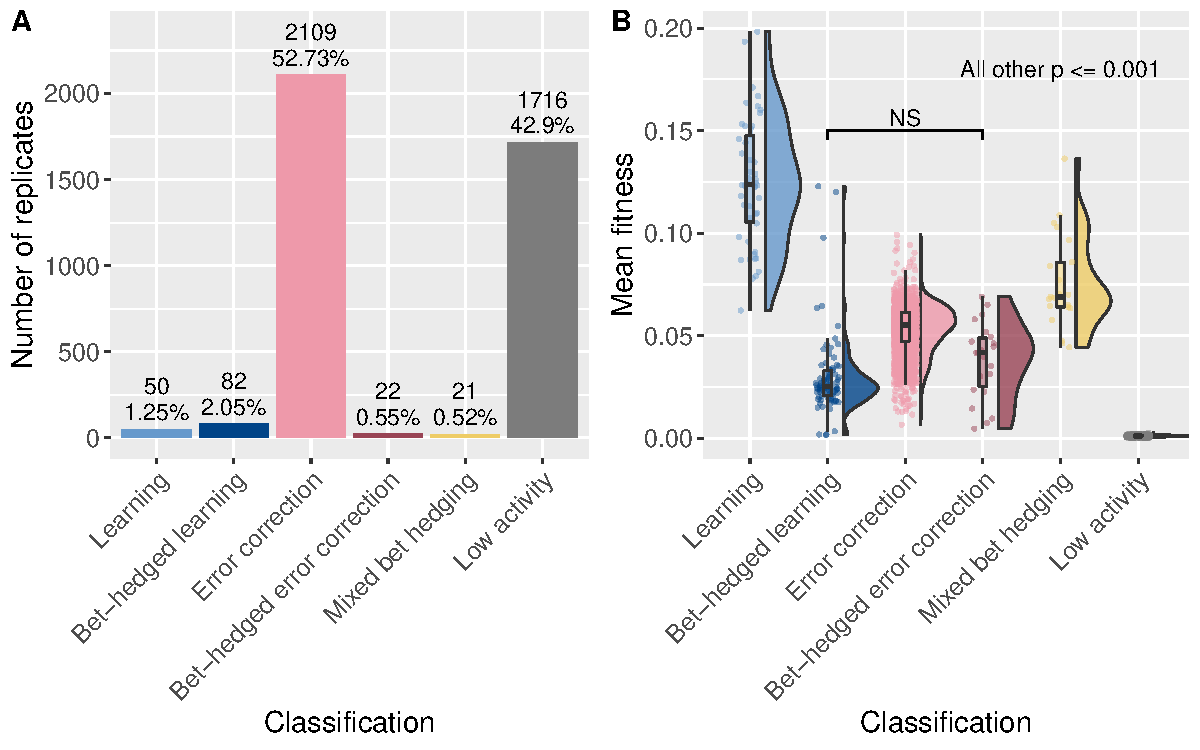
\includegraphics[width=0.9\textwidth]{04_learning_extension/media/initial_reps_stats.pdf}
\end{center}
\caption{ 
Subplot A) Columns show the number of initial replicates whose representative genotype evolved each type of behavior. 
Above each column, the numbers show the number of replicates that evolved that behavior and that count as a percentage of all 4,000 replicates. % (out of 4,000), while the bottom number shows the fraction of replicates.
Subplot B) Raincloud plots show fitness of all 4,000 initial replicates' representative genotypes, grouped by evolved behavior.
All pairwise comparisons are highly significant (p <= 0.001; Pairwise Mann-Whitney with Bonferroni correction) except for the one marked pair (bet-hedged learning and bet-hedged error correction did not have a significant difference).
}\label{fig:initial_reps}
\end{figure}


\subsection{The evolution of learning is exceedingly rare on random paths}
% Initial replicates (Outline)
    % Show categorical outcome figure
    % Learning DOES evolve, but only 1.25% of the time
    % Low activity and error correction account for >95% of replicates
    % Everything else is rare <= 3%
    % We can also look at fitness
        % We see that learning is the most efficient behavior
            % There is some overlap with learning-adjacent behavior (bet-hedged learning / mixed strategy bet-hedging)
        % Otherwise, error correction isn't too far behind learning (sig?)
    % Why is learning so rare here? 
            % It evolved in 8% of replicates in the other chapter
            % And even more than that in Anselmo's work
            % But here, we are evolving on *purely random paths*
            % This removes the first-cue guarantees, and creates a much more challenging bootstrapping problem

As shown in Figure \ref{fig:initial_reps}A, associative learning evolved in only 50 of 4,000 replicates (1.25\%). 
This is considerably lower than the probability of evolving associative learning in previous work, with 8\% of replicates evolving learning in Chapter \ref{chap:learning_case_studies} and up to 14\% in the ``two fixed turns'' environment of \citep{pontesEvolutionaryOriginAssociative2020}.
However, these higher success rates where observed in environments that guaranteed the order of one or more turns at the start of each path. 
In this work we have removed those guarantees entirely; the next step in the path is always uniformly chosen at random among a left turn, right turn, or a step straight ahead.
Thus, we must compare these results to the ``random start'' experiments in 
\citep{pontesEvolutionaryOriginAssociative2020}. 
In their work, zero of 50 replicates evolved learning under such conditions. 
This work therefore marks the first time that associative learning has evolved in Avida without any guarantees about cue ordering. 
It should be mentioned, however, that this work is more lenient with the \texttt{Move Backward} instruction, placing the organism directly back on the path instead of moving them one tile backward and requiring them to reorient on their own, as in \citep{pontesEvolutionaryOriginAssociative2020}.

While learning rarely evolved, error correcting behaviors evolved in the majority (53\%) of replicates. 
Similarly, most of the other replicates (43\%) were classified as ``Low Activity'' as, even at the end of the evolutionary replicate, they failed to correctly identify at least 25 cues in any of 100 trials. 
The remaining replicates evolved bet-hedged behaviors, with bet-hedged learning, bet-hedged error correction, and mixed bet hedging each present in less than 3\% of final evolved populations.

Finally, we see that organisms that perform learning have significantly higher fitness than organisms performing any other strategy (Figure \ref{fig:initial_reps}B, all $p << 0.001$, pairwise Mann Whitney with Bonferroni corrections for multiple comparisons). 
Mixed bet hedging has the next highest fitness, falling between its two constituent parts, learning and error correction. 
Bet-hedged learning and bet-hedged error correction both have lower fitness, on average, than their non-bet hedged counterparts. 
Finally, ``Low activity'' has very low fitness, as expected. 
These fitness values show us that learning was not rare because it was a poor solution to the problem, but rather due to the rugged nature of the underlying fitness landscape.

%\subsection{All replicates see windows of significant potentiation gain}
\subsection{Substantial increases in potentiation are common}

% Substantial increases in potentiation are common
    % We can look at this at two levels: 
        % 1. Exploratory (windows)
        % 2. Targeted (individual steps)
    % At the exploratory level *every* replayed replicate shows significant increase within a single window
        % This varies quite a bit, as we see in the distribution figures
    % At the targeted level, most replayed replicates show significant increase with a single step
        % But not all, we have exactly one non-significant replicate, and a few more are only weakly significant (p <= 0.05)
    % Is this consistent with preexisting replay replicates? 
        % In our work, yes!
        % Other digital studies?
            % Yedid? 
            % Covert?
        % In natural systems...
            % Zach's work... maybe?
            % Meyer paper?
            % C Turner paper? 
            % Jochmusen?
            % Other new papers?

\begin{figure}[h!]
\begin{center}
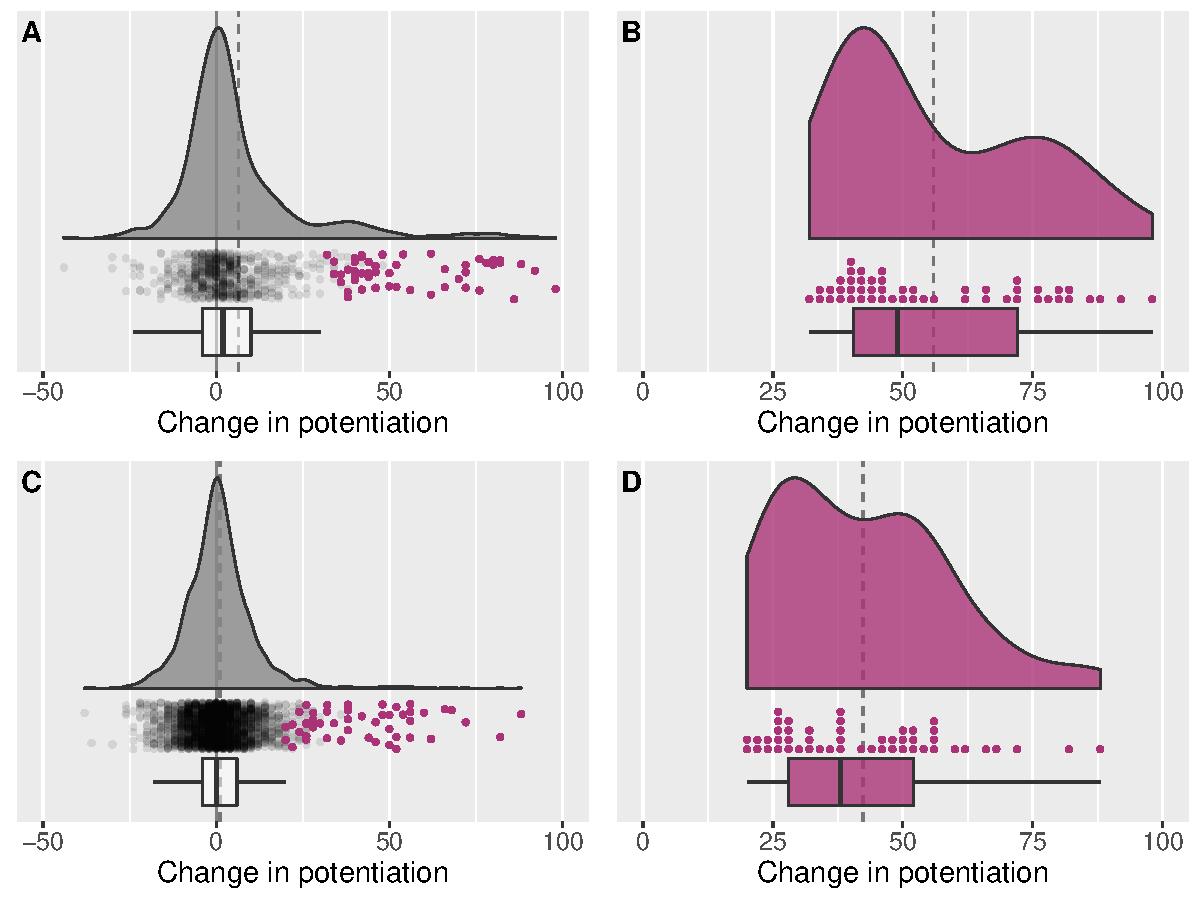
\includegraphics[width=0.9\textwidth]{04_learning_extension/media/replays_dists.pdf}
\end{center}
\caption{ 
Aggregate data for the exploratory replays (A,B) and targeted replays (C,D) of learning replicates. 
Subplots A and C) Raincloud plots showing the distribution of potentiation changes for the cumulative effects across all replayed windows (A) or the individual effects of all replayed lineage steps (C).
The solid vertical line shows zero change and the dashed vertical line shows the mean of the potentiation changes. 
For each of the 50 replicates, a purple point shows the maximum single-window (A) or single-step (C) potentiation increase.
These 50 points are then shown in isolation in (B) and (D).
Subplots B and D)  Raincloud plots showing the distribution of maximum single-window (B) or single-step (D) potentiation changes for each replicate (one point for each of the 50 learning replicates). 
The dashed vertical line shows the mean of these changes. 
}\label{fig:replay_distributions}
\end{figure}

\begin{figure}[h!]
\begin{center}
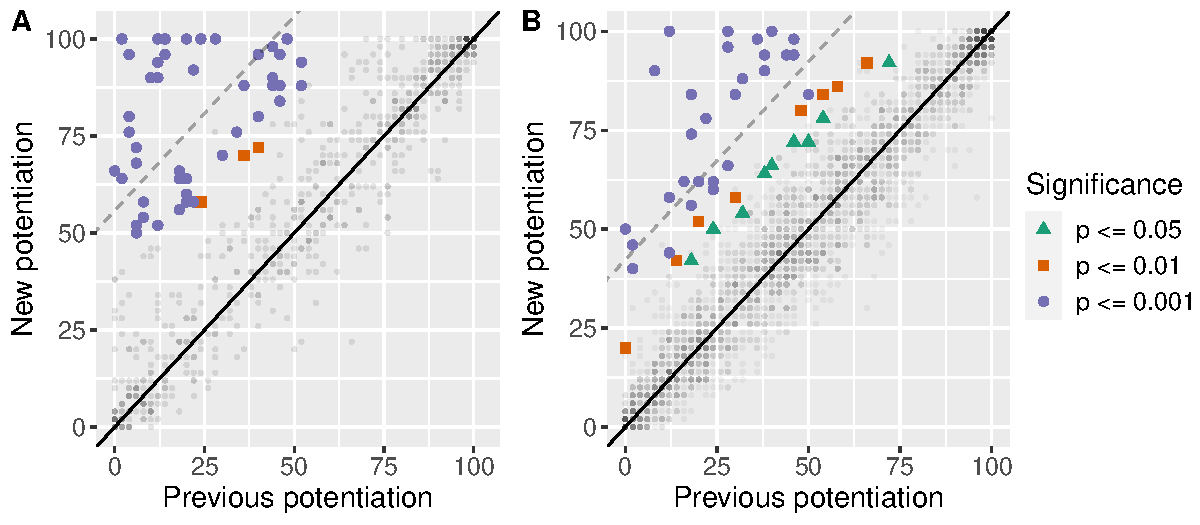
\includegraphics[width=0.9\textwidth]{04_learning_extension/media/replays_stats_legend_on_right.pdf}
\end{center}
\caption{ 
Scatter plot showing the potentiation before and after each exploratory window (Subplot A) or lineage step (Subplot B). 
The color and shape of the 50 main points show significance of the potentiation change (Fisher's exact test).
Semi-transparent points show the rest of the per-window (A, 10\% opacity) or per-step (B, 5\% opacity) potentiation changes. 
The line shows $y=x$, or no potentiation change. 
Potentiation gain is the vertical distance to this line. 
The dashed line shows the maximum potentiation gain of each replicate, averaged across all 50 replicates. 
}\label{fig:replay_stats}
\end{figure}

\begin{figure}[h!]
\begin{center}
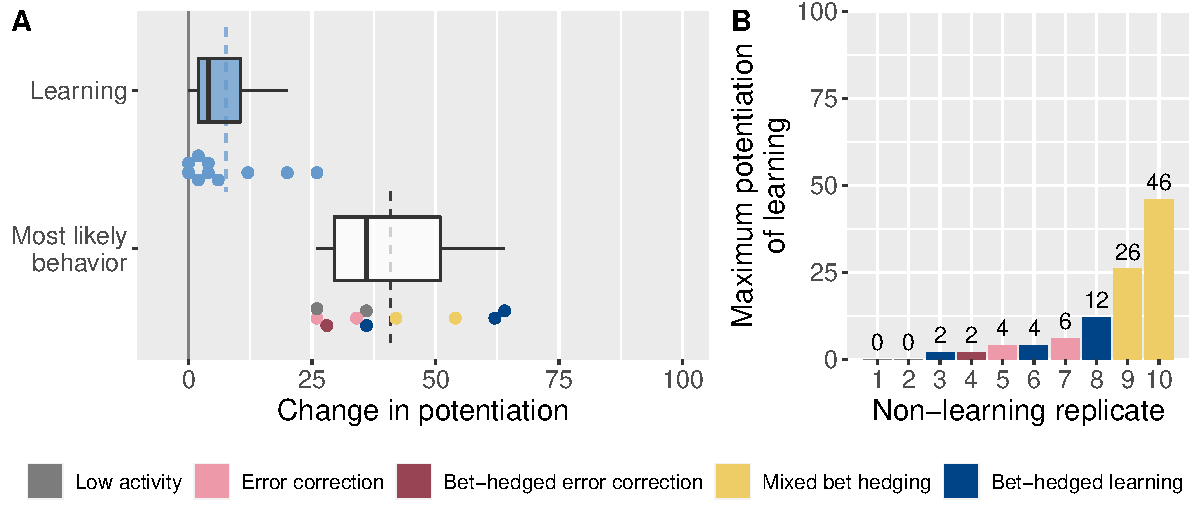
\includegraphics[width=0.9\textwidth]{04_learning_extension/media/non_learning_with_max.pdf}
\end{center}
\caption{ 
Subplot A) Distribution of the maximum per-window change in potentiation for learning (top) and most likely behavior to evolve (bottom) of each of the 10 replayed non-learning replicates.
Colors for the bottom distribution indicate the most likely behavior for each replicate.
Vertical dashed lines show the mean for each group.
Subplot B) The maximum potentiation level of learning observed in each of the 10 non-learning replicates, sorted. 
}\label{fig:non_learning}
\end{figure}

By number of replays conducted, this work is the largest study of potentiation via analytic replay experiments to date. 
Here we detail the key finding of this work: large increases in potentiation are not only possible, but are \textit{common} in this system.
This result is supported at multiple levels, as we detail below. 
For all 50 replicates, figures showing potentiation over time for both exploratory and targeted replays are available in the \hyperref[chap:app_a]{appendix}.

\subsubsection{All replicates have windows of significant potentiation gain}

Exploratory replays show us that, on average, the 50-step windows we replay show little potentiation gain (mean $\approx 6$, median = 2 percentage points) (see Figure \ref{fig:replay_distributions}A).
However, we see that these replays also cover a wide range, from -44 (i.e., 44 percentage points of potentiation \textit{loss)} to $+98$ (i.e., effectively full gain in potentiation in only 50 lineage steps). 

%When we consider the 50 learning replicates, we can also examine the maximum potentiation gain of each replicate (i.e., the potentiation gain of the \textit{potentiating window}).
When we consider these 50 learning replicates, we can also examine the maximum per-window potentiation gain of each replicate.
These maximum gains are highlighted in Figure \ref{fig:replay_distributions}A and shown in isolation in Figure \ref{fig:replay_distributions}B.
When only considering these maximum per-replicate gains, we see a mean gain of approximately $+56$, a median gain of $+49$, and a range of $[+32, +98]$ percentage points.
Figure \ref{fig:replay_stats}A shows all potentiation gains as a combination of their previous and new potentiation values. 
We see that potentiation increases significantly for all 50 learning replicates, even with only 50 replays each ($p \leq 0.01$, Fisher's exact). 
Indeed, 47 of these replicates are highly significant ($p \leq 0.001$). 
Thus we have further evidence that potentiation of learning can increase considerably in a relatively short amount of time. 

%\subsection{Large jumps in potentiation exist in most, but not all, replicates}
% \subsubsection{Large single-step increases in potentiation exist in most, but not all, replicates}
\subsubsection{Significant single-step increases in potentiation exist in all replicates}

While we see these large increases in potentiation over 50-step intervals, we can also look at smaller timescales. 
Indeed, the targeted, single-step replay results tell a similar story. 
Figure \ref{fig:replay_distributions}D shows the potentiation gains at \textit{all} replayed steps.
Here, the mean is approximately $+1$, the median is 0, and the range is $[-38, +88]$ percentage points. 
Thus we see a similar trend to the exploratory replays: the bulk of the distribution residing near zero, but with a short tail in the negative direction and a long tail in the positive direction. 

Focusing on only the maximum potentiating step for each lineage (Figure \ref{fig:replay_distributions}D), we see a mean of approximately $+42$, a median of $+38$, and a range of $[+20, +88]$ percentage points. 
Immediately we see that, in many replicates, a single step in the dominant lineage can account for 50 percentage points of the potentiation of associative learning. 
However, not all replicates see these huge jumps; multiple replicates have a potentiating step of less than 25 percentage points. 
When we examine the individual potentiating steps (Figure \ref{fig:replay_stats}B), we see that all of these changes are significant. 
Of the 50 replicates, 32 were significant at $p \leq 0.001$, nine more at $p \leq 0.01$, and the final nine additional replicates at $p \leq 0.05$. 

\subsubsection{Non-learning replicates see windows of potentiation increase in other behaviors}

We also see evidence of large gains in potentiation of behaviors other than learning. 
Figure \ref{fig:non_learning} details the results of our ten non-learning replicates that were replayed. 
Of these 10 replicates, the single-window potentiation gains for learning were relatively small, with a mean increase of $+7.6$, median of $+4$, and a range of $[0, +26]$ percentage points.
These low values are not surprising, however, as these lineages did not ultimately evolve learning. 
The potentiation for learning was never actualized and eventually lost. 
It should be noted that, even so, a potentiation gain of 26 percentage points over 50 lineage steps is substantial, which is highly significant ($p \leq 0.001$, Fisher's exact). 
Indeed, we see that one of the ten replicates reached a maximum learning potentiation of 46\% at one point in its evolutionary history, though seven replicates never crossed more than a 6\% chance of evolving learning (Figure \ref{fig:non_learning}B).

While the non-learning replicates did not see large increases in the potentiation of learning, they did see large increases in the potentiation of other behaviors. 
Figure \ref{fig:non_learning}A also shows the largest per-window potentiation increase in the most likely behavior at the end of evolution. 
Here we see a mean of $+40.8$, a median of $+36$, and a range of $[+26, +64]$ percentage points.
All of these differences are significant ($p \leq 0.01$, Fisher's exact), and eight of them highly significant ($p \leq 0.001$). 
Thus, the large increases in potentiation that we have observed are \textit{not} limited to the evolution of learning. 
% It should also be noted that two behaviors, error correction and low activity, are limited in their maximum potentiation gain. 
% Since both behaviors have a $>40\%$ chance of evolving from the naive ancestor (Figure \ref{fig:initial_reps}A), they either must first decrease in potentiation, or they are capped at $<60$ percentage points of gain in potentiation, and thus it is unlikely we would witness a 80 percentage point increase like we observed in the some learning replicates. 
Our expectation is that we would observe large single-step potentiation increases for these non-learning behaviors too if we conducted targeted replays on these lineages.
Figures of how potentiation changed over time for all 10 non-learning replicates are available in the \hyperref[chap:app_a]{appendix}. 
%appendix \ref{chap:app_a} (Figure \ref{fig:app_a_non_learning}).

\subsubsection{Comparison to other works}

In addition to a deeper investigation into the underlying patterN associated with historical contingency, the original motivation for this work was to validate the findings of Chapter \ref{chap:learning_case_studies} and provide evidence as to their generality. 
That is, we wanted to test if the large per-window and per-step increases we observed in that work were common or if they were mere flukes. 
Indeed, we can now confirm that both the per-window and single-step potentiation increases from that chapter are common in this particular system. 
The maximum per-step potentiation increases we observed in the previous chapter (range of $[+36, +64]$ percentage points) fall comfortably within the range that we observe here ($[+20, +88]$ percentage points).

% Our one direct comparison -- Blount et al. 2008
% Their jumps were much smaller
It is more difficult to compare these results to other works, however. 
While several works have leveraged replay experiments to study the potentiation of a particular trait or behavior, only one has applied replays to multiple points in a single lineage \citep{blountHistoricalContingencyEvolution2008}.
Blount et al. replayed multiple time points of frozen \textit{E. coli} from the Ara-3 strain to empirically test the potentiation of citrate metabolism. 
The largest jump in potentiation they found was \localapprox $+13.3\%$, shifting from $0/30$ replicates at generation 31,500 to $4/30$ replicates at generation 32,000 %(i.e., \localapprox 13.3 percentage points across 500 generations). 
This is a much smaller jump in potentiation, measured over a much longer period of time compared to our results in this work as the tests were 500 generations apart.

% Why might we be seeing larger increases in potentiation than in natural systems?
% There are a few (possibly confounding) factors:
% 1) The genetic landscape is much less complicated here than in natural organisms. 
% While Avida is much more complicated than many digital evolution systems, and in this particular system we have the possibility for many mutations from any given genotype (e.g., $>9000$ possible one-step mutations from a genome of length 100), this is nearly trivial in comparison to natural organisms. 
% This could mean that while there are many possible evolutionary paths in this system, there are still significantly fewer possibilities than in natural systems, and thus any individual paths is at a higher probability of selection. 
% 2) A lack of behavior-refinement needed in this system -- as discussed in \citep{blountGenomicAnalysisKey2012}, citrate metabolism underwent considerable refinement after it first evolved, and thus mutations to citrate metabolism might be lost to drift more frequently than learning-actualizing mutations in this system. 
% While associative learning in this system can be refined, we use an ``all or nothing'' definition and thus anything classified as learning should be relatively fit. 
% 3) E.coli evolved well over 100 million years ago, which should imply that they have settled into a rather stable region of the fitness landscape...


% The other good comparison -- Jochmusen et al 2016
While not directly pulling from an evolving lineage, \citet{jochumsenEvolutionAntimicrobialPeptide2016a} tested the effects of individual mutations on the evolution of colistin resistance in \textit{Pseudomonas aeruginosa}. 
Via experimental evolution, they found evidence that two individual mutations (\textit{phoQ} and \textit{pmrB}) each potentiated the evolution of colistin resistance at the $16\frac{\mu g}{ml}$ concentration level.
These two mutations each increased the potential to evolve this colistin level from  a $<5\%$ chance to a $>70\%$ chance. 
These results directly align with our results -- that a single mutation can drastically increase the probability of a focal behavior evolving. 

% Other works
% Caroline's work -- Never saw extinction in a replay
% Justin Meyer's work -- They were comparing across strains
% Art Covert's work -- Strong effect of a single deleterious mutation
% Dave Bryson's dissertation -- Strong effects in short term replays
For other works, \citet{turnerReplayingEvolutionTest2015} performed similar analytic replay techniques, but never saw the focal results -- the extinction of the Cit$^{-}$ clade in the Long Term Evolution Experiment -- in any of the replay replicates. 
\citet{meyerRepeatabilityContingencyEvolution2012} replayed combinations of Phage $\lambda$ and \textit{E. coli}. 
While some of their results are striking (e.g., the ``all-or-nothing`` pattern of OmpF receptor targeting across certain treatments), the comparisons were across strains and thus not a direct comparison. 
In prior digital work, \citet{covertiiiExperimentsRoleDeleterious2013} showed that a single deleterious mutation could increase the evolution of a complex behavior in Avida (the EQU logic task) from 13/20 (65\%) to 20/20 (100\%) of evolutionary replicates, providing further evidence of substantial potentiation gain from a single mutation.
Similarly, \citet{brysonEvolutionaryPotentialPopulations2012} showed multiple instances of $\geq 50$ percentage points of increase in short-term (always 10,000 updates) replays of EQU in Avida. 

% Do we want a paragraph summarizing these different results? 
% Most studies you cannot compare
% Those you can are mixed
%   A few have small changes (Blound, Turner)
%   Others match well (Jochmusen, Meyer, Covert III, Bryson)

\subsection{Increases in potentiation are often driven by a single mutation}
% Single mutations often drive increases in potentiation
    % Of our 50 replayed learning replicates, the largest potentiation step occured with only one mutation in 30 replicates
    % Of the 30 other replicates, we see that 14 of them have exactly one significant contributor, which is a standalone mutation

\begin{figure}[h!]
\begin{center}
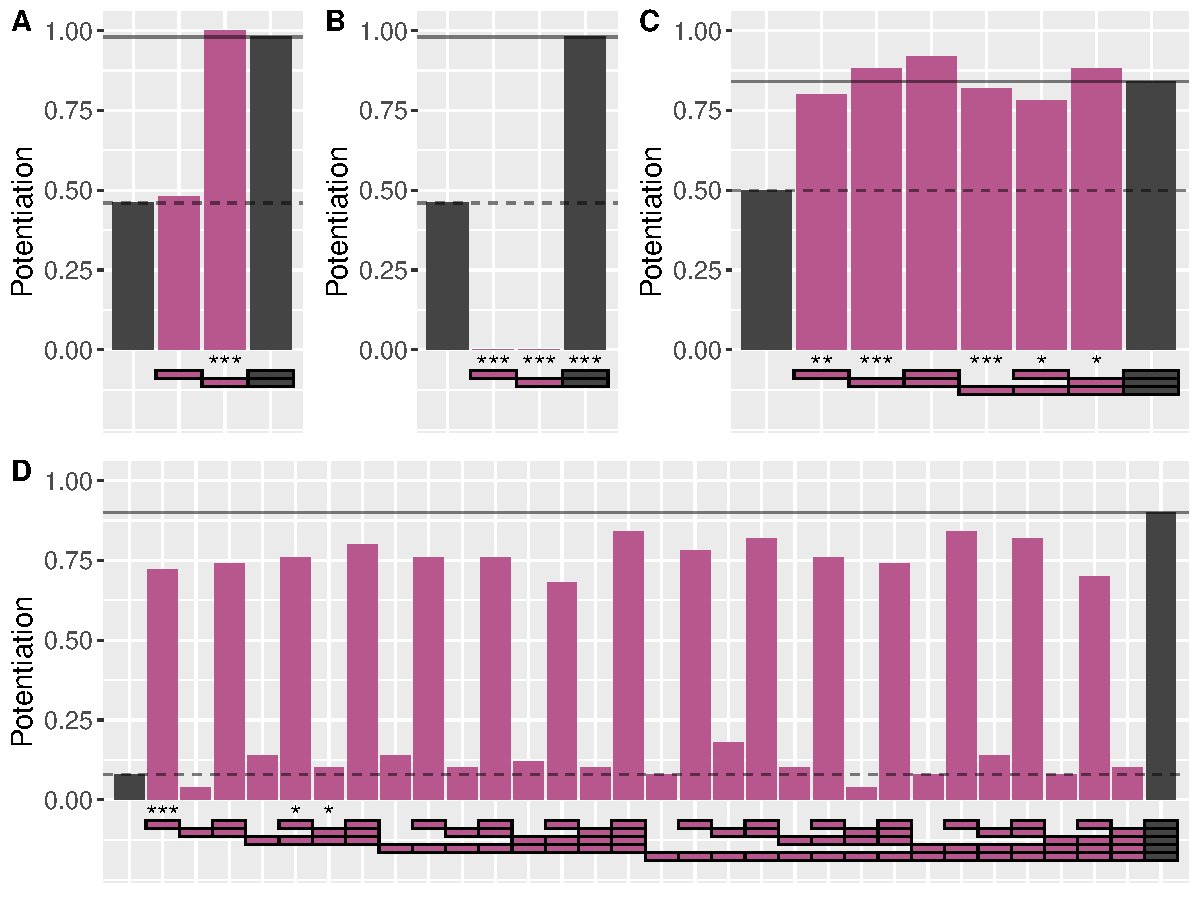
\includegraphics[width=0.9\textwidth]{04_learning_extension/media/mut_splits.pdf}
\end{center}
\caption{ 
Selected results from the mutation split experiment. 
For each subplot, the rightmost column shows the potentiation immediately after the largest potentiating step in that replicate (also shown via solid horizontal line), and the leftmost column shows the potentiation immediately before that step in the lineage (also shown via dashed horizontal line). 
This potentiating step involved $N$ mutations, where $N$ is 2 for subplots A and B, 3 for subplot C, and 5 for subplot D.
There are a total of $2^N$ bars in each subplot, representing the $2^N$ possible combinations of these mutations, as indicated by the small boxes below each bar.
The left bars show potentiation with none of the $N$ mutations presents, the right bars have all $N$ mutations present,
%These two steps are separated by $N$ mutations,
and the middle bars (purple) show the potentiation of every other possible combination of these mutations. 
Significance of each mutation combination in the logistic regression is shown under each column (* for $p \leq 0.05$, ** for $p \leq 0.01$, *** for $p \leq 0.001$). 
%Finally, the small boxes show the presence of individual mutations, with columns increasing in binary order.
In subplots A and D potentiation is driven by just one of the mutations; in B potentiation requires both mutations (which are individually lethal); and in C all three mutations are independently-potentiating. 
}\label{fig:mut_splits}
\end{figure}

For each of the learning lineages, we have identified the potentiating step; that is, the step in the phylogeny that conferred the largest increase in potentiation. 
Since Avida has a per-site rate for substitution mutations, and insertion and deletion mutations that can occur simultaneously, these lineage steps can consist of more than one mutation. 
Even so, 60\% of the potentiating steps (30 of 50) are comprised of only one mutation. 
Of the remaining 20 potentiating steps, 14 steps contained two mutations, three steps contained three mutations, one step contained four mutations, and two steps contained five mutations. 

Of course, the 30 potentiating steps that consisted of a single mutation must be driven by that particular mutation. 
For each of the other 20 potentiating steps (where multiple mutations co-occurred), we ran replay experiments to split the mutations and determined that not all were necessary to increase potentiation. 
Indeed, % of the 20 steps that consisted of more than one mutation, 
in 14 cases we identified exactly one mutation that significantly increased potentiation on its own. 
The two steps involving five-mutation are included here, as a single mutation explained the potentiation gain in both cases. 
Data from an example of potentiation being driven by one of two co-occurring mutations can be seen in Figure \ref{fig:mut_splits}A, and an example of one driving mutation out of five total mutations can be seen in Figure \ref{fig:mut_splits}D. 

As discussed above, other work has shown that single mutations can have a large impact on potentiation. 
This has been shown in colistin resistance in \textit{Pseudomonas aeruginosa} \citep{jochumsenEvolutionAntimicrobialPeptide2016a} and in the evolution of EQU in Avida \citep{covertiiiExperimentsRoleDeleterious2013}.
Thus we have instances where potentiation increases drastically with single mutations in both digital and natural organisms. 
% Conversely, while we see some evidence for the slow accumulation of potentiation (i.e, 50-step windows with significant potentiation gain but no individual mutations within the window that significantly increase potentiation), we have not found evidence of this dynamic in natural systems in the potentiation literature. 


\subsection{Mutation interactions influence potentiation}
% Mutation interactions influence potentiation
    % Of the 6 replicates that did not rely on one single mutation, at least four had interesting interactions among there mutations
    % Two had epistatic interactions -- the individual mutations were lethal, but together they were potentiating
    % One had two mutations additively accounting for the increase in potnetiation
    % One had three independent mutations, where each mutation would have increased potentiation, but the combination did nothing
    % The final two had no significant factors, and thus we cannot classify them


While we are able to confidently say that many replicates saw potentiation increase with a single mutation, we also observed instances where potentiation changes appeared to require interactions across multiple simultaneous mutations, or other unexpected interactions. %, including their interactions, can influence potentiation.
We identified one replicate where two mutations independently increased potentiation, and combined they accounted for the full step's potentiation gain. 
In one of the steps containing three mutations, all three mutations independently increased potentiation significantly, but the combination of mutations did not further increase potentiation (Figure \ref{fig:mut_splits}C). 
In two replicates we see strong sign epistasis; each step consisted of two mutations, and when analyzed independently these mutations proved to be lethal (and thus potentiation is 0), but when the mutations were combined the resulting mutants were not only viable, but potentiated (Figure \ref{fig:mut_splits}B). 
This is akin to the case study of EQU potentiation in \citep{covertiiiExperimentsRoleDeleterious2013}, where two deleterious mutations (one nearly lethal) combined to actualize EQU.
Finally, of the 50 replicates, two were found to have no significant mutation effects, and further replicates would be required to disentangle the effects of the mutations and their interactions.

%\subsection{Potentiating mutations are still undetectable as they occur in an evolving population}
%\subsection{Potentiating mutations are cryptic in evolving populations}
\subsection{No real-time hallmarks of potentiating mutations were evident in an evolving population}

\begin{figure}[h!]
\begin{center}
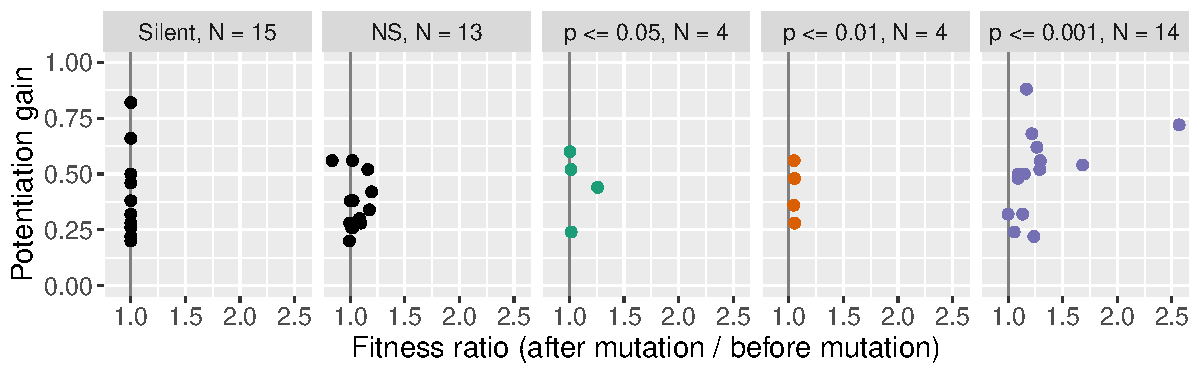
\includegraphics[width=0.9\textwidth]{04_learning_extension/media/fitness_diffs.pdf}
\end{center}
\caption{ 
The fitness effect and potentiation gain of the potentiating step of all 50 learning replicates. 
To calculate fitness, both the potentiation step and the step before it were evaluated on the same set of 100 random seeds. 
We ran a paired Wilcoxon rank-sum test for these two fitness groups for each replicate, and divided and colored the results based on these significance findings. 
Non-significant points are split into those that are truly silent mutations (i.e., zero change in fitness across all 100 trials) and those that are not (fitness values changed, but not significantly). 
The fitness ratio, used for the x-axis, is calculated as the average post-mutation fitness divided by the average pre-mutation fitness. 
The vertical line shows a fitness ratio of one, which indicates no change in the average effect. 
}\label{fig:fitness_diffs}
\end{figure}

As discussed in Chapter \ref{chap:learning_case_studies}, while we can retrospectively identify potentiating mutations, we have yet to find strong indicators of these mutations \textit{during evolution}.
Any such consistent indicators would be invaluable for problem solving with evolutionary computation or other forms of applied evolution. 

Our early hypothesis was that these potentiating mutations are likely to be deleterious, or at least neutral. 
Our reasoning was that if the mutations are beneficial, they would already be likely to be selected and thus they would already be factored into  %expect that their appearance would not drastically alter long-term 
evolutionary potential. 
Of the four case study lineages in Chapter \ref{chap:learning_case_studies}, we saw that one potentiating step was deleterious, two were neutral, and one was beneficial. 

Here, we have refined our methods to compare the potentiating step to the step before it, evaluating both genotypes on the same set of 100 random paths to conduct a pairwise comparison (Figure \ref{fig:fitness_diffs}). 
Using a paired Wilcoxon test, we find that in 28 of 50 lineages the potentiating step did not have a significant effect on realized fitness. 
Indeed, in 15 of these replicates, the two genotypes displayed \textit{exactly} the same behavior -- the mutations were truly silent, while in 13 changes to fitness occurred, but not enough to meaningfully change the distribution.
The truly neutral mutations may be modifying instructions that are executed but do not directly effect the phenotype, or they could be cryptic genetic variation occurring in unexpressed regions of the genotype (Chapter \ref{chap:consequences_of_plasticity}). 
Of the remaining 22 replicates with significant changes to fitness, we find that 21 significantly increase fitness, and only one mutation was significantly deleterious. 
Further, our one deleterious mutation was significant ($p < 0.001$) but not substantial, with less than a 1\% change in fitness. 

The fitness effects of the significantly beneficial mutations varied wildly,  with many conferring small impacts on fitness. 
Two mutations had a greater than 50\% increase in fitness, one of which had a fitness over 250\% of the pre-mutation fitness. 
Thus, we have strong evidence against our hypothesis that potentiating mutations are likely deleterious. 
We observe that potentiating mutations are often neutral or nearly-neutral, though they can also drastically increase fitness. 
%In a genetic space as complicated as Avida's, we now realize that even if a mutation is highly beneficial, there are likely other highly-beneficial mutations, even if they are few, and thus these beneficial mutations are not guaranteed to sweep and thus can affect potentiation.
In a genetic space as complicated as Avida's, even highly-beneficial mutations are not guaranteed to be found, let alone sweep.
Given the number of alternative possibilities, some of which may be highly advantageous themselves, even beneficial mutations can be highly potentiating.
Indeed, even if deleterious mutations would open up new pathways through the genotype space, the low probability of them gaining substantial numbers in the population may eliminate the possibility of them being potentiating.

One final hypothesis for identifying potentiation mutations \textit{as they occur} is to look for mutations that alter the overall behavioral phenotype. 
Of the 50 potentiating lineage steps that we analyzed, we found that 43 of 50 left the underlying behavioral phenotype unchanged. 
Of the seven that did change the phenotype, all were originally error correction behaviors. 
After the potentiating step, five then shifted to a mixed bet hedging strategy -- they still performed error correction on some paths but were capable of learning on others. 
One more replicate evolved learning \textit{with the potentiating step}, likely representing a low probability mutation that was actualized. 
The final behavior-changing mutation shifted the behavior from error correction to bet-hedged error correction. 
While this replicate might represent an interesting case -- the degradation of behavior -- the majority of potentiating mutations did not change the behavior and thus behavior changes are not a reliable indicator of potentiating mutations when they occur. 
%% Discussion
% This section may be divided by subheadings. Discussions should cover the key findings of the study: discuss any prior research related to the subject to place the novelty of the discovery in the appropriate context, discuss the potential shortcomings and limitations on their interpretations, discuss their integration into the current understanding of the problem and how this advances the current views, speculate on the future direction of the research, and freely postulate theories that could be tested in the future.

\section{Discussion}
% Discussion outline
    % Large single-step potentiation gains are common, but not ubiquitous
        % Median > 35%, Mean > 40%
        % Some jumps are as large as 80%
        % However, we also see instances as low as 20%
        % How many are significiant?

    % These potentiating events are overwhelmingly driven by single mutations
        % 30/50 were just one mutation to start with, 14 more seem to be driven by one mutation 

    % Still no metrics to detect potentiating mutations as they occur
        % Fitness effects can be anything
        % Only a few (7/50) change the behavioral phenotype
Here we place the results of this work in a broader evolutionary biology context. 

\subsection{Drastic increases in potentiation are common}

\subsection{Single mutations often drive increases in potentiation}

\subsection{Mutation interactions influence potentiation}

\subsection{Potentiating mutations are still undetectable in an evolving population}

\section{Conclusion}
% Conclusion (outline)
    % This is the first study to look into potentiation in the aggregate
        % How does this relate to other studies? 
            % Confirms ALife 2023 was not a fluke
            % Provides evidence of step-function potentiation (a la Blount 2008)
            % Other papers? 
    % Is this applicable to natural systems? 
        % Not directly!
        % The methods could be employed, but this does not mean that this effect is seen in other digital systems, let alone in natural systems. 
    % Future work
        % Expand to other systems

% General intro - what have we done here?
Here we have conducted a study of potentiation with the largest number of analytic replay experiments to date.
By replaying 50 lineages of digital organisms that evolved associative learning, we have provided further evidence that potentiation can increase suddenly, with strong evidence that a single mutation can result in large increases in potentiation. 
We have also shown that potentiation can increase as a result of the co-occurrence of multiple mutations, with or without epistatic interactions. 
Finally, we were unable to find a signal for these potentiating mutations when they appear -- as such, we are still only able to identify these mutations retrospectively. 

\subsection{Limitations and applicability to other systems}
% This system is clearly digital

% We see similar dynamics in some works in natural systems

% However, some works saw much smaller increases in potentiation
% Factors: 
%   - Simpler genetic landscape
%   - Learning is very likely to stick around
%       - In part because it requires very little refinement to be beneficial

% Using clonal population restarts will create larger jumps in potentiation than population snapshots

%

In both this work and Chapter \ref{chap:learning_case_studies} we primarily investigate the potentiation of one behavior, associative learning, in the Avida digital evolution framework. 
As such, we cannot claim that the potentiation dynamics observed in this work are globally applicable. 
Indeed, we can only claim these results as evidence that large, single-mutation increases in potentiation are \textit{possible}, and that, in certain systems, they might be common. 

While this work is among the first to explore \textit{patterns} in potentiation across many evolved lineages, it is far from the first to explore potentiation dynamics. 
Do the results of other studies match the large increases in potentiation we observed for the evolution of associated learning in Avida? 
In some cases it appears that short spans of evolution, and in fact even single mutations, confer substantial increases in potentiation \citep{jochumsenEvolutionAntimicrobialPeptide2016a, covertiiiExperimentsRoleDeleterious2013}. 
These increases are not universal, as other works have seen maximum increases in potentiation substantially lower than observed here \citep{blountHistoricalContingencyEvolution2008}.
In conducting these comparisons, however, we must consider that the sample sizes for these other works are quite low and that may bias our comparisons.
Additionally, all replay replicates in \citep{blountHistoricalContingencyEvolution2008} evolved for the same number of generations regardless of the starting point, while we ensured that all replay replicates experienced the same number of Avida updates as the original lineage experienced after the sampled genotype appeared. 
We would expect the former scheme to observe substantially lower potentiation in replicates founded from earlier points in the population's history. 
Finally, it is possible that the lineages in these other studies \textit{did} see substantial increases in potentiation, but those particular changes were missed in those experiments. 

% Our mutational neighborhoods are smaller, and thus any given mutation is more likely to occur
If these potentiation dynamics truly differ, what might explain these differences? 
While Avida has a rich and complex genetic architecture compared to many other digital evolution experiments, these digital organisms are still vastly less complex than even the most simple natural bacteria.
An Avida organism in this work, with our original genome length of 100 instructions, has roughly 9,000 possible one-step mutations that can occur. 
With a naive assumption that every nucleotide could mutate to any other nucleotide at every site in the \textit{E. coli} genome (\localapprox 4.6 million base pairs, \citet{blattner1997complete}), we would expect over 13 million one-step substitution mutations alone. 
While this is only a rough estimate, it is clear that the likelihood of a particular mutation appearing is much lower in natural organisms, which can bias the potentiation changes. 
This difference only compounds as we consider the likelihood of multiple necessary mutations arising and fixing.
Therefore, we expect that natural organisms will typically see lower levels of potentiation for equivalent genetic distances from the focal behavior.

% Learning in our system needs little refinement, and also it is a "terminal" behavior
Additionally, there is likely a difference in how the focal behavior arises and is classified. 
We are stringent in our system and only classify a behavior as learning if it is already well-refined, and thus even the first organism in the population to be classified as having evolved learning is likely to have high fitness. 
In natural systems, biologists will often denote a non-trivial trait or behavior as present even if it still requires considerable refinement. 
For example, in the \textit{E. coli} studies in the LTEE, citrate metabolism was not highly advantageous initially, but rather needed considerable refinement before it rose to prominence in the population \citep{blountGenomicAnalysisKey2012}.
Thus, even genotypes capable of weak citrate metabolism may still have low potentiation for maintaining that trait in the longer term, as it may be lost before it is refined. 
Follow-up work to our study should consider analyzing the potentiation of all forms of learning, including bet-hedged learning and mixed bet hedging strategies that combine learning and error correction, to see if potentiation dynamics change. 
Further, learning is a terminal behavior in our system -- the lack of open-endedness dictates that once learning evolves, it is unlikely to be replaced with a more effective survival strategy. 
Combined, these factors may create larger increases in potentiation, and should be dissected in future digital studies. 

% Final, clonal populations vs population snapshots, population sizes
Finally, our system uses small population sizes (3,600 organisms) compared to natural systems (which are often in excess of tens of millions of organisms), and our replay techniques may also bias the changes in potentiation. 
By using a smaller population size, we increase the effect of genetic drift on our population and increase the likelihood that neutral or even deleterious mutations can spread before being purified. 
In fact, by replaying populations via a full clonal population of an genotype from the dominant lineage, we are resetting all population dynamics from the potentiation measurements. 
During normal evolution of a population, not only does a mutation need to occur, but the organism in which it resides also needs to successfully replicate at least once. 
By using clonal populations for our replay experiments, we ensure that every mutation establishes, eliminating possible intermediate potentiation values. 

\subsection{Future work}

% Other analyses?
    % Distance to focal behavior
        % Meaningful distance to focal behavior
    % Did the potentiating mutation exist at the time of actualization

% Expanding beyond Avida and learning
In this chapter we described our deep analysis of the potentiation dynamics behind the evolution of associative learning in Avida. 
First and foremost, future work should investigate potentiation dynamics in a range of other systems. 
Digital systems as simple as bitstring evolution problems could illuminate how the dynamics are affected by factors such as mutation rate and population size. 
Slightly more complicated systems could investigate characteristics of the genetic space such as connectedness, dimensionality, mutational operators, or crossover.
Finally, more wet-lab studies of potentiation across a wider range of environments or in a more varied selection of natural organisms can provide more real-world grounding for these results, though such systems are considerably more labor-intensive. 

% Other potentiation dynamics - anti-potentiating mutations
As we alluded to in Chapter \ref{chap:learning_case_studies}, not only are we interested in identifying mutations that substantially increase potentiation, but we are also interested in the mutations that significantly \textit{decrease} potentiation. 
In this work we replayed ten replicates that did not evolve associative learning, to see how their potentiation dynamics differed from ``successful'' replicates. 
Even within those ten replicates we observed one replicate that reached a height of 46\% potentiation for associative learning. 
Extending this idea, if we have 50 replicates that evolved learning, we might expect 100 replicates to have reached 50\% potentiation but only half of them to have succeeded in that coin flip. 
This conjures the question: do we see large decreases in potentiation similar to the increases observed in this work? 
Are there single mutations that doom a would-be promising lineage to an ``unsuccessful'' fate? 
For example, an immediately beneficial mutation might sweep through a population trapping it on a local optima and preventing it from following a pathway that would lead a population to higher levels of fitness.
Identifying these anti-potentiating mutations in real time could potentially be as valuable as identifying potentiating mutations as they could allow us to slow the evolution of pathogenic or otherwise harmful populations.
While additional studies would be needed to fully delve into these dynamics, early work should dive into this dataset. 
When conducting replay experiments, we are effectively quantifying the potentiation of \textit{each} possible behavior. 
Thus we have non-learning potentiation data, but analyzing this data is outside the scope of this chapter. 

% Improving methods
Finally, additional work is needed to identify techniques that reduce the cost of performing replay experiments. 
This work has taken one step: iterating backward from the appearance of the focal behavior during the exploratory replay phase. 
Additional optimizations could include minimizing the original number of replicates per replayed time step and then running additional replicates for those that seem interesting. 
Finding more efficient ways of searching for potentiating steps is critical. 
We cannot directly perform a binary search for finding the largest potentiating step, as potentiation does not increase monotonically and thus large increases in potentiation can be hidden by decreases in the same window. 
However, there may be variations of binary search that will provide the maximum potentiating step within some margin of error or the maximum \textit{sustained} increase in potentiation. 
In particular, using digital systems to find and verify these ideas might make future \textit{in vitro} experiments more tractable to perform. 

% Conclusion
Overall, these results provide a useful benchmark for any future projects that use replay experiments to study historical contingency. 
As more studies of mutations are conducted, we can refine our ideas about how potentiation changes over the course of a population's history. 
As we progress, we can leverage our understanding of potentiation dynamics to better infer what happened in the evolution of life around us, better prepare for how populations will evolve under climate change, and better leverage evolution to solve technical problems. 
% \documentclass[letterpaper]{article}

% \usepackage{natbib,alifeconf,amsmath,multirow,makecell,hyperref}  %% The order is important
% \usepackage[table]{xcolor}
% \usepackage{textcomp}
% \newcommand{\localapprox}{\raisebox{0.5ex}{\texttildelow}}


% *****************
%  Requirements:
% *****************
%
% - All pages sized consistently at 8.5 x 11 inches (US letter size).
% - PDF length <= 8 pages for full papers, <=2 pages for extended
%    abstracts (not including citations).
% - Abstract length <= 250 words.
% - No visible crop marks.
% - Images at no greater than 300 dpi, scaled at 100%.
% - Embedded open type fonts only.
% - All layers flattened.
% - No attachments.
% - All desired links active in the files.

% Note that the PDF file must not exceed 5 MB if it is to be indexed
% by Google Scholar. Additional information about Google Scholar
% can be found here:
% http://www.google.com/intl/en/scholar/inclusion.html.


% If your system does not generate letter format documents by default,
% you can use the following workflow:
% latex example
% bibtex example
% latex example ; latex example
% dvips -o example.ps -t letterSize example.dvi
% ps2pdf example.ps example.pdf


% For pdflatex users:
% The alifeconf style file loads the "graphicx" package, and
% this may lead some users of pdflatex to experience problems.
% These can be fixed by editing the alifeconf.sty file to specify:
% \usepackage[pdftex]{graphicx}
%   instead of
% \usepackage{graphicx}.
% The PDF output generated by pdflatex should match the required
% specifications and obviously the dvips and ps2pdf steps become
% unnecessary.


% Note:  Some laser printers have a serious problem printing TeX
% output. The use of ps type I fonts should avoid this problem.



%\title{Non-Epistatic Genetic Interactions Potentiate Exploration under Adaptive Momentum}
%\title{Adaptive Momentum Potentiates Evolutionary Exploration}
%\title{Predicting the Unpredictable: Using Replay Experiments to Isolate Changes in Adaptive Potential for Evolving Populations Outside of Equilibrium}
%\title{Predicting the Unpredictable: Using Replay Experiments to Isolate Changes in Evolutionary Potential for Non-equilibrium Populations}
%\title{Predicting the Unpredictable: Replay Experiments can Measure Changes in Evolutionary Potential during Disruptive Events}
%\title{Predicting the Unpredictable: Disentangling Long-Term Evolutionary Dynamics by using Replay Experiments to Measure Changes in Adaptive Potential}
%\title{Predicting the Unpredictable: Using replay experiments to disentangle how particular population dynamics affect evolutionary outcomes}
%\title{Predicting the Unpredictable: Using replay experiments to disentangle how evolutionary outcomes are altered by particular population dynamics}
%\title{Predicting the Unpredictable: Using replay experiments to disentangle how evolutionary outcomes are altered by adaptive momentum}
\chapter{Predicting the unpredictable: Using replay experiments to disentangle how evolutionary outcomes are altered by adaptive momentum}
\label{chap:adaptive_momentum}

\noindent
Authors: Austin J. Ferguson, Charles Ofria, and Clifford Bohm 

\noindent This chapter is adapted from a paper that has been peer-reviewed and accepted to appear in the proceedings of the 2024 Conference on Artificial Life. 

In this work we use the lens of historical contingency and potentiation to provide a new vantage point in understanding the adaptive momentum effect. 
According to the adaptive momentum framework, when a population is in disequilibrium some advantaged organisms can buffer more deleterious mutations than usual. 
This increased buffering increases evolutionary exploration until equilibrium is reestablished. 
Here we replay the evolution of select populations evolving in an idealized environment: a one-dimensional sawtooth function.
At each step we are able to quantify their potential to cross the next deleterious fitness valley. 
We find that populations experiencing disequilibrium, here caused by a selective sweep, see their potential to cross increase drastically with mutations near the leading edge of the sweep. 
Conversely, populations in equilibrium rely purely on chance to cross -- only the last mutations before a valley cross confer an increase in potential. 
Finally, we also performed ``shuffled'' replays to demonstrate that the structure of the population, not just its genetic makeup, is key in increased valley-crossing potential in this system. 

% KEY TERMS: Historical contingency, adaptive momentum, replay experiments, potentiation, disequilibrium, evolutionary dynamics, selective sweeps
%\author{}
%\author{Austin J. Ferguson$^{1,2,3,*}$, Charles Ofria$^{1,2,3}$, Clifford Bohm$^{3,4}$  \\
% \mbox{}\\
%  $^1$Department of Computer Science and Engineering
%  $^2$Program in Ecology, Evolution, and Biology\\
%  $^3$BEACON Center for the Study of Evolution in Action 
%  $^4$Department of Integrative Biology \\
%  Michigan State University, East Lansing, MI 48824 \\
% $^*$fergu358@msu.edu} % email of corresponding author


% For several authors from the same institution use the same number to
% refer to one address.
%
% If the names do not fit well on one line use
%         Author 1, Author 2 ... \\ {\Large\bf Author n} ...\\ ...
%
% If the title and author information do not fit in the area
% allocated, place \setlength\titlebox{<new height>} after the
% \documentclass line where <new height> is 2.25in



% \begin{document}
% \maketitle

% \begin{abstract}
% % Abstract length should not exceed 250 words
% % 210/250 words used
% (250 words max, shorter preferred).
When a new evolutionary dynamic is identified, researchers often struggle to understand its long-term effects on evolutionary outcomes.
Evolutionary prediction is always challenging, as subtle nuances of dynamics can interact in unpredictable ways.
Digital evolution systems, however, provide an empirical alternative to prediction: automated replay experiments can be conducted in large numbers to measure a real distribution of outcomes from a given starting point.
Changes in distributions over time can help us understand the long-term implications of seemingly minor events during evolution.
We apply this technique to ``adaptive momentum'', a new framework that explains how phenomena like selective sweeps can temporarily weaken selection and enhance the likelihood of crossing deleterious fitness valleys.
We show that deleterious mutations along the leading edge of a selective sweep can have an outsized influence on the evolutionary fate of a population.
Indeed, we see that evolutionary potential to cross new deleterious valleys drastically increases during selective sweeps.
Moreover, each valley crossing initiates a new sweep, increasing the potential for further discoveries; this increased potential subsides only once all sweeps have concluded.
While we still have much to learn about both adaptive momentum and the role of history in evolution, this work identifies important evolutionary dynamics at play and hones our tools for further studies.

% \end{abstract}

\section{Introduction}

% Innovations in science and technology periodically create opportunities to conduct experimental studies that were previously relegated to the realm of thought experiments. 
% This shift occurred with Stephen Jay Gould's idea of ``replaying the tape of life'' -- starting evolution over again to see if we would arrive at similar outcomes \citep{gouldWonderfulLifeBurgess1990}. 
% Previous researchers have brought this thought experiment into reality by leveraging microbial populations that can be frozen and then revived \citep{blountContingencyDeterminismEvolution2018} or digital populations that can be saved and loaded at will \citep{fergusonPotentiatingMutationsFacilitate2023}.
% By restarting evolution from different time points in an evolved population's history, researchers have begun to formalize \textit{analytic replay experiments} to test hypotheses on historical contingency.
% %Researchers have begun to leverage these \textit{analytic replay experiments} and the evolutionary counterfactuals they generate to test hypotheses on historical contingency.
% %Researchers have begun to leverage \textit{analytic replay experiments} where populations are restarted from particular time points to generate evolutionary counterfactuals and test hypotheses on historical contingency.
% Below we explore how these techniques can be expanded to develop a deeper understanding of evolutionary dynamics, in this case exploring the concept of ``adaptive momentum''.

% \subsection{Replay Experiments and Evolutionary Prediction}

% Traditional evolutionary biology is often focused on improving our ability to predict evolutionary outcomes or understand why evolutionary history played out the way it did.
% Prediction can be especially difficult in light of complex fitness landscapes with epistatic interactions, meaning that the result of mutational combinations cannot always be known based on individual effects.
% %, where one mutational event can change the impact of others, sometimes even making would-be deleterious mutations into beneficial ones.
% %Given the speed of modern digital evolution systems, however, we are able to shift from trying to simply predict evolution to empirically measuring the range and distribution of possible outcomes.
% Given the speed of digital evolution, however, we do not always need to predict evolutionary trajectories; we can often empirically measure the range and distribution of possible outcomes.
% % Further, by comparing the possible outcomes at different points in evolutionary history, we can determine how particular events influence the likelihood of different outcomes (i.e., historical contingency). 
% % These experiments/techniques allow us to refine our understanding of different dynamics and how they interact. 
% %Armed with not just what evolutionary endpoints were reached, but how particular events (even individual mutations) influenced which outcomes are more or less likely (i.e., historical contingency), we will be able to refine our understanding of different dynamics and how they interact.
% %Armed with not just evolutionary outcomes, but how particular events -- even individual mutations -- influence those outcomes (i.e., historical contingency), we can refine our understanding of different dynamics and how they interact.
% We can even directly measure historical contingency by conducting replay experiments before and after a particular event (such as one or more mutations).% to analyze the change in the distribution of outcomes.

% Thus far, these analytic replay experiments have been employed to study the genetic potentiation of complex traits, such as citrate metabolism in \textit{E. coli} \citep{blountHistoricalContingencyEvolution2008}, novel receptor usage in Phage $\lambda$ \citep{meyerRepeatabilityContingencyEvolution2012}, and associative learning in digital organisms \citep{fergusonPotentiatingMutationsFacilitate2023}.
% %Here we shift the focus from the evolution of a particular target trait and instead apply replay experiments to study fundamental evolutionary phenomena.
% Instead of focusing on the evolution of a particular target trait, here we apply replay experiments to an idealized model system to study fundamental evolutionary phenomena.
% %Instead of replaying the evolution of a particular complex trait, here we shift to a simplified model to use these techniques to better understand fundamental evolutionary phenomena. 

In Chapter \ref{chap:intro} we discussed how researchers are beginning to use analytic replay experiments to quantify how long-term evolutionary outcomes changed over the course of a population's history. 
Indeed, in Chapters \ref{chap:learning_case_studies} and \ref{chap:learning_distributions} we employed these replay techniques to identify key ``potentiating'' mutations in the evolution of associative learning in Avida. 
Here, we use these same replay techniques to understand the ``adaptive momentum'' effect \citep{Bohm2024.04.08.588357}.

Previously, replay experiments have been employed to measure the potentiation of complex traits and behaviors, both in microbial organisms \citep{blountHistoricalContingencyEvolution2008, meyerRepeatabilityContingencyEvolution2012, guptaHostparasiteCoevolutionPromotes2022, jochumsenEvolutionAntimicrobialPeptide2016a} and in digital organisms (Chapters \ref{chap:learning_case_studies} and \ref{chap:learning_distributions}).
Here we instead focus on the potentiation of a significantly simpler task: crossing deleterious fitness valleys in a one-dimensional sawtooth function. 
These fitness valleys require exactly six mutations to cross, which, due to the one-dimensional nature of this system, must be acquired in order. 
Therefore, we already know that any potentiating mutations must be a subset of these six mutations, and thus we are not searching for them as we were in the previous two chapters. 
However, we do not know the \textit{amount} of potentiation conferred by each of these six mutations. 
By comparing these potentiation dynamics of two categories of populations (those in disequilibrium and those in equilibrium), we can directly observe the effect that adaptive momentum has on evolutionary exploration and how these effects change over time. 

\subsection{Adaptive Momentum}

%Here, we use analytic replay experiments to study a newly identified dynamic called ``adaptive momentum'' \citep{Bohm2024.04.08.588357}.
The adaptive momentum framework suggests that periods of disequilibrium resulting from phenomena like selective sweeps and range expansions can enhance genetic exploration \citep{Bohm2024.04.08.588357}. 
We use analytic replay experiments to investigate this effect in selective sweeps.
Consider the appearance of a beneficial mutation in an asexual spatial population. 
If this mutation establishes and is sufficiently strong, it can trigger a selective sweep where the genotypes with the beneficial mutation come to dominate the population.
During the sweep, there will be a boundary between individuals with the beneficial mutation and those without (wild type).
If advantaged individuals along this boundary accrue relatively small deleterious mutations, they may still have a combined fitness benefit over the wild type. 
Thus, individuals along the leading edge of the sweep will have an increased potential to accumulate deleterious mutations that, in turn, increase the potential to explore genetic space and facilitate genetic discovery across fitness valleys. 
Adaptive momentum persists until the wild type is eradicated and equilibrium is reestablished. 
However, if during fixation a new beneficial mutation is discovered, the state of disequilibrium will persist, thus extending the ``momentum window'' (the period of adaptive momentum). 
\footnote{Adaptive momentum describes how disequilibrium during evolution can result in periods of increased mutation buffering. Such disequilibrium can be caused by several conditions, including sweeps, range expansions, and increases in carrying capacity in both spatial and well-mixed populations. The adaptive momentum framework further considers how the increased potential for mutational buffering can also affect large scale evolutionary rates via increased genetic exploration and subsequent genetic discovery.}


%These odds will remain elevated as long as sweeps continue and the population remains in fitness disequilibrium.
%Indeed, any type of fitness disequilibrium will initiate adaptive momentum, including environmental shifts, changes in population capacity, or even extinction events.
%In all cases adaptive momentum can result in beneficial mutations appearing in clustered groups.

In the work presented here, we create an ideal environment for adaptive momentum by using a one-dimensional spatial population evolving on a rising sawtooth fitness function.
%where each peak is higher than the previous, separated by a deleterious valley.
We use replay experiments to measure how the state of the population affects the potential to cross the next fitness valley. 
%We find that the effect of adaptive momentum is clearly visible in this simple system. 
Replay experiments show that %valley crosses are purely reliant on chance in populations not experiencing adaptive momentum. 
%However, 
%under the effect of 
adaptive momentum increases the potential for populations to cross fitness valleys, an effect that diminishes over time.
%Replay experiments show that valley crosses are purely reliant on chance, unless the population is experiencing adaptive momentum. 
%During adaptive momentum, populations see increased potential to cross fitness valleys, though that increase in potential diminishes over time. 
%Replay experiments show that valley crosses are pure chance when adaptive momentum is not in play, while populations experiencing adaptive momentum see increased potential to cross valleys, though that increase does diminish over time. 
%Further, we see that the leading edge of the selective sweep dictates the potential to cross early in the valley, though potential exceeds our expectations later in the valley.

Using simple assumptions about the structure of the leading edge of a selective sweep, we generated a predictive model of the potential for valley crossing during adaptive momentum. 
%This estimation is most accurate for early steps into the fitness valley, but loses accuracy when the leading edge is deeper in the valley and thus more stochastic events may have occurred, resulting in a higher state of disorder, which differs from the assumptions of the model.
While this estimation is highly accurate for early steps into the fitness valley, it loses accuracy when the leading edge is deeper in the valley. 
%This deviation from the predictive model is likely the result of historical contingency.
The time required for a population to reach deeper mutations in the fitness valley is likely also increasing the number of stochastic events that cause differences from the assumptions of the model. 
%The time required for a population to reach deeper mutations in the fitness valley increases the accumulation of stochastic events that increase its differences with the assumptions of the model. 
%This deviation from the predictive model is likely the result of accumulated stochastic events that have occurred in the path to reach deeper mutations in the fitness valley, resulting in a higher state of disorder and more differences with the assumptions of the model.
Finally, by shuffling organism positions in our population snapshots we can disrupt population structure.
This shuffled analysis allowed us to verify that the organization of the population, not just its genetic composition, is vital to valley-crossing potential. 
Overall, this work refines the framework proposed by adaptive momentum while advancing the methodology of analytic replay experiments as a tool for studying historical contingency, exposing sections of both that are ripe for further study. 




% \section{Introduction}

% Innovations in science and technology periodically create opportunities to conduct experimental studies that were previously relegated to the realm of thought experiments. 
% This shift occurred with Stephen Jay Gould's idea of ``replaying the tape of life'' -- starting evolution over again to see if we would arrive at similar outcomes \citep{gouldWonderfulLifeBurgess1990}. 
% Previous researchers have brought this thought experiment into reality by leveraging microbial populations that can be frozen and then revived or digital populations that can be re-instantiated at will.
% Researchers have begun to leverage these \textit{analytic replay experiments} and the evolutionary counterfactuals they generate to test hypotheses on historical contingency \citep{blountContingencyDeterminismEvolution2018}.
% Below we explore how these techniques can be expanded to develop a deeper understanding of evolutionary dynamics, in this case exploring the concept of ``adaptive momentum''.

% \subsection{Replay Experiments and Evolutionary Prediction}

% Thus far, analytic replay experiments have been employed to study the genetic potentiation of complex traits, such as citrate metabolism in \textit{E. coli} \citep{blountHistoricalContingencyEvolution2008}, novel receptor usage in Phage $\lambda$ \citep{meyerRepeatabilityContingencyEvolution2012}, and associative learning in digital organisms \citep{fergusonPotentiatingMutationsFacilitate2023} 
% (See \cite{blountContingencyDeterminismEvolution2018} for a review).
% Here we shift the focus from the evolution of a particular target trait and instead apply replay experiments to study fundamental evolutionary phenomena.

% Traditional evolutionary biology is often focused on improving our ability to predict evolutionary outcomes, or at least understand why evolutionary history played out the way it did.
% Prediction can be especially difficult in light of complex fitness landscapes with epistatic interactions, where one mutational event can change the impact of others, sometimes even making would-be deleterious mutations into beneficial ones.
% Given the speed of modern digital evolution systems, however, we are able to shift from trying to simply predict evolution to empirically measuring the range and distribution of possible outcomes.
% Armed with not just what evolutionary endpoints were reached, but how particular events (even individual mutations) influenced which outcomes are more or less likely (i.e., historical contingency), we will be able to refine our understanding of different dynamics and how they interact.

% \subsection{Adaptive Momentum}

% %Here, we use analytic replay experiments to study a newly identified dynamic called ``adaptive momentum'' \citep{Bohm2024.04.08.588357}.
% The adaptive momentum framework suggests that periods of disequilibrium resulting from phenomena like selective sweeps and range expansions can enhance genetic exploration \citep{Bohm2024.04.08.588357}. 
% We use analytic replay experiments to analyze this effect in selective sweeps.
% Consider the appearance of a beneficial mutation in an asexual spatial population. 
% If this mutation establishes and is sufficiently strong, it can trigger a selective sweep, a disequilibrium state, where the genotypes with the beneficial mutation come to dominate the population.
% During the sweep, there will be a boundary between individuals with the beneficial mutation and those without (wild type).
% If advantaged individuals along this boundary suffer relatively small deleterious mutations, they may still have a combined fitness benefit over the wild type. 
% The individuals along the leading edge of the sweep will have an increased potential to accumulate deleterious mutations that, in turn, increase the potential to explore genetic space, facilitating genetic discovery across fitness valleys. 
% Adaptive momentum persists until the wild type is eradicated. 
% However, if during fixation a new beneficial mutation is discovered, this will extend the ``momentum window'' (the period of adaptive momentum). 
% \footnote{In a most general sense, adaptive momentum describes how any disequilibrium conditions that arise during evolution will result in a period of increased mutation buffering. Adaptive momentum applies to several conditions, including sweeps, range expansions, and increases in carrying capacity in spatial and well-mixed populations. The adaptive momentum framework further considers how the increased potential for mutational buffering can also affect large scale evolutionary rates via changes to increased genetic exploration and subsequent genetic discovery.}


% %These odds will remain elevated as long as sweeps continue and the population remains in fitness disequilibrium.
% %Indeed, any type of fitness disequilibrium will initiate adaptive momentum, including environmental shifts, changes in population capacity, or even extinction events.
% %In all cases adaptive momentum can result in beneficial mutations appearing in clustered groups.

% In the work presented here, we create an ideal environment for adaptive momentum by using a one-dimensional spatial population evolving on a rising sawtooth fitness function.
% %where each peak is higher than the previous, separated by a deleterious valley.
% We use replay experiments to measure how the state of the population results in different potential to cross the next fitness valley. 
% %We find that the effect of adaptive momentum is clearly visible in this simple system. 
% Replay experiments show that %valley crosses are purely reliant on chance in populations not experiencing adaptive momentum. 
% %However, 
% under the effect of adaptive momentum, populations see an increased potential to cross fitness valleys that diminishes over time.
% %Replay experiments show that valley crosses are purely reliant on chance, unless the population is experiencing adaptive momentum. 
% %During adaptive momentum, populations see increased potential to cross fitness valleys, though that increase in potential diminishes over time. 
% %Replay experiments show that valley crosses are pure chance when adaptive momentum is not in play, while populations experiencing adaptive momentum see increased potential to cross valleys, though that increase does diminish over time. 
% %Further, we see that the leading edge of the selective sweep dictates the potential to cross early in the valley, though potential exceeds our expectations later in the valley.

% Using simple assumptions about the structure of the leading edge of a selective sweep, we generated a predictive model of the potential for valley crossing during adaptive momentum. 
% %This estimation is most accurate for early steps into the fitness valley, but loses accuracy when the leading edge is deeper in the valley and thus more stochastic events may have occurred, resulting in a higher state of disorder, which differs from the assumptions of the model.
% While this estimation is highly accurate for early steps into the fitness valley, it loses accuracy when the leading edge is deeper in the valley. 
% This deviation from the predictive model is likely the result of accumulated stochastic events that have occurred in the path to reach deeper mutations in the fitness valley, resulting in a higher state of disorder and more differences with the assumptions of the model.
% Finally, by shuffling organism positions in our population snapshots we can disrupt population structure.
% This shuffled analysis allowed us to verify that the organization of the population, not just its genetic composition, is vital to crossing potential. 
% Overall, this work refines the framework proposed by adaptive momentum while advancing the methodology of analytic replay experiments as a tool for studying historical contingency, exposing sections of both that are ripe for further study. 



\section{Methods}
% Here we describe the system used in this paper and detail the experiments conducted. 

\subsection{Evolution system}
% We used a minimal agent-based digital evolution model where each organism consists of a single integer genome, where fitness is determined as the expinentiation of the result of a sawtooth function based on genome value ($x$).
% To calculate fitness we first generate a score using a ``sawtooth'' function, similar to the one used by [CITE preprint], to create a landscape where local optima are separated by deleterious valleys.  
% Our sawtooth function (\(s\)) is defined as follows: 
% \[
% s(x) = kx - (k+d)(x\ \text{mod}\ w)
% \]
In order to isolate the adaptive momentum effect and keep computational costs feasible, we used a minimal agent-based evolution model where each organism's genome consists of a single integer, with value $x$. 
Fitness is based in a repeated ``sawtooth'' function, similar to the one used in \citep{Bohm2024.04.08.588357}, to create a landscape with regular fitness peaks separated by valleys. 
Each organism is assigned a quality score ($s(x)$), and then that score exponentiated to determine fitness ($f(x)=10^{s(x)}$). 
Score is calculated using the sawtooth function:

% \[
% s(x) = \frac{g}{w}x - (\frac{g}{w}+d)(x\ \text{mod}\ w)
% \]
\[
s(x) = \frac{x - (x~\text{mod}~w)}{w}G - (x~\text{mod}~w)D
\]

\noindent
where $G$ is the gain per peak, $D$ is the decrease per step into the valley, and $w$ is the valley width (number of mutational steps from one peak to the next). 
Effectively, the score function calculates the quality of the highest peak achieved and subtracts the cost of the current mutational step into the valley. 
%We used values of \(k = \frac{1}{6}\), \(a = w = 6\), and \(d = 0.05\).
We used $G=1.0$, $D=0.05$, and $w=6$.
This means that peaks appear every six steps; in this case at $x=6$, $x=12$, $x=18$, and so forth.
We refer to these peaks by their height, so those three peaks would be \(p_{1}\), \(p_{2}\), and \(p_{3}\), respectively.
We refer to the steps between peaks by the prior peak and an offset (\textit{e.g.}, $x=17$ is $p_{2} + 5$, the last step before $p_{3}$).
Figure \ref{fig-sawtooth} illustrates this sawtooth function and the relevant peaks.

Crossing a valley increases an organism's fitness by a factor of 10, and each step into the valley reduces fitness by \localapprox 12\%, relative to the previous peak. %regardless of which peak the organism was on.
We selected these drastic fitness differences to clearly demonstrate the effect.% rather than be representative of typical biological systems. 
%That being said, 
While this degree of selective benefit may be rare in biological systems, cases such as antibiotic resistance can show fitness increases of this magnitude \citep{gullbergSelectionResistantBacteria2011}.
%We stress that the degree of selective advantage modeled here may not represent typical biological systems.

\begin{figure}[h!]
\begin{center}
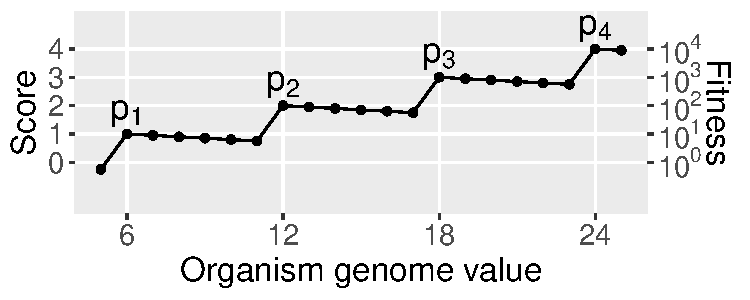
\includegraphics[width=0.75\textwidth]{05_adaptive_momentum/media/sawtooth_conceptual_figure.pdf}
\caption{
    The sawtooth function used in this work, with the four peaks mentioned in this work labeled.
    Score, $s(x)$, and fitness are both shown, with fitness being $10^{s(x)}$.
    %The function and parameters are available in methods. 
}
\label{fig-sawtooth}
\end{center}
\end{figure}

We evolved populations of 512 organisms in a one-dimensional spatial population -- a single line of organisms -- that did not wrap. 
This structure maximizes fixation times and makes selective sweeps easy to track, as they could only move left or right.
The population evolved via discrete, non-overlapping generations. 
%Each new generation of organisms was determined using spatial roulette (i.e., fitness-proportional) selection.%, where roulette selection was performed between the organism and its neighbors (for a maximum of three organisms per selection event). 
To fill positions in the next generation, we performed rounds of spatial roulette selection, each involving three organisms: the organism in that position in the previous generation and its two immediate neighbors (unless the organism is on the edge, in which case the roulette is between only two organisms). 
We then copied the selected individual to produce the offspring, with a $0.0125$ chance to mutate; mutations either increment or decrement the offspring's genome value by one. 
Selective sweeps are thus limited to advancing one position in the population per generation, limiting the growth rate and therefore the fixation time of a beneficial mutation. 
%When an organism is mutated, its integer value is incremented or decremented by one, and we used a mutation of rate of 0.0125 per reproduction event. 

\subsection{Experiment design}

We conducted this work in three stages: 
1) we validated that our model demonstrates adaptive momentum; 
2) we ran ``benchmarking'' data to create an expectation of how potentiation changes during a momentum window; 
and 3) we conducted analytic replay experiments to observe changes in potentiation in evolved lineages. 
Here we outline these experiments in more detail. 

\subsubsection{Experiment I: Model Validation}

%First, we wanted to ensure that our model allowed for valley crossing events, but for those events to be incredibly rare on their own. 
%To accomplish this, we ran 500,000 evolutionary replicates, where each replicate started with 512 organisms at $p_{2}$. 
%These replicates ran for 10,000 generations, much longer than the rest of our experiments, and we tracked the number of generations it took for the populations to cross the valley. 
%Some replicates crossed more than one valley, in which case we recorded the time since the previous crossing. 

%Additionally, we wanted to verify that disequilibrium is what drives the adaptive momentum effect. 

%The goal for our initial experiment was 
To ensure that our model could produce the adaptive momentum effect, 
%To do so, 
we replicated the primary experiment from \citep{Bohm2024.04.08.588357} comparing crossing times in populations starting from equilibrium versus those starting during the disequilibrium of a previous selective sweep. %were affected by the equilibrium state of a population.
We ran 500,000 evolutionary replicates, where each replicate started with 512 organisms at $p_{1}$ and ran for 5,000 generations. 
%, much longer than the rest of our experiments. 
%In the replicates where $p_{2}$ was discovered within in the first 5000 generations, we recorded the number of generations it took to discover $p_{2}$. 
In replicates where $p_{2}$ was discovered, we recorded the generation of discovery and extended the run duration for another 5,000 generations beyond the point of discovery. 
If $p_{3}$ was discovered before time ran out, we recorded this time as well. % to determine if and when $p_{3}$ was discovered. %In replicates that also discovered $p_{3}$, we recorded the number of generations between the discovery of $p_{2}$ and $p_{3}$ if that number was not greater than 5000. 
This methodology produced two time distributions: time to first crossing and time between first and second crossing, both capped at 5,000 generations.
%the first crossing time relative to the start time and the second crossing time relative to the first crossing time.

\subsubsection{Experiment II: Benchmarking}

%Adaptive momentum theory posits that organisms along the leading edge of a selective sweep experience reduced selection, and thus we expected valley crosses to be propelled by the leading edge. 
The adaptive momentum framework posits that populations in disequilibrium experience an increased rate of adaptation. % as long as the disequilibrium persists. 
In spatial populations experiencing a selective sweep, the disequilibrium should manifest near the leading edge of the sweep. 
Specifically, adaptive momentum allows deleterious mutations to accumulate within the advantaged subpopulation along the leading edge. 
This temporarily expanded mutant cloud increases genetic exploration, accounting for an observed increase in the rate of adaptation. 

\begin{figure}[h!]
\begin{center}
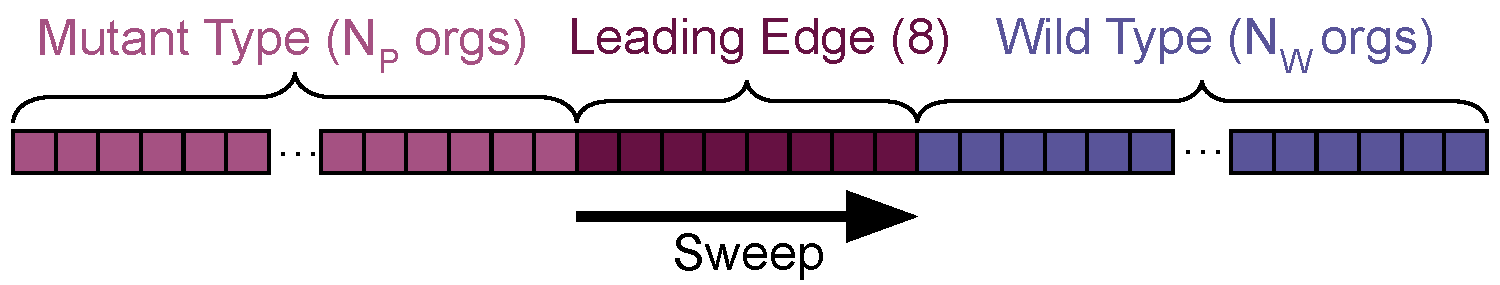
\includegraphics[width=0.85\textwidth]{05_adaptive_momentum/media/sweep_figure.pdf}
\caption{
    Starting layout for experiment II populations, with three clearly-defined sections: $N_P$ ``post-sweep'' mutant organisms at peak $p_{2}$ (left), $N_W$ ``wild type'' organisms at peak $p_{1}$ (right), and 8 ``leading edge'' organisms at a treatment-specific position in the valley past $p_{2}$ (middle).
}
\label{fig-experiment2}
\end{center}
\end{figure}

%We now explain how we apply potentiation to explore these claims.
We created idealized scenarios to study the dynamics of adaptive momentum as they unfold.
Each population had organisms on $p_{2}$ sweeping across organisms on $p_{1}$, with a well-defined leading edge (Fig. \ref{fig-experiment2}).
% of the sweep that are experiencing adaptive momentum.
%  and were experiencing high levels of purifying selection
% and were being swept away
Experimental treatments used all combinations of how far into the next fitness valley the leading edge started (from $x=p_{2}$ to $x=p_{2}+5$), and how far the sweep had progressed across the population (from $N_P=0$, at the beginning of a sweep, to $N_P=504$ at the end.)
%While the leading edge always consisted of eight organisms, its start ranged from position 0 (the beginning of a sweep with no post-sweep organisms) to 504 (the very end of a sweep with no wild-type left), with steps of eight.
%At each position, we tested the six sawtooth values that define a peak and the following valley, from $p_{2}$ to $p_{2} + 5$. 
%The leading edge was always initialized with eight organisms to ensure the post-sweep organisms did not immediately purify the leading edge.
We ran each replicate for $768-N_P$ total generations; the reduced number for larger $N_P$ was used to make the comparison fair, subtracting off the minimum time it could have taken to establish $N_P$ post-sweep organisms.
%, we assumed that if a leading edge is at position $n$ in the population, $n$ updates have already occurred. 
%For example, the replicates with an initial leading edge position of 256 only saw $768 - 256 = 512$ generations of evolution. 
For each condition, we measured how often replicates crossed the next valley to reach $p_{3}$.

We recorded the number of replicates that successfully crossed to $p_{3}$ in each treatment. 
This measurement provided an expectation of a population's potential to cross the valley \textit{based only on the initial state of the leading edge}.
Additionally, we also ran ``shuffled'' controls under otherwise identical conditions, but where we removed population structure (and thus the notion of a leading edge) by randomly shuffling the organisms before each evolutionary replicate.
%The shuffled benchmarks allowed us to evaluate if the population composition was sufficient to account for the results or if the spatial organization of the initialized population, consisting of a leading edge separating the purified post-sweep section from the wild type section, was also important.

\subsubsection{Experiment III: Analytic replays of evolved lineages}

Finally, we focused on the treatment from Experiment II that represented the start of a selective sweep; that is, no post-sweep organisms ($N_P=0$) and a leading edge that just made it to $p_{2}$. %peak 2 ($x=p_{2}$).
We ran 500 replicates under these conditions,
%initialized with the first eight organisms at $p_{2}$ and the rest at $p_{1}$, representing a population at the beginning of a selective sweep shortly after the discovery of a beneficial mutation.
%Again, these replicates evolved for 768 generations. 
saving snapshots at each generation, allowing us to perfectly recreate the population at any time point. 
We randomly selected 10 replicates that failed to reach $p_{3}$, 10 random replicates that did reach $p_{3}$ (but not further), and all four replicates that crossed two valleys to reach $p_{4}$.
For each of these 24 replicates, we performed 1000 analytic replays at every fourth generation, restarting evolution from a given time point with different random seeds to investigate the role of chance in determining \textit{the distribution of potential evolutionary outcomes} \citep{blountContingencyDeterminismEvolution2018}.
Next, we selected one representative sample from each of the three categories to study at high resolution, replaying 10,000 replicates from every generation. 

Using these replays, we recorded the probability that a replicate would cross the valley to $p_{3}$ or $p_{4}$ at each time point. 
These data allow us to calculate how the crossing probabilities changed over time. 
We also ran 10,000 equilibrium replicates and replayed representative replicates in the same manner. 
%This allows us to see how these probabilities changed over time, allowing us to see what generations were key for crossing -- or failing to cross -- that valley. 
%In addition, we recorded the same data for crossing a second valley (to $p_{4}$) in the same manner. 
Finally, just as in the shuffle benchmarking experiment, we performed ``shuffled'' replays on disequilibrium replicates that crossed a single valley.
Specifically, we shuffled the population before starting each replay to measure the role of the population's spatial organization in crossing potential. 

%[TODO - stats?]

\subsection{Data and software availability}
All code, analyses, summarized data, and figures not included in this work are available in the supplemental material \citep{austin_ferguson_2024_11507982}.
The model was built using the Modular Agent Based Evolver version 2.0 (MABE2) (\url{https://github.com/mercere99/MABE2}). 
All analyses and plots were generated using the R statistical computing language version 4.1.2 \citep{r_core_team_r_v4} and the ggplot2 \citep{R-ggplot2}, dplyr \citep{wickhamDplyrGrammarData2022}, HMisc \citep{harrelljrHmiscHarrellMiscellaneous2020}, tidyr \citep{wickhamTidyrTidyMessy2022} packages. %, and khroma \citep{frerebeauKhromaColourSchemes2023} packages. 








% \section{Methods}
% % Here we describe the system used in this paper and detail the experiments conducted. 

% \subsection{Evolution system}
% % We used a minimal agent-based digital evolution model where each organism consists of a single integer genome, where fitness is determined as the expinentiation of the result of a sawtooth function based on genome value ($x$).
% % To calculate fitness we first generate a score using a ``sawtooth'' function, similar to the one used by [CITE preprint], to create a landscape where local optima are separated by deleterious valleys.  
% % Our sawtooth function (\(s\)) is defined as follows: 
% % \[
% % s(x) = kx - (k+d)(x\ \text{mod}\ w)
% % \]

% We used a minimal agent-based evolution model where each organism's genome consists of a single integer, with value $x$. 
% Fitness is based in a repeated ``sawtooth'' function, similar to the one used in \citep{Bohm2024.04.08.588357}, to create a landscape with regular fitness peaks separated by valleys. 
% Each organism is assigned a quality score ($s(x)$), and then that score exponentiated to determine fitness ($f(x)=10^{s(x)}$). Score is calculated using the sawtooth function:

% % \[
% % s(x) = \frac{g}{w}x - (\frac{g}{w}+d)(x\ \text{mod}\ w)
% % \]
% \[
% s(x) = \frac{x - (x~\text{mod}~w)}{w}G - (x~\text{mod}~w)D
% \]

% \noindent
% where $G$ is the gain per peak, $D$ is the decrease per step into the valley, and $w$ is the valley width (number of steps from one peak to the next). 
% Effectively, the score function calculates the quality of the highest peak achieved and subtracts the cost of the current mutational step into the valley. 
% %We used values of \(k = \frac{1}{6}\), \(a = w = 6\), and \(d = 0.05\).
% We used values of $G=1.0$, $D=0.05$, and $w=6$.
% This means that we have peaks appear every six steps; in this case at $x=6$, $x=12$, $x=18$, and so forth.
% We refer to these peaks by their height, so those three peaks would be \(p_{1}\), \(p_{2}\), and \(p_{3}\), respectively.
% We refer to the steps between peaks by the prior peak and an offset (e.g., $x=17$ is $p_{2} + 5$; the last step before $p_{3}$).
% Figure \ref{fig-sawtooth} illustrates this sawtooth function and the relevant peaks.

% Crossing a valley increases an organism's fitness by a factor of 10, and each step into the valley reduces fitness by \localapprox 10\%, regardless of which peak the organism was on.
% We selected these drastic fitness differences to clearly demonstrate the effect rather than be representative of typical biological systems. 
% That being said, while this degree of selective benefit may be rare in biological systems, cases such as antibiotic resistance can show fitness increases of this magnitude \citep{gullbergSelectionResistantBacteria2011}.
% %We stress that the degree of selective advantage modeled here may not represent typical biological systems.

% \begin{figure}[h!]
% \begin{center}
% 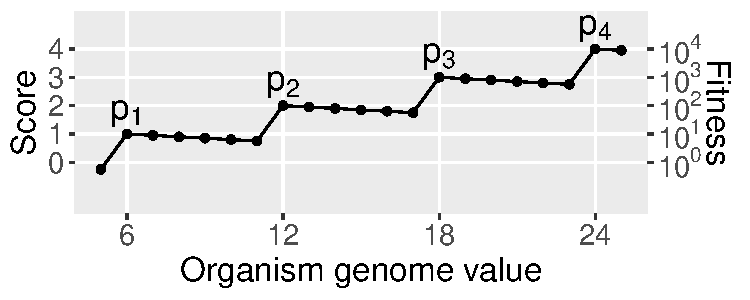
\includegraphics[width=0.75\textwidth]{05_adaptive_momentum/media/sawtooth_conceptual_figure.pdf}
% \caption{
%     The sawtooth function used in this work, with the four peaks mentioned in this work labeled.
%     Score, $s(x)$, and fitness are both shown, with fitness being $10^{s(x)}$.
%     %The function and parameters are available in methods. 
% }
% \label{fig-sawtooth}
% \end{center}
% \end{figure}

% We evolved populations of 512 organisms organized in a one-dimensional spatial population -- a single line of organisms -- that did not wrap. 
% This structure maximizes fixation times and makes selective sweeps easy to track, as they could only move left or right.
% The population evolved via discrete, non-overlapping generations. 
% %Each new generation of organisms was determined using spatial roulette (i.e., fitness-proportional) selection.%, where roulette selection was performed between the organism and its neighbors (for a maximum of three organisms per selection event). 
% To fill a position in the next generation, a round of spatial roulette selection was performed involving three organisms: the organism in that position in the previous generation and its two immediate neighbors (unless the organism is on the edge, in which case the roulette is between only two organisms). 
% The selected individual is then copied to produce an offspring. 
% This copy has a $0.0125$ chance to mutate, which will either increment or decrement the offspring's genome value by one. 
% Selective sweeps are thus limited to advancing one position in the population per generation, limiting the growth rate and therefore the fixation time of a beneficial mutation. 
% %When an organism is mutated, its integer value is incremented or decremented by one, and we used a mutation of rate of 0.0125 per reproduction event. 

% \subsection{Experiment design}

% We conducted this work in three stages: 
% 1) we validated that our model demonstrates adaptive momentum; 
% 2) we ran ``benchmarking'' data to create an expectation of how potentiation changes during a momentum window; 
% and 3) we conducted analytic replay experiments to observe changes in potentiation in the evolved lineages. 
% Here we outline these experiments in more detail. 

% \subsubsection{Experiment I: Model Validation}

% %First, we wanted to ensure that our model allowed for valley crossing events, but for those events to be incredibly rare on their own. 
% %To accomplish this, we ran 500,000 evolutionary replicates, where each replicate started with 512 organisms at $p_{2}$. 
% %These replicates ran for 10,000 generations, much longer than the rest of our experiments, and we tracked the number of generations it took for the populations to cross the valley. 
% %Some replicates crossed more than one valley, in which case we recorded the time since the previous crossing. 

% %Additionally, we wanted to verify that disequilibrium is what drives the adaptive momentum effect. 

% The goal for our initial experiment was to ensure that our model could replicate the adaptive momentum effect. 
% To do so, we replicated the primary experiment from \citep{Bohm2024.04.08.588357} to test whether crossing times were affected by the equilibrium state of a population.
% We ran 500,000 evolutionary replicates, where each replicate started with 512 organisms at $p_{1}$ and ran for 5,000 generations. 
% %, much longer than the rest of our experiments. 
% %In the replicates where $p_{2}$ was discovered within in the first 5000 generations, we recorded the number of generations it took to discover $p_{2}$. 
% In replicates where $p_{2}$ was discovered, we recorded the generation of discovery and extended the run duration for another 5,000 generations beyond the point of discovery. 
% If $p_{3}$ was discovered before time ran out, we recorded this time as well. % to determine if and when $p_{3}$ was discovered. %In replicates that also discovered $p_{3}$, we recorded the number of generations between the discovery of $p_{2}$ and $p_{3}$ if that number was not greater than 5000. 
% This methodology produced two time distributions: time to first crossing and time between first and second crossing, both capped at 5,000 generations.
% %the first crossing time relative to the start time and the second crossing time relative to the first crossing time.

% \subsubsection{Experiment II: Benchmarking}

% %Adaptive momentum theory posits that organisms along the leading edge of a selective sweep experience reduced selection, and thus we expected valley crosses to be propelled by the leading edge. 
% The adaptive momentum framework posits that populations in disequilibrium experience an increased rate of adaptation. % as long as the disequilibrium persists. 
% In spatial populations experiencing a selective sweep, the disequilibrium should manifest near the leading edge of the sweep. 
% Specifically, adaptive momentum allows deleterious mutations to accumulate within the advantaged subpopulation along the leading edge. 
% This temporarily expanded mutant cloud increases genetic exploration, accounting for an observed increase in the rate of adaptation. 

% \begin{figure}[h!]
% \begin{center}
% 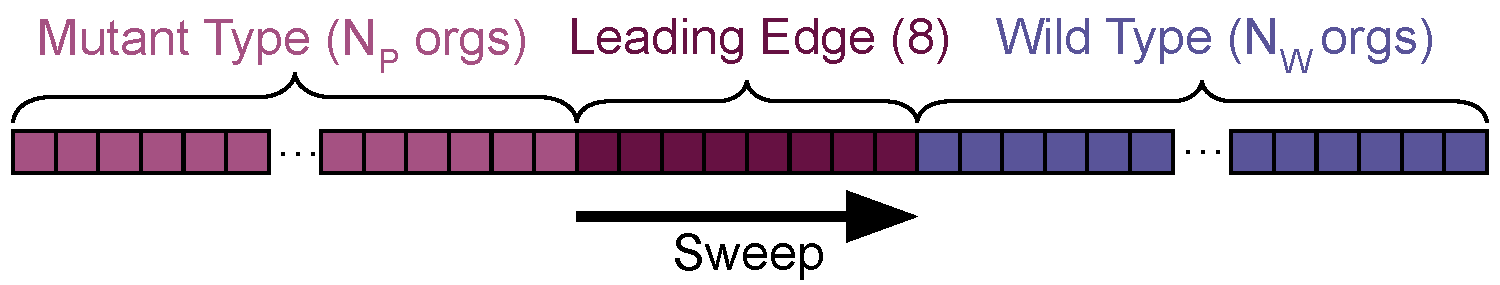
\includegraphics[width=0.85\textwidth]{05_adaptive_momentum/media/sweep_figure.pdf}
% \caption{
%     Starting layout for experiment II populations, with three clearly-defined sections: $N_P$ ``post-sweep'' mutant organisms at peak $p_{2}$ (left), $N_W$ ``wild type'' organisms at peak $p_{1}$ (right), and 8 ``leading edge'' organisms at a treatment-specific position in the valley past $p_{2}$ (middle).
% }
% \label{fig-experiment2}
% \end{center}
% \end{figure}

% %We now explain how we apply potentiation to explore these claims.
% We created idealized scenarios to study the dynamics of adaptive momentum as they unfold.
% Each population had organisms on $p_{2}$ sweeping across organisms on $p_{1}$, with a well-defined leading edge (Fig. \ref{fig-experiment2}).
% % of the sweep that are experiencing adaptive momentum.
% %  and were experiencing high levels of purifying selection
% % and were being swept away
% Experimental treatments used all combinations of how far into the next fitness valley the leading edge started (from $x=p_{2}$ to $x=p_{2}+5$), and how far the sweep had progressed across the population (from $N_P=0$, at the beginning of a sweep, to $N_P=504$ at the end.)
% %While the leading edge always consisted of eight organisms, its start ranged from position 0 (the beginning of a sweep with no post-sweep organisms) to 504 (the very end of a sweep with no wild-type left), with steps of eight.
% %At each position, we tested the six sawtooth values that define a peak and the following valley, from $p_{2}$ to $p_{2} + 5$. 
% %The leading edge was always initialized with eight organisms to ensure the post-sweep organisms did not immediately purify the leading edge.
% We ran each replicate for $768-N_P$ total generations; the reduced number for larger $N_P$ was used to make the comparison fair, subtracting off the minimum time it could take to establish $N_P$ post-sweep organisms.
% %, we assumed that if a leading edge is at position $n$ in the population, $n$ updates have already occurred. 
% %For example, the replicates with an initial leading edge position of 256 only saw $768 - 256 = 512$ generations of evolution. 
% For each condition, we measured how often replicates crossed the next valley to reach $p_{3}$.

% We recorded the number of replicates that successfully crossed to $p_{3}$ in each treatment. 
% This measurement provided an expectation of a population's potential to cross the valley \textit{based only on the initial state of the leading edge}.
% Additionally, we also ran ``shuffled'' controls under otherwise identical conditions, but where we removed population structure (and thus the notion of a leading edge) by randomly shuffling the organisms before each evolutionary replicate.
% %The shuffled benchmarks allowed us to evaluate if the population composition was sufficient to account for the results or if the spatial organization of the initialized population, consisting of a leading edge separating the purified post-sweep section from the wild type section, was also important.

% \subsubsection{Experiment III: Analytic replays of evolved lineages}

% Finally, we focused on the treatment from Experiment II that represented the start of a selective sweep; that is, no post-sweep organisms ($N_P=0$) and a leading edge that just made it to $p_{2}$. %peak 2 ($x=p_{2}$).
% We ran 500 replicates under these conditions,
% %initialized with the first eight organisms at $p_{2}$ and the rest at $p_{1}$, representing a population at the beginning of a selective sweep shortly after the discovery of a beneficial mutation.
% %Again, these replicates evolved for 768 generations. 
% saving snapshots at each generation, allowing us to perfectly recreate the population at any time point. 
% We randomly selected 10 replicates that failed to reach $p_{3}$, 10 random replicates that did reach $p_{3}$ (but not further), and all four replicates that crossed two valleys to reach $p_{4}$.
% For each of these 24 replicates, we performed 1000 analytic replays at every fourth generation, restarting evolution from a given time point with different random seeds to investigate the role of chance in determining \textit{the distribution of potential evolutionary outcomes} \citep{blountContingencyDeterminismEvolution2018}.
% Next, we selected one representative sample from each of the three categories to study at a higher resolution, replaying every generation for 10,000 replicates each. 

% Using these replays, we recorded the probability that a replicate would cross the valley to $p_{3}$ or $p_{4}$ at each of these time points. 
% These data allow us to calculate when and how the crossing probabilities changed over time. 
% We also ran 10,000 equilibrium replicates and replayed representative replicates in the same manner. 
% %This allows us to see how these probabilities changed over time, allowing us to see what generations were key for crossing -- or failing to cross -- that valley. 
% %In addition, we recorded the same data for crossing a second valley (to $p_{4}$) in the same manner. 
% Finally, just as in the shuffle benchmarking experiment, we performed ``shuffled'' replays on disequilibrium replicates that crossed a single valley.
% Specifically, we shuffled the population before starting each replay to determine the role of the population's spatial organization in crossing potential. 

% %[TODO - stats?]

% \subsection{Data and software availability}
% All code, analyses, summarized data, and figures not included in this work are available in the supplemental material \citep{austin_ferguson_2024_11507982}.
% The model was built using the Modular Agent Based Evolver version 2.0 (MABE2) (\url{https://github.com/mercere99/MABE2}). 
% All analyses and plots were generated using the R statistical computing language version 4.1.2 \citep{r_core_team_r_v4} and the ggplot2 \citep{R-ggplot2}, dplyr \citep{wickhamDplyrGrammarData2022}, HMisc \citep{harrelljrHmiscHarrellMiscellaneous2020}, tidyr \citep{wickhamTidyrTidyMessy2022} packages. %, and khroma \citep{frerebeauKhromaColourSchemes2023} packages. 

\section{Results}
%Below we describe the results in the same order the experiments were described, first validating the adaptive momentum effect, then moving onto benchmarking and replay experiment results.  

\begin{figure*}[h!]
\begin{center}
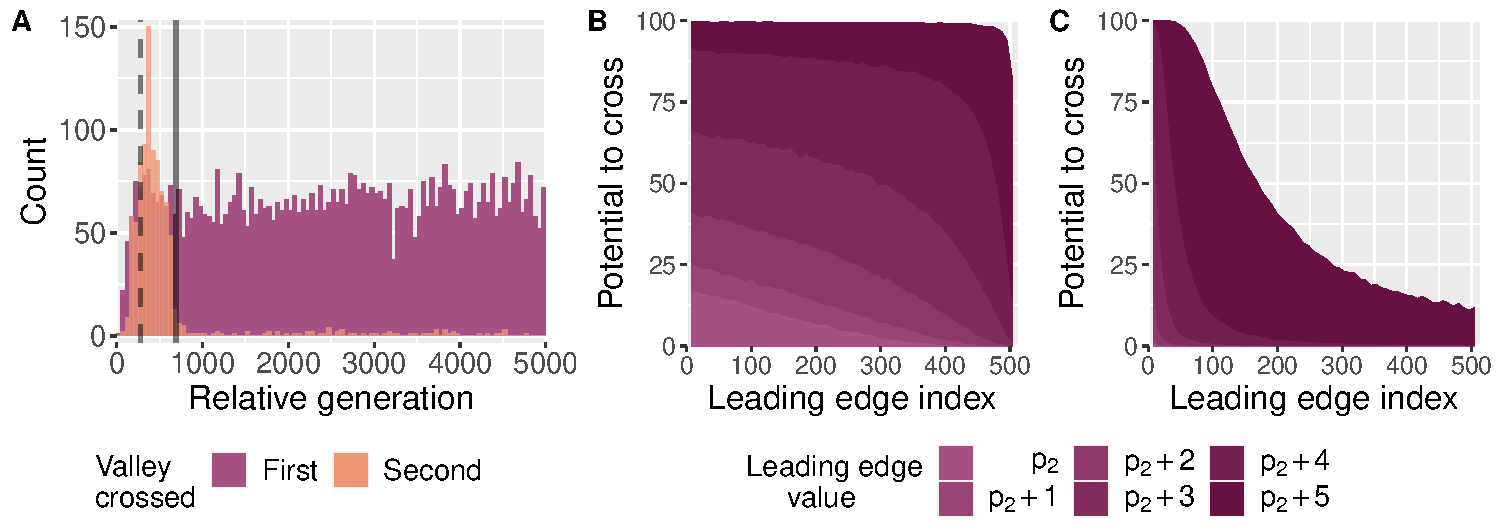
\includegraphics[width=\textwidth]{05_adaptive_momentum/media/combined_plots_full_split.pdf}
\caption{
    (A)
    Distribution of the number of generations required to cross valleys in the validation experiment. 
    Relative generations refer to the elapsed time (in generations) for the first cross (purple), and from the first cross to the second cross (orange). 
    %The solid and dashed horizontal lines show the expected count of first and second crosses per bar, respectively, for the expected uniform distribution. 
    The dashed and solid vertical lines show minimum and maximum fixation times, respectively. 
    (B) 
    Benchmarking data showing the potential of a leading edge to cross a valley, with a range of leading edge starting positions and values (see Fig. \ref{fig-experiment2}). 
    Each point represents 10,000 replicates.
    (C)
    Shuffled benchmarking data. Each replicate is shuffled prior to evolution, otherwise identical to center plot.
}
\label{fig-combined-plots}
\end{center}
\end{figure*}

\subsection{Validation of adaptive momentum effect}

First, we measured the time it took for replicates starting from a full population of $p_{2}$ to cross the valley to $p_{3}$ and, when relevant, from $p_{3}$ to $p_{4}$.
Figure \ref{fig-combined-plots}A
shows the timing distributions of populations that crossed the first valley over the first 5,000 generations (purple) as well as the timing distributions of second crossings that occur within 5,000 generations of a first (orange). 
We see that the time of first crossing appear uniformly distributed across the 5,000 generations, while the second crosses are strongly skewed toward shorter time periods. 
Indeed, of 500,000 replicates, 6,485 crossed the first valley within 5,000 generations (\localapprox 1.3\%) with a mean cross time of \localapprox 2,569 generations and a median of 2,602 generations. 
Based on these values, we would expect roughly 84 replicates to cross twice ($6,485 \times 1.3\%$, or 0.0169\% of all 500,000 replicates), but instead we see 902 replicates (\localapprox 0.18\%) cross the second valley, a much higher rate than expected if the probabilities of first and second crossing were equal.
In addition to a higher than expected rate of crossing, the mean cross time between first and second crossings is \localapprox 579 generations and the median cross time is 401 generations, substantially lower than the first crossing times. 
Finally, when we consider only those second crossing times that occurred more than 1000 generations after a first crossing, we find that the rate of these second crossings is similar to the first crossing rate (\localapprox 1.23\%).
These results comport with the framework of adaptive momentum. 
They show that an initial beneficial discovery can quickly lead to additional discoveries (during the fixation period), but if the second discovery does not happen before equilibrium is reestablished, the rate of valley crossing is better predicted by the first valley crossing times. 


% Indeed, of 500,000 replicates, 12,793 crossed at least once (\localapprox 2.6\%) with a mean cross time of \localapprox 4,995 generations and a median of 4,951 generations. 
% We would expect that only 338 replicates to cross twice (2.6\% squared), but instead we see 1,734 replicates cross at least two valleys (\localapprox 0.35\% of total, or \localapprox 13.6\% of those that crossed once). 
% For the second crossings, we see a mean cross time of 646 generations and a median cross time of 396 generations. 
% Indeed, while not shown in Figure \ref{fig-crosses-from-scratch}, we see 200 replicates cross at least three valleys, 26 replicates cross at least four valleys, and six replicates cross five valleys; of these higher-order crossings, the median time to cross was always less than 420 generations. 
% These findings, where an initial beneficial discovery can quickly lead to additional discoveries, supports the initial adaptive momentum theory. 

% \begin{figure}[h!]
% \begin{center}
% 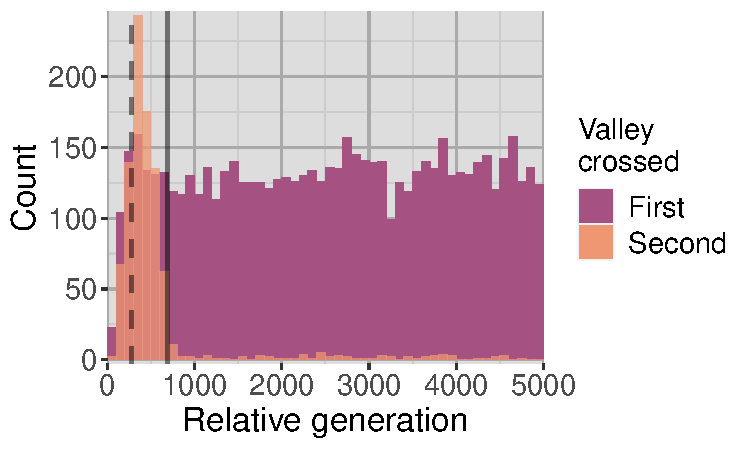
\includegraphics[width=0.45\textwidth]{media/first_two_crosses_overlayed_fair_comparison_with_fixation.pdf}
% \caption{
%     Distribution of the number of updates required to cross valleys in the validation experiment. 
%     Relative updates refer to the number of elapsed generations for the first cross, and the number of generations since the first cross for the second cross. 
%     %The solid and dashed horizontal lines show the expected count of first and second crosses per bar, respectively, for the expected uniform distribution. 
%     The dashed and solid vertical lines show the minimum and maximum fixation times, respectively. 
% }
% \label{fig-crosses-from-scratch}
% \end{center}
% \end{figure}





%Further, we tested the role of disequilibrium in these discoveries by comparing the evolution of populations seeded with eight organisms on $p_{2}$ and the rest on $p_{1}$ (disequilibrium treatment) against whole populations of $p_{2}$ (control). 
%We found that 1,751 of 10,000 disequilibrium replicates crossed the first valley (\localapprox 17.5\%), while only 23 of 10,000 control replicates crossed (\localapprox 0.2\%). 
%This difference is highly significant ($p < 10^{-15}$, Fisher's exact test).
%This further supports the claim that adaptive momentum relies on disequilibrium in the population, and shows that we can start artificially start an adaptive momentum window in this system by creating this disequilibrium. 

\subsection{Empirical benchmarks}

%After confirming that disequilibrium can facilitate valley crosses, we next tested idealized populations to benchmark the effect on valley crossing of two components of this disequilibrium: the position of the leading edge, and the genotypes of the organisms comprising that leading edge.
The empirical benchmark data (Fig. \ref{fig-combined-plots}B) illustrate how the initial state of the population affects the potential to cross valleys.
%In particular the ratio of the population initiated on $p_2$ (mutant type), versus $p_1$ (wild type) and the value of the individuals on the leading edge,
As expected, steps further into the valley increase the probability of crossing, regardless of where the leading edge is. 
On the other hand, the probability of crossing decreases as the ratio of $p_2$ organisms (mutant type) increases relative to $p_1$ organisms (wild type) -- as the selective sweep progresses, fewer opportunities remain for additional mutations to accumulate. 
While the potential to cross varies considerably with the type of organisms in the leading edge, these data clearly show that all conditions describing early sweep conditions (\textit{i.e.}, having a leading edge and a significant ratio of the remaining population on $p_1$) %having any leading edge 
substantially increase the probability of crossing the valley compared to populations that are close to reaching equilibrium on $p_2$. 

%The benchmarks with a leading edge at index 0 see slightly lower rates of crossing, as they only have one organism at the given value while every other point has 8 organ
%We typically ran these benchmarking populations with a leading edge of eight organisms of the same type to remove the possibility of genetic drift immediately destroying the leading edge. 
%This drift accounts for the drop in crosses at index 0, the one instance where the leading edge consisted of only a single organism. 
%Finally, being one step away from crossing the valley ($p_2$ + 5) effectively guarantees a cross, as eight organisms at that value are almost certain to accumulate the one needed mutation unless the selective sweep is almost over. 
%Overall, these data match our expectations. 
We use these results to provide a baseline prediction for the analytic replay experiments. 

% \begin{figure}[h!]
% \begin{center}
% 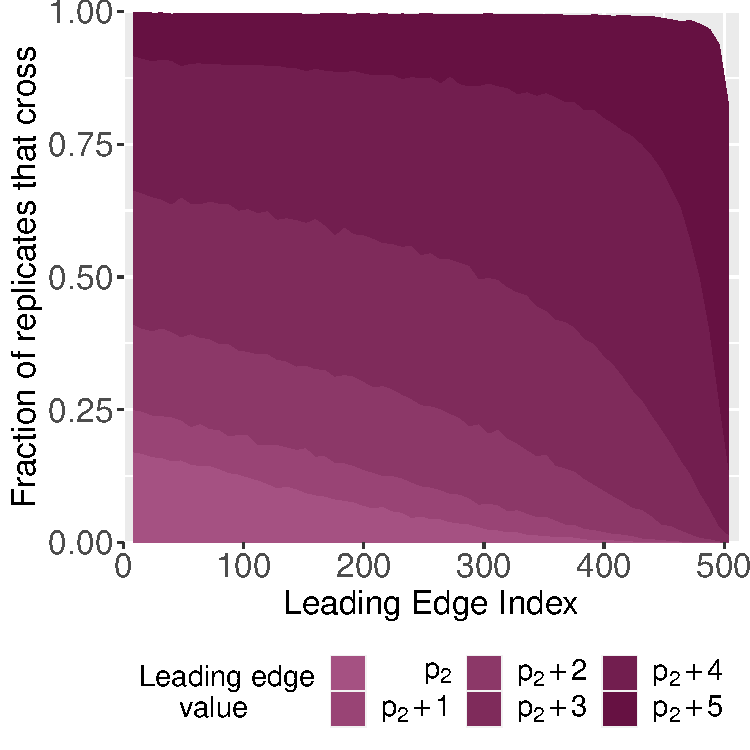
\includegraphics[width=0.45\textwidth]{media/benchmarking_area.pdf}
% \caption{
%     Benchmarking data showing the potential of a leading edge to induce a valley cross, with a range of leading edge values and starting positions. 
%     The leading edge always consists of eight organisms of that value. 
%     Each point represents 10,000 replicates. 
% }
% \label{fig-benchmarking}
% \end{center}
% \end{figure}

\subsection{Analytic replay experiments}
Of our 500 initial replicates to find candidates for replay experiments, four replicates (0.8\%) crossed two valleys in the allotted time, 83 crossed exactly one valley (16.6\%), and the remaining 413 did not cross any valleys (82.6\%). 
%We ran coarse-grained replays for 10 randomly-sampled no-cross replicates, 10 random single-cross replicates, and all four double-cross replicates.
We randomly-sampled 10 no-cross replicates, 10 single-cross replicates, and took all four double-cross replicates to run coarse-grained replays.
%We ran coarse-grained analytic replay experiments for all four replicates that crossed twice and for 10 randomly-sampled replicates of each of the two other categories. 
%For each of these 24 replicates, we replayed at every fourth generation, with 1,000 replicates per time point. 
All plots are available in the supplement \citep{austin_ferguson_2024_11507982}. 

From these coarse-grained replays, we selected one representative replicate from each category to re-run, conducting 10,000 replay trials at \textit{every} time point to give a fine-grained view. 
%We show the replay results in two formats. 
%The first showing the potential of crossing the next valley over time and the second as Muller plots showing the underlying population structure that beget that potentiation. 
For each replayed replicate, we show the potential of crossing the next valley over time, paired with a Muller plot \citep{mullerGeneticAspectsSex1932} of the initial replicate that was replayed. 
Figures \ref{fig-replay-single-cross}, \ref{fig-replay-double-cross}, and \ref{fig-replay-no-cross} show the single-cross, double-cross, and no-cross replicates, respectively. 
%In each plot, the replay results are overlaid atop the benchmarking data, which has been adjusted such that the leading edge index aligns with the actual leading edge at that generation of the population.
In each plot, the replay results are overlaid on an image generated from the benchmark data. 
%To generate the background image, we treat the benchmark data as a lookup function and use the current position of the leading edge of the replay result to look up the potentiation predicted by the benchmark data. 
To generate the background image, we treat the benchmark data as a lookup function.
When we start a replay replicate, we initialize the population using the snapshot from the target generation of the initial replicate. 
These snapshots show that the leading edge does not perfectly advance one position every generation; there are many generations where the leading edge either fails to advance or is pushed back one position by the wild type organisms.
%As we see in our population snapshots, the leading edge does not actually advance one position every generation, the leading often fails to advance, and occasionally the wild-type organisms replicate over the leading edge, pushing it back one step. 
To make this comparison fair, we find the leading edge in that particular snapshot and then look up the corresponding expectation values from the benchmark data. 
%Thus, the background image shows in ``real time'' potentiation of the replay at each generation.
This adjustment ensures that we are comparing against the correct benchmark data regardless of the motion of the leading edge. 
%Thus, the background image adjusts 

Overall, the potentiation observed in all three replicates closely match the benchmark expectations. 
The potentiation occasionally increases or decreases suddenly; tracing these changes to the Muller plots typically shows that these events correlate to the gain or loss of a mutation at (or near) the leading edge at that time. 
For example, the two temporary peaks in potential in Figure \ref{fig-replay-single-cross}, at roughly generations 250 and 375, can be directly traced to the leading edge temporarily dipping to $p_{2} + 4$.
%When the leading edge mutates further into the fitness valley, the potentiation increases dramatically. 
%Each of the three replicates 
The potentiation at any particular step in the valley decreases over time, as the selective sweep progresses and the adaptive momentum window closes.
Figure \ref{fig-replay-no-cross} shows that, while the replicate had substantial potentiation at times (briefly above 50\%), it failed to capitalize before the window closed. 
This failure was exacerbated by two leading mutations from $p_{2} + 3$ to $p_{2} + 2$, the second of which dropped the potential from over 25\% to under 10\%, after which the population never recovers. 
% It should be noted that the dramatic increases or decreases in potentiation can be mapped cleanly onto the Muller plots showing the state of the population. 
% For example, in Figure \ref{fig-replay-single-cross} potentiation temporarily increases dramatically (from \localapprox 60\% to \localapprox 90\%) twice, once around update 250 and again around update 350. 
% In both cases, the potentiation then drops to previous levels shortly after. 
% Mapping this points onto the Muller plot, we see that, in both cases, the leading edge drifted down an additional step into the valley (to $p_{1} + 4$) before quickly drifting back to the previous step. 
% These drops in potentiation are particularly dramatic in the no-cross replicate of Figure \ref{fig-replay-no-cross}, where a late drift backward reduces the potential to cross from over 25\% to under 10\%, from which the population never recovers. 

All three replicates show periods of potentiation higher than what our benchmark data would predict given their leading edge genomic value. 
The benchmarking data modeled a leading edge of eight organisms, but the Muller plots show that the leading edge grows and shrinks over time. 
The Muller plots show that underprediction is generally associated with either an expanded leading edge or an excess of individuals with lower fitness behind the leading edge. 
We hypothesize that these underpredictions are generally observed in deeper steps into the valley because of the historical contingency required to reach that point (\textit{i.e.}, to reach $p_{2} + 5$ the leading edge must have passed through $p_{2} + 4$, which may still exist behind the leading edge).
%While all organisms behind the leading edge are experiencing purifying selection, this purification takes time, and a cluster of mutated organisms can persist behind the leading edge. 
%Our benchmark expectations are particularly accurate for early steps into the valley; even if a large cluster of organisms exists behind the leading edge, they are still unlikely to accumulate the needed mutations to cross the valley before being purified. 
%In contrast, when the leading edge is only a mutation or two away from crossing, even a few organisms trailing the leading edge can be enough to cross the valley. 
%If a sizable section of the population is only two or three mutations from crossing the valley, the size of that section may buffer the organisms from purifying selection long enough for some organisms to genetically drift to the next peak. 
%This is supported by the replays almost perfectly aligning with the expectation in the first few steps into the valley, where the mutation rate cannot outpace the rate of purifying selection, while the empirical potentiation is often above the expectation in the last few steps of the valley. 
%This was not explicitly modeled in the benchmarking data, possibly causing this difference. 
%while replays see leading edges that are much larger or smaller, causing some variation from the expectation.
%Further, our benchmarks are based \textit{only} on the leading edge, and thus our hypothesis is that this higher-than-expected potentiation results from the evolutionary potential of non-leading edge organisms. 

\begin{figure}[h!]
\begin{center}
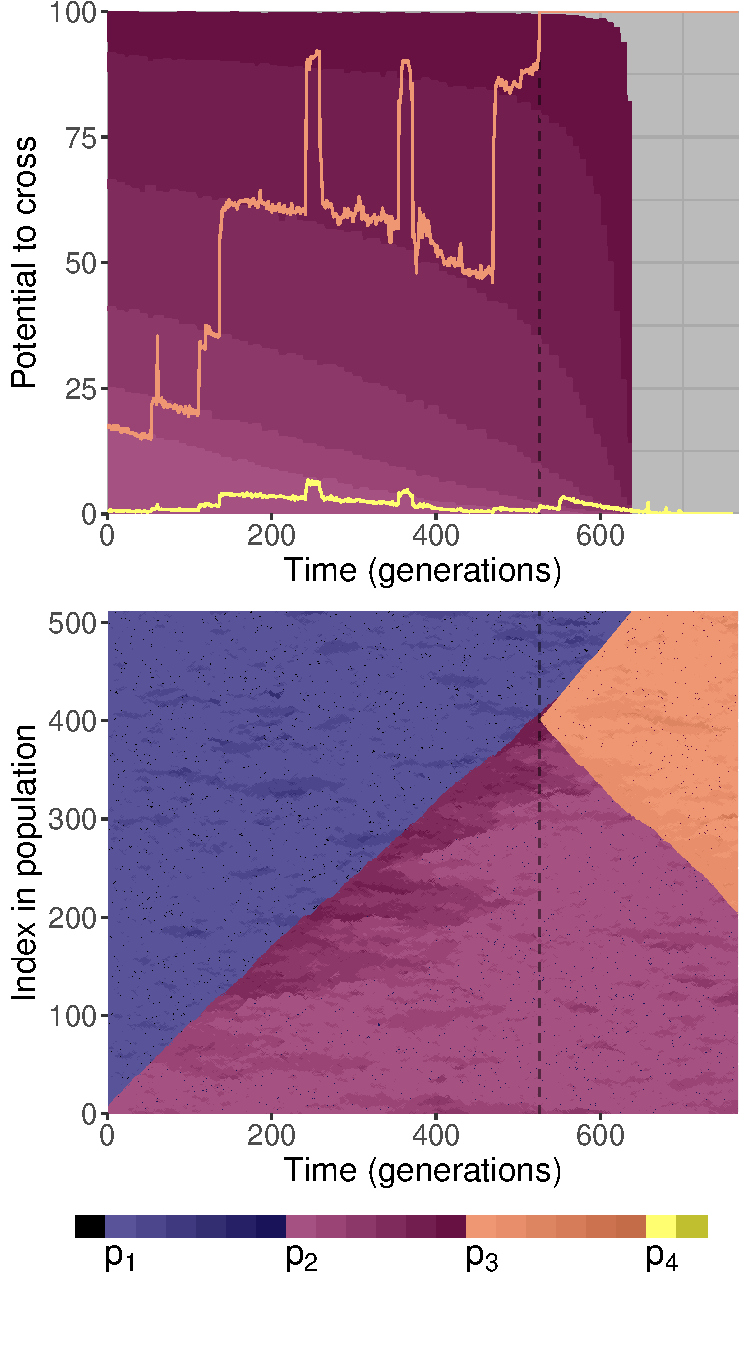
\includegraphics[width=0.6\textwidth]{05_adaptive_momentum/media/reps/400/script_06__plot_05__combined_plot_area_palette.pdf}
\caption{
    Top plot: Analytic replay data for a representative replicate that crossed one valley during a momentum window, overlayed on baseline data. 
    Lines show the probability of crossing both the first valley  (orange line; initially-higher) and the second valley (yellow line; initially-lower). 
    The background shows the expected potential to cross (as shown in Fig. \ref{fig-combined-plots}B); data here are shifted to align with the realized leading edge position. 
    %Each update was replayed 10,000 times. 
    Bottom plot: A Muller plot of all organisms in the original 1D population over time. 
    Dark colors show descent into valleys, with hue identifying the valley being crossed. 
    In both plots, vertical dashed lines show initial valley crosses.
    Colors in the legend apply to all plots. 
}
\label{fig-replay-single-cross}
\end{center}
\end{figure}

\begin{figure}[h!]
\begin{center}
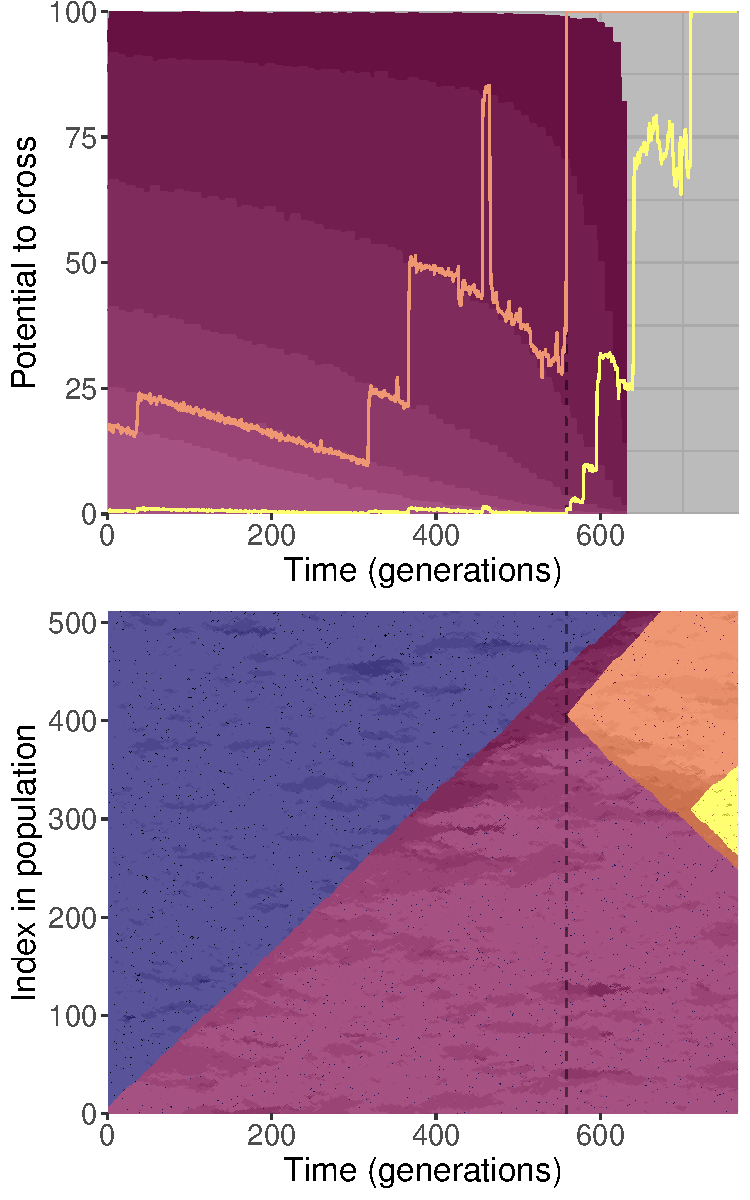
\includegraphics[width=0.6\textwidth]{05_adaptive_momentum/media/reps/263/script_06__plot_03__combined_plot_area.pdf}
\caption{
    The analytic replay data for a representative replicate that crossed two valleys during a momentum window. 
    See Figure \ref{fig-replay-single-cross} for details and legend. 
}
\label{fig-replay-double-cross}
\end{center}
\end{figure}

\begin{figure}[h!]
\begin{center}
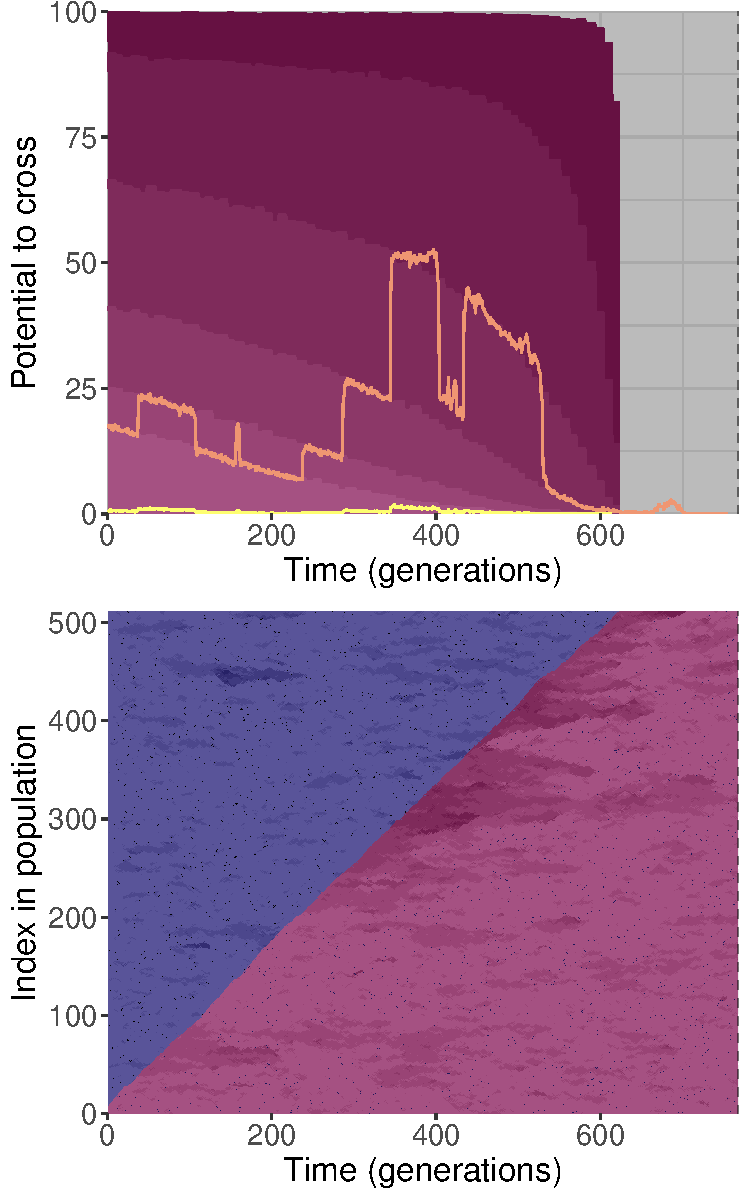
\includegraphics[width=0.6\textwidth]{05_adaptive_momentum/media/reps/339/script_06__plot_03__combined_plot_area.pdf}
\caption{
    The analytic replay data for a representative replicate that failed to cross a valley during a momentum window.
    See Figure \ref{fig-replay-single-cross} for details and legend.
}
\label{fig-replay-no-cross}
\end{center}
\end{figure}

For comparison, we also ran 10,000 replicates that started at equilibrium (\textit{i.e.}, not in a momentum window).
Of those, we replayed the one replicate that crossed twice, 10 randomly sampled replicates from 19 that crossed once, and 10 random replicates from the 9,980 that failed to cross. 
Figure \ref{fig-replay-no-window} shows the replicate that crossed twice. 
The first crossing in this replicate occurred quite early, crossing the valley on generation 168. 
However, the potential before crossing is similar to all first-cross replicates: while the potential in an adaptive momentum window starts at \localapprox 17\%, the potential for replicates outside momentum windows starts at \localapprox 0.2\%. 
This low potential continues for the first 143 generations, followed by 16 generations with an average potential of \localapprox 1.8\%, four generations between 15\% and 20\%, and then the cross. 
%This pure chance, ``all or nothing'' potentiation is not unique to this replicate, as we see in the histograms of potential shown in Figure \ref{fig-histograms}.
This pure chance, ``all or nothing'' potentiation is not unique to this replicate; the same dynamic can be seen in the ten other successful replicates we analyzed \citep{austin_ferguson_2024_11507982}.
% Figure \ref{fig-replay-no-window} shows the potential for the first and second valley crossing. 
% The potential for the first valley crossing remains very low ($<$0.4\%) until it increased to 100\% in less than 20 generations. 
% This increase is not linear, however, as there is an initial increase and then a drop in potentiation, likely corresponding to the flux in $p_{2} + 5$ organisms in the population. 
% The discovery of $p_{3}$ starts a momentum window, and the potential of the second cross then looks like the potential in previous results (although limited by the lack of remaining time), and is higher than the potential of the first window was for the first \localapprox 580 generations.


\begin{figure}[h!]
\begin{center}
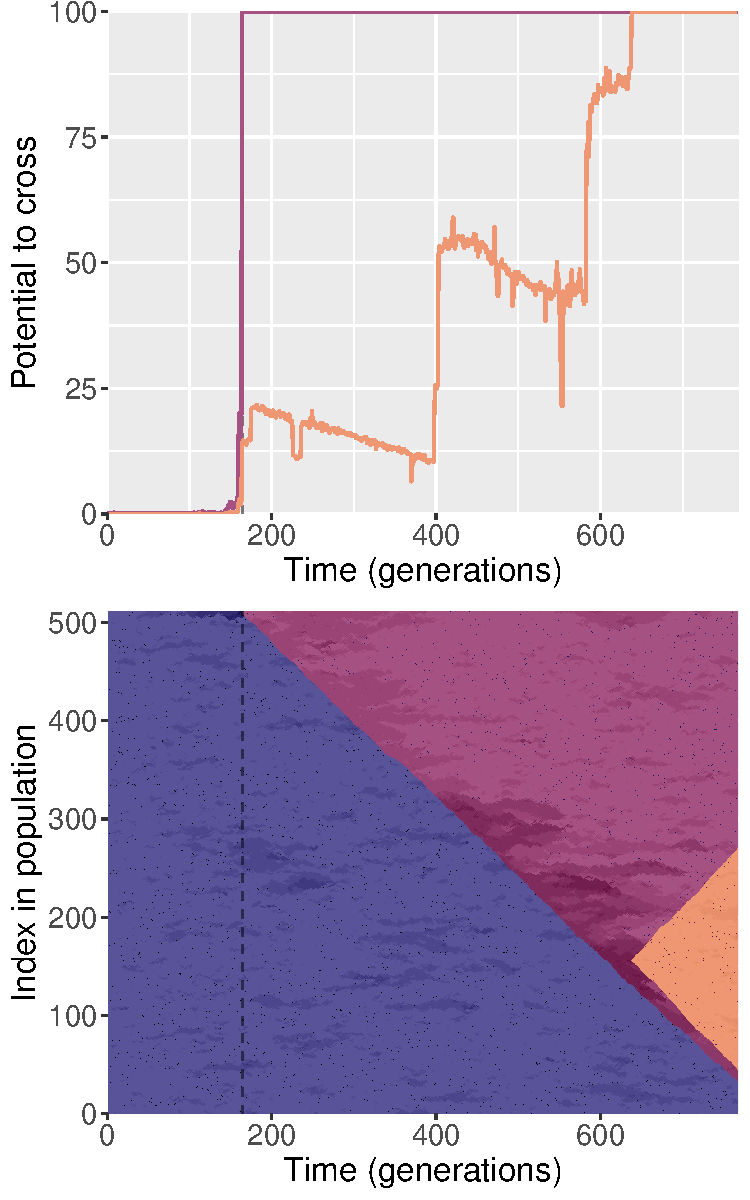
\includegraphics[width=0.6\textwidth]{05_adaptive_momentum/media/reps/no_am_two_cross/script_06__plot_02__combined_plot.pdf}
\caption{
    \textbf{Top plot}: The analytic replay data for the sole replicate that did \textit{not} start in a momentum window, but still managed to cross a valley, and indeed crossed twice. 
    The red line shows the potential to cross the first valley, while the orange line shows the potential to cross the second valley, exhibiting the hallmarks of adaptive momentum due to the first cross. 
    \textbf{Bottom plot}: a Muller plot of the original population, like in Figure \ref{fig-replay-single-cross}.
}
\label{fig-replay-no-window}
\end{center}
\end{figure}

Finally, we also show the potentiation of crossing the second valley, which in some cases is realized (Figs. \ref{fig-replay-double-cross} and \ref{fig-replay-no-window}), and other times is not (Figs. \ref{fig-replay-single-cross} and \ref{fig-replay-no-cross}).
As potentiation is probabilistic in nature, the potential to cross the second valley is the probability of crossing the first valley from the current state of the population times the probability of crossing a second valley from a na\"ive starting position (\textit{i.e.}, the elevated potentiation of a population at the beginning of a sweep). 
We see this dynamic early in the replays -- increases in first-cross potential are reflected, at smaller scales, in second-cross potential,
%Once the first valley is crossed, the potential to cross the second valley can increase dramatically. 
%Indeed, we see sizable increases in second-cross potential 
with a much larger increase upon successful crossing of the first valley in Figures \ref{fig-replay-single-cross} and \ref{fig-replay-double-cross}. %, \ref{fig-replay-no-window}, and . 
This result is consistent with the adaptive momentum framework, which posits that the discovery of a new peak will initiate a new adaptive momentum window. 
Strikingly, this same dynamic holds true for Figure \ref{fig-replay-no-window} -- while the replicate did not start in a momentum window, the first cross creates a window which increases the potential of the second cross.

\subsection{Shuffled population experiments}

To test the importance of population structure for potentiation, we repeated the benchmarking and replay experiments with shuffled populations. 
In both cases, we kept the experiments identical except for an additional shuffle step: before starting a replicate, we shuffled the order of organisms in the population and then proceeded with evolution as normal. 
%We replayed the evolution of 10 randomly-sampled single-cross replicates, and 

The shuffled benchmark data in Figure \ref{fig-combined-plots}C shows that only populations with a leading edge of $p_{2} + 5$ are able to maintain greater than a 10\% chance to cross if the leading edge has swept more than half the population.
Two differences can decrease crossing potential: 
1) multiple leading edges can form, allowing faster fixation and 
2) the eight leading-edge organisms are more likely to encounter higher-fitness mutant-type organisms and thus be purified faster.
%When the benchmark populations are shuffled, fixation occurs more rapidly and thus the potential to cross falls quickly.  

A representative sample from the single-cross replicates is shown in Figure \ref{fig-replay-shuffle}. 
The replay data indicate that potential to cross remains relatively low, never reaching a 20\% chance, until a critical mass of nearly-crossed organisms skyrockets the potential from 9.2\% to 100\%. 
The earlier spikes in potentiation always correspond to the appearance of a single organism that is one step away from crossing the valley, which was then lost in the original population.
These trends are consistent across all 10 replicates that were replayed \citep{austin_ferguson_2024_11507982}. 

\begin{figure}[h!]
\begin{center}
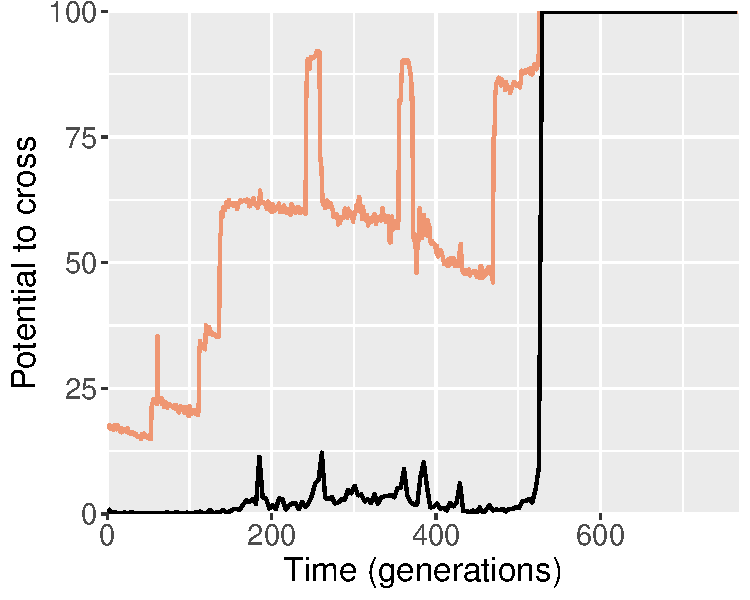
\includegraphics[width=0.6\textwidth]{05_adaptive_momentum/media/reps/400/script_07__plot_01__selected_replays_with_shuffled_replays_no_bg.pdf}
\caption{
    The black line (bottom) shows the potential for a shuffled population to cross a valley. 
    The orange line (top) shows the standard potential for the population to cross (same data as Fig. \ref{fig-replay-single-cross}). 
    The shuffled line consists of 1,000 samples every 4 generations. 
    %Background shading shows the expected potential to cross when an idealized leading edge population is shuffled (a shuffled version of Figure \ref{fig-benchmarking}). 
}
\label{fig-replay-shuffle}
\end{center}
\end{figure}

% \begin{figure}[h!]
% \begin{center}
% 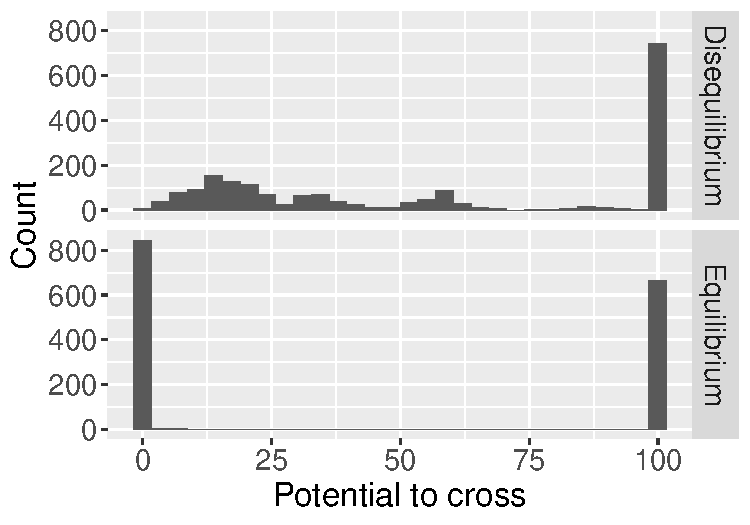
\includegraphics[width=0.45\textwidth]{media/combined_potentiation_histograms.pdf}
% \caption{
%     Histogram of potentiation values in replicates in a momentum window (disequilibrium, top) and outside a window (equilibrium, bottom).
% }
% \label{fig-histograms}
% \end{center}
% \end{figure}









% \section{Results}
% %Below we describe the results in the same order the experiments were described, first validating the adaptive momentum effect, then moving onto benchmarking and replay experiment results.  

% \begin{figure*}[h!]
% \begin{center}
% 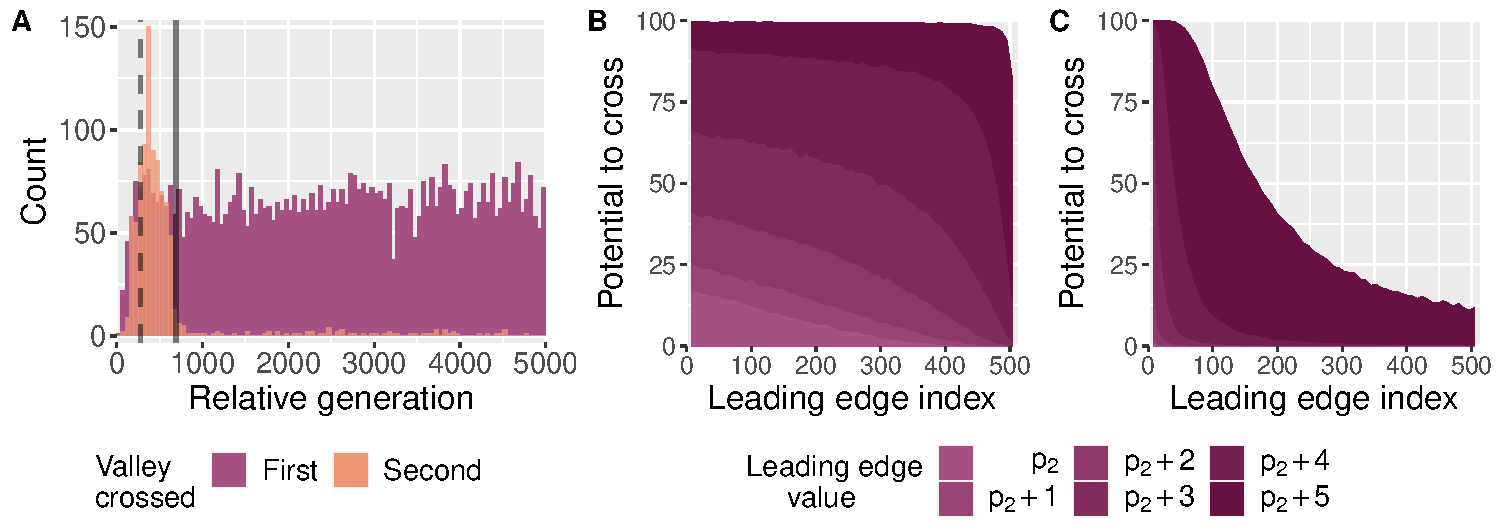
\includegraphics[width=\textwidth]{05_adaptive_momentum/media/combined_plots_full_split.pdf}
% \caption{
%     \textbf{(A)}
%     Distribution of the number of generations required to cross valleys in the validation experiment. 
%     Relative generations refer to the number of elapsed generations for the first cross, and the number of generations since the first cross for the second cross. 
%     %The solid and dashed horizontal lines show the expected count of first and second crosses per bar, respectively, for the expected uniform distribution. 
%     The dashed and solid vertical lines show the minimum and maximum fixation times, respectively. 
%     \textbf{(B)} 
%     Benchmarking data showing the potential of a leading edge to induce a valley cross, with a range of leading edge values and starting positions (see Figure \ref{fig-experiment2}). 
%     Each point represents 10,000 replicates.
%     \textbf{(C)}
%     Shuffled benchmarking data. Each replicate is shuffled prior to evolution, otherwise identical to center plot.
% }
% \label{fig-combined-plots}
% \end{center}
% \end{figure*}

% \subsection{Validation of adaptive momentum effect}

% First, we measured the time it took for replicates starting from a full population of $p_{2}$ to cross valleys.
% Figure \ref{fig-combined-plots}A
% shows the timing distributions of populations that crossed the first valley over the first 5,000 generations (red) as well as the timing distributions of second crossings that occur within 5,000 generations of a first (orange). 
% We see that the time of first crossing appear uniformly distributed across the 5,000 generations, while the second crosses are strongly biased toward shorter time periods. 
% Indeed, of 500,000 replicates, 6,485 crossed the first valley within 5,000 generations (\localapprox 1.3\%) with a mean cross time of \localapprox 2,569 generations and a median of 2,602 generations. 
% Based on these values, we would expect roughly 84 replicates to cross twice ($6,485 \times 1.3\%$, or 0.0169\% of all 500,000 replicates), but instead we see 902 replicates (\localapprox 0.18\%) cross the second valley, showing a much higher rate of second crossing than expected if the probabilities of first and second crossing were equal.
% In addition to a higher than expected rate of crossing, the mean cross time between first and second crossings is \localapprox 579 generations and the median cross time is 401 generations, substantially lower than the first crossing times. 
% Finally, when we consider only those second crossing times that occurred more than 1000 generations after a first crossing, we find that the rate of these second crossings is similar to the first crossing rate (\localapprox 1.23\%).
% These results comport with the framework of adaptive momentum. 
% They show that an initial beneficial discovery can quickly lead to additional discoveries (during the fixation period), but if the second discovery does not happen before equilibrium is reestablished, the rate of valley crossing is better predicted by the first valley crossing times. 


% % Indeed, of 500,000 replicates, 12,793 crossed at least once (\localapprox 2.6\%) with a mean cross time of \localapprox 4,995 generations and a median of 4,951 generations. 
% % We would expect that only 338 replicates to cross twice (2.6\% squared), but instead we see 1,734 replicates cross at least two valleys (\localapprox 0.35\% of total, or \localapprox 13.6\% of those that crossed once). 
% % For the second crossings, we see a mean cross time of 646 generations and a median cross time of 396 generations. 
% % Indeed, while not shown in Figure \ref{fig-crosses-from-scratch}, we see 200 replicates cross at least three valleys, 26 replicates cross at least four valleys, and six replicates cross five valleys; of these higher-order crossings, the median time to cross was always less than 420 generations. 
% % These findings, where an initial beneficial discovery can quickly lead to additional discoveries, supports the initial adaptive momentum theory. 

% % \begin{figure}[h!]
% % \begin{center}
% % 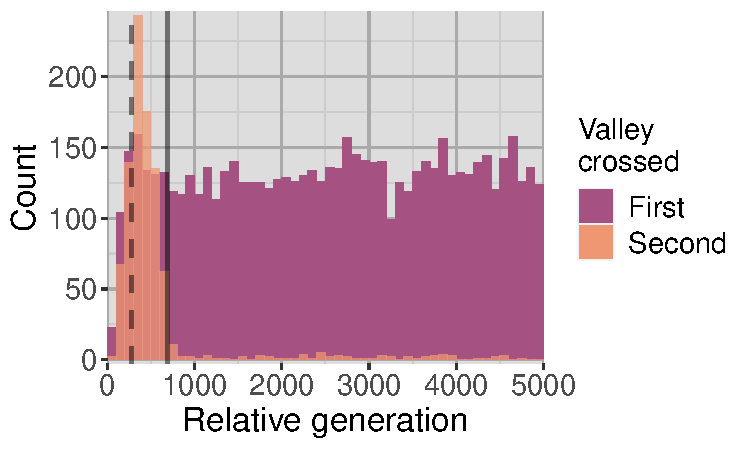
\includegraphics[width=0.45\textwidth]{media/first_two_crosses_overlayed_fair_comparison_with_fixation.pdf}
% % \caption{
% %     Distribution of the number of updates required to cross valleys in the validation experiment. 
% %     Relative updates refer to the number of elapsed generations for the first cross, and the number of generations since the first cross for the second cross. 
% %     %The solid and dashed horizontal lines show the expected count of first and second crosses per bar, respectively, for the expected uniform distribution. 
% %     The dashed and solid vertical lines show the minimum and maximum fixation times, respectively. 
% % }
% % \label{fig-crosses-from-scratch}
% % \end{center}
% % \end{figure}





% %Further, we tested the role of disequilibrium in these discoveries by comparing the evolution of populations seeded with eight organisms on $p_{2}$ and the rest on $p_{1}$ (disequilibrium treatment) against whole populations of $p_{2}$ (control). 
% %We found that 1,751 of 10,000 disequilibrium replicates crossed the first valley (\localapprox 17.5\%), while only 23 of 10,000 control replicates crossed (\localapprox 0.2\%). 
% %This difference is highly significant ($p < 10^{-15}$, Fisher's exact test).
% %This further supports the claim that adaptive momentum relies on disequilibrium in the population, and shows that we can start artificially start an adaptive momentum window in this system by creating this disequilibrium. 

% \subsection{Empirical benchmarks}

% %After confirming that disequilibrium can facilitate valley crosses, we next tested idealized populations to benchmark the effect on valley crossing of two components of this disequilibrium: the position of the leading edge, and the genotypes of the organisms comprising that leading edge.
% The empirical benchmark data (Figure \ref{fig-combined-plots}B) illustrate how the initial state of the population affects the potential to cross valleys.
% %In particular the ratio of the population initiated on $p_2$ (mutant type), versus $p_1$ (wild type) and the value of the individuals on the leading edge,
% As expected, steps further into the valley increase the probability of crossing, regardless of where the leading edge is. 
% On the other hand, the probability of crossing decreases as the ratio of $p_2$ organisms (mutant type) increases relative to $p_1$ organisms (wild type) -- as the selective sweep progresses there are fewer opportunities remaining for additional mutations to accumulate. 
% While the potential to cross varies considerably with the type of organisms in the leading edge, these data clearly show that all conditions describing early sweep conditions (i.e., having leading edge and a significant ratio of the remaining population on $p_1$) %having any leading edge 
% substantially increase the probability of crossing the valley compared to populations that are close to reaching equilibrium on $p_2$. 

% %The benchmarks with a leading edge at index 0 see slightly lower rates of crossing, as they only have one organism at the given value while every other point has 8 organ
% %We typically ran these benchmarking populations with a leading edge of eight organisms of the same type to remove the possibility of genetic drift immediately destroying the leading edge. 
% %This drift accounts for the drop in crosses at index 0, the one instance where the leading edge consisted of only a single organism. 
% %Finally, being one step away from crossing the valley ($p_2$ + 5) effectively guarantees a cross, as eight organisms at that value are almost certain to accumulate the one needed mutation unless the selective sweep is almost over. 
% %Overall, these data match our expectations. 
% We use these results to provide a baseline prediction for the analytic replay experiments. 

% % \begin{figure}[h!]
% % \begin{center}
% % 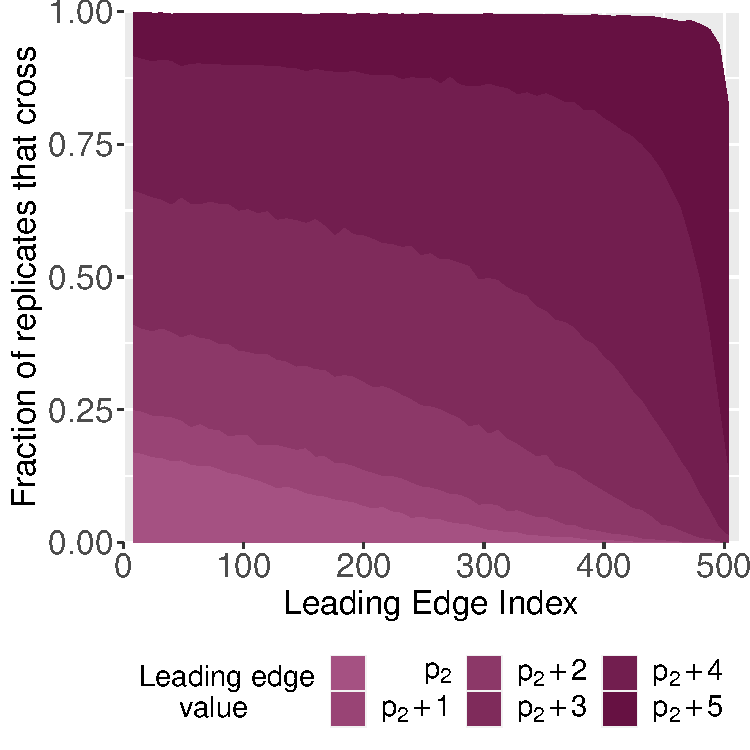
\includegraphics[width=0.45\textwidth]{media/benchmarking_area.pdf}
% % \caption{
% %     Benchmarking data showing the potential of a leading edge to induce a valley cross, with a range of leading edge values and starting positions. 
% %     The leading edge always consists of eight organisms of that value. 
% %     Each point represents 10,000 replicates. 
% % }
% % \label{fig-benchmarking}
% % \end{center}
% % \end{figure}

% \subsection{Analytic replay experiments}
% Of our 500 initial replicates to find candidates for replay experiments, four replicates (0.8\%) crossed two valleys in the allotted time, 83 crossed exactly one valley (16.6\%), and the remaining 413 did not cross any valleys (82.6\%). 
% We ran coarse-grained replays for 10 randomly-sampled no-cross replicates, 10 random single-cross replicates, and all four double-cross replicates.
% %We ran coarse-grained analytic replay experiments for all four replicates that crossed twice and for 10 randomly-sampled replicates of each of the two other categories. 
% %For each of these 24 replicates, we replayed at every fourth generation, with 1,000 replicates per time point. 
% All plots are available in the supplement \citep{austin_ferguson_2024_11507982}. 

% From these coarse-grained replays, we selected one representative replicate from each category. 
% We re-ran these representative replicates, conducting 10,000 replay trials at \textit{every} time point to give a fine-grained view. 
% %We show the replay results in two formats. 
% %The first showing the potential of crossing the next valley over time and the second as Muller plots showing the underlying population structure that beget that potentiation. 
% For each replayed replicate, we show the potential of crossing the next valley over time, paired with a Muller plot \citep{mullerGeneticAspectsSex1932} of the initial replicate that was replayed. 
% Figures \ref{fig-replay-single-cross}, \ref{fig-replay-double-cross}, and \ref{fig-replay-no-cross} show the single-cross, double-cross, and no-cross replicates, respectively. 
% %In each plot, the replay results are overlaid atop the benchmarking data, which has been adjusted such that the leading edge index aligns with the actual leading edge at that generation of the population.
% In each plot, the replay results are overlaid atop an image generated from the benchmark data. 
% %To generate the background image, we treat the benchmark data as a lookup function and use the current position of the leading edge of the replay result to look up the potentiation predicted by the benchmark data. 
% To generate the background image, we treat the benchmark data as a lookup function. 
% When we start a replay replicate, we initialize the population using the snapshot from a particular generation of the initial replicate. 
% These snapshots show that the leading edge does not perfectly advance one position every generation; there are many generations where the leading edge either fails to advance or is pushed back one position by the wild type organisms.
% %As we see in our population snapshots, the leading edge does not actually advance one position every generation, the leading often fails to advance, and occasionally the wild-type organisms replicate over the leading edge, pushing it back one step. 
% To make this comparison fair, we find the leading edge in that particular snapshot and then look up the corresponding expectation values from the benchmark data. 
% %Thus, the background image shows in ``real time'' potentiation of the replay at each generation.
% This adjustment ensures that we are comparing against the correct benchmark data regardless of the motion of the leading edge. 
% %Thus, the background image adjusts 

% Overall, the potentiation observed in all three replicates closely match the benchmark expectations. 
% The potentiation occasionally increases or decreases suddenly; tracing these changes to the Muller plots typically shows that these events correlate to the gain or loss of a mutation at (or near) the leading edge at that time. 
% For example, the two temporary peaks in potential in Figure \ref{fig-replay-single-cross}, at roughly generations 250 and 375, can be directly traced to the leading edge temporarily dipping to $p_{2} + 4$.
% %When the leading edge mutates further into the fitness valley, the potentiation increases dramatically. 
% %Each of the three replicates 
% The potentiation at any particular step in the valley decreases over time, as the selective sweep progresses and the adaptive momentum window closes.
% Figure \ref{fig-replay-no-cross} clearly shows that, while the replicate had substantial potentiation at times (briefly above 50\%), it failed to capitalize before the window closed. 
% This failure was exacerbated by two leading mutations from $p_{2} + 3$ to $p_{2} + 2$, the second of which dropped the potential from over 25\% to under 10\%, after which the population never recovers. 
% % It should be noted that the dramatic increases or decreases in potentiation can be mapped cleanly onto the Muller plots showing the state of the population. 
% % For example, in Figure \ref{fig-replay-single-cross} potentiation temporarily increases dramatically (from \localapprox 60\% to \localapprox 90\%) twice, once around update 250 and again around update 350. 
% % In both cases, the potentiation then drops to previous levels shortly after. 
% % Mapping this points onto the Muller plot, we see that, in both cases, the leading edge drifted down an additional step into the valley (to $p_{1} + 4$) before quickly drifting back to the previous step. 
% % These drops in potentiation are particularly dramatic in the no-cross replicate of Figure \ref{fig-replay-no-cross}, where a late drift backward reduces the potential to cross from over 25\% to under 10\%, from which the population never recovers. 

% All three replicates show periods of potentiation higher than what our benchmark data would predict given their leading edge genomic value. 
% The benchmarking data modeled a leading edge of eight organisms, but the Muller plots show that the leading edge grows and shrinks over time. 
% The Muller plots show that overprediction is generally associated with either an expanded leading edge or an excess of individuals with lower fitness behind the leading edge. 
% We hypothesized that these overpredictions are generally observed in deeper steps into the valley because of the historical contingency required to reach that point (i.e., to reach $p_{2} + 5$ the leading edge must have passed through $p_{2} + 4$, which may still exist behind the leading edge).
% %While all organisms behind the leading edge are experiencing purifying selection, this purification takes time, and a cluster of mutated organisms can persist behind the leading edge. 
% %Our benchmark expectations are particularly accurate for early steps into the valley; even if a large cluster of organisms exists behind the leading edge, they are still unlikely to accumulate the needed mutations to cross the valley before being purified. 
% %In contrast, when the leading edge is only a mutation or two away from crossing, even a few organisms trailing the leading edge can be enough to cross the valley. 
% %If a sizable section of the population is only two or three mutations from crossing the valley, the size of that section may buffer the organisms from purifying selection long enough for some organisms to genetically drift to the next peak. 
% %This is supported by the replays almost perfectly aligning with the expectation in the first few steps into the valley, where the mutation rate cannot outpace the rate of purifying selection, while the empirical potentiation is often above the expectation in the last few steps of the valley. 
% %This was not explicitly modeled in the benchmarking data, possibly causing this difference. 
% %while replays see leading edges that are much larger or smaller, causing some variation from the expectation.
% %Further, our benchmarks are based \textit{only} on the leading edge, and thus our hypothesis is that this higher-than-expected potentiation results from the evolutionary potential of non-leading edge organisms. 

% \begin{figure}[h!]
% \begin{center}
% 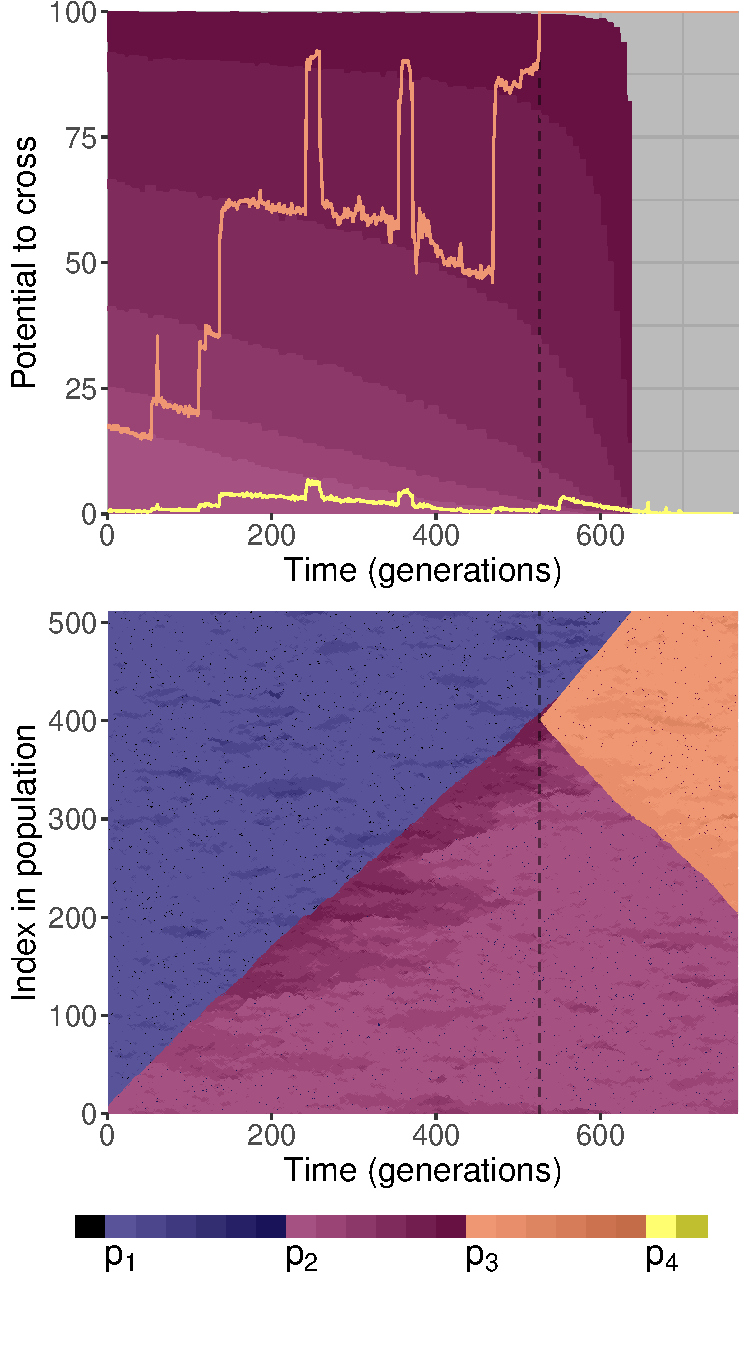
\includegraphics[width=0.6\textwidth]{05_adaptive_momentum/media/reps/400/script_06__plot_05__combined_plot_area_palette.pdf}
% \caption{
%     \textbf{Top plot}: The analytic replay data for a representative replicate that crossed one valley during a momentum window. 
%     The two lines show the probability of crossing valleys, with the initially-higher (orange) line showing the first valley cross and the initially-lower (yellow) line showing the second valley cross. 
%     The background shading shows the expected potential to cross (as shown in Figure \ref{fig-combined-plots}B), adjusted by the actual leading edge of the population. 
%     Each update was replayed 10,000 times. 
%     \textbf{Bottom plot}: A Muller plot of the original population over time. 
%     Dark colors show descent into a valley, with hue identifying the valley being crossed. 
%     In both plots, vertical lines show valley crosses.
%     Colors in the legend apply to all plots. 
% }
% \label{fig-replay-single-cross}
% \end{center}
% \end{figure}

% \begin{figure}[h!]
% \begin{center}
% 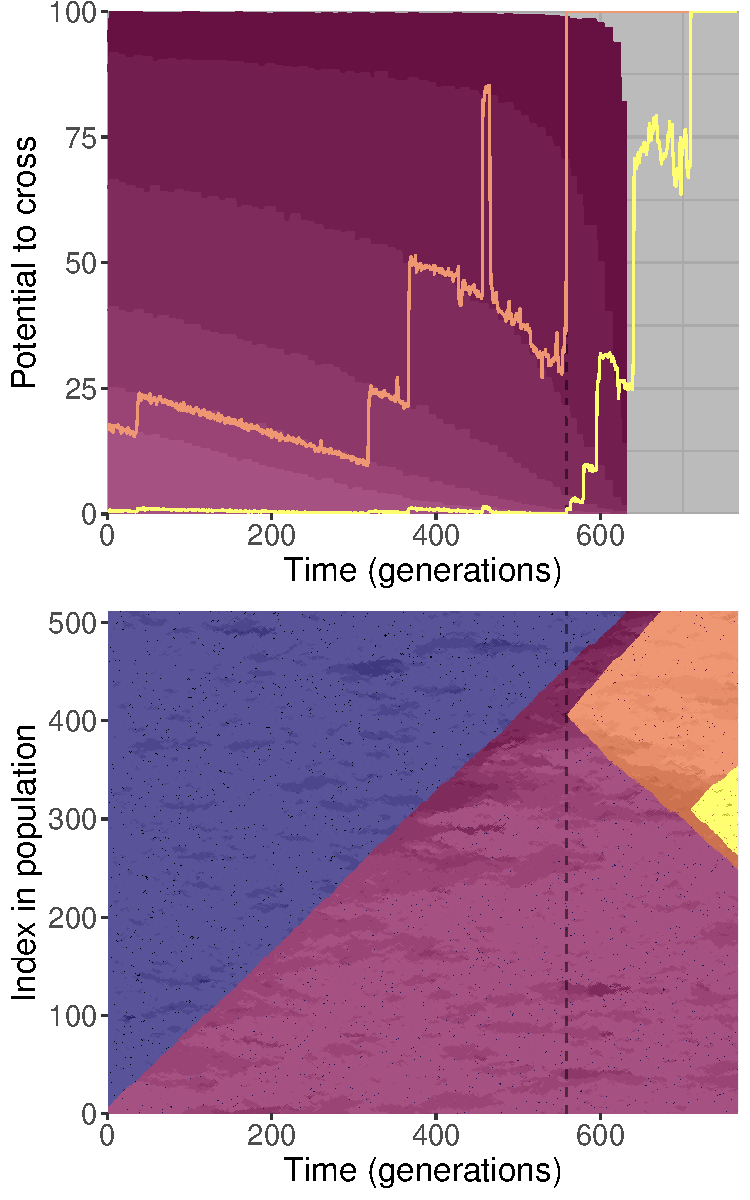
\includegraphics[width=0.6\textwidth]{05_adaptive_momentum/media/reps/263/script_06__plot_03__combined_plot_area.pdf}
% \caption{
%     The analytic replay data for a representative replicate that crossed two valleys during a momentum window. 
%     See Figure \ref{fig-replay-single-cross} for details and legend. 
% }
% \label{fig-replay-double-cross}
% \end{center}
% \end{figure}

% \begin{figure}[h!]
% \begin{center}
% 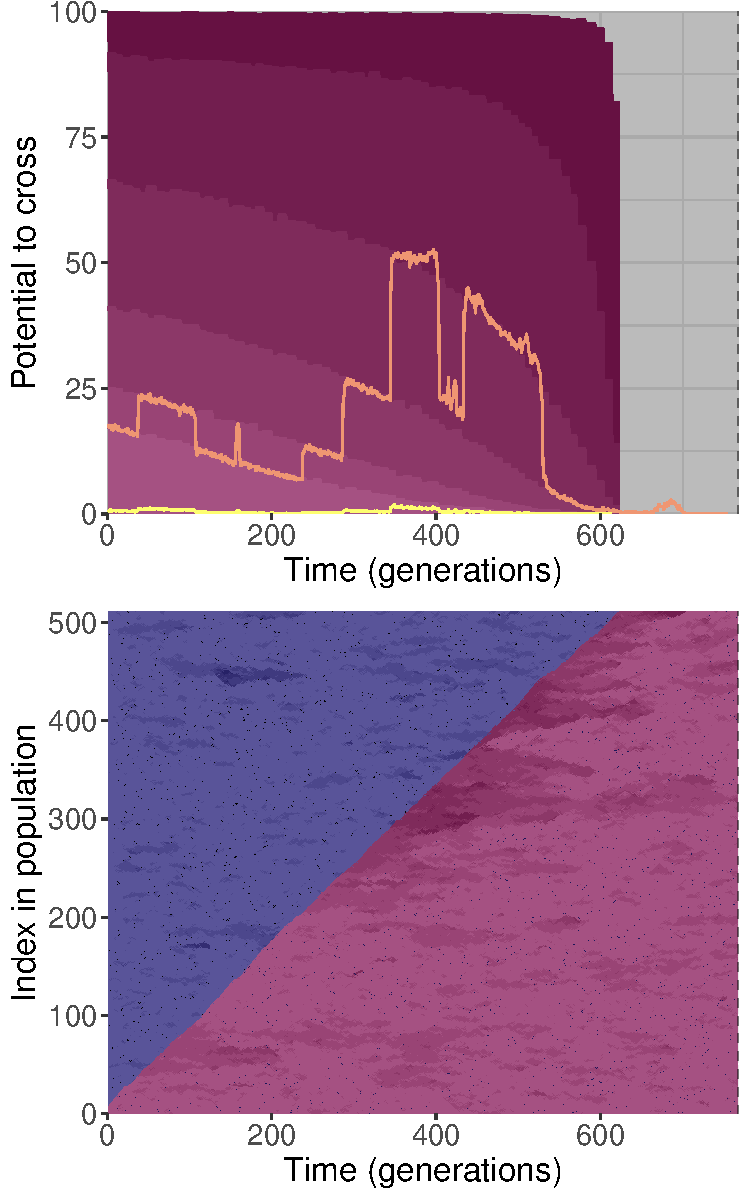
\includegraphics[width=0.6\textwidth]{05_adaptive_momentum/media/reps/339/script_06__plot_03__combined_plot_area.pdf}
% \caption{
%     The analytic replay data for a representative replicate that failed to cross a valley during a momentum window.
%     See Figure \ref{fig-replay-single-cross} for details and legend.
% }
% \label{fig-replay-no-cross}
% \end{center}
% \end{figure}

% For comparison, we also replayed replicates that did not start in a momentum window. 
% We replayed the one replicate in 10,000 that crossed twice, 10 randomly sampled replicates that crossed once, and 10 random replicates that failed to cross. 
% Figure \ref{fig-replay-no-window} shows the replicate that crossed twice. 
% The first crossing in this replicate occurred quite early, crossing the valley on generation 168. 
% However, the potential before crossing is similar to all first-cross replicates: while the potential in an adaptive momentum window starts at \localapprox 17\%, the potential for replicates outside momentum windows starts at \localapprox 0.2\%. 
% This low potential continues for the first 143 generations, followed by 16 generations with an average potential of \localapprox 1.8\%, four generations between 15\% and 20\%, and then the cross. 
% %This pure chance, ``all or nothing'' potentiation is not unique to this replicate, as we see in the histograms of potential shown in Figure \ref{fig-histograms}.
% This pure chance, ``all or nothing'' potentiation is not unique to this replicate; the same dynamic can be seen in the ten other succesful replicates we analyzed \citep{austin_ferguson_2024_11507982}.
% % Figure \ref{fig-replay-no-window} shows the potential for the first and second valley crossing. 
% % The potential for the first valley crossing remains very low ($<$0.4\%) until it increased to 100\% in less than 20 generations. 
% % This increase is not linear, however, as there is an initial increase and then a drop in potentiation, likely corresponding to the flux in $p_{2} + 5$ organisms in the population. 
% % The discovery of $p_{3}$ starts a momentum window, and the potential of the second cross then looks like the potential in previous results (although limited by the lack of remaining time), and is higher than the potential of the first window was for the first \localapprox 580 generations.


% \begin{figure}[h!]
% \begin{center}
% 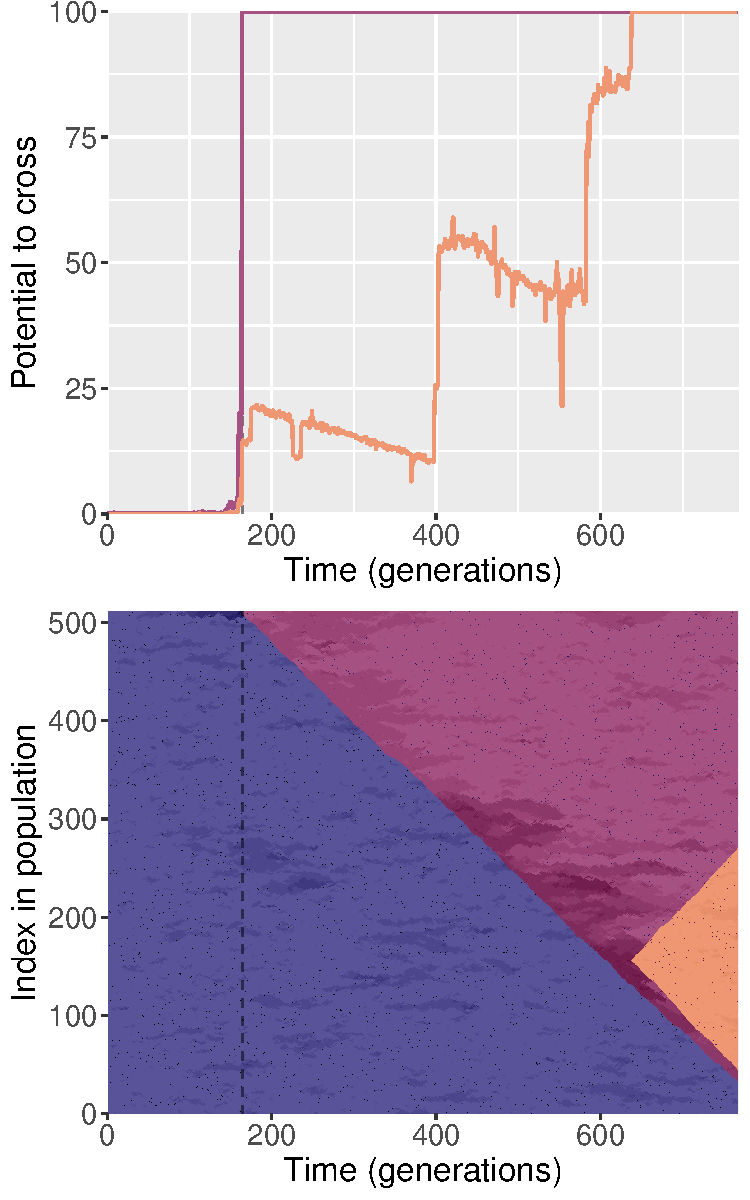
\includegraphics[width=0.6\textwidth]{05_adaptive_momentum/media/reps/no_am_two_cross/script_06__plot_02__combined_plot.pdf}
% \caption{
%     \textbf{Top plot}: The analytic replay data for a representative replicate that did \textit{not} start in a momentum window but still managed to cross a valley. 
%     The red line shows the potential to cross the first valley, while the orange line shows the potential to cross the second valley. 
%     \textbf{Bottom plot}: a Muller plot of the original population, like in Figure \ref{fig-replay-single-cross}.
% }
% \label{fig-replay-no-window}
% \end{center}
% \end{figure}

% Finally, we also show the potentiation of crossing the second valley, which in some cases is realized (as in Figures \ref{fig-replay-double-cross} and \ref{fig-replay-no-window}), and other times is not (Figures \ref{fig-replay-single-cross} and \ref{fig-replay-no-cross}).
% As potentiation is probabilistic in nature, the potential to cross the second valley can be thought of as the product of crossing the first valley from the current state of the population and the probability of crossing a second valley from a naive starting position (i.e, the elevated potentiation of a population at the beginning of a sweep). 
% We see this dynamic reflected early in the replays -- increases in first-cross potential are reflected, at much smaller scales, in second-cross potential. 
% Once the first valley is crossed, the potential to cross the second valley can increase dramatically. 
% We see sizable increases in second-cross potential upon successful crossing of the first valley in Figures \ref{fig-replay-single-cross} and \ref{fig-replay-double-cross}. %, \ref{fig-replay-no-window}, and . 
% This result is consistent with adaptive momentum framework, which posits that the discovery of a new peak will initiate a new adaptive momentum window. 
% Most strikingly, this same dynamic holds true for Figure \ref{fig-replay-no-window} -- while the replicate did not start in a momentum window, we see the first cross create a window and the potential of the second cross reflects that.

% \subsection{Shuffled population experiments}

% To test the effect of population structure on potentiation, we repeated the benchmarking and replay experiments with shuffled populations. 
% In both cases, the experiments were repeated exactly, except for one additional shuffle step: before beginning to evolve the populations, we would shuffle the order of organisms in the population, and then proceed with evolution as normal. 
% %We replayed the evolution of 10 randomly-sampled single-cross replicates, and 

% The shuffled benchmark data in Figure \ref{fig-combined-plots}C shows that only populations with a leading edge of $p_{2} + 5$ are able to maintain greater than a 10\% chance to cross if the leading edge has swept more than half the population.
% Two differences arise when we shuffle the benchmark populations that can decrease crossing potential: 
% 1) fixation can occur faster because of multiple leading edges and 
% 2) when the eight organisms from the leading edge are shuffled into the population, they are likely to be purified faster.
% %When the benchmark populations are shuffled, fixation occurs more rapidly and thus the potential to cross falls quickly.  

% A representative sample from the 10 single-cross replicates is shown in Figure \ref{fig-replay-shuffle}. 
% The replay data indicate that potential to cross remains relatively low, never reaching a 20\% chance, until a critical mass of nearly-crossed organisms skyrockets the potential from 9.2\% to 100\%. 
% The earlier spikes in potentiation always correspond to the appearance of a single organism that is one step away from crossing the valley, which was then lost in the original population.
% These trends were consistent across all 10 replicates that were replayed \citep{austin_ferguson_2024_11507982}. 

% \begin{figure}[h!]
% \begin{center}
% 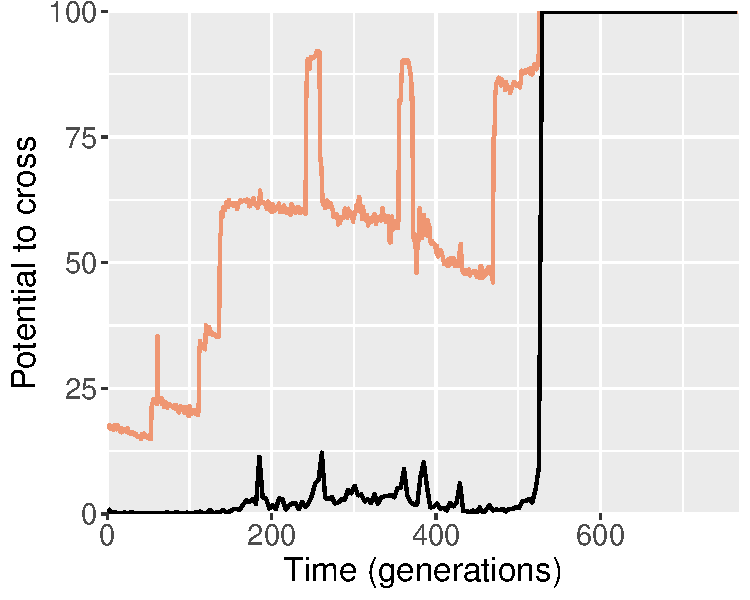
\includegraphics[width=0.6\textwidth]{05_adaptive_momentum/media/reps/400/script_07__plot_01__selected_replays_with_shuffled_replays_no_bg.pdf}
% \caption{
%     The black line (bottom) shows the potential for a shuffled population to cross a valley. 
%     The orange line (top) shows the standard potential for the population to cross (same data as Figure \ref{fig-replay-single-cross}). 
%     The shuffled line consists of 1,000 samples every 4 generations. 
%     %Background shading shows the expected potential to cross when an idealized leading edge population is shuffled (a shuffled version of Figure \ref{fig-benchmarking}). 
% }
% \label{fig-replay-shuffle}
% \end{center}
% \end{figure}

% % \begin{figure}[h!]
% % \begin{center}
% % 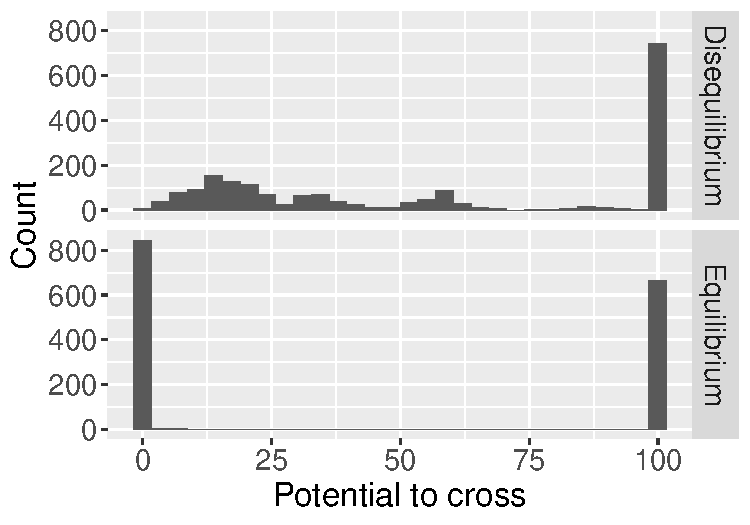
\includegraphics[width=0.45\textwidth]{media/combined_potentiation_histograms.pdf}
% % \caption{
% %     Histogram of potentiation values in replicates in a momentum window (disequilibrium, top) and outside a window (equilibrium, bottom).
% % }
% % \label{fig-histograms}
% % \end{center}
% % \end{figure}


\section{Discussion and Conclusion}

% Crossing is pure chance without AM
%   But has some baseline probability under AM
%\subsection{Adaptive momentum can drastically alter a population's potential}
\subsection{Potentiation exhibits adaptive momentum}

In this work, we have corroborated adaptive momentum's benefit to valley crossing (as outlined in \citep{Bohm2024.04.08.588357}) and expanded our understanding of the dynamic. 
Our initial experiments demonstrated that our system can undergo adaptive momentum, and that disequilibrium is the key driver. 
However, our main goal in this paper is to provide an alternate vantage point from which to view the dynamics of adaptive momentum. 
While the original paper validated the effect via aggregated data, here we analyze the underlying dynamics in action on individual populations by quantifying potentiation via replay experiments. 

We have shown that populations outside of momentum windows must rely on chance alone to cross a valley. 
During these ``equilibrium'' periods, early mutations into the valley, although required for a valley crossing, have no substantial impact on the population's probability of crossing. 
Conversely, populations in momentum windows immediately see a drastically higher chance to cross, and every mutation in the leading edge is either potentiating or anti-potentiating, depending on the direction. 
This result is highlighted in Figure \ref{fig-replay-no-window}, where the first cross was pure chance while the second cross was driven by adaptive momentum.
This work is only a beginning; future work should apply these techniques to examine the role of adaptive momentum in more complex and realistic fitness landscapes.

% Do we need something to tie this section together


% The leading edge value almost perfectly predicts potentiation for the first few steps
\subsection{The leading edge in a spatial selective sweep determines potentiation}
%\subsection{The position and state of the leading edge of a selective sweep determines its adaptive potential}

The adaptive momentum framework posits that disequilibrium in a population can reduce the selection pressure on the advantaged subpopulation \citep{Bohm2024.04.08.588357}.
In spatial populations, disequilibrium is focused at the leading edge of selective sweeps, where advantaged mutants encroach on the wild type. %, which is exactly what we see here. 
Indeed, we observe that the genotype of the organism at the leading edge of the sweep is a strong predictor of potentiation. 
Moreover, as we can see in the Muller plots, there are often mutated organisms lagging the leading edge. 
When the leading edge is further into the valley, those lagging organisms have a non-negligible chance to accumulate sufficient mutations to finish crossing the valley, thus increasing the potential.

We aimed to create the simplest system for studying valley crossing in spatial populations.
In these one-dimensional populations, our artificially-started sweeps have exactly one leading edge. % (although self-actuated sweeps may have two or more). 
These edges become more complex in two-dimensional digital systems and only increase in complexity moving toward more natural systems. 
While the identification and measurements of the leading edge may become more difficult, we expect similar dynamics to hold. 
It is critical that we continue to improve our understanding of adaptive momentum in these simple systems to build a solid theoretical foundation. 
%We expect that similar dynamics will unfurl in these more complicated systems, but with many more intricacies. 
%For example, here our potential to cross in a momentum window moves in predictable and sizable steps because we have only one organism at the leading edge. 
%In more complex systems, these dynamics will be much harder to identify. 


% When we take population snapshots, potentiation looks great
%   If we shuffle the population, potentiation is very low until we cross
%   If we do clonal restarts, potentiation is only ever ~0% and ~100%
\subsection{Population heterogeneity and structure affect potentiation}

Previous experiments have conducted analytic replays starting from clonal populations \citep{blountHistoricalContingencyEvolution2008, fergusonPotentiatingMutationsFacilitate2023}. 
Here, however, we used perfect population snapshots that record every organism in every generation. 
Our technique provides a more fine-grained look into how potentiation changes. 
%In fact, if we had started with clonal populations of the most abundant genotype as in previous work, we would only see a maximum of four clones per replicate ($p_{1}$, $p_{2}$, $p_{3}$, and $p_{4}$) because at no time during any of our experiments is the dominant type in a population not a purebred type.
Furthermore, previous work has often used the most abundant genotype at a time point to seed replay experiments. 
Across all of our experiments, the most abundant genotype was always on one of the peaks. % ($p_{1}$, $p_{2}$, $p_{3}$, or $p_{4}$).
Replays looking at the potential of the first cross would see effectively zero probability for $p_{1}$ and $p_{2}$ and 100\% probability for $p_{3}$ and $p_{4}$, which have already crossed, missing all nuance and change in this potential. 

The nuance gained by replaying population snapshots provides important insight into using analytic replay experiments, and puts the large jumps in potentiation seen in previous work into question \citep{fergusonPotentiatingMutationsFacilitate2023}.
While those large jumps in potentiation are valid, they are likely missing important intermediate genotypes or population dynamics. 
In effect, they show genetic effects isolated from effects of population structure.
%Future work should use population snapshots when possible, and further analysis into the effect of using population snapshots instead of clonal restarts should be further disentangled in simple models like this one. 
Future work looking to leverage replay experiments should be aware that population structure and composition can affect evolutionary outcomes, and should thus carefully consider how replays are initialized. 
%This work signifies the first step in using genetic potentiation to study population dynamics. 

Further, by shuffling the population snapshots we have shown that it is not just the portion of the population with each genotype that matters, but also the structural relationships and interactions among the organisms (Figure \ref{fig-replay-shuffle}).
Other computational studies will likely be needed to tease apart when and how this organization matters %; however, while replay experiments of natural organisms are always monumental amounts of work, 
as perfectly preserving structure and composition of natural populations for so many replicates is currently impossible. 
As such, we should leverage computational models to develop techniques possible in both digital and natural populations, possibly finding a middle ground between a single clonal sample and full population snapshots. 
%The organization of the population matters in two ways: 1) preservation of the leading edge and 2) formation of ``depressed'' region. 
%When we shuffle a population, the leading edge might have fewer organisms left to sweep and thus fewer opportunities for mutations, or, worse, be isolated to only a few organisms that are then purged by purifying selection or genetic drift. 
%As we see in Figure \ref{fig-replay-double-cross}, valley crosses sometimes occur slightly behind the leading edge in a mutated region that has not yet been subjected to purifying selection. 
%In these cases, the size of the region matters -- the more organisms in it the longer it will take for them all to be purified. 
%We have shown that when we shuffle the population, we are destroying these regions and thus limiting potential to cross. 

\subsection{Outlook}


%This work not only serves to replicate the expectations of adaptive momentum, but effectively exposes the underlying mechanisms. 
%By quantifying potentiating and relating this to population composition and structure, we have strengthened the arguments proposed by adaptive momentum theory while also expanding the use cases for potentiation and replay experiments as analytical tools.

This work not only provides evidence to support our understanding of adaptive momentum, but further clarifies the underlying mechanisms. 
By quantifying the potentiation of valley crosses and relating this measure to population composition and structure, we have % strengthened the arguments proposed in the adaptive momentum framework and 
provided insights into the historical contingencies and long-term trajectories of populations experiencing adaptive momentum. 
Further, we advance the methodology of analytic replay experiments by conducting them at a greater scale than previously seen, demonstrating a new use case, and leveraging perfect population snapshots to seed the replay experiments. 
These advances combine to show that replay experiments can extend genetic potentiation to include the effects of population dynamics. 
All together, this work constitutes both a step toward better understanding adaptive momentum and a methodological refinement of replay experiments for understanding historical contingency.












% \section{Discussion and Conclusion}

% % Crossing is pure chance without AM
% %   But has some baseline probability under AM
% %\subsection{Adaptive momentum can drastically alter a population's potential}
% \subsection{Potentiation exhibits adaptive momentum}

% In this work, we have corroborated adaptive momentum's benefit to valley crossing originally outlined in \citep{Bohm2024.04.08.588357}. 
% Our initial experiments demonstrated that our system can experience adaptive momentum, and that disequilibrium is the key driver. 
% However, the main goal of this paper is to provide an alternative vantage point from which to view the dynamics of adaptive momentum. 
% While the original paper validated the effect via aggregated data, here we analyze the underlying dynamics in action on individual populations by quantifying potentiation via replay experiments. 

% We have shown that populations outside of momentum windows must rely on chance alone to cross the valley. 
% During these ``equilibrium'' periods, early mutations into the valley, although required for a valley crossing, have no substantial impact on the population's probability of crossing. 
% Conversely, populations in momentum windows immediately see a drastically higher chance to cross, and every mutation in the leading edge is either potentiating or anti-potentiating, depending on the direction. 
% This is highlighted in Figure \ref{fig-replay-no-window}, where the first cross was pure chance while the second cross was driven by adaptive momentum.
% This work is only the beginning, and future work should apply similar techniques to understanding the role of adaptive momentum in other, more complex, fitness landscapes.

% % Do we need something to tie this section together


% % The leading edge value almost perfectly predicts potentiation for the first few steps
% \subsection{The leading edge in a spatial selective sweep determines potentiation}
% %\subsection{The position and state of the leading edge of a selective sweep determines its adaptive potential}

% The adaptive momentum framework posits that disequilibrium in a population can reduce the selection pressure on the advantaged subpopulation \citep{Bohm2024.04.08.588357}.
% In a spatial populations, disequilibrium is focused at the leading edge of selective sweeps, where the advantaged mutants will continue to encroach on the wild type. %, which is exactly what we see here. 
% Indeed, we observe that the genotype of the organism at the leading edge of the sweep is a strong predictor of potentiation in this system. 
% Moreover, as we can see in the Muller plots, there is often a cluster of mutated organisms lagging the leading edge. 
% When the leading edge is further into the valley and fewer mutations are needed to cross, those lagging organisms have a non-negligible chance to accumulate sufficient mutations and cross the valley, increasing the potential.

% We aimed to create the simplest system for studying the leading edge of spatial populations.
% In these one-dimensional populations, our artificially-started sweeps have exactly one leading edge. % (although self-actuated sweeps may have two or more). 
% These edges become more complex in two-dimensional digital systems and only increase in complexity moving toward more natural systems. 
% While the identification and use of the leading edge for making predictions may become more difficult, we expect similar dynamics to hold. 
% It is critical that we continue to improve our understanding of adaptive momentum in these simple systems to build a solid foundation to expand upon. 
% %We expect that similar dynamics will unfurl in these more complicated systems, but with many more intricacies. 
% %For example, here our potential to cross in a momentum window moves in predictable and sizable steps because we have only one organism at the leading edge. 
% %In more complex systems, these dynamics will be much harder to identify. 


% % When we take population snapshots, potentiation looks great
% %   If we shuffle the population, potentiation is very low until we cross
% %   If we do clonal restarts, potentiation is only ever ~0% and ~100%
% \subsection{Population heterogeneity and structure affect potentiation}

% Previous work using analytic replay experiments have started the replays with clonal populations \citep{blountHistoricalContingencyEvolution2008, fergusonPotentiatingMutationsFacilitate2023}. 
% Here, however, we ran replays with perfect population snapshots that record every organism in every generation. 
% This technique provides a more fine-grained look into how potentiation changes. 
% %In fact, if we had started with clonal populations of the most abundant genotype as in previous work, we would only see a maximum of four clones per replicate ($p_{1}$, $p_{2}$, $p_{3}$, and $p_{4}$) because at no time during any of our experiments is the dominant type in a population not a purebred type.
% Previous work has used the most abundant organism at a time point to seed replay experiments. 
% Across all of our experiments, the most abundant organism type was always on one of the peaks. % ($p_{1}$, $p_{2}$, $p_{3}$, or $p_{4}$).
% Replays looking at the potential of the first cross would see effectively zero probability for $p_{1}$ and $p_{2}$ and 100\% probability for $p_{3}$ and $p_{4}$, which have already crossed, missing all nuance and change in this potential. 

% The nuance gained by replaying population snapshots provides important insight into using analytic replay experiments, and puts the large jumps in potentiation seen in previous work into question \citep{fergusonPotentiatingMutationsFacilitate2023}.
% While those large jumps in potentiation are valid, they are likely missing important intermediate genotypes or population dynamics. 
% In effect, they show genetic effects isolated from effects of population structure.
% %Future work should use population snapshots when possible, and further analysis into the effect of using population snapshots instead of clonal restarts should be further disentangled in simple models like this one. 
% Future work looking to leverage replay experiments should be aware of the effect that population structure and composition can have on evolutionary outcomes, and should thus carefully consider how replays are initialized. 
% %This work signifies the first step in using genetic potentiation to study population dynamics. 

% Further, by shuffling the population snapshots we have shown that it is not just the portion of the population with each genotype that matters, but also the structural relationships and interactions among the organisms (Figure \ref{fig-replay-shuffle}).
% Other computational studies will likely be needed to tease apart when and how this organization matters %; however, while replay experiments of natural organisms are always monumental amounts of work, 
% as perfectly preserving structure and composition of natural populations for so many replicates is currently impossible. 
% As such, we should leverage computational models to develop techniques possible in both digital and natural populations, possibly finding a middle ground between a single clonal sample and full population snapshots. 
% %The organization of the population matters in two ways: 1) preservation of the leading edge and 2) formation of ``depressed'' region. 
% %When we shuffle a population, the leading edge might have fewer organisms left to sweep and thus fewer opportunities for mutations, or, worse, be isolated to only a few organisms that are then purged by purifying selection or genetic drift. 
% %As we see in Figure \ref{fig-replay-double-cross}, valley crosses sometimes occur slightly behind the leading edge in a mutated region that has not yet been subjected to purifying selection. 
% %In these cases, the size of the region matters -- the more organisms in it the longer it will take for them all to be purified. 
% %We have shown that when we shuffle the population, we are destroying these regions and thus limiting potential to cross. 

% \subsection{Outlook}


% %This work not only serves to replicate the expectations of adaptive momentum, but effectively exposes the underlying mechanisms. 
% %By quantifying potentiating and relating this to population composition and structure, we have strengthened the arguments proposed by adaptive momentum theory while also expanding the use cases for potentiation and replay experiments as analytical tools.

% This work not only replicates the expectations of adaptive momentum, but helps elucidate the underlying mechanisms. 
% By quantifying the potentiation of valley crosses and relating this to population composition and structure, we have strengthened the arguments proposed in the adaptive momentum framework and provided insights into the long-term trajectories and historical contingencies of individual populations experiencing adaptive momentum. 
% Further, this work advances the methodology of analytic replay experiments by conducting them at a much greater scale than previously seen, demonstrating a new use case, and leveraging perfect population snapshots to seed the replay experiments. 
% These advances combine to show that replay experiments can extend genetic potentiation to include the effects of population dynamics. 
% All together, this work constitutes both a step in better understanding the adaptive momentum phenomenon and a step in refining replay experiments for understanding historical contingency.

% %\section{Conclusion}

% Combined with Discussion

% % \begin{figure}[t]
% % \begin{center}
% % \includegraphics[width=2.1in,angle=-90]{fig1.eps}
% % \caption{``Energies'' (inferiorities) of strings in a first-order
% %   phase transition with latent heat $\Delta\epsilon$.}
% % \label{fig1}
% % \end{center}
% % \end{figure}

% \vspace*{-2mm}
\section{Acknowledgements}
We thank the reviewers and the MSU BEACON lab for comments. 
This work was supported by the U.S. National Science Foundation (DBI-0939454) and compute resources from the MSU Institute for Cyber-Enabled Research.

% \footnotesize
% \bibliographystyle{apalike}
% \bibliography{bibliographies/ferguson} % replace by the name of your .bib file


% \end{document}

\chapter{Conclusions and outlook}
\label{chap:conclusion}

%While it may seem obvious that history shapes how a population evolves, 
%In this dissertation I have shown \textit{how} historical contingency can shape long-term evolutionary outcomes. 
This dissertation constitutes an important step in understanding \textit{how} historical contingency can shape long-term evolutionary outcomes.
Using digital evolution, I have shown that the evolution of phenotypic plasticity can act as an evolutionary stabilizer, negating the effects of environmental variation on future evolutionary dynamics.
By leveraging analytic replay experiments, I have shown that a single mutation can shift the likelihood of an evolutionary outcome from incredibly unlikely to almost certain. 
Further, I have demonstrated that the same replay techniques can be used to clearly illustrate basic evolutionary dynamics via illuminating the long-term impacts of short-term changes. 

There remains an enormous amount work to fully understand the role of history in evolution. 
Thankfully, however, this work has given me some insight into how we think about historical contingency, potentiation, and replay experiments, as well as the future work that should be done to further our understanding. 
This chapter is dedicated to recapitulating the lessons learned throughout this dissertation and discussing how we can build upon them to continue enhancing our understanding of historical contingency in evolution. 

\section{Contributions}

Here I summarize the contributions of each research chapter. 

In \textbf{Chapter \ref{chap:consequences_of_plasticity}} I experimentally measured the impact of evolved phenotypic plasticity on further evolution. 
I used the digital evolution software Avida to evolve both plastic and non-plastic populations in a cyclically changing environment. 
Once evolved, I moved populations to three novel environments to observe the difference that plasticity made in each. 
First, I found that phenotypic plasticity slows the rate of evolutionary change compared to the non-plastic populations that must continuously adapt to environmental changes. 
Second, I showed that plastic populations accumulated novel beneficial traits at the same rate as non-plastic populations, but plastic populations were able to retain the traits while non-plastic populations continuously lost them. 
Finally, I examined how, in their continuous struggle to adapt to the environment, non-plastic populations accumulate deleterious traits significantly more often than plastic populations. 
Overall this chapter identified how the evolution of one trait, phenotypic plasticity, shifts the dynamics of further evolution by drastically reducing the impact of environmental changes. 

Next, in \textbf{Chapter \ref{chap:learning_case_studies}}, I quantified how the likelihood of evolving associative learning (i.e., the potentiation of associative learning) changed over the course of four case study lineages. 
To do this, I employed ``analytical replay experiments'', restarting evolution from various points along each lineage. 
Across the four lineages, I found substantial single-step increases in potentiation, ranging from 36 to 64 percentage points. 
I then analyzed the individual mutations that increased potentiation, finding a variety of dynamics in these potentiating mutations. 
In this chapter, I demonstrated that digital evolution can be used to perform studies on potentiation dynamics that are intractable in living organisms.
In this case I used replay experiments to track down individual potentiating mutations.  

I then extended this work in \textbf{Chapter \ref{chap:learning_distributions}}, analyzing the potentiation dynamics of 50 new lineages that were able to evolve associative learning.  
I found that the large single-step potentiation increases in Chapter \ref{chap:learning_case_studies} were not a fluke. 
While the distribution of all observed single-step potentiation increases was centered around zero, the maximum per-replicate increase was significant for all 50 replicates. 
Indeed, looking at the distribution of maximum per-step potentiation increase across the 50 replicates, I found a range of [20, 88], a mean of approximately 42, and a median of 38 percentage points. 
I also replayed ten lineages that did not evolve learning, and in each I found significant single-step increases in the potentiation of the most likely behavior at the end of evolution. 
Finally, I found that in 44 of 50 replicates the largest potentiation gain was caused by a single mutation, and all but one of these mutations were either beneficial or neutral, with 15 mutations causing no change to the organism's phenotype. 

\textbf{Chapter \ref{chap:adaptive_momentum}} pivots to using replay experiments and potentiation to illustrate the adaptive momentum effect in a simple digital model. 
The adaptive momentum framework posits that disequilibrium, such as a selective sweep, can temporarily increase evolutionary exploration. 
By quantifying the potentiation of crossing a deleterious fitness valley, I show that early mutations into the valley drastically increase potentiation when the population is in disequilibrium, yet have no detectable effect when the population is in equilibrium. 
By performing replays with the organisms in the population shuffled at random before starting, I show that population structure plays a critical role in this scenario. 
This work also demonstrates how replaying population snapshots instead of clonal populations can improve the granularity of the potentiation dynamics, and in fact is especially relevant to the dynamics of adaptive momentum. 

All together, these chapters 
1) advance our understanding of the role that history plays in evolution
2) showcase the power of replay experiments in finding critical points in a population's history and 
3) demonstrate the advantage of using digital models to test and refine methodologies in evolutionary biology before applying them to natural organisms in the lab. 
\section{Insights for wet lab studies}

While conducting the research outlined in this dissertation, I have had time to reflect on how the outcomes of these studies -- all of which are digital -- can be transferred to natural organisms and wet lab studies of their evolution. 
This question is, by far, the most common question I receive from evolutionary biologists who do not work with digital organisms themselves. 
As an initial summary, you can consider these digital studies as a rapid form of prototyping and benchmarking. 
These results are valid, and should be considered when trying to understand the role of history in evolution. 
However, my overall goal for my ongoing digital research is two-fold:

First, I wish to refine the methodologies behind techniques such as replay experiments. 
Studies leveraging these techniques are costly; evolving microbial population can take months or years \textit{for a single experiment}. 
By trying these techniques at a larger scale, I hope to identify time-saving optimizations, identify possible pitfalls, and develop meaningful analyses. 
This way, future wet lab studies can conduct similar studies more efficiently and confidently. 
For example, Chapters \ref{chap:learning_case_studies} and \ref{chap:learning_distributions} have demonstrated that a two-phase replay experiment can be used to find potentiating steps while saving substantial amounts of time. 

Second, I hope to provide a baseline that future studies -- be they \textit{in vitro} or \textit{in silico} -- can compare against. 
The need for these benchmark data is evident in this dissertation. 
Upon completion of Chapter \ref{chap:learning_case_studies}, while I was confident in the experimental setup and the evolution system, I was surprised and a mildly concerned by how large the potentiation increases were. 
This result was my original motivation behind conducting the scaled-up experiments for Chapter \ref{chap:learning_distributions}; to ensure that observing such chances was not a probabilistic anomaly. 
%Such large replay studies are unfortunately not currently feasible in wet lab studies, as such studies can take months to only analyze a single lineage.
%This is further demonstrated by the targeted replays in Chapters \ref{chap:learning_case_studies} and \ref{chap:learning_distributions}. 
Unfortunately, conducting replay replicates at the single-mutation resolution for that many replicates, is currently impossible in wet lab systems. 
%I have been able to show that it can be a meaningful experiment if technology allows it in the future. 
As such, this work can serve as the first large-scale benchmark, allowing for comparisons until such large studies are possible to conduct with natural organisms.

Over the course of my PhD, I have shifted from considering myself mainly a ``computer scientist'' to primarily a ``computational evolutionary biologist''. 
With this mindset, the goal in my research has become to facilitate a synergistic interplay between wet lab experimental evolution and digital evolution. 
Wet lab researchers are limited in what experiments they can conduct due to time, money, and experimental control. 
Digital evolution researchers are limited in what their studies can say about evolution in the natural world. 
By capitalizing on the strengths of each discipline, we can continue to cover the challenges of the other. 
%This cross-discipline interchange is my goal, and the mindset with which this dissertation was written. 
\section{Future work}

%Predicting evolution?

%In writing this dissertation, I have been both plagued and delighted to have many %ideas that would perfectly encapsulate certain elements of historical contingency. 
%The issue is time; one is in graduate school for a finite number of years, with the goal of minimizing that time. 
%As such, to avoid a 10-year PhD, I will relegate these ideas to this section. 
%I think it is inevitable when writing a dissertation to have many ideas that would be \textit{perfect}, if only you had a little more time.
%In my experience, it is impossible to conduct the experments and write up a dissertation without coming up with the \textit{perfect} experiments to 
%At the very least, this has been the case for me; I have a plethora of ideas but not time to conduct the experiments and write them up. 
%Thus here I will splurge and metaphorically ``stake my claim''. 

We will first consider the obvious extensions to this work. 
Foremost, while the chapters of this dissertation dive deep into the role that history plays in evolution, I have analyzed only three experimental setups (two related environments in Avida and a simple one-dimensional integral landscape).
We clearly need to expand this work to other types of organisms and environments. 
My long-term hope is for adventurous and determined wet lab evolutionary biologists to conduct more studies in this vein. 
However, I have barely begun to scratch the surface of digital evolution models.
As such, here I discuss two axes we should vary: the digital evolution model and the task or environment within it.
We can also vary the parameters of the system (e.g., the mutation rate, population size, etc), which I discuss in detail below. 

There exist dozens of mature digital evolution, evolutionary computation, and similar software models in use today. 
One particular avenue of exploration is to see how potentiation dynamics change between these different models. 
For example, Chapters \ref{chap:learning_case_studies} and \ref{chap:learning_distributions} study the evolution of associative learning in Avida using a path following task. 
Would the potentiation of path-following associative learning in Markov Brains \citep{hintzeMarkovBrainsTechnical2017} or PushGP \citep{spectorGeneticProgrammingAutoconstructive2002} follow similar trends to those observed in Avida? 
The solutions would certainly look quite different, but future experiments are needed to empirically compare the potentiation dynamics.

Even if we limit ourselves to studies within Avida, potentiation dynamics may drastically differ across environments. 
Would we see large increases in potentiation of optimal plasticity in the plasticity environment from Chapter \ref{chap:consequences_of_plasticity} or in the potentiation of the logic trait EQU in the classic ``logic 9'' environment \citep{ofriaAvidaSoftwarePlatform2004a}?
Comparison across these environments is favorable: we could use roughly the same instruction set (barring environment-specific instructions), population size, mutation operators, etc. 
I find it likely, however, that potentiation dynamics would still differ.
As discussed in Chapter \ref{chap:learning_distributions}, I hypothesize that potentiation is influenced by the optimization needed \textit{after} the first versions of a behavior appear, which is possible, for example, with suboptimal plasticity. 
In the ``logic 9'' environment, some logic tasks are building blocks of others. 
It is possible their potentiation is thus highly correlated, but it is also possible that the potentiation for a simple task actually \textit{decreases} when it appears, as it actualizes in a way that makes it likely to be lost as the more complex tasks evolve. 

%Chapters \ref{chap:consequences_of_plasticity} through \ref{chap:learning_distributions} all use Avida, yet there remain infinitely many experimental tweaks that could change the results in interesting ways. 
%These range from the simplest tweaks, such as seeing how potentiation dynamics change as we vary mutation rate, to broad-scale comparisons of how potentiation dynamics change across domains: associative learning (Chapter \ref{chap:learning_case_studies} and \ref{chap:learning_distributions}), phenotypic plasticity (Chapter \ref{chap:consequences_of_plasticity}), and the classic ``logic 9'' \citep{ofriaAvidaSoftwarePlatform2004a} environment may have drastically different potentiation dynamics. 
%Though adaptive momentum is a unique dynamics, I have shown that systems as simple as evolving integers can display intricate potentiation dynamics. 

%Below, at the risk becoming esoteric, I detail more specific ideas that have arisen during the creation of this thesis. 
Below I detail more specific ideas that have arisen during the creation of this thesis. 

\subsection{On the multiplicative nature of potentiation}

Chapters \ref{chap:learning_case_studies} and \ref{chap:learning_distributions} identify ``potentiating mutations'' that caused the largest increases in potentiation for a given lineage. 
However, this is only one interpretation of the ``largest increase'' in potentiation, focusing on the absolute percentage point change. 
%We are successfully identifying the mutation that causes the \textit{absolute} largest change in potentiation. 
We could, however, shift to a \textit{relative} view of potentiation. 
%Let us illustrate the difference in these methods with an example. 
To illustrate the difference in these two values, imagine we have two mutations. 
The first mutation increases potentiation from 10\% to 40\%, while the second increases potentiation from 40\% to 80\%. 
Under our current framing, the second mutation is our largest potentiating mutation, as it increases potentiation by 40 percentage points (compared to 30 for the first mutation). 
However, an alternate framing is that the first mutation quadrupled the probability of evolving our focal trait, while the second mutation only doubled the probability. 

\begin{figure}[h!]
\begin{center}
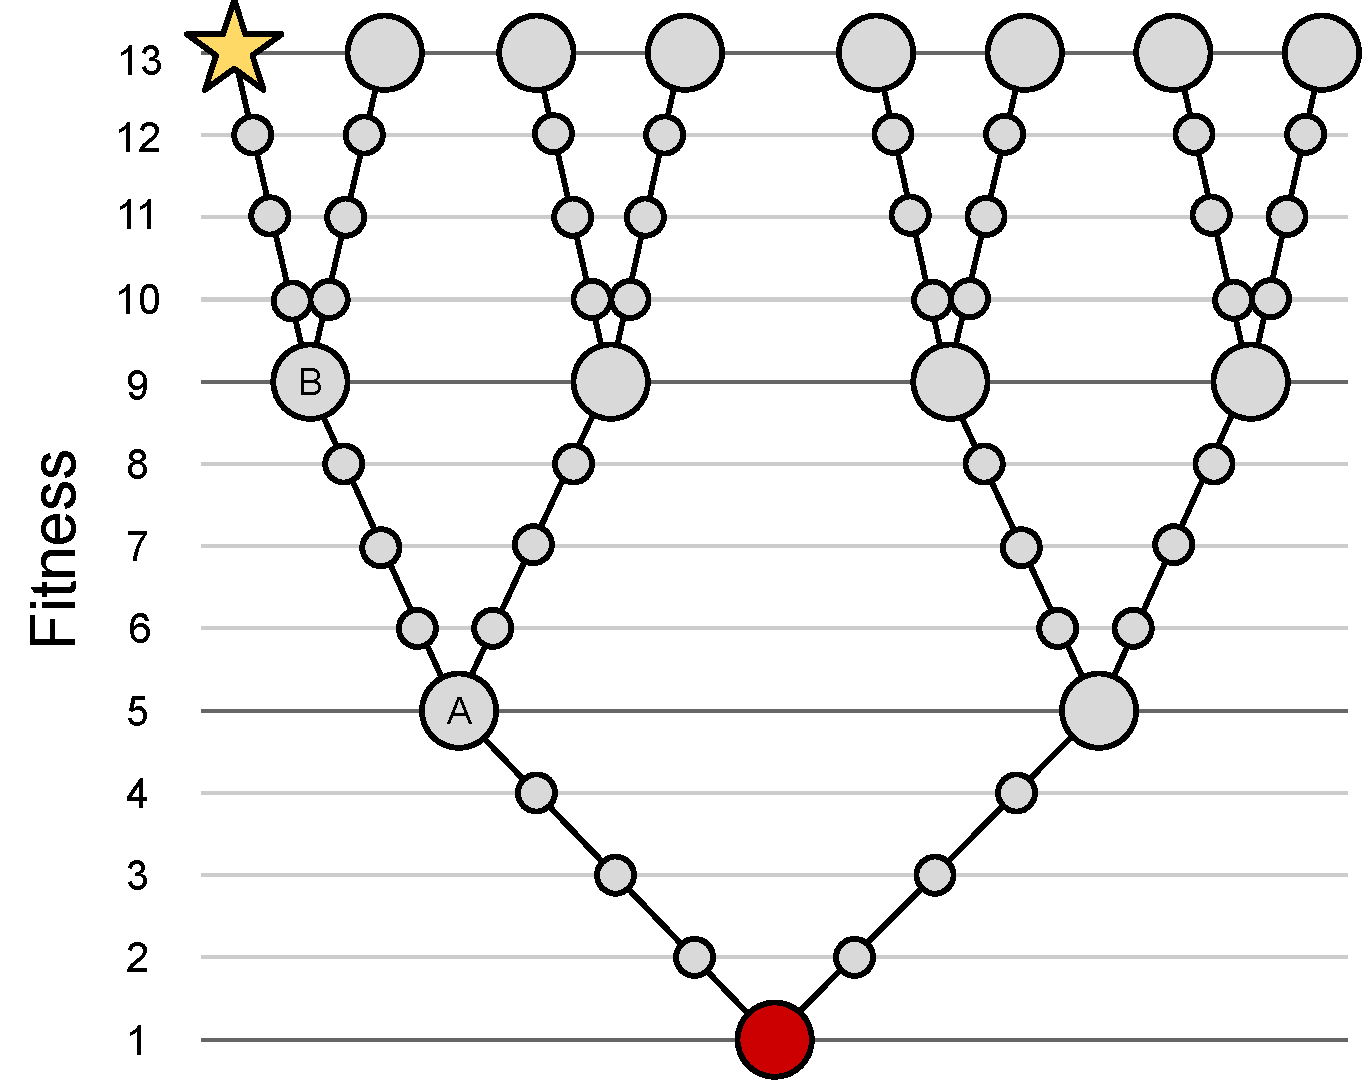
\includegraphics[width=0.65\textwidth]{06_conclusion/media/bst.pdf}
\end{center}
\caption{ 
A hypothetical fitness landscape in the form of a binary tree. 
Each node represents a particular genotype, and edges represent available mutations. 
Branch points, which have two higher-fitness neighbors, are shown larger than other nodes. 
The root node is shown in red, and two nodes are marked (A and B) for the in-text example. 
We can consider potentiation relative to the star, which can be reached with a series of mutations that use the left option at each branch point. 
}\label{fig:conclusion_binary_tree}
\end{figure}

To begin contemplating the ramifications of using absolute vs relative potentiation change, we can consider the simple fitness landscape in Figure \ref{fig:conclusion_binary_tree}.
If we assume a scenario with a low mutation rate and strong selection pressure, since fitness increases from the root node to the leaves, evolutionary theory dictates that all populations should evolve to a leaf node. 
%Fitness increases as we move from the root node to the leaves, so we expect all populations to evolve to a leaf node, assuming selection is strong enough. 
%Additionally, the population will reach two branching points over the course of evolution. 
Depending on the starting node, the population can encounter branching nodes over the course of evolution. 
Since each branching node has two neighboring nodes with higher yet equal fitness, we expect the population to go down each branch with 50\% probability. 
Here we consider the potentiation of the population evolving to reach the star node. 
In this example, potentiation for the star node from nodes between node B and the star are all approximately 100\%. 
Potentiation at the node B is expected to be 50\%, as the population will either evolve down the left or right branch. 
Similarly, potentiation is expected to be 25\% at node A and 12.5\% at the root node.
Thus, in terms of absolute potentiation differences along a trajectory from the root to the target node, potentiation will increase most moving from node B to the left at a 50\% increase. 
However, if we instead look at relative increases, moving off of the root, node A, and node B are all the same, doubling potentiation. 
This difference is demonstrated in Figure \ref{fig:conclusion_diff_types}

\begin{figure}[h!]
\begin{center}
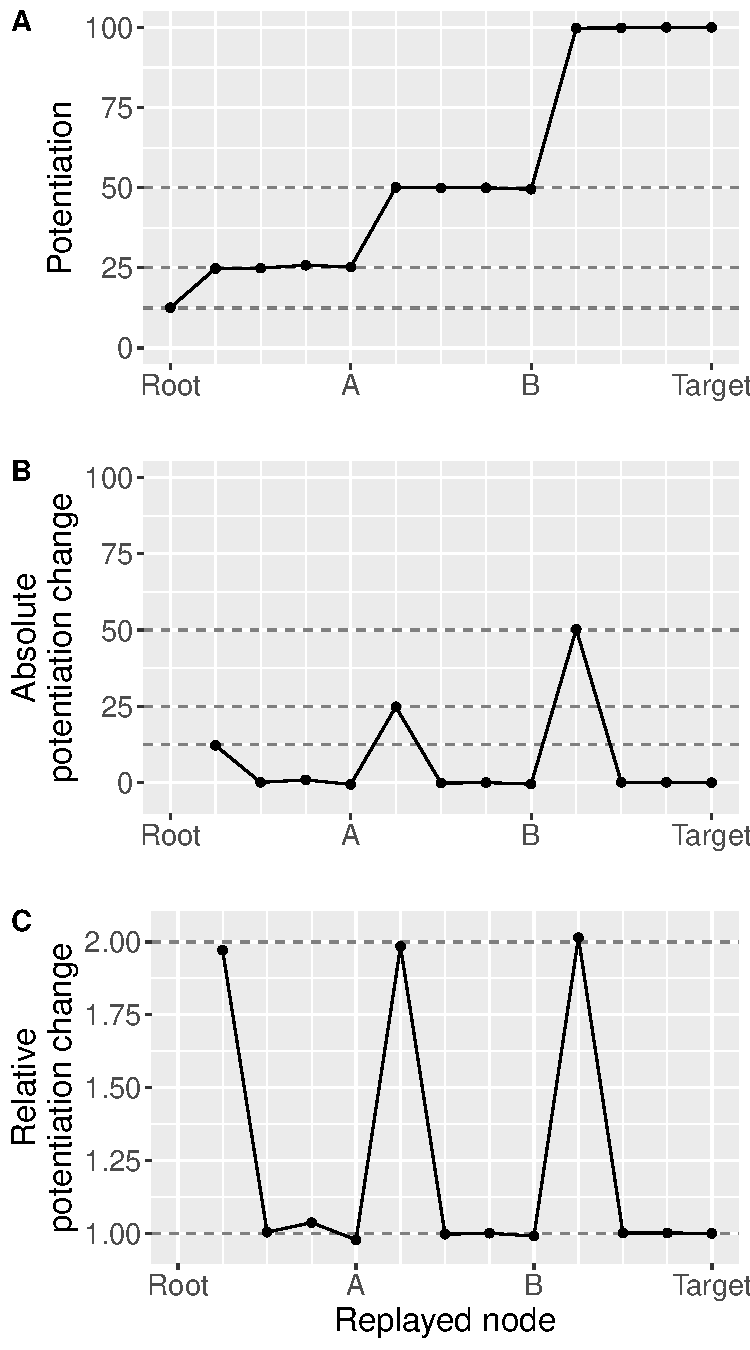
\includegraphics[width=0.58\textwidth]{06_conclusion/media/combined_plot_10k.pdf}
\end{center}
\caption{ 
Empirically measured potentiation of nodes from the fitness landscape in Figure \ref{fig:conclusion_binary_tree}. 
Subplot A shows potentiation for each node on the left side of the tree. 
Potentiation for a node is calculated as the percentage of replicates (out of 10,000) started with a full population of 100 organisms on that node that evolve to the target node after 500 generations of roulette selection.
Subplot B shows the absolute potentiation change when moving to each node, calculated as the difference between potentiation measured from the current position and the previous position. 
Subplot C shows the relative potentiation change, calculated as the potentiation measured at the current position divided by potentiation measured at the previous position.
}\label{fig:conclusion_diff_types}
\end{figure}

Considering these differences as absolute or relative are both valid approaches, in the same way that other measures such as epistasis can be measured either additively or multiplicatively. 
%In many cases we will be limited by the practical limitations of collecting enough data in order to measure potentiation with sufficient precision.
In Chapters \ref{chap:learning_case_studies} and \ref{chap:learning_distributions} I took an absolute approach as I wanted to analyze the overall potentiation of associative learning and how it changed. 
While the ``decision points'' encountered by evolution are interesting, they were not my main focus. 
What did prove relevant, however,is that because those experiments were conducted in Avida, I was limited to the resolution of my data.
I strained the computation resources available in order to do 50 replays for each potentiation measurement, meaning that I had a base resolution of $2\%$ intervals, before even considering noise.
A 5\% to 10\% increase can be significant and impactful, but the number of replicates needed to determine that difference with a high degree of statistical confidence were computationally infeasible. 
Future work should consider both approaches however, as large relative increases in potentiation might happen much earlier in the population's history and might provide additional insight. 

\subsection{Understanding factors that influence potentiation}

In Chapter \ref{chap:learning_case_studies}, I detailed the inner mechanics of the digital organisms and how the potentiating mutations paved the way for the evolution of learning. 
However, which dynamics factor into potentiation are still poorly understood. 
For example, my initial hypothesis was that most potentiating mutations would be deleterious or neutral, as beneficial mutations are likely to get selected and thus unlikely to influence the overall probability that the focal trait evolves. 
Chapter \ref{chap:learning_distributions} provided strong counter evidence, with 49 of 50 potentiating mutations being either beneficial or having no significant fitness effect. 
This raises the question: what other factors are at play in potentiation?

Three factors I want to draw attention to are the size of the mutational neighborhood, the mutation rate, and the size of the population.
Combined with the topography of the fitness landscape, these factors dictate the likelihood that a given mutation will appear. 
Specifically, as the number of neighbors increases, the mutation rate decreases, or the population size decreases, it becomes less likely that any given mutation will ever occur. 
As such, even the mutation with the highest possible fitness can be potentiating, as there is a chance \textit{it never appears} and thus selection cannot act upon it.
Additionally, even if a highly beneficial mutation appears, there is always the chance that it is lost to genetic drift.
Future studies should examine how varying each of these parameters in isolation changes the potentiation dynamics. 
In designing the experiment in Chapter \ref{chap:learning_case_studies}, I chose to use Avida partially because I was unsure how much complexity was needed to observe interesting potentiation changes. 
Chapter \ref{chap:adaptive_momentum} has demonstrated that this complexity is not required. 
While future work should observe potentiation in other complex systems, potentiation should also be studied in the simplest possible systems to conduct controlled studies like the ones mentioned here. 


\subsection{Improving evolutionary computation}

This dissertation is focused on improving our understanding of evolution as a process and the refinement of techniques to be applied back to wet lab studies. 
However, these techniques and ideas can also be applied to the problem-solving field of evolutionary computation (EC).
In order to improve efficiency and problem-solving ability, EC practitioners are constantly refining their evolving systems. 
Even beyond the initial design phase, most systems have a collection of parameters and operators to fine-tune the system for the particular task at hand. 
Optimizing the design decisions and parameter values of these systems is a continuous effort in EC research. 

How might a better understanding of historical contingency and potentiation improve our understanding in these systems? 
Let us imagine that we want to test the effects of adding new mutational operators to our EC system. 
A proper first step would be to run a two treatment experiment: one batch of experiments that have access to these new operators and a control treatment that does not. 
With enough replicates, we should see if our changes improve the problem solving success of our system. 
Indeed, we could dive further and test these new operators in isolation or in combination, to disentangle which operators improve our success. 

To consider the benefit of adopting a history-based mindset, we must switch from asking \textit{if} these new mutational operators improve our problem solving success to asking \textit{how} the new operators improve our evolutionary search.
We can, and often do, make inferences about what events might have been critical to a replicate's success. 
For example, we might identify a gene duplication event occurring shortly before the focal trait evolves.
However, only by experimentally testing the effect of accumulated history can we verify which specific events were pivotal in the population's ultimate success and which were mere coincidence. 
In our example, the gene duplication mentioned above might have helped, but it also may have followed another mutation whose importance is harder to detect. 
It is this interplay of dynamics that we aim to clarify. 
By leveraging these techniques, we may be able to nail down interactions between constituent parts, such as our mutation operators, that are beneficial and that we want to encourage via our design choices and parameters settings. 

However, with this increased analytic power comes an increase in computational requirements. 
Techniques such as replay experiments have the potential to deliver critical insights into EC systems, but they are too computationally expensive to conduct regularly. 
As such, future work should aim to identify cases where these techniques are most useful, so practitioners can leverage them when they are the correct tool for the job. 

%\subsection{Quantifying tradeoffs}

\subsection{Quantifying evolvability}

Generally, analytic replay experiments have focused on the potentiation of beneficial traits. 
This leads to a simple observation: if the focal trait is beneficial, an increase in its potentiation is likely to correspond to an increase in the long-term fitness of the lineage, depending on the alternative trajectories that could have been taken.
Though we lack an agreed upon definition of evolvability \citep{pigliucciEvolvabilityEvolvable2008}, here I use the definition of \citet{payneCausesEvolvabilityTheir2019}: ``the ability of a biological system to produce phenotypic variation that is both heritable and adaptive''.
Thus, I argue that an increase in average long-term fitness constitutes an increase in evolvability.

I am not the first to combine the ideas of evolvability and historical contingency. 
\citet{woodsSecondorderSelectionEvolvability2011} were among the first to leverage analytic replay experiments, and they used these replays to test the long-term evolvability of two clades of \textit{E. coli}.
In the original replicate, the clade that eventually won had lower fitness at the time of sampling. 
Replay experiments started from that original point demonstrated that the ``eventual winner'' clade consistently evolved higher fitness despite its lower initial fitness -- it was more \textit{evolvable}.

\begin{figure}[h!]
\begin{center}
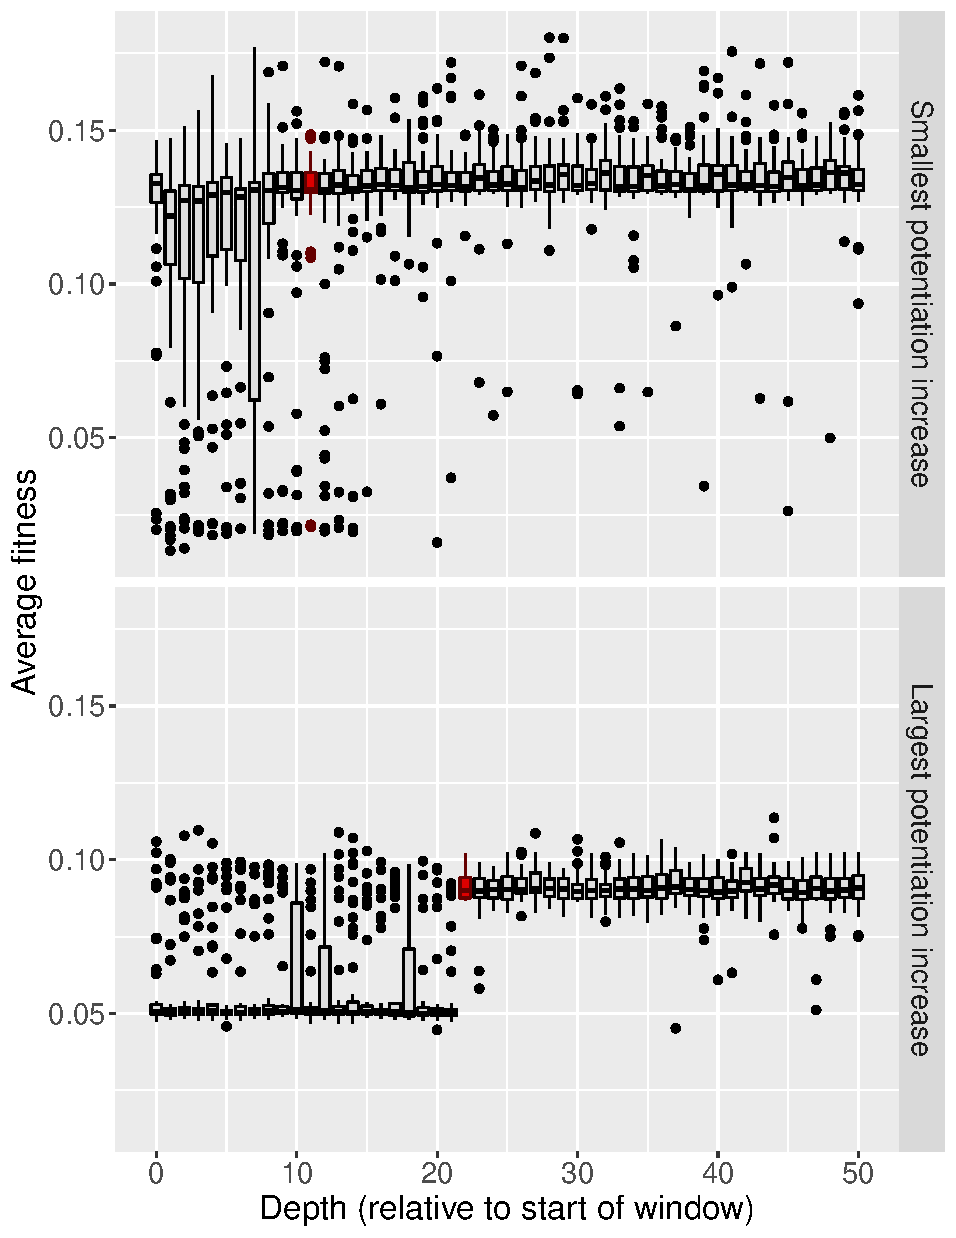
\includegraphics[width=0.75\textwidth]{06_conclusion/media/evolvability.pdf}
\end{center}
\caption{ 
Two examples of evolvability data from the targeted replays of Chapter \ref{chap:learning_distributions}. 
A boxplot is shown for each depth replayed in the targeted replays, corresponding to the average fitness at the end of each of the 50 replicates replayed from that depth. 
The red boxplot shows the potentiating step. 
Two lineages are shown, one with a small potentiation increase (20 percentage points) and little change in long-term fitness, and another with a large potentiation increase (88 percentage points) and a stark increase in long-term fitness with the potentiating step. 
}\label{fig:conclusion_evolvability}
\end{figure}


In conducting multiple replay experiments, I have realized that these systems are ripe for further studies in evolvability. 
We must first consider the concept of ``evolvability-enhancing muations'' as introduced by \citep{wagnerEvolvabilityenhancingMutationsFitness2023}. 
Evolvability-enhancing mutations are defined as mutations whose one-step mutational neighborhood has a higher average fitness than the one-step neighborhood of the wild type.
As noted by the author, we could also define these evolvability-enhancing mutations using a two-step, three-step, or larger mutational neighborhood. 
Increasing the range of the mutational neighborhood would overcome issues such as evolvability-enhancing mutations that lead to local fitness peaks, limiting long-term fitness.

Unfortunately, performing a N-step mutant analysis becomes intractable on most fitness landscapes for, at most, $N > 2$.
Thankfully, we can make a simplification: what if we only consider the mutational trajectories that are most likely? 
This is exactly what replay experiments do; each replay replicate samples the fitness landscape that is reachable from the starting condition in a given amount of time.
While we are only sampling a fraction of the possible trajectories, the sample should be representative of what will evolve from the starting condition. 


Finally, conducting these studies requires \textit{little to no additional work}.
If a replay experiment is conducted to observe the potentiation dynamics of a lineage for a particular trait, the only additional step is to also evaluate fitness at the end of each replay replicate. 
In Chapter \ref{chap:learning_distributions}, I had to quantify fitness in order to determine if the replay replicates evolved learning. 
As such, \textit{these data already contain information on evolvability}.
Unfortunately, a full analysis of these data are out of scope for this dissertation. 
A preliminary examination is shown in Figure \ref{fig:conclusion_evolvability}, exhibiting the long-term fitness of the replays from two lineages. 
One lineage, which had only a 20 percentage point increase in potentiation, sees little change in the long-term fitness at the potentiating step. 
The second lineage, which had the largest single-step potentiation increase (88 percentage points), sees a substantial increase in long-term fitness. 
When we consider these results through the lens of potentiation, we see that the higher-fitness trajectories were always present, potentiating mutations are simply biasing evolution toward these high-fitness areas, and thus, increasing evolvability. 
Future work should further explore these dynamics; my hypothesis is that the increase in potentiation and the increase in long-term fitness should be correlated in systems where the potentiation trait being measured represents a highly beneficial adaptation. 

% Example for splitting the thesis into a few parts (I don't use this -- AJF)
% \part{Designing Computational Infrastructure to Enable Scalable Digital Multicellularity Experiments} \label{part:infrastructure}

%%%%%%%%%%%%%%%%%%%%%%%%%%%%%%%%%%%%%%%%%%%%%%%%%%%%%%%%%
% == Bibliography ==
% Make sure we're linking to the correct page... https://tex.stackexchange.com/questions/74439/table-of-contents-incorrect-page-numbering
\clearpage
\phantomsection
\begin{singlespace}
\addcontentsline{toc}{chapter}{BIBLIOGRAPHY}
\renewcommand{\bibsection}{\centerline{\textbf{BIBLIOGRAPHY}}}
\bibliographystyle{apalike}% your bst file here
\bibliography{ferguson_dissertation, supplements} %your bib file here
\end{singlespace}

%%%%%%%%%%%%%%%%%%%%%%%%%%%%%%%%%%%%%%%%%%%%%%%%%%%%%%%%%
% == Appendices, if necessary ==
% Make sure we're linking to the correct page... https://tex.stackexchange.com/questions/74439/table-of-contents-incorrect-page-numbering
\clearpage
\phantomsection
\appendix
\renewcommand\chaptername{APPENDIX} % I was asked to make this all caps - AJF
% ensure appendix chapters are labeled appendix instead of chapter in toc
% adapted from https://tex.stackexchange.com/a/56845
% see also https://tex.stackexchange.com/a/50037

\begin{filecontents}{toc-chapter-to-appendix.tex}
%\addtocontents{toc}{\protect\renewcommand{\protect\cftchappresnum}{\appendixname\space}}
% https://latex.org/forum/viewtopic.php?t=11871, remove appendix title - AJF
\addcontentsline{toc}{chapter}{APPENDIX}
%\addtocontents{toc}{\protect\setcounter{tocdepth}{-1}}
\end{filecontents}
\include{toc-chapter-to-appendix.tex}

% Remove Appendix letters (e.g., Appendix A -> Appendix)
% This was requested as I only have one appendix "chapter" - AJF
% https://tex.stackexchange.com/a/21320
\renewcommand\thechapter{}
\renewcommand\thesection{\arabic{section}}
%%% Use format: \include{<file here>(No Extension)}
\begingroup
\let\clearpage\relax
\centerline{\textbf{APPENDIX}}
\vspace{0.5em}
%\chapter*{\textbf{APPENDIX}\linebreak Plots of potentiation over time}
\chapter*{Plots of potentiation over time}
\label{chap:app_a}
\endgroup

\begin{figure}[!h]
    \begin{center}
    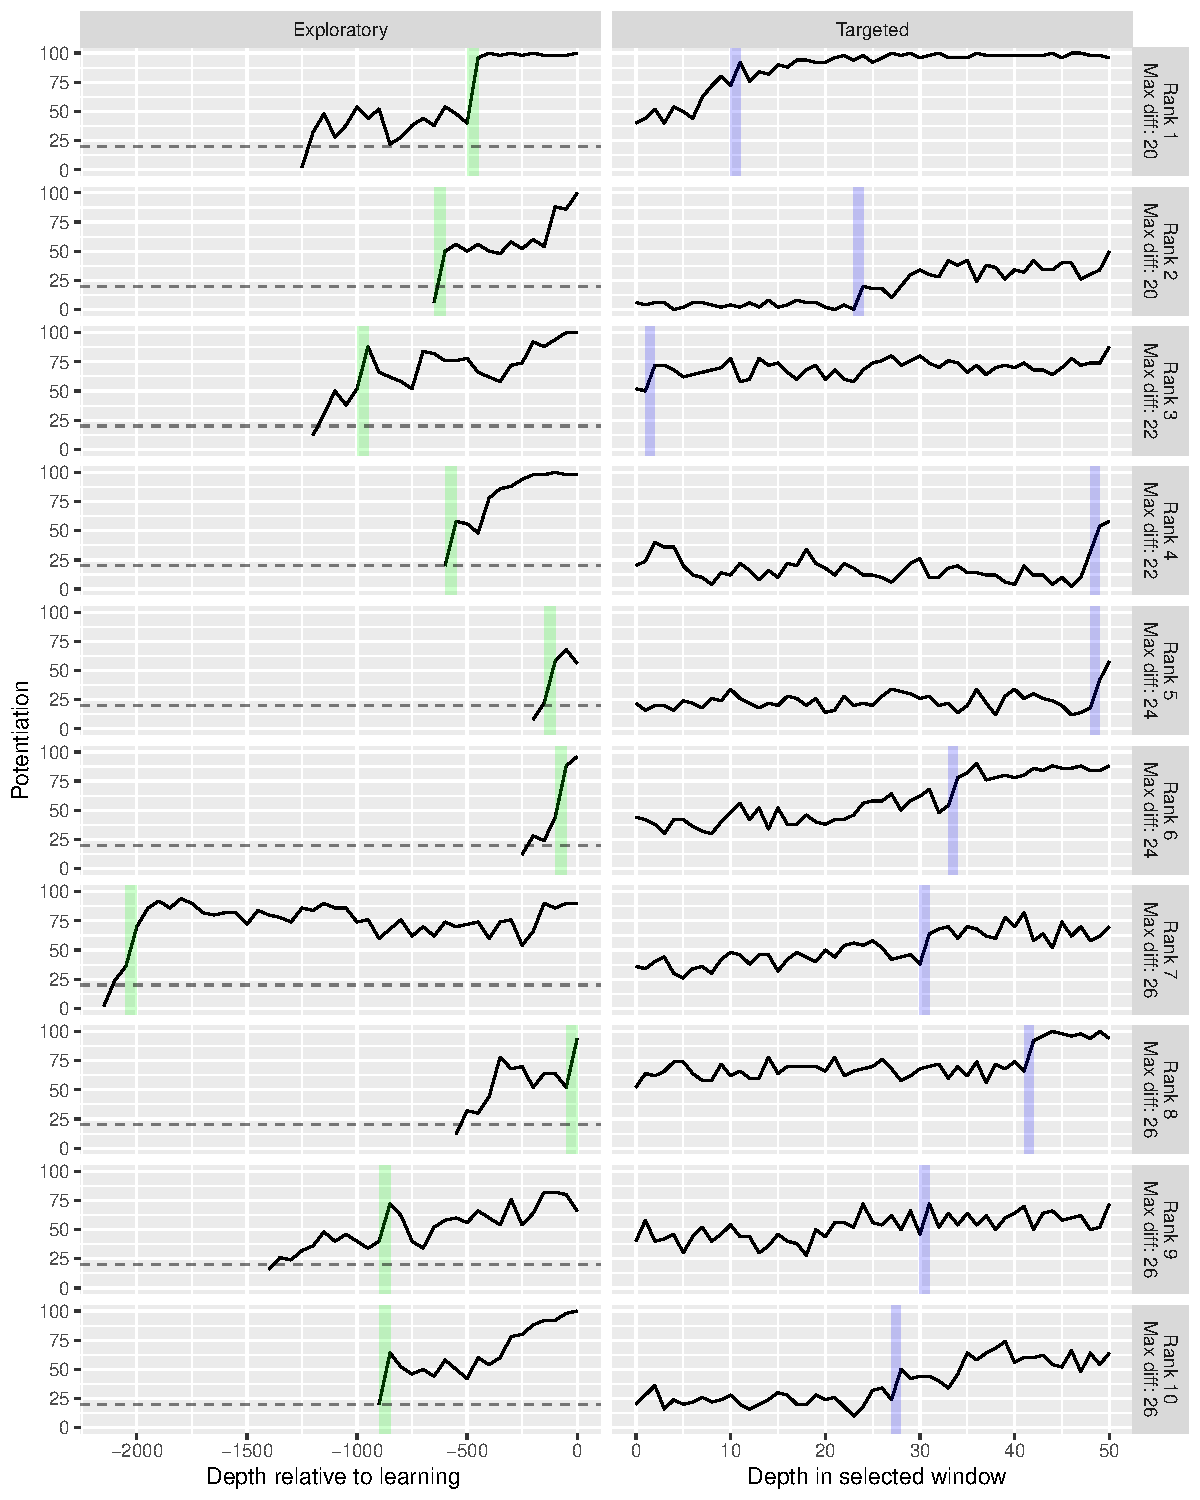
\includegraphics[width=0.85\textwidth]{07_appendix_potentiation_over_time/media/reps_1_10.pdf}
    \caption{Potentiation over time plots from Chapter \ref{chap:learning_distributions}.
    Left panes show exploratory replays, with a green rectangle indicating the 50-step window with the largest increase in potentiation. 
    Right panes show targeted replays, with the blue rectangle highlighting the largest single-step potentiation increase.
    Plots are ordered by the maximum single-step potentiation difference. }
    \label{fig:app_a_1_10}
    \end{center}
\end{figure}

\begin{figure}[!h]
    \begin{center}
    \includegraphics[width=0.9\textwidth]{07_appendix_potentiation_over_time/media/reps_11_20.pdf}
    \caption{Potentiation over time plots from Chapter \ref{chap:learning_distributions}.
    Left panes show exploratory replays, with a green rectangle indicating the 50-step window with the largest increase in potentiation. 
    Right panes show targeted replays, with the blue rectangle highlighting the largest single-step potentiation increase.
    Plots are ordered by the maximum single-step potentiation difference.}
    \label{fig:app_a_11_20}
    \end{center}
\end{figure}

\begin{figure}[!h]
    \begin{center}
    \includegraphics[width=0.9\textwidth]{07_appendix_potentiation_over_time/media/reps_21_30.pdf}
    \caption{Potentiation over time plots from Chapter \ref{chap:learning_distributions}.
    Left panes show exploratory replays, with a green rectangle indicating the 50-step window with the largest increase in potentiation. 
    Right panes show targeted replays, with the blue rectangle highlighting the largest single-step potentiation increase.
    Plots are ordered by the maximum single-step potentiation difference.}
    \label{fig:app_a_21_30}
    \end{center}
\end{figure}

\begin{figure}[!h]
    \begin{center}
    \includegraphics[width=0.9\textwidth]{07_appendix_potentiation_over_time/media/reps_31_40.pdf}
    \caption{Potentiation over time plots from Chapter \ref{chap:learning_distributions}.
    Left panes show exploratory replays, with a green rectangle indicating the 50-step window with the largest increase in potentiation. 
    Right panes show targeted replays, with the blue rectangle highlighting the largest single-step potentiation increase.
    Plots are ordered by the maximum single-step potentiation difference.}
    \label{fig:app_a_31_40}
    \end{center}
\end{figure}

\begin{figure}[!h]
    \begin{center}
    \includegraphics[width=0.9\textwidth]{07_appendix_potentiation_over_time/media/reps_41_50.pdf}
    \caption{Potentiation over time plots from Chapter \ref{chap:learning_distributions}.
    Left panes show exploratory replays, with a green rectangle indicating the 50-step window with the largest increase in potentiation. 
    Right panes show targeted replays, with the blue rectangle highlighting the largest single-step potentiation increase.
    Plots are ordered by the maximum single-step potentiation difference.}
    \label{fig:app_a_41_50}
    \end{center}
\end{figure}

\begin{figure}[!h]
    \begin{center}
    \includegraphics[width=0.9\textwidth]{07_appendix_potentiation_over_time/media/non_learning.pdf}
    \caption{Potentiation over time plots from Chapter \ref{chap:learning_distributions} for replayed replicates that did not originally evolve learning.
    Lines show the potentiation of each possible behavior. 
    One replicate is shown per row, and rows are ordered by final evolved behavior.
    Acronyms: BH: bet-hedged / bet hedging; EC: error correction. 
    Note that seed 3,440 evolved bet-hedged error correction, even though it was a very low probability at the latest replay point (0 of 50 replay replicates). 
    }
    \label{fig:app_a_non_learning}
    \end{center}
\end{figure}

\end{doublespace}
\end{document}
